\documentclass[11pt]{book}
\oddsidemargin 0in
\evensidemargin 0in
\marginparwidth 0in
\textheight 8in
\textwidth 6.5in
\topmargin 0in
\headheight 14pt
\usepackage{amssymb,amsmath,amsthm,fancyhdr,supertabular,longtable,hhline,mathtools}
\usepackage{colortbl}
\usepackage{import, multicol,boxedminipage}
\usepackage{chapterfolder}
\usepackage[metapost,truebbox]{mfpic}
\usepackage[pdflatex]{graphicx}
\usepackage{makeidx}
\usepackage[colorlinks, hyperindex, plainpages=false, linkcolor=blue, urlcolor=blue, pdfpagelabels]{hyperref}
\usepackage[all]{hypcap}
\usepackage{cancel}
\usepackage{sectsty}
\usepackage{textcomp}
\allsectionsfont{\mdseries \scshape}
\definecolor{ResultColor}{gray}{0.9}
\theoremstyle{definition}  % this prevents the text in definitions, theorems, and corollaries from being italicized
\newtheorem{defn}{\sc Definition}[chapter]
\newtheorem{thm}{\sc Theorem}[chapter]
\newtheorem{cor}[thm]{\sc Corollary}
\newtheorem{eqn}{\sc Equation}[chapter]
\newtheorem{ex}{\sc Example}[section]
\newtheorem{fig}{\sc Figure}[chapter]
\setlength{\parindent}{0in}
\newcommand{\bbm}{\begin{boxedminipage}{6.41in}}
\newcommand{\ebm}{\end{boxedminipage}}
\usepackage{array}
\setlength{\extrarowheight}{2pt}
\allowdisplaybreaks[2]
\allsectionsfont{\mdseries \scshape}
%Below is for Helvetica (scaled): 
\usepackage[scaled=.92]{helvet}   
\renewcommand{\familydefault}{\sfdefault}  %makes the text of the book sans serif
\usepackage[helvet]{sfmath}  %makes the math in the book sans serif
\allsectionsfont{\sffamily}  %makes the chapter and section titles sans serif

\makeatletter
\newcases{mycases}{\quad}{%
  \hfil$\m@th\displaystyle{##}$}{$\m@th\displaystyle{##}$\hfil}{\lbrace}{.}
\makeatother

\begin{document}
\newcounter{HW}
\newcounter{HWindent}
\renewcommand{\textinterrobang}{$! \! \! ?$}


\chapter{\sc Rational Functions}

\section{Rational Expressions and Equations}

\import{./AlgebraAppendix/}{AppRatExpEqus}


\section{Introduction to Rational Functions}

\mfpicnumber{1}
\opengraphsfile{IntroRational}

\setcounter{footnote}{0}

\label{IntroRational}


If we add, subtract, or multiply polynomial functions, the result is another polynomial function.  When we divide polynomial functions, however, we may not get a polynomial function.   The result of dividing two polynomials is a   \index{rational function} \textbf{rational function}, so named because rational functions  are \textit{ratios} of polynomials.

\smallskip

\colorbox{ResultColor}{\bbm

\begin{defn}  \label{rationalfunction} A \textbf{rational function} is a function which is the ratio of polynomial functions.  Said differently, $r$ is a rational function if it is of the form \index{function ! rational}

\[ r(x) = \dfrac{p(x)}{q(x)},\]

where $p$ and $q$ are polynomial functions.\footnote{According to this definition, all polynomial functions are also  rational functions. (Take $q(x) = 1$).}

\end{defn}

\ebm}

\subsection{Laurent Monomial Functions}
\label{LaurentMonomialFunctionsSection}

As with polynomial functions, we begin our study of rational functions with what are, in some sense, the building blocks of rational functions, \index{monomial function ! Laurent}\index{function ! monomial ! Laurent}\textbf{Laurent monomial functions}.  

\colorbox{ResultColor}{\bbm

\begin{defn}  \label{laurentmonomialfunction} A \textbf{Laurent monomial function} is either a monomial function (see Definition \ref{monomialfunction}) or a function of the form $f(x) = \dfrac{a}{x^n} = ax^{-n}$ for $n \in \mathbb{N}$.

\end{defn}

\ebm}

Laurent monomial functions are named in honor of \href{https://en.wikipedia.org/wiki/Pierre_Alphonse_Laurent}{\underline{Pierre Alphonse Laurent}} and generalize the notion of `monomial function' from Chapter \ref{PolynomialFunctions} to terms with negative exponents. Our study of these functions begins with an analysis of   $r(x) = \frac{1}{x} = x^{-1}$, the reciprocal function. The first item worth  noting is that $r(0)$ is not defined owing to the presence of $x$  in the denominator.  That is, the domain of $r$ is $\{ x \in \mathbb{R} \, | \, x \neq 0\}$ or, using interval notation, $(-\infty, 0) \cup (0, \infty)$.   Of course excluding $0$ from the domain of $r$ serves only to pique our curiosity about the behavior of $r(x)$ when $x \approx 0$.  Thinking from a number sense perspective, the closer the denominator of $\frac{1}{x}$ is to $0$, the larger the value of the  fraction (in absolute value.)\footnote{Technically speaking, $-1 \times 10^{117}$ is a `small' number (since it is very far to the left on the number line.)  However, it's absolute value, $1 \times 10^{117}$ is very large.}  So it stands to reason that as $x$ gets closer and closer to $0$, the values for $r(x) = \frac{1}{x}$ should grow larger and larger (in absolute value.)  This is borne out in the table below on the left where it is apparent that for $x \approx 0$, $r(x)$ is becoming unbounded.  

As we investigate the end behavior of $r$, we find that as $x \rightarrow \pm \infty$, $r(x) \approx 0$. Again, number sense agrees here with the data, since as the denominator of $\frac{1}{x}$ becomes unbounded, the value of the fraction should diminish.  That being said, we could ask if the graph ever reaches the $x$-axis.  If we attempt to solve $y = r(x) = \frac{1}{x} = 0$. we arrive at the contradiction $1 = 0$ hence, $0$ is not in the range of $r$.  Every other real number besides $0$ is in the range of $r$, however.  To see this, let $c \neq 0$ be a real number.  Then $\frac{1}{c}$ is defined and, moreover, $r \left(\frac{1}{c} \right) = \frac{1}{(1/c)} = c$.  This shows $c$ is in the range of $r$.  Hence, the range of $r$ is $\{ y \in \mathbb{R} \, | \, y \neq 0\}$ or, using interval notation,  $(-\infty, 0) \cup (0, \infty)$.  

\begin{center}
\begin{tabular}{m{2in}m{2in}m{2in}}

$\begin{array}{|r||c|}  \hline

  x & r(x) = \frac{1}{x}  \\ \hline
 -0.01& -100  \\  \hline
 -0.001 & -1000  \\  \hline 
 -0.0001 & -10000  \\  \hline 
 -0.00001 & -100000 \\  \hline 
0 & \text{undefined} \\  \hline
0.00001 & 100000 \\  \hline  
0.0001 & 10000  \\  \hline 
 0.001 & 1000  \\  \hline 
 0.01 & 100  \\  \hline
  \end{array} $
  
  &
  
  $\begin{array}{|r||c|}  \hline

  x & r(x) = \frac{1}{x}  \\ \hline
 -100000 & -0.00001  \\  \hline 
 -10000 &  -0.0001 \\  \hline 
 -1000 & -0.001  \\  \hline 
 -100 & -0.01  \\  \hline
0 & \text{undefined} \\  \hline
 100 & 0.01  \\  \hline
 1000 & 0.001  \\  \hline 
 10000 & 0.0001 \\  \hline
 100000 & 0.00001  \\  \hline  
  \end{array} $
  
  &
  
\begin{mfpic}[15]{-5}{5}{-5}{5}
\axes
\scriptsize
\tlabel[cc](5, -0.5){$x$}
\tlabel[cc](0.5, 5){$y$}
\tlabel[cc](-2, -1.5){$(-1,-1)$}
\tlabel[cc](2, 1.5){$(1,1)$}
\normalsize
\penwd{1.25pt}
\arrow \reverse \arrow \function{-5,-0.2,0.1}{1/x}
\arrow \reverse \arrow \function{0.2,5,0.1}{1/x}
\point[4pt]{(-1,-1), (1,1)}
\tcaption{\scriptsize $y=r(x) = \frac{1}{x}$}
\end{mfpic}\\



\end{tabular}

\end{center}

In order to more precisely describe the behavior near $0$, we say `as $x$ approaches $0$ \textit{from the left},' written as $x \rightarrow 0^{-}$, the function values $r(x) \rightarrow -\infty$. By `from the left' we mean we are considering $x$-values slightly to the \textit{left} of $0$ on the number line, such as   $x = -0.001$ and $x = -0.0001$ in the table above. If we think of these numbers as all being $x$-values where  $x  = \text{`$0-$ a little bit'}$, the  the `$-$' in the notation `$x \rightarrow 0^{-}$' makes better sense.  The notation to describe the $r(x)$ values, $r(x) \rightarrow -\infty$, is used here in the same manner as it was in Section \ref{GraphsofPolynomials}.  That is, as  $x \rightarrow 0^{-}$,   the values $r(x)$ are becoming unbounded in the negative direction.  

Similarly, we say `as $x$ approaches $0$ \textit{from the right},' that is as $x \rightarrow 0^{+}$, $r(x) \rightarrow \infty$.  Here `from the right' means we are using $x$ values slightly to the \textit{right} of $0$ on the number line:  numbers such as $x =0.001$ which could be described as `$0 + \text{a little bit}$.'   For these values of $x$, the values of $r(x)$ become unbounded (in the positive direction) so we write $r(x)  \rightarrow \infty$ here. 

We can also use this notation to describe the end behavior, but here the numerical roles are reversed.  We see as $x \rightarrow -\infty$, $r(x) \rightarrow 0^{-}$ and as $x \rightarrow \infty$, $r(x) \rightarrow 0^{+}$.

The way we describe what is happening graphically is to say the line $x = 0$ is a  \index{asymptote ! vertical ! intuitive definition of}\index{vertical asymptote ! intuitive definition of}\textbf{vertical asymptote}  to the graph of $y = r(x)$ an the line $y = 0$ is a \index{asymptote ! horizontal ! intuitive definition of}\index{horizontal asymptote ! intuitive definition of}\textbf{horizontal asymptote} to the graph of $y = r(x)$.  Roughly speaking, asymptotes are lines which approximate functions as either the inputs our outputs become unbounded.  While defined more precisely using the language of Calculus, we do our best to formally define vertical and horizontal asymptotes below.

\colorbox{ResultColor}{\bbm

\begin{defn} \label{va} The line $x=c$ is called a \index{asymptote ! vertical ! formal definition of}\index{vertical asymptote ! formal definition of}\textbf{vertical asymptote} of the graph of a function $y=f(x)$ if as $x \rightarrow c^{-}$ or as $x \rightarrow c^{+}$, either $f(x) \rightarrow \infty$ or $f(x) \rightarrow -\infty$.

\end{defn}
\ebm}

\medskip

\colorbox{ResultColor}{\bbm

\begin{defn} \label{ha} The line $y=c$ is called a \index{asymptote ! horizontal ! formal definition of}\index{horizontal asymptote ! formal definition of}\textbf{horizontal asymptote} of the graph of a function $y=f(x)$ if as $x \rightarrow -\infty$ or as $x \rightarrow \infty$, $f(x) \rightarrow c$.


\end{defn}
\ebm}

\medskip

Note that in Definition \ref{ha}, we write $f(x) \rightarrow c$ (not $f(x) \rightarrow c^{+}$ or $f(x) \rightarrow c^{-}$) because we are unconcerned from which direction the values $f(x)$ approach the value $c$, just as long as they do so.  As we shall see, the graphs of rational functions may, in fact, \textit{cross} their horizontal asymptotes.  If this happens, however,  it does so only a \textit{finite} number of times (at least in this chapter), and so for each choice of $x \rightarrow -\infty$ and $x \rightarrow \infty$, $f(x)$ will approach $c$ from either below (in the case $f(x) \rightarrow c^{-}$) or above (in the case $f(x) \rightarrow c^{+}$.)  We leave $f(x) \rightarrow c$ generic in our definition, however, to allow this concept to apply to less tame specimens in the Precalculus zoo, one that cross horizontal asymptotes an infinite number of times.\co{\footnote{See Exercise \ref{exploregraphslast} in Section \ref{GraphsofSineandCosine}.}}


The behaviors illustrated in the graph $r(x) = \frac{1}{x}$ are typical of functions of the form $f(x) = \frac{1}{x^n} = x^{-n}$ for natural numbers, $n$.  As with the monomial functions discussed in Section \ref{GraphsofPolynomials}, the patterns that develop primarily depend on whether $n$ is odd or even.  Having thoroughly discussed the graph of $y = \frac{1}{x} = x^{-1}$, we graph it along with $y = \frac{1}{x^3} = x^{-3}$ and $y = \frac{1}{x^5} = x^{-5}$ below.  Note the points $(-1,-1)$ and $(1,1)$ are common to all three graphs as are the asymptotes $x = 0$ and $y = 0$.  As the $n$ increases, the graphs become steeper for $|x| < 1$  and flatten out more quickly for $|x|>1$.  Both the domain and range in each case appears to be $(-\infty, 0) \cup (0, \infty)$.  Indeed, owing to the $x$ in the denominator of $f(x) = \frac{1}{x^n}$, $f(0)$, and only $f(0)$,  is undefined. Hence the domain is $(-\infty, 0) \cup (0, \infty)$.  When thinking about the range, note the equation  $f(x)= \frac{1}{x^n}  = c$ has the solution $x = \sqrt[n]{\frac{1}{c}}$ as long as $c \neq 0$.  Thus means $f\left( \sqrt[n]{\frac{1}{c}} \right) = c$ for every nonzero real number $c$.  If $c = 0$, we are in the same situation as before:  $\frac{1}{x^n} = 0$ has no real solution.  This establishes the range is $(-\infty, 0) \cup (0, \infty)$.  Finally, each of the graphs appear to be symmetric about the origin.  Indeed, since $n$ is odd, $f(-x) = (-x)^{-n} = (-1)^{-n} x^{-n} = -x^{-n} = -f(x)$, proving every member of this function family is odd.  

\begin{tabular}{m{2.75in}m{1.25in}m{1.25in}m{1.25in}}

$\begin{array}{|r||c|c|c|}  \hline

 x &  \frac{1}{x} = x^{-1} & \frac{1}{x^3} = x^{-3} & \frac{1}{x^5} = x^{-5} \\ \hline
 -10 & -0.1 &-0.001& -0.00001  \\  \hline
 -1 & -1 & -1&  -1\\  \hline
 -0.1 & -10 & -1000&  -100000 \\  \hline
 0 &  \text{undefined} &  \text{undefined}  &  \text{undefined}  \\  \hline
 0.1 & 10 & 1000&  100000 \\  \hline
 1 & 1 & 1&  1\\  \hline
 10 & 0.1 & 0.001& 0.00001  \\  \hline

\end{array}$

&

\begin{mfpic}[9]{-5}{5}{-5}{5}
\axes
\scriptsize
\tlabel[cc](5, -0.5){$x$}
\tlabel[cc](-0.5, 5){$y$}
\normalsize
\penwd{1.25pt}
\arrow \reverse \arrow \function{-5,-0.2,0.1}{1/x}
\arrow \reverse \arrow \function{0.2,5,0.1}{1/x}
\point[4pt]{(-1,-1), (1,1)}
\tcaption{\scriptsize $y=\frac{1}{x} = x^{-1}$}
\end{mfpic}

&

\begin{mfpic}[9]{-5}{5}{-5}{5}
\axes
\scriptsize
\tlabel[cc](5, -0.5){$x$}
\tlabel[cc](-0.5, 5){$y$}
\normalsize
\penwd{1.25pt}
\arrow \reverse \arrow \function{-5,-0.58,0.1}{1/(x**3)}
\arrow \reverse \arrow \function{0.58,5,0.1}{1/(x**3)}
\point[4pt]{(-1,-1),  (1,1)}
\tcaption{\scriptsize $y=\frac{1}{x^3} = x^{-3}$}
\end{mfpic}

&

\begin{mfpic}[9]{-5}{5}{-5}{5}
\axes
\scriptsize
\tlabel[cc](5, -0.5){$x$}
\tlabel[cc](-0.5, 5){$y$}
\normalsize
\penwd{1.25pt}
\arrow \reverse \arrow \function{-5,-0.72,0.1}{1/(x**5)}
\arrow \reverse \arrow \function{0.725,5,0.1}{1/(x**5)}
\point[4pt]{(-1,-1), (1,1)}
\tcaption{\scriptsize $y=\frac{1}{x^5} = x^{-5}$}
\end{mfpic} \\

\end{tabular}

We repeat the same experiment with functions of the form $f(x) = \frac{1}{x^{n}} = x^{-n}$ where $n$ is even. $y = \frac{1}{x^2} = x^2$, $y = \frac{1}{x^4} = x^{-4}$ and $y = \frac{1}{x^6} = x^{-6}$.  These graphs all share the points $(-1,1)$ and $(1,1)$, and asymptotes $x = 0$ and $y = 0$.  The same remarks about the steepness for $|x|<1$ and the flattening for $|x|>1$ also apply. For the same reasons as given above, the domain of each of these functions is $(-\infty, 0) \cup (0, \infty)$.  When it comes to the range, the fact $n$ is even tells us tere are  solutions to $\frac{1}{x^n} = c$ only if $c>0$. It follows that the range is $(0, \infty)$ for each of these functions.  Concerning symmetry, as $n$ is even, $f(-x) = (-x)^{-n} = (-1)^{-n} x^{-n} = x^{-n} = f(x)$, proving each member of this function family is even.  Hence, all of the graphs of these functions is symmetric about the $y$-axis.


\begin{tabular}{m{2.75in}m{1.25in}m{1.25in}m{1.25in}}

$\begin{array}{|r||c|c|c|}  \hline

 x &  \frac{1}{x^2} = x^{-2} & \frac{1}{x^4} = x^{-4} & \frac{1}{x^6} = x^{-6} \\ \hline
 -10 &0.01 &0.0001& 1 \times 10^{-6}  \\  \hline
 -1 & 1 & 1&  1\\  \hline
 -0.1 & 100 & 10000 &  1 \times 10^{6} \\  \hline
 0 &  \text{undefined} &  \text{undefined}  &  \text{undefined}  \\  \hline
0.1 & 100 & 10000 &  1 \times 10^{6} \\  \hline
 1&  1 & 1&  1 \\  \hline
10 &0.01 &0.0001& 1 \times 10^{-6}  \\  \hline

\end{array}$

&

\begin{mfpic}[9]{-5}{5}{-1}{9}
\axes
\scriptsize
\tlabel[cc](5, -0.5){$x$}
\tlabel[cc](0, 9.5){$y$}
\normalsize
\penwd{1.25pt}
\arrow \reverse \arrow \function{-5,-0.3333,0.1}{1/(x**2)}
\arrow \reverse \arrow \function{0.3333,5,0.1}{1/(x**2)}
\point[4pt]{(-1,1), (1,1)}
\tcaption{\scriptsize $y=\frac{1}{x^2} = x^{-2}$}
\end{mfpic}

&

\begin{mfpic}[9]{-5}{5}{-1}{9}
\axes
\scriptsize
\tlabel[cc](5, -0.5){$x$}
\tlabel[cc](0, 9.5){$y$}
\normalsize
\penwd{1.25pt}
\arrow \reverse \arrow \function{-5,-0.5774,0.1}{1/(x**4)}
\arrow \reverse \arrow \function{0.5773,5,0.1}{1/(x**4)}
\point[4pt]{(-1,1), (1,1)}
\tcaption{\scriptsize $y=\frac{1}{x^3} = x^{-3}$}
\end{mfpic}

&

\begin{mfpic}[9]{-5}{5}{-1}{9}
\axes
\scriptsize
\tlabel[cc](5, -0.5){$x$}
\tlabel[cc](0, 9.5){$y$}
\normalsize
\penwd{1.25pt}
\arrow \reverse \arrow \function{-5,-0.6933,0.1}{1/(x**6)}
\arrow \reverse \arrow \function{0.6933,5,0.1}{1/(x**6)}
\point[4pt]{(-1,1), (1,1)}
\tcaption{\scriptsize $y=\frac{1}{x^6} = x^{-6}$}
\end{mfpic} \\

\end{tabular}


Not surprisingly, we have an analog to Theorem \ref{linearmononialgraphs} for this family of Laurent monomial functions.

\colorbox{ResultColor}{\bbm

\begin{thm} \label{linearlaurentlgraphs}  For real numbers $a$, $h$, and $k$ with $a \neq 0$, the graph of $F(x) = \frac{a}{(x-h)^n}+k =  a(x-h)^{-n}+k$  can be obtained from the graph of $f(x) = \frac{1}{x^n}= x^{-n}$ by performing the following operations, in sequence:

\begin{enumerate}

\item  add $h$ to each of the $x$-coordinates of the points on the graph of $f$.  This results in a horizontal shift to the right if $h > 0$ or left if $h < 0$.

\textbf{NOTE:}  This transforms the graph of $y = x^{-n}$ to $y = (x-h)^{-n}$.   

The vertical asymptote moves from $x=0$ to $x=h$.

\item  multiply the $y$-coordinates of the points on the graph obtained in Step 1 by $a$.   This results in a vertical scaling, but may also include a reflection about the $x$-axis if $a < 0$.

\textbf{NOTE:}  This transforms the graph of $y = (x-h)^{-n}$ to $y = a(x-h)^{-n}$.

\item  add $k$ to each of the $y$-coordinates of the points on the graph obtained in Step 2.  This results in a vertical shift up if $k > 0$ or down if $k< 0$.

\textbf{NOTE:}  This transforms the graph of  $y = a(x-h)^{-n}$ to $y = a(x-h)^{-n}+k$.

The  horizontal asymptote moves from $y=0$ to $y=k$.

\end{enumerate}

\end{thm}

\ebm}


The proof of Theorem \ref{linearlaurentlgraphs} is \textit{identical} to the proof of Theorem \ref{linearmononialgraphs} - just replace $x^n$ with $x^{-n}$.  We nevertheless encourage the reader to work through the details\footnote{We are, in fact, building to Theorem \ref{transformationsthm} in Section \ref{Transformations}, so the more you see the forest for the trees, the better off you'll be when the time comes to generalize these moves to all functions.} and compare the results of this theorem with Theorems \ref{linearabsvaluegraphs}, \ref{standardformgraph}, and  \ref{linearmononialgraphs}.


We put Theorem \ref{linearlaurentlgraphs} to good use in the following example.

\begin{ex} \label{linearlaurentex} Use Theorem \ref{linearlaurentlgraphs} to graph the following.  Label at least two points and the asymptotes.  State the domain and range using interval notation.


\begin{enumerate}

\begin{multicols}{2}

\item  $f(x) = (2x-3)^{-2}$ \vphantom{$g(t) = \dfrac{2t-1}{t+1}$}

\item  $g(t) = \dfrac{2t-1}{t+1}$

\end{multicols}

\end{enumerate}

{\bf Solution.} 

\begin{enumerate}

\item In order to use Theorem \ref{linearlaurentlgraphs}, we first must put $f(x) = (2x-3)^{-2}$ into the form prescribed by the theorem.  To that end, we factor:  \[f(x) = \left(2 \left[x  - \frac{3}{2} \right] \right)^{-2} = 2^{-2} \left(x - \frac{3}{2} \right)^{-2} = \frac{1}{4}  \left(x - \frac{3}{2} \right)^{-2}\]

We identify $n=2$, $a=\frac{1}{4}$ and $h = \frac{3}{2}$ (and $k =0$.)  Per the theorem, we begin with the graph of $y = x^{-2}$ and track the two points $(-1,1)$ and $(1,1)$ along with the vertical and horizontal asymptotes $x = 0$ and $y=0$, respectively through each step.

Step 1:   add $\frac{3}{2}$ to each of the $x$-coordinates of each of the points on the graph of $y=x^{-2}$.  This moves the vertical asymptote from $x = 0$ to $x = \frac{3}{2}$ (which we represent by a dashed line.)

\[ \begin{array}{ccc}


\begin{mfpic}[15]{-5}{5}{-1}{9}
\axes
\scriptsize
\tlabel[cc](5, -0.5){$x$}
\tlabel[cc](0, 9.5){$y$}
\tlabel[cc](-2, 1){$(-1,1)$}
\tlabel[cc](2, 1){$(1,1)$}
\normalsize
\penwd{1.25pt}
\arrow \reverse \arrow \function{-5,-0.3333,0.1}{1/(x**2)}
\arrow \reverse \arrow \function{0.3333,5,0.1}{1/(x**2)}
\point[4pt]{(-1,1), (1,1)}
\tcaption{\scriptsize $y = x^{-2}$}
\end{mfpic}


&
\stackrel{\text{ \scriptsize add $\frac{3}{2}$ to each $x$-coordinate}}{\xrightarrow{\hspace{1.5in}}}
&

\begin{mfpic}[15]{-3.5}{6.5}{-1}{9}
\axes
\dashed \polyline{(1.5, -1), (1.5,9)}
\scriptsize
\tlabel[cc](6.5, -0.5){$x$}
\tlabel[cc](0.5, 9){$y$}
\gclear \tlabelrect[cc](-0.5, 1){$\left(\frac{1}{2} ,1 \right)$}
\tlabel[cc](3.5, 1){$\left(\frac{5}{2} ,1 \right)$}
\gclear \tlabelrect[cc](1.5, -0.5){$x = \frac{3}{2}$}
\normalsize
\penwd{1.25pt}
\arrow \reverse \arrow \function{-3.5,1.1667,0.1}{1/((x-1.5)**2)}
\arrow \reverse \arrow \function{1.8333,6.5,0.1}{1/((x-1.5)**2)}
\point[4pt]{(0.5,1), (2.5,1)}
\tcaption{\scriptsize $y = \left(x - \frac{3}{2} \right)^{-2}$}
\end{mfpic} \\

 \text{\scriptsize  $(-1,1)$, VA: $x=0$ , $(1,1)$} & & \text{\scriptsize  $\left(\frac{1}{2} ,1 \right)$, VA: $x = \frac{3}{2}$,  $\left(\frac{5}{2} ,1 \right)$} \\
 
 \end{array} \]

Step 2:   multiply each of the $y$-coordinates of each of the points on the graph of $y = \left(x - \frac{3}{2} \right)^{-2}$ by $\frac{1}{4}$. 
 \[ \begin{array}{ccc}
 
\begin{mfpic}[15]{-3.5}{6.5}{-1}{9}
\axes
\dashed \polyline{(1.5, -1), (1.5,9)}
\scriptsize
\tlabel[cc](6.5, -0.5){$x$}
\tlabel[cc](0.5, 9){$y$}
\gclear \tlabelrect[cc](-0.5, 1){$\left(\frac{1}{2} ,1 \right)$}
\tlabel[cc](3.5, 1){$\left(\frac{5}{2} ,1 \right)$}
\gclear \tlabelrect[cc](1.5, -0.5){$x = \frac{3}{2}$}
\normalsize
\penwd{1.25pt}
\arrow \reverse \arrow \function{-3.5,1.1667,0.1}{1/((x-1.5)**2)}
\arrow \reverse \arrow \function{1.8333,6.5,0.1}{1/((x-1.5)**2)}
\point[4pt]{(0.5,1), (2.5,1)}
\tcaption{\scriptsize $y = \left(x - \frac{3}{2} \right)^{-2}$}
\end{mfpic} 

&

\stackrel{\text{ \scriptsize multiply each $y$-coordinate by $\frac{1}{4}$ }}{ \xrightarrow{\hspace{1.5in}}}

&

\begin{mfpic}[15]{-3.5}{6.5}{-1}{9}
\axes
\dashed \polyline{(1.5, -1), (1.5,9)}
\scriptsize
\tlabel[cc](6.5, -0.5){$x$}
\tlabel[cc](0.5, 9){$y$}
\gclear \tlabelrect[cc](-0.5, 0.5){$\left(\frac{1}{2} ,\frac{1}{4} \right)$}
\tlabel[cc](3.5, 0.5){$\left(\frac{5}{2} ,\frac{1}{4} \right)$}
\gclear \tlabelrect[cc](1.5, -0.5){$x = \frac{3}{2}$}
\normalsize
\penwd{1.25pt}
\arrow \reverse \arrow \function{-3.5,1.3333,0.1}{0.25/((x-1.5)**2)}
\arrow \reverse \arrow \function{1.6667,6.5,0.1}{0.25/((x-1.5)**2)}
\point[4pt]{(0.5,0.25), (2.5,0.25)}
\tcaption{\scriptsize $y = \frac{1}{4} \left(x - \frac{3}{2} \right)^{-2}$}
\end{mfpic} \\


\text{\scriptsize  $\left(\frac{1}{2} ,1 \right)$,  $\left(\frac{5}{2} ,1 \right)$} & &\text{\scriptsize  $\left(\frac{1}{2} ,\frac{1}{4} \right)$,  $\left(\frac{5}{2} , \frac{1}{4} \right)$}  \\ \end{array} \]


Since we did not shift the graph vertically, the horizontal asymptote remains $y = 0$.  We can determine the domain and range of $f$ by tracking the changes to the domain and range of our progenitor function, $y = x^{-2}$.  We get the domain and range of $f$ is  $\left(-\infty, \frac{3}{2} \right) \cup \left(\frac{3}{2}, \infty \right)$ and the range of $f$ is $(-\infty, 0) \cup (0, \infty)$. 

\item  Using either long or synthetic division, we get \[g(t) = \frac{2t-1}{t+1} = - \frac{3}{t+1} + 2 = \frac{-3}{(t-(-1))^{1}} + 2\] so we identify $n = 1$, $a = -3$, $h = -1$, and $k = 2$.  We start with the graph of $y = \frac{1}{t}$ with points $(-1,-1)$, $(1,1)$ and asymptotes $t = 0$ and $y =0$ and track these through each of the steps.

Step 1:  Add $-1$ to each of the $t$-coordinates of each of the points on the graph of $y = \frac{1}{t}$. This moves the vertical asymptote from $t=0$ to $t = -1$. 

\[ \begin{array}{ccc}


\begin{mfpic}[15]{-5}{5}{-5}{5}
\axes
\scriptsize
\tlabel[cc](5, -0.5){$t$}
\tlabel[cc](0.5, 5){$y$}
\tlabel[cc](-2, -1.5){$(-1,-1)$}
\tlabel[cc](2, 1.5){$(1,1)$}
\normalsize
\penwd{1.25pt}
\arrow \reverse \arrow \function{-5,-0.2,0.1}{1/x}
\arrow \reverse \arrow \function{0.2,5,0.1}{1/x}
\point[4pt]{(-1,-1), (1,1)}
\tcaption{\scriptsize $y = \frac{1}{t}$}
\end{mfpic}



&
\stackrel{\text{ \scriptsize add $-1$ to each $t$-coordinate}}{\xrightarrow{\hspace{1.5in}}}
&

\begin{mfpic}[15]{-6}{4}{-5}{5}
\axes
\dashed \polyline{(-1,-5), (-1,5)}
\scriptsize
\tlabel[cc](4, -0.5){$t$}
\tlabel[cc](0.5, 5){$y$}
\tlabel[cc](-3, -1.5){$(-2,-1)$}
\tlabel[cc](1, 1.5){$(0,1)$}
\tlabel[cc](-2, 4){$t= -1$}
\normalsize
\penwd{1.25pt}
\arrow \reverse \arrow \function{-6,-1.2,0.1}{1/(x+1)}
\arrow \reverse \arrow \function{-0.8,4,0.1}{1/(x+1)}
\point[4pt]{(-2,-1), (0,1)}
\tcaption{\scriptsize $y= \frac{1}{t+1}$}
\end{mfpic} \\

 \text{\scriptsize  $(-1,1)$, VA: $t=0$ , $(1,1)$} & & \text{\scriptsize   $(-2,1)$, VA: $t=-1$ , $(0,1)$} \\
 
 \end{array} \]

Step 2:   multiply each of the $y$-coordinates of each of the points on the graph of $y = \frac{1}{t+1}$ by $-3$. 

\[ \begin{array}{ccc}


\begin{mfpic}[15]{-6}{4}{-5}{5}
\axes
\dashed \polyline{(-1,-5), (-1,5)}
\scriptsize
\tlabel[cc](4, -0.5){$t$}
\tlabel[cc](0.5, 5){$y$}
\tlabel[cc](-3, -1.5){$(-2,-1)$}
\tlabel[cc](1, 1.5){$(0,1)$}
\tlabel[cc](-2, 4){$t= -1$}
\normalsize
\penwd{1.25pt}
\arrow \reverse \arrow \function{-6,-1.2,0.1}{1/(x+1)}
\arrow \reverse \arrow \function{-0.8,4,0.1}{1/(x+1)}
\point[4pt]{(-2,-1), (0,1)}
\tcaption{\scriptsize $y= \frac{1}{t+1}$}
\end{mfpic} 



&
\stackrel{\text{ \scriptsize multiply each $y$-coordinate by $-3$}}{\xrightarrow{\hspace{1.5in}}}
&

\begin{mfpic}[15]{-6}{4}{-5}{5}
\axes
\dashed \polyline{(-1,-5), (-1,5)}
\scriptsize
\tlabel[cc](4, -0.5){$t$}
\tlabel[cc](0.5, 5){$y$}
\tlabel[cc](-3, 3){$(-2,3)$}
\tlabel[cc](1, -3){$(0,-3)$}
\tlabel[cc](-2, -4){$t= -1$}
\normalsize
\penwd{1.25pt}
\arrow \reverse \arrow \function{-6,-1.6,0.1}{0-3/(x+1)}
\arrow \reverse \arrow \function{-0.4,4,0.1}{0-3/(x+1)}
\point[4pt]{(-2,3), (0,-3)}
\tcaption{\scriptsize $y= \frac{-3}{t+1}$}
\end{mfpic} \\

\text{\scriptsize   $(-2,1)$,  $(0,1)$} & & \text{\scriptsize    $(-2,3)$,  $(0,-3)$} \\
 
 \end{array} \]
 
 Step 3:   add $2$ to each of the  $y$-coordinates of each of the points on the graph of $y = \frac{-3}{t+1}$.  This moves the horizontal asymptote from $y = 0$ to $y = 2$. 

\[ \begin{array}{ccc}


\begin{mfpic}[15]{-6}{4}{-5}{5}
\axes
\dashed \polyline{(-1,-5), (-1,5)}
\scriptsize
\tlabel[cc](4, -0.5){$t$}
\tlabel[cc](0.5, 5){$y$}
\tlabel[cc](-3, 3){$(-2,3)$}
\tlabel[cc](1, -3){$(0,-3)$}
\tlabel[cc](-2, -4){$t= -1$}
\normalsize
\penwd{1.25pt}
\arrow \reverse \arrow \function{-6,-1.6,0.1}{0-3/(x+1)}
\arrow \reverse \arrow \function{-0.4,4,0.1}{0-3/(x+1)}
\point[4pt]{(-2,3), (0,-3)}
\tcaption{\scriptsize $y= \frac{-3}{t+1}$}
\end{mfpic}



&
\stackrel{\text{ \scriptsize add $2$ to each $y$-coordinate}}{\xrightarrow{\hspace{1.5in}}}
&

\begin{mfpic}[15]{-6}{4}{-3}{7}
\axes
\dashed \polyline{(-1,-3), (-1,7)}
\dashed \polyline{(-6,2), (4,2)}
\scriptsize
\tlabel[cc](4, -0.5){$t$}
\tlabel[cc](0.5, 7){$y$}
\tlabel[cc](-3, 5){$(-2,5)$}
\tlabel[cc](1, -1){$(0,-1)$}
\tlabel[cc](-2, -2){$t= -1$}
\tlabel[cc](4, 2.5){$y=2$}
\normalsize
\penwd{1.25pt}
\arrow \reverse \arrow \function{-6,-1.6,0.1}{2-3/(x+1)}
\arrow \reverse \arrow \function{-0.4,4,0.1}{2-3/(x+1)}
\point[4pt]{(-2,5), (0,-1)}
\tcaption{\scriptsize $y= \frac{-3}{t+1} + 2$}
\end{mfpic} \\

\text{\scriptsize   $(-2,3)$,  $(0,-3)$, HA $y = 0$} & & \text{\scriptsize    $(-2,5)$,  $(0,-1)$, HA $y = 2$} \\
 
 \end{array}\]
 
As above, we determine the domain and range of $g$ by tracking the changes in the domain and range of $y = \frac{1}{t}$.  We find the domain of $g$ is $(-\infty, -1) \cup (-1, \infty)$ and the range is $(-\infty, 2) \cup (2, \infty)$.  \qed

\end{enumerate}

\end{ex}

In Example \ref{linearlaurentex}, we once again see the benefit of changing the form of a function to make use of an important result.  A natural question to ask is to what extent general rational functions can be rewritten to use Theorem \ref{linearlaurentlgraphs}.  In the same way polynomial functions are sums of monomial functions, it turns out, allowing for non-real number coefficients,  that every rational function can be written as a sum of (possibly shifted) Laurent monomial functions.\co{\footnote{i.e.,  Laurent `Polynomials.'  This result is a combination of Theorems \ref{complexfactorization} in  Section \ref{ComplexZeros} and Theorem \ref{pfdecomp} in Section \ref{ParFrac}.}}

\co{
\subsection{Local Behavior near Excluded Values}
\label{vaorholesection}

We take time now to focus on behaviors of the graphs of rational functions near excluded values.  We've already seen examples of one type of behavior:  vertical asymptotes.  Our next example gives us a physical interpretation of a vertical asymptote.  This type of model arises from a family of equations cheerily named `doomsday' equations.\footnote{These functions arise in Differential Equations.  The unfortunate name will make sense shortly.}  

\begin{ex}  \label{doomsdaypopex} A mathematical model for the population $P(t)$, in thousands, of a certain species of bacteria, $t$ days after it is introduced to an environment is given by $P(t) = \frac{100}{(5-t)^{2}}$, $0 \leq t < 5$.


\begin{enumerate}

\item  Find and interpret $P(0)$.

\item  When will the population reach $100,\!000$?

\item  Graph $y = P(t)$.  

\item  Find and interpret the behavior of $P$ as $t \rightarrow 5^{-}$.  

\end{enumerate}

{ \bf Solution.}  

\begin{enumerate}

\item  Substituting $t=0$ gives $P(0) = \frac{100}{(5-0)^2} = 4$.  Since $t$ represents the number of days \textit{after} the bacteria are introduced into the environment, $t =0$ corresponds to the day the bacteria are introduced.  Since $P(t)$ is measured in \textit{thousands}, $P(t) = 4$  means $4000$ bacteria are initially introduced into the environment.

\item  To find when the population reaches $100,\! 000$, we first need to remember that $P(t)$ is measured in \textit{thousands}.  In other words, $100,\! 000$ bacteria corresponds to $P(t) = 100$.  Hence, we need to solve  $P(t) = \frac{100}{(5-t)^2} = 100$.  Clearing denominators and dividing by $100$ gives $(5-t)^2=1$, which, after extracting square roots, produces $t = 4$ or $t=6$.  Of these two solutions, only $t=4$ in our domain, so this is the solution we keep.  Hence, it takes $4$ days for the population of bacteria to reach $100,\! 000$.

\item After a slight re-write, we have $P(t) = \frac{100}{(5-t)^2} = \frac{100}{[(-1)(t-5)]^2} = \frac{100}{(t-5)^2}$.  Using Theorem \ref{linearlaurentlgraphs}, we start with the graph of $y = \frac{1}{t^2}$ below on the left.  After shifting the graph to the right $5$ units and stretching it vertically by a factor of $100$ (note, the graphs are not to scale!), we restrict the domain to  $0 \leq t < 5$ to arrive at the graph of $y = P(t)$ below on the right.

\[ \begin{array}{ccc}


\begin{mfpic}[15]{-5}{5}{-1}{9}
\axes
\scriptsize
\tlabel[cc](5, -0.5){$t$}
\tlabel[cc](0, 9.5){$y$}
\tlabel[cc](-2, 1){$(-1,1)$}
\tlabel[cc](2, 1){$(1,1)$}
\normalsize
\penwd{1.25pt}
\arrow \reverse \arrow \function{-5,-0.3333,0.1}{1/(x**2)}
\arrow \reverse \arrow \function{0.3333,5,0.1}{1/(x**2)}
\point[4pt]{(-1,1), (1,1)}
\tcaption{\scriptsize $y = \frac{1}{t^2}$}
\end{mfpic}


&

\stackrel{\text{Theorem \ref{linearlaurentlgraphs}}}{\xrightarrow{\hspace{1.5in}}}

&

\begin{mfpic}[15]{-1}{6}{-1}{9}
\axes
\dashed \polyline{(5, -1), (5,9)}
\scriptsize
\tlabel[cc](6, -0.5){$t$}
\tlabel[cc](0.5, 9){$y$}
\tlabel[cc](-0.75, 0.5){$(0,4)$}
\tlabel[cc](3, 1.25){$\left(4 ,100 \right)$}
\gclear \tlabelrect[cc](5, -0.5){$t = 5$}
\normalsize
\penwd{1.25pt}
\arrow \function{0, 4.666,0.1}{1/((x-5)**2)}
\point[4pt]{(0,0.01), (4,1)}
\tcaption{\scriptsize $y =P(t)$}
\end{mfpic} \\

 \text{\scriptsize  $(-1,1)$, VA: $t=0$ , $(1,1)$} & & \text{\scriptsize $\left(4, 100 \right)$, VA: $t = 5$  } \\
 
 \end{array} \]


\item We see that as  $t \rightarrow 5^{-}$, $P(t) \rightarrow \infty$. This means that the population of bacteria is increasing without bound as we near 5 days, which cannot actually happen.  For this reason, $t=5$ is called the `doomsday' for this population. There is no way any environment can support infinitely many bacteria, so shortly before $t = 5$ the environment would collapse. \qed

\end{enumerate}

Will all  values excluded from the domain of a rational function produce vertical asymptotes in the graph?  The short answer is `no.'  There are milder interruptions that can occur - holes in the graph - which we explore in our next example.  To this end, we formalize the notion of \textit{average velocity} - a concept we first encountered in  Example \ref{ARCRocketExample} in Section \ref{ConstantandLinearFunctions}. In that example, the function $s(t) = -5t^2+100t$, $0 \leq t \leq 20$ gives the height of a model rocket above the Moon's surface, in feet,  $t$ seconds after liftoff.  The function $s$ an example of a \index{position function}\index{function ! position}\textbf{position function} since it provides information about \textit{where} the rocket is at time $t$.   In that example, we interpreted the average rate of change of $s$ over an interval as the average velocity of the rocket over that interval.  The average velocity provides two pieces of information:  the average speed of the rocket along with the rocket's direction.  Suppose we have a position function $s$ defined over an interval containing some fixed time $t_{0}$.  We can define the average velocity as a function of any time $t$ other than $t_{0}$:

\colorbox{ResultColor}{\bbm

\begin{defn} \label{averagevelocitydefn} Suppose $s(t)$ gives the position of an object at time $t$ and $t_{0}$ is a fixed time in the domain of $s$.  The \index{average velocity}\index{velocity ! average}\textbf{average velocity} between time $t$ and time $t_{0}$ is given by

\[ \overline{v}(t) = \dfrac{\Delta [s(t)]}{\Delta t} = \dfrac{s(t) - s(t_{0})}{t - t_{0}}, \]

provided $t \neq t_{0}$.

\end{defn}

\ebm}

It is clear why we must exclude $t = t_{0}$ from the domain of $\overline{v}$ in Definition \ref{averagevelocitydefn} since otherwise we would have a $0$ in the denominator.  What is interesting in this case however, is that substituting $t = t_{0}$ also produces $0$ in the \textit{numerator}. (Do you see why?)  While `$\frac{0}{0}$' is undefined, it is more precisely called an `indeterminate form' and is studied extensively in Calculus.  We can nevertheless explore this function in the next example.

\begin{ex} \label{averagevelocityrocketex} Let $s(t) = -5t^2+100t$, $0 \leq t \leq 20$ give the height of a model rocket above the Moon's surface, in feet,  $t$ seconds after liftoff.  

\begin{enumerate}

\item  Find and simplify an expression for the average velocity of the rocket between times $t$ and $15$.

\item Find and interpret $\overline{v}(14)$.

\item  Graph $y = \overline{v}(t)$. Interpret the intercepts.

\item Interpret the behavior of $\overline{v}$ as $t \rightarrow 15$.

\end{enumerate}

{\bf Solution.}

\begin{enumerate}

\item Using Definition \ref{averagevelocitydefn} with $t_{0} = 15$, we get: 

\[ \begin{array}{rclr}

 \overline{v}(t) & = & \dfrac{s(t) - s(15)}{t-15} \\
                       & =  & \dfrac{(-5t^2+100t) - 375}{t - 15}  \\
                        & =  & \dfrac{-5(t^2-20t+75)}{t - 15}  \\
                        & = & \dfrac{-5(t-15)(t-5)}{t-15}  \\
                        & = &  \dfrac{-5\cancel{(t-15)} (t-5)}{\cancel{(t-15)}} \\
                         & = & -5(t-5) = -5t + 25 & \text{$t \neq 15$} \end{array} \]
Since  domain of $s$ is  $0 \leq t \leq 20$, our final answer is $\overline{v}(t) = -5t+25$,  for $t \in [0, 15) \cup (15, 20]$. 

\item  We find $\overline{v}(14) = -5(14)+25 = -45$.  This means between  $14$ and $15$ seconds after launch, the rocket was traveling, on average  a speed $45$ feet per second \textit{downwards}, or falling back to the Moon's surface.

\item The graph of $\overline{v}(t)$ is a portion of the line $y=  -5t+25$.  Since the domain of $s$ is $[0, 20]$ and $\overline{v}(t)$ is not defined when $t = 15$, our graph is the line segment starting at $(0, 25)$ and ending at $(20, 75)$ with a hole at $(15, 50)$. The $y$-intercept is $(0,25)$ which means on average, the rocket is traveling  $25$ feet per second \textit{upwards}.\footnote{Note that the rocket has already started its descent at $t = 10$ seconds (see Example \ref{ARCRocketExample} in Section \ref{ConstantandLinearFunctions}.)  However, the rocket is still at a higher altitude at when $t =15$ than $t=0$ which produces a positive \textit{average} velocity.} To get the $t$-intercept, we set $\overline{v}(t) = -5t+25 = 0$ and obtain $t = 5$.  Hence, $\overline{v}(5) = 0$ or the average velocity between times $t  = 5$ and $t = 15$ is $0$.   As you may recall, this is due to the rocket being at the same altitude ($375$ feet) at both times, hence, $\Delta [s(t)]$ and, hence $\overline{v}(t) = 0$.

\item  From the graph, we see as  $t \rightarrow 15$, $\overline{v}(t) \rightarrow -50$.  (This is also borne out in the numerically in the tables below.)   This means as we sample the average velocity between time $t_{0} = 15$ and and times closer and closer to $15$, the average velocity approaches $-50$.  This value is how we define the \index{velocity ! instantaneous}\index{instantaneous velocity} \textbf{instantaneous velocity} - that is, \textit{at} $t=15$ seconds, the rocket is falling at a rate of $50$ feet per second towards the surface of the Moon.


\begin{center}

\begin{tabular}{m{2.5in}m{2.5in}}
  
\begin{mfpic}[15]{-1}{5}{-8}{3}
\axes
\axismarks{x}{1,2,3,4}
\axismarks{y}{-7 step 1 until 2}
\scriptsize
\tlabel[cc](5, -0.5){$t$}
\tlabel[cc](0.5, 3){$y$}
\tlabel[cc](-1, 2.5){$(0, 25)$}
\tlabel[cc](5.25, -7.5){$(20,-75)$}
\tlabel[cc](4.25, -5){$(15,-50)$}
\normalsize
\penwd{1.25pt}
\polyline{(0, 2.5), (4, -7.5)}
\point[4pt]{(0, 2.5), (4, -7.5)}
\pointfillfalse
\point[4pt]{(3, -5)}
\tcaption{\scriptsize $y=\overline{v}(t)$}
\end{mfpic}

&

$\begin{array}{|r||c|}  \hline
  t & \overline{v}(t)  \\ \hline
 14.9 & -49.5  \\  \hline
14.99 & -49.95  \\  \hline 
14.999 & -49.995  \\  \hline 
15 & \text{undefined} \\  \hline 
15.001 & -50.005 \\  \hline
15.01 & -50.05 \\  \hline  
15.1 & -50.5 \\  \hline 
  \end{array} $ \\

\end{tabular}

\end{center}

\end{enumerate}

\qed

\end{ex} 

If nothing else, Example \ref{averagevelocityrocketex} shows us that just because a value is excluded from the domain of a rational function doesn't mean there will be a vertical asymptote to the graph there.  In this case, the factor $(t-15)$ cancelled from the denominator, thereby effectively removing the threat of dividing by $0$. It turns out, this situation generalizes to the theorem below. 
 
\colorbox{ResultColor}{\bbm
\begin{thm}  \textbf{Location of Vertical Asymptotes and Holes:}\footnote{Or, `How to tell your asymptote from a hole in the graph.'}  \label{vavshole}  Suppose $r$ is a rational function which can be written as $r(x) = \frac{p(x)}{q(x)}$ where $p$ and $q$ have no common zeros.\footnote{In other words, $r(x)$ is in lowest terms.}  Let $c$ be a real number which is not in the domain of $r$. \index{hole ! location of} \index{asymptote ! vertical ! location of} \index{vertical asymptote ! location of}

\begin{itemize}

\item  If $q(c) \neq 0$, then the graph of $y=r(x)$ has a hole at $\left(c, \frac{p(c)}{q(c)}\right)$

\item  If $q(c) = 0$, then the line $x=c$ is a vertical asymptote to the graph of $y=r(x)$.

\end{itemize}

\end{thm}

\ebm}

In English,  Theorem \ref{vavshole} says that if $x=c$ is not in the domain of $r$ but, when we simplify $r(x)$, it no longer makes the denominator $0$, then we have a hole at $x=c$.  Otherwise, the line $x=c$ is a vertical asymptote  of the graph of $y=r(x)$.   Like many properties of rational functions, we owe Theorem \ref{vavshole} to Calculus, but that won't stop us from  putting Theorem \ref{vavshole} to good use in the following example.

\begin{ex}  \label{vavsholeexample}  For each function below:

\begin{itemize}

\item  determine the values excluded from the domain.

\item   determine whether each excluded value corresponds to a vertical asymptote or hole in the graph.

\item  verify your answers using a graphing utility.

\item  describe the behavior of the graph near each excluded value using proper notation.  

\item  investigate any apparent symmetry of the graph about the $y$-axis or origin.

\end{itemize}

\begin{multicols}{2}
\begin{enumerate}

\item  $f(x) = \dfrac{2x}{x^2-3}$

\item  $g(t) = \dfrac{t^2-t-6}{t^2-9}$

\setcounter{HW}{\value{enumi}}
\end{enumerate}
\end{multicols}

\begin{multicols}{2}
\begin{enumerate}
\setcounter{enumi}{\value{HW}}


\item  $h(t) = \dfrac{t^2-t-6}{t^2+9}$

\item  $r(t) = \dfrac{t^2-t-6}{t^2+6t+9}$

\setcounter{HW}{\value{enumi}}
\end{enumerate}
\end{multicols}


{ \bf Solution.} 

\begin{enumerate}

\item  To use Theorem \ref{vavshole}, we first find all of the real numbers which aren't in the domain of $f$.  To do so, we solve $x^2 - 3 = 0$ and get $x = \pm \sqrt{3}$.  Since the expression $f(x)$ is in lowest terms (can you see why?), there is no cancellation possible, and we conclude that the lines $x = -\sqrt{3}$ and $x=\sqrt{3}$ are vertical asymptotes to the graph of $y=f(x)$.  The  graphing utility verifies this claim, and from the graph, we see that as $x \rightarrow -\sqrt{3}^{\, -}$, $f(x) \rightarrow -\infty$, as $x\rightarrow -\sqrt{3}^{\, +}$, $f(x) \rightarrow \infty$, as $x \rightarrow \sqrt{3}^{\, -}$, $f(x) \rightarrow -\infty$, and finally as $x\rightarrow \sqrt{3}^{\, +}$, $f(x) \rightarrow \infty$.  As a side note, the graph of $f$ appears to be symmetric about the origin.  Sure enough, we find: $f(-x) = \frac{2(-x)}{(-x)^2-3} = -\frac{2x}{x^2-3} = -f(x)$, proving $f$ is odd.

\item  As above, we find the values excluded from the domain of $g$ by setting the denominator equal to $0$.  Solving $t^2 - 9 = 0$ gives $t = \pm 3$.  In lowest terms $g(t) = \frac{t^2-t-6}{t^2-9} = \frac{(t-3)(t+2)}{(t-3)(t+3)} = \frac{t+2}{t+3}$.  Since $t=-3$ continues to be a zero of the denominator in the reduced formula, we know the line $t=-3$ is a vertical asymptote to the graph of $y=g(t)$.  Since $t=3$  does not produce a `$0$' in the denominator of the reduced formula,  we have a hole at $t=3$.  To find the $y$-coordinate of the hole, we substitute $t=3$ into the reduced formula: $\frac{t+2}{t+3} = \frac{3+2}{3+3} = \frac{5}{6}$  so  the hole is at $\left(3, \frac{5}{6}\right)$. Graphing $g$ we can definitely see the vertical asymptote $t=-3$:  as  $t \rightarrow -3^{-}$, $g(t) \rightarrow \infty$ and as $t \rightarrow -3^{+}$, $g(t) \rightarrow -\infty$.  Near $t=3$, the graph seems to have no interruptions (but we know $g$ is undefined at $t=3$.) Since $g$ appears to be increasing on $(-3, \infty)$,  we write as  $t\rightarrow 3^{-}$, $g(t) \rightarrow \frac{5}{6}^{-}$, and as $t \rightarrow 3^{+}$, $g(t) \rightarrow \frac{5}{6}^{+}$.

\begin{center}

\begin{tabular}{cc}

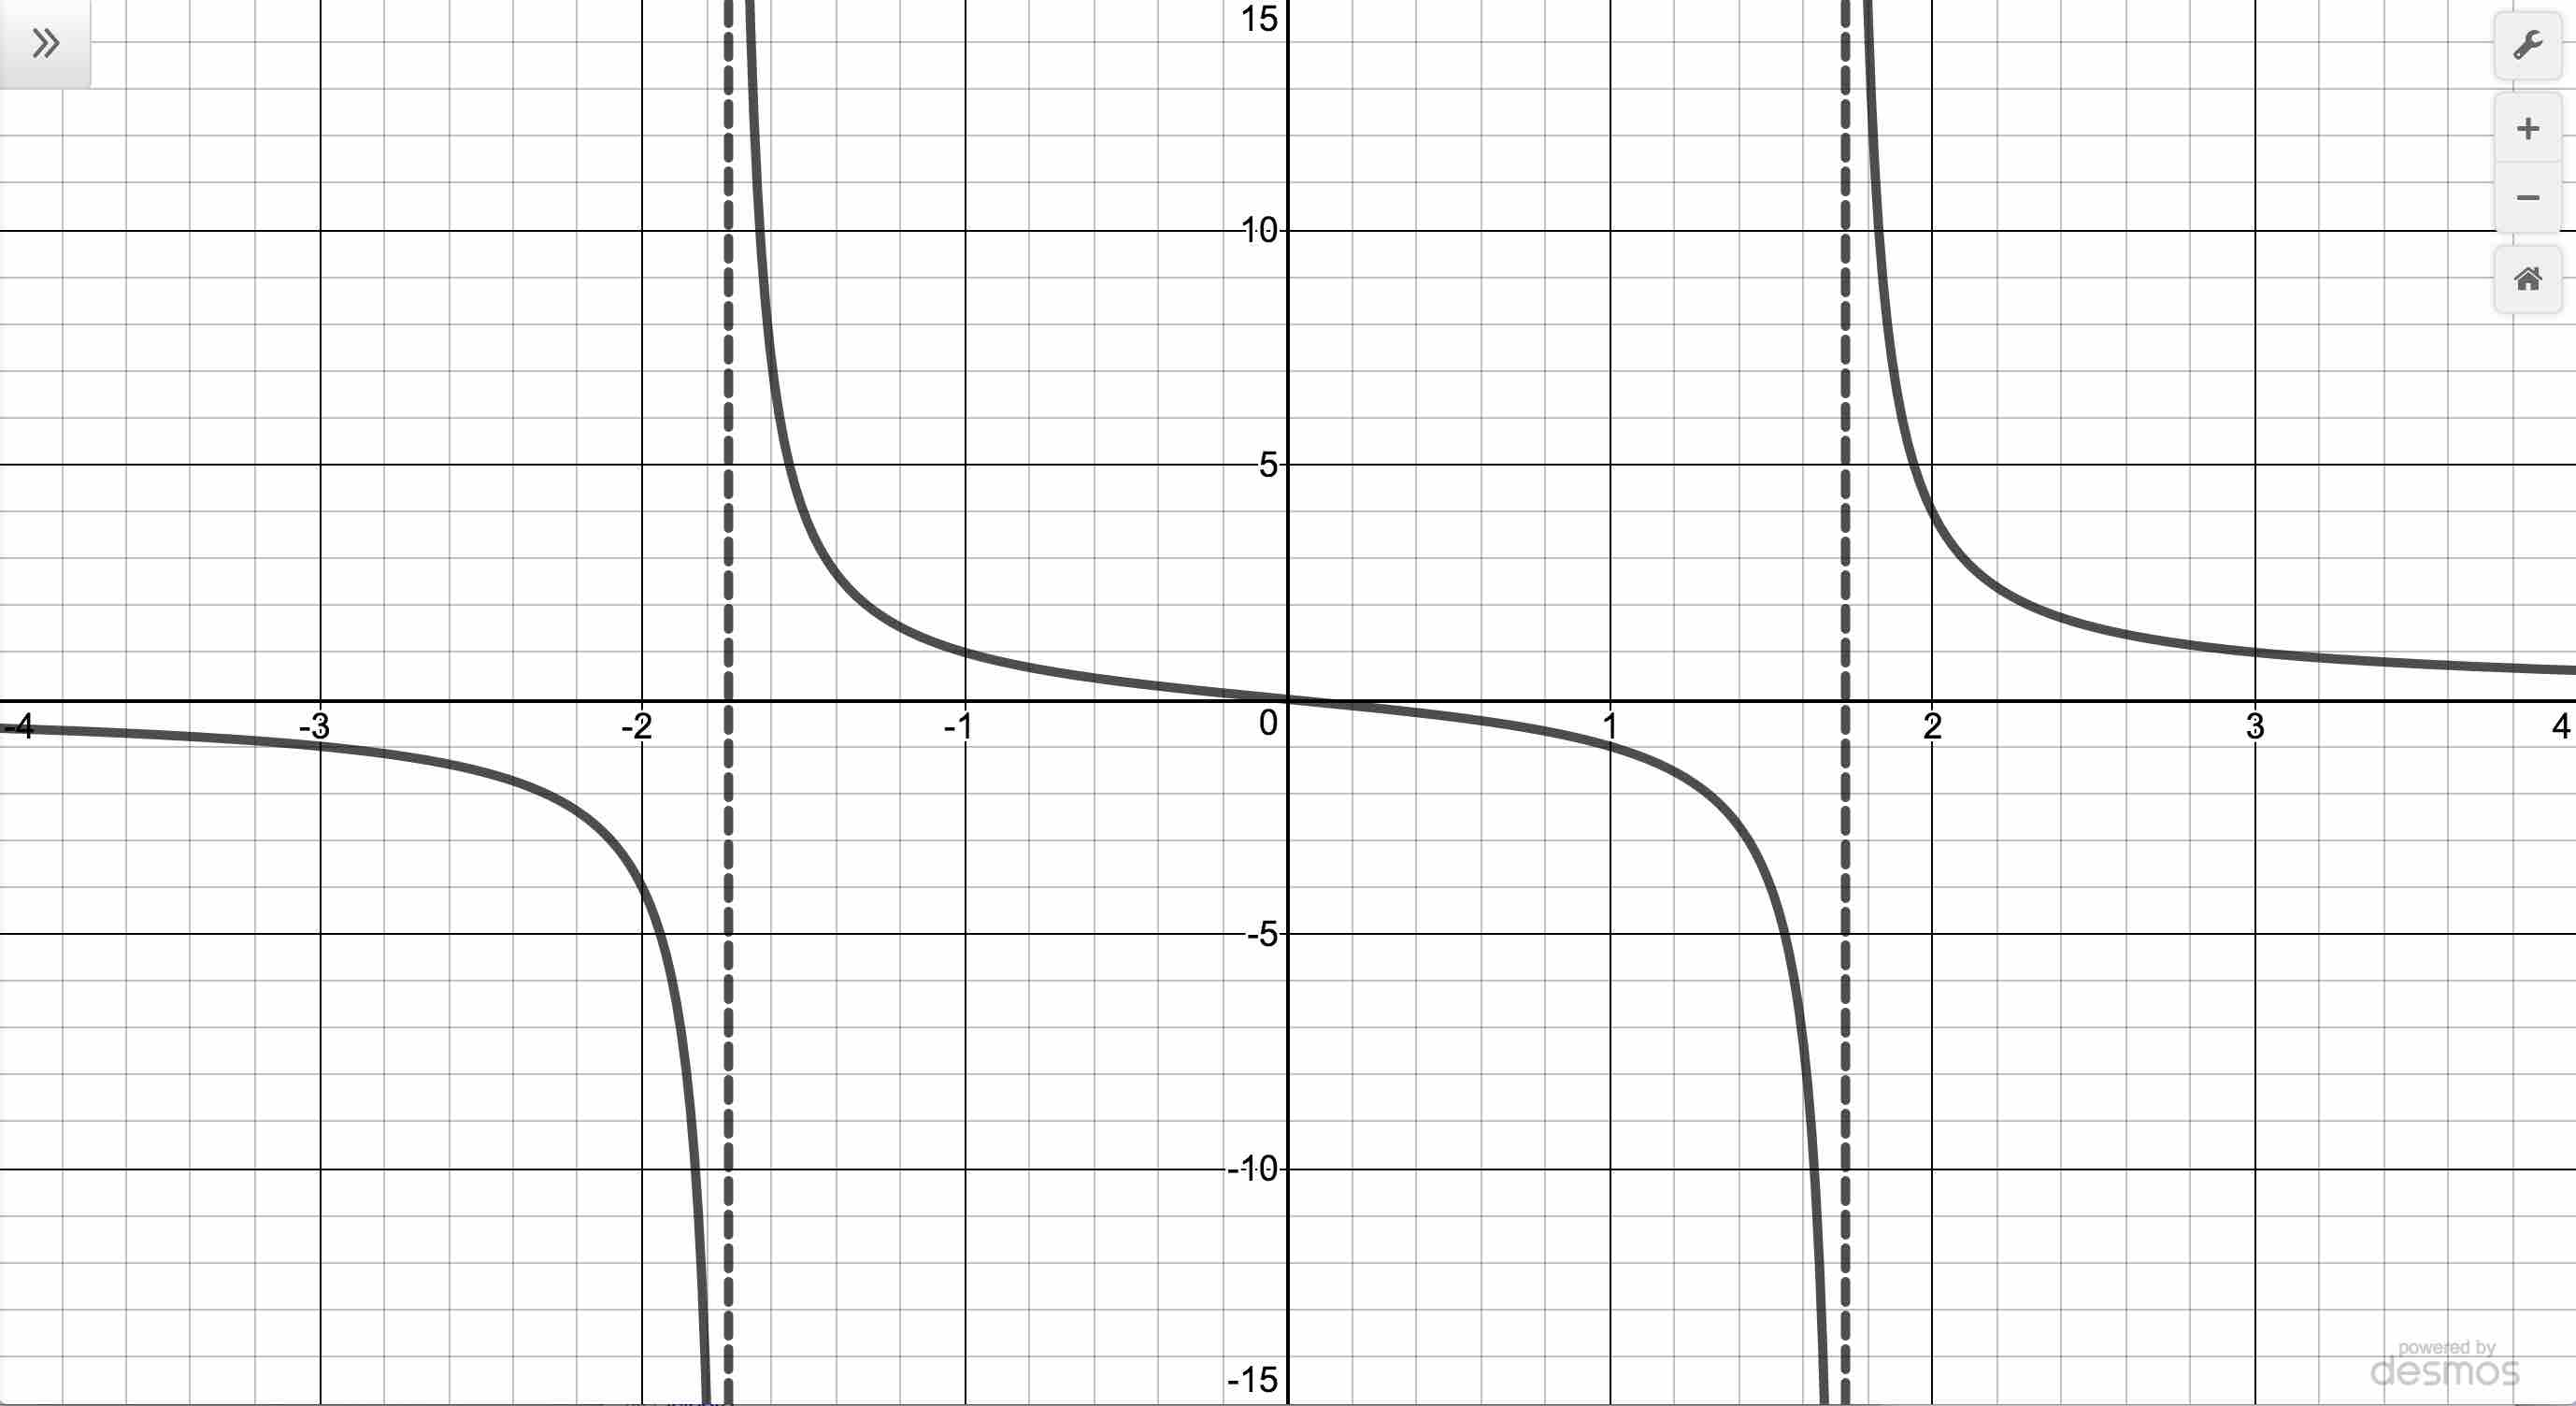
\includegraphics[width=3in]{./IntroRationalGraphics/VAorHoleEx01.jpg} & 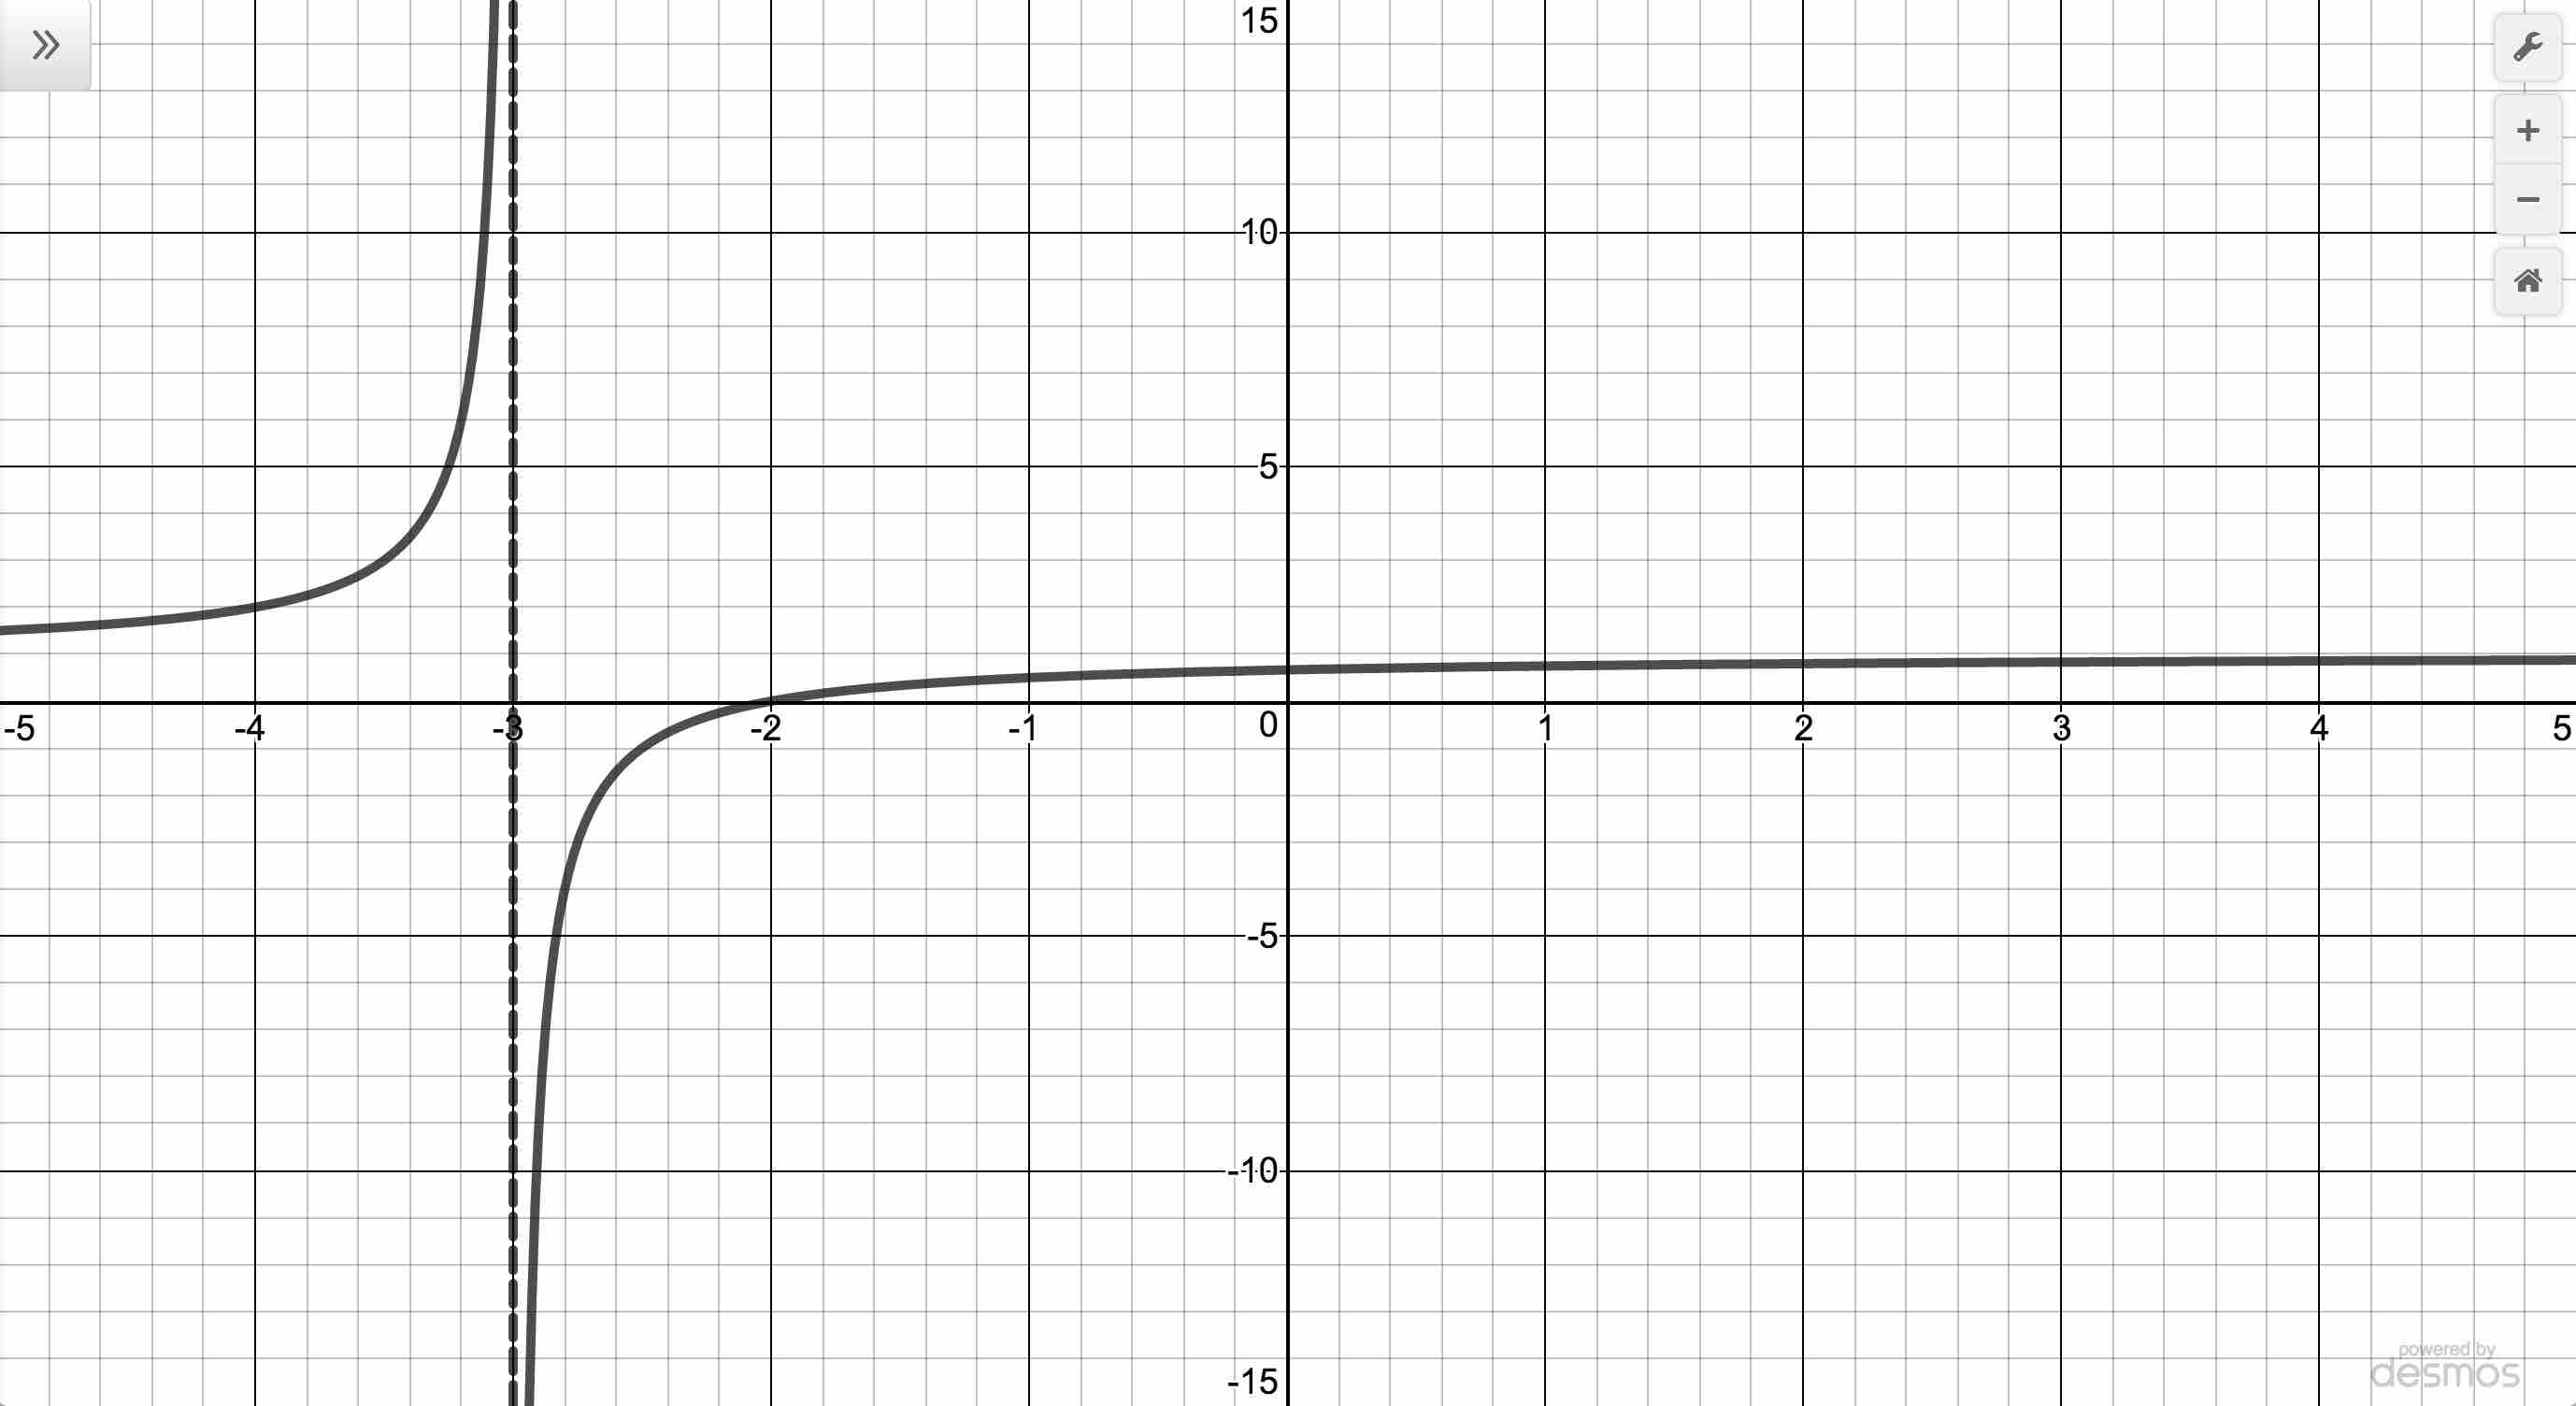
\includegraphics[width=3in]{./IntroRationalGraphics/VAorHoleEx02.jpg} \\

The graph of $y=f(x)$  \hspace{0.75in} & The graph of $y=g(t)$ \\


\end{tabular}
\end{center} 

\item  Setting the denominator of the expression for $h(t)$ to $0$ gives $t^2+9 = 0$, which ahs has no real solutions.  Accordingly, the graph of $y=h(t)$ (at least as much as we can discern from the technology) is devoid of both vertical asymptotes and holes.

\item  Setting the denominator of $r(t)$ to zero gives the equation $t^2+6t+4 = 0$.  We get  the (repeated!) solution $t=-2$.  Simplifying, we see  $r(t) = \frac{t^2-t-6}{t^2+4t+4} = \frac{(t-3)(t+2)}{(t+2)^2} = \frac{t-3}{t+2}$.  Since $t=-2$ continues to produce a $0$ in the denominator of the reduced function, we know $t=-2$ is a vertical asymptote to the graph.  The calculator bears this out, and, moreover, we see that as $t \rightarrow -2^{-}$, $r(t) \rightarrow \infty$ and as $t \rightarrow -2^{+}$, $r(t) \rightarrow -\infty$.


\begin{center}

\begin{tabular}{cc}

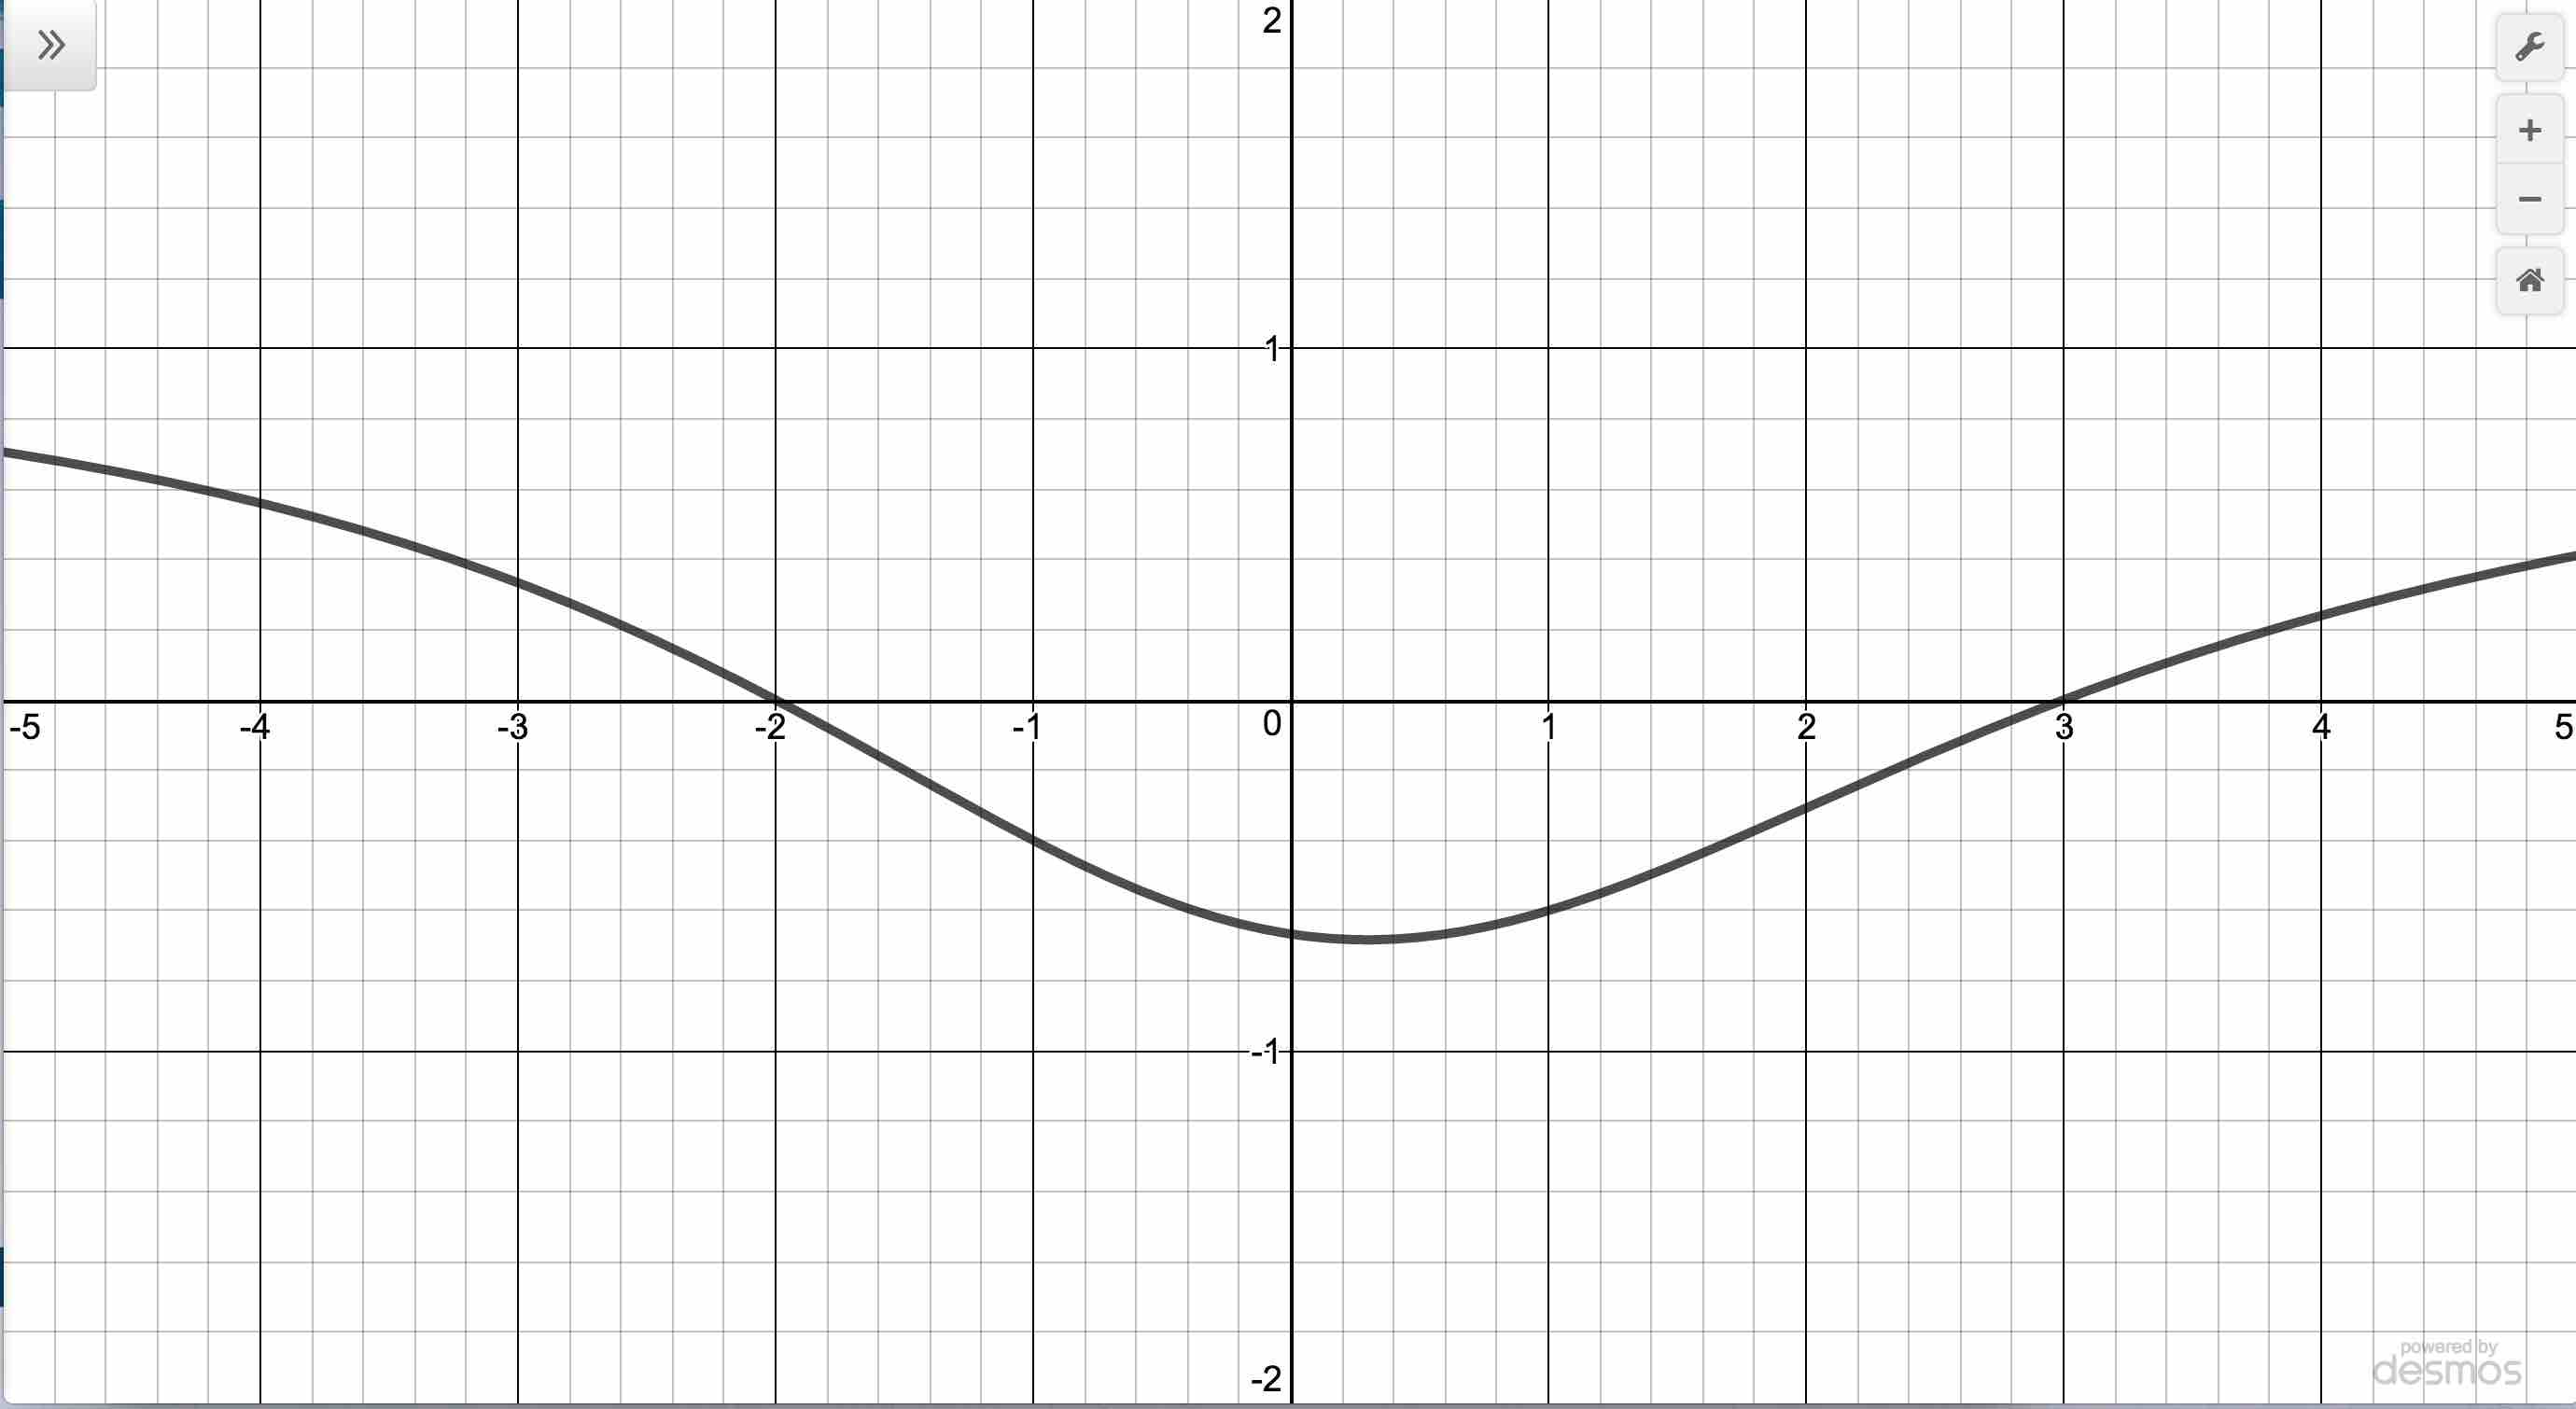
\includegraphics[width=3in]{./IntroRationalGraphics/VAorHoleEx03.jpg} & 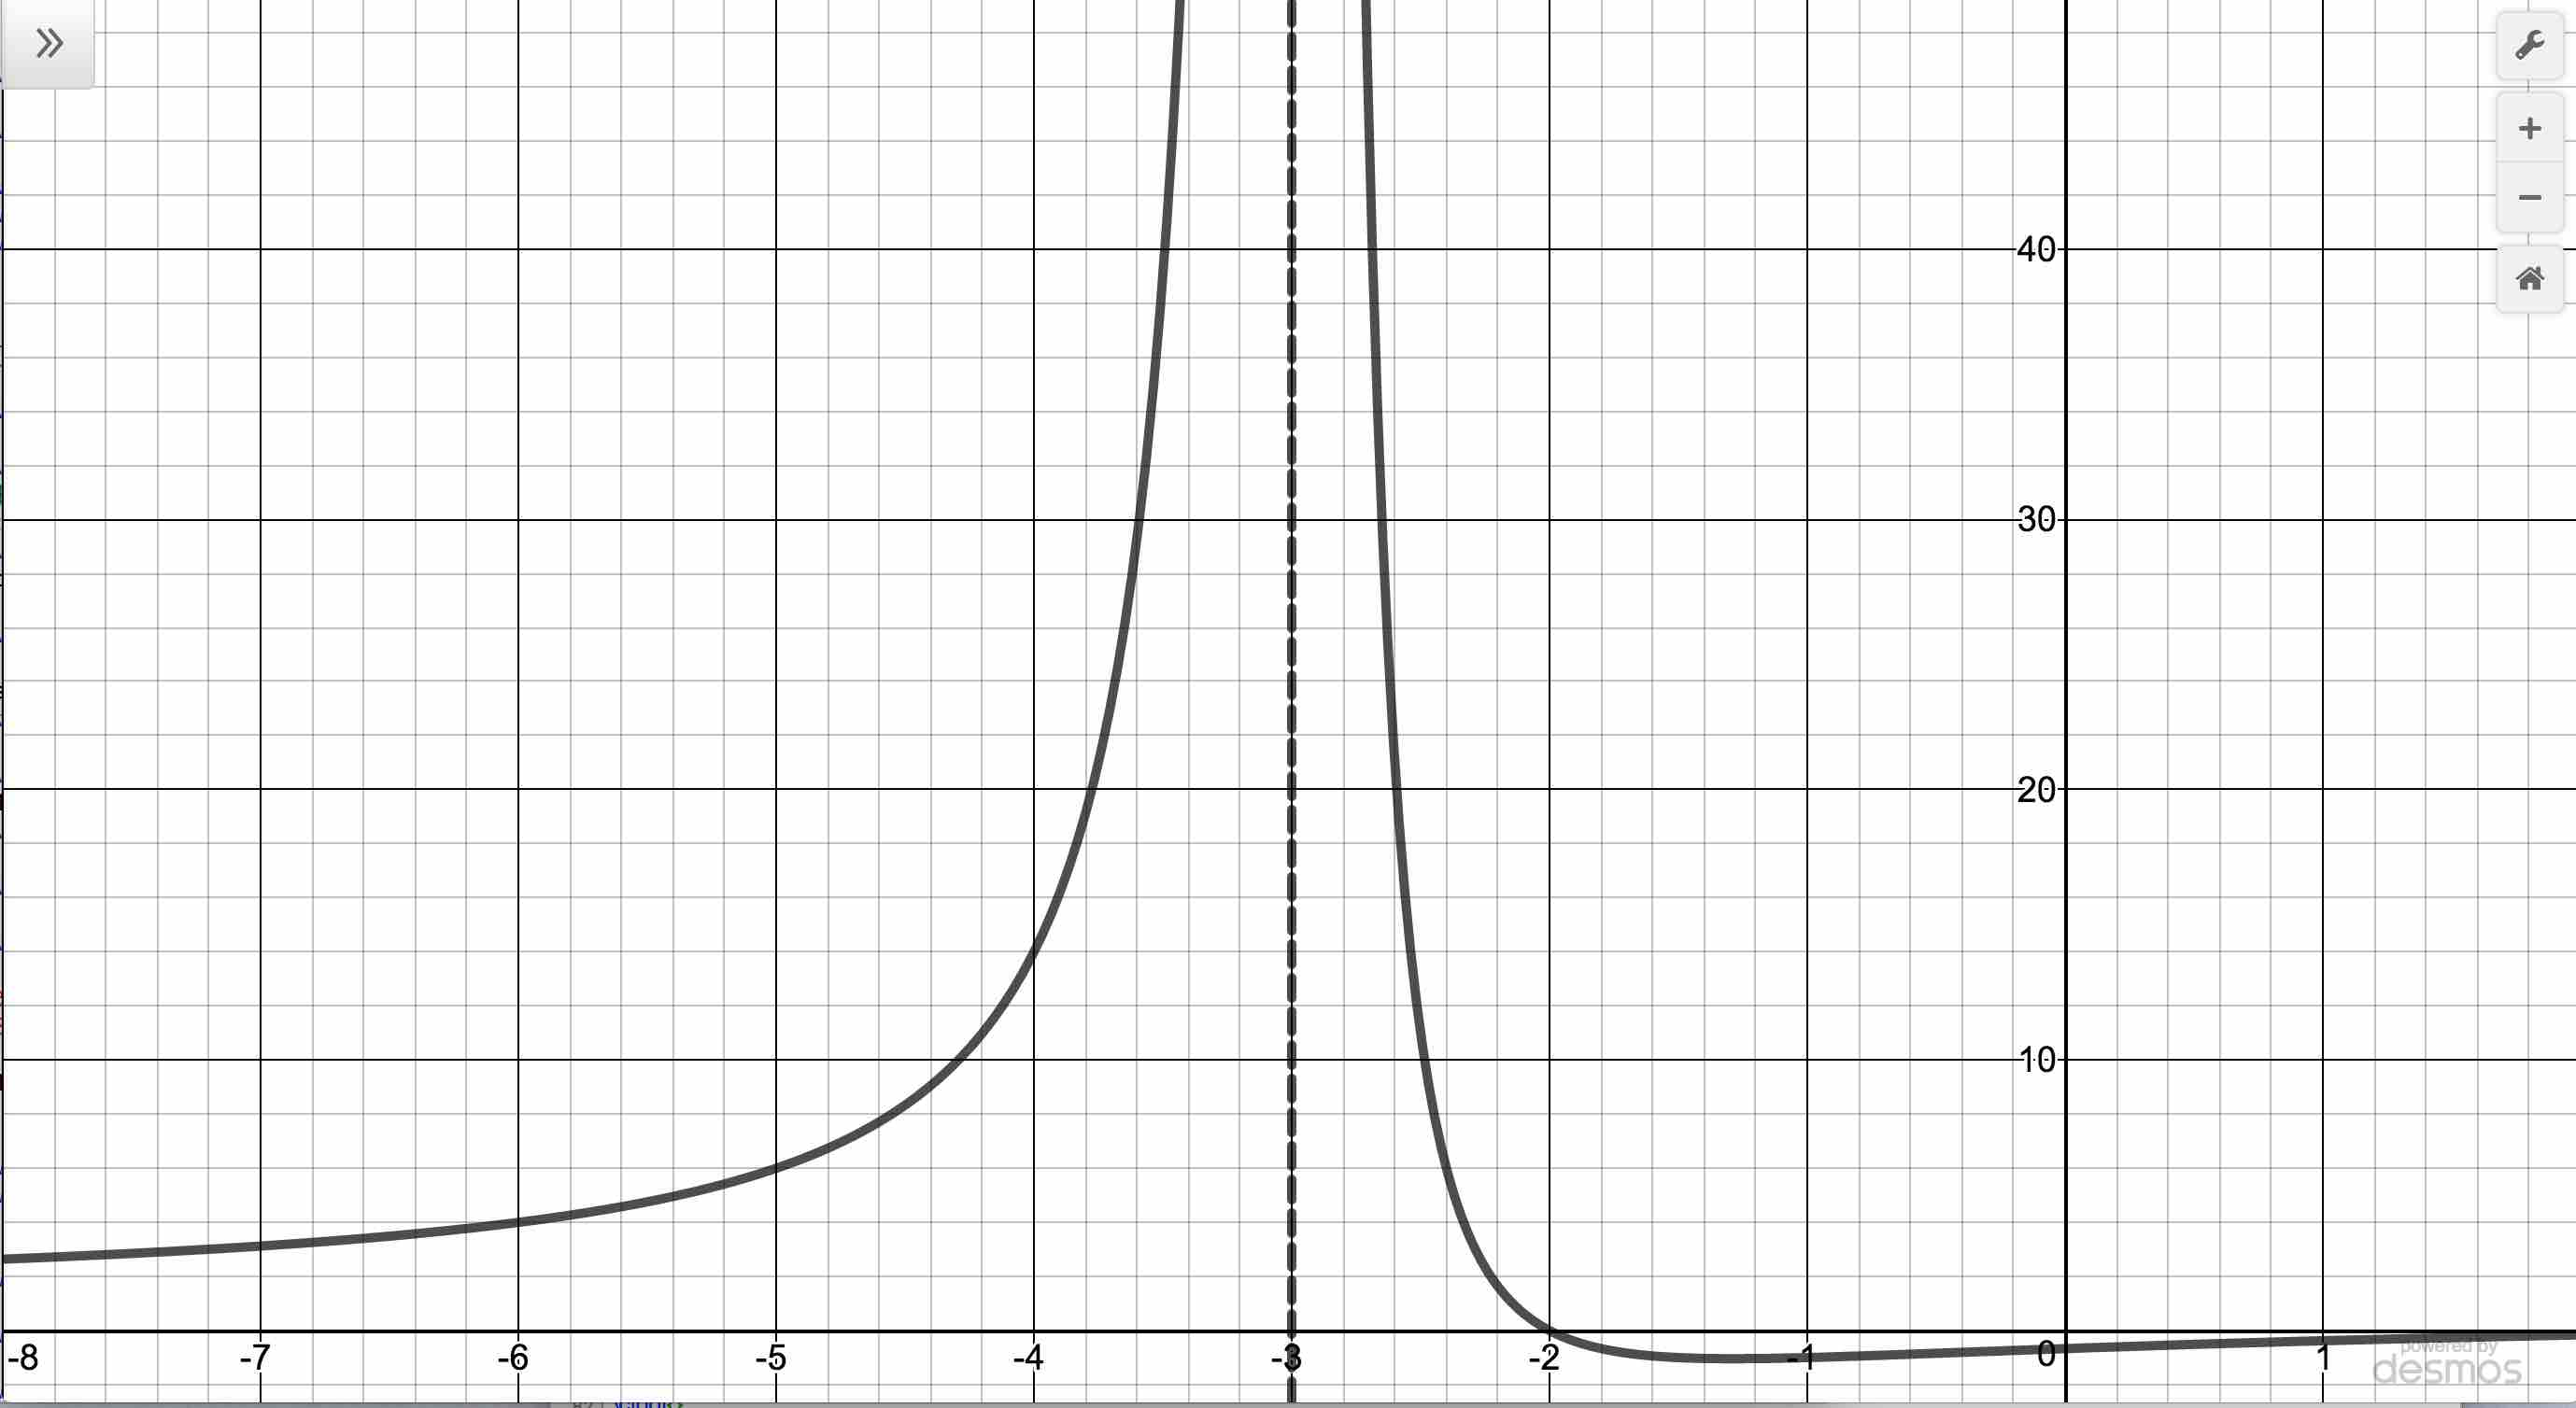
\includegraphics[width=3in]{./IntroRationalGraphics/VAorHoleEx04.jpg} \\

The graph of $y=h(t)$  \hspace{0.75in} & The graph of $y=r(t)$ \\


\end{tabular}
\end{center} 

\end{enumerate}
\qed
\end{ex}

\subsection{End Behavior}
\label{ebrationalsection}

Now that we've thoroughly discussed behavior near values excluded from the domains of rational functions, focus our attention on  end behavior.  We have already seen one example of this in the form of horizontal asymptotes.  Our next example of the section gives us a real-world application of a horizontal asymptote.\footnote{Though the population below is more accurately modeled with the functions in Chapter \ref{ExponentialandLogarithmicFunctions}, we approximate it (using Calculus, of course!) using a rational function.}

\begin{ex}  \label{fluex} The number of students $N(t)$ at local college who have had the flu $t$ months after the semester begins can be modeled by: \[ N(t) = \dfrac{1500t + 50}{3t+1},  \quad t \geq 0.\]

\begin{enumerate}

\item  Find and interpret $N(0)$.

\item  How long will it take until $300$ students will have had the flu?

\item  Use Theorem \ref{linearlaurentlgraphs} to graph $y = N(t)$.  

\item  Find and interpret the behavior of $N$ as $t \rightarrow \infty$.  

\end{enumerate}

{ \bf Solution.}

\begin{enumerate}

\item  Substituting $t=0$ gives $N(0) = \frac{1500(0) + 50}{1+3(0)} = 50$.  Since $t$ represents the number of months since the beginning of the semester, $t=0$ describes the state of the flu outbreak at the beginning of the semester. Hence,  at the beginning of the semester, $50$ students have had the flu.

\item  We set $N(t) = \frac{1500t + 50}{3t+1}  = 300$ and solve.  Clearing denominators gives $1500t + 50 = 300(3t+1)$ from which we get $t = \frac{5}{12}$.  This means it will take $\frac{5}{12}$ months, or about 13 days, for $300$ students to have had the flu.

\item To graph $y = N(t)$, we first use long division to rewrite $N(t) = \frac{-450}{3t+1} + 500$.  From there, we get  \[N(t) =  -\frac{450}{3t+1} + 500  = \frac{-450}{3\left(t + \frac{1}{3}\right)} + 500 = \frac{-150}{t+\frac{1}{3}} + 500\]

Using Theorem \ref{linearlaurentlgraphs}, we start with the graph of $y = \frac{1}{t}$ below on the left and perform the following steps: shift the graph to the left by $\frac{1}{3}$ units, stretch the graph vertically by a factor of $150$, reflect the graph across the $t$-axis, and finally, shift the graph up $500$ units.   As the domain of $N$ is $t \geq 0$, we obtain the graph below on the right.

\[ \begin{array}{ccc}


\begin{mfpic}[15]{-5}{5}{-5}{5}
\axes
\scriptsize
\tlabel[cc](5, -0.5){$t$}
\tlabel[cc](0.5, 5){$y$}
\tlabel[cc](-2, -1.5){$(-1,-1)$}
\tlabel[cc](2, 1.5){$(1,1)$}
\normalsize
\penwd{1.25pt}
\arrow \reverse \arrow \function{-5,-0.2,0.1}{1/x}
\arrow \reverse \arrow \function{0.2,5,0.1}{1/x}
\point[4pt]{(-1,-1), (1,1)}
\tcaption{\scriptsize $y =  \frac{1}{t}$}
\end{mfpic}


&
\stackrel{\text{Theorem \ref{linearlaurentlgraphs}}}{\xrightarrow{\hspace{1.5in}}}

&

\begin{mfpic}[15]{-1}{9}{-1}{9}
\axes
\dashed \polyline{(-1,5), (9,5)}
\scriptsize
\tlabel[cc](9, -0.5){$t$}
\tlabel[cc](0.5, 9){$y$}
\tlabel[cc](7, 5.5){$y = 500$}
\tlabel[cc](-1, 0.5){$(0,50)$}
\tlabel[cc](1.75, 3.25){$\left(\frac{2}{3},350 \right)$}
\normalsize
\penwd{1.25pt}
\arrow \function{0,9,0.1}{5 - (1.5/(x+1/3))}
\point[4pt]{(0,0.5), (0.6666,3.5)}
\tcaption{\scriptsize $y=N(t)$}
\end{mfpic}
 \\

 \text{\scriptsize  $(-1,1)$ , $(1,1)$,  HA: $y=0$} & & \text{\scriptsize $\left(\frac{2}{3},350 \right)$, HA: $y = 500$  } \\
 
 \end{array} \]


  
\item  From the graph, we see as $t \rightarrow \infty$, $N(t) \rightarrow 500$. (More specifically, $500^{-}$.)  This means as time goes by, only a total of 500 students will have ever had the flu. \qed

\end{enumerate}

\end{ex}
 
 We determined the horizontal asymptote to the graph of $y = N(t)$ in Example \ref{fluex} by rewriting $N(t)$ into a form compatible with Theorem  \ref{linearlaurentlgraphs}, and while there is nothing wrong with this approach, it will simply not work for general rational functions which cannot be rewritten this way.  To that end, we revisit this problem using Theorem \ref{EBPolynomials} from Section \ref{GraphsofPolynomials}.  The end behavior of the numerator of $N(t) = \frac{1500t + 50}{3t+1}$ is determined by its leading term,  $1500t$,  and the end behavior of the denominator is likewise determined  by its leading term, $3t$.  Hence, as $t \rightarrow \pm \infty$, 
 
 \[ N(t) = \dfrac{1500t + 50}{3t+1} \approx \dfrac{1500t}{3t} = 500.\]
 
Hence as $t \rightarrow \pm \infty$, $y = N(t) \rightarrow 500$, producing the horizontal asymptote $y = 500$.  This same reasoning can be used in general to argue the following theorem.

\smallskip
\colorbox{ResultColor}{\bbm

\begin{thm} \index{asymptote ! horizontal ! location of}\index{horizontal asymptote ! location of}\textbf{Location of Horizontal Asymptotes:}\label{hathm} Suppose $r$ is a rational function and $r(x) = \frac{p(x)}{q(x)}$, where $p$ and $q$ are polynomial functions with leading coefficients $a$ and $b$, respectively. 

\begin{itemize}

\item  If the degree of $p(x)$ is the same as the degree of $q(x)$, then $y=\frac{a}{b}$ is the\footnote{The use of the definite article will be justified momentarily.} horizontal asymptote of the graph of $y=r(x)$.

\item  If the degree of $p(x)$ is less than the degree of $q(x)$, then $y=0$ is the horizontal asymptote of the graph of $y=r(x)$.

\item  If the degree of $p(x)$ is greater than the degree of $q(x)$, then the graph of $y=r(x)$ has no horizontal asymptotes.


\end{itemize}
\end{thm}
\ebm}
\smallskip

\end{ex}

So see why Theorem \ref{hathm} works, suppose $r(x) = \frac{p(x)}{q(x)}$ where $a$ is the leading coefficient of $p(x)$ and $b$ is the leading coefficient of $q(x)$. As $x \rightarrow \pm \infty$,  Theorem \ref{EBPolynomials} gives $r(x) \approx \frac{ax^n}{bx^m}$, where $n$ and $m$ are the degrees of $p(x)$ and $q(x)$, respectively. 

If the degree of $p(x)$ and the degree of $q(x)$ are the same, then $n=m$ so that $r(x) \approx \frac{ax^n}{bx^n} = \frac{a}{b}$, which means $y=\frac{a}{b}$ is the horizontal asymptote in this case.  

If the degree of $p(x)$ is less than the degree of $q(x)$, then $n < m$, so $m-n$ is a positive number, and hence, $r(x) \approx  \frac{ax^n}{bx^m}  = \frac{a}{bx^{m-n}} \rightarrow 0$.   As $x \rightarrow \pm \infty$, $r(x)$ is more or less a fraction with a constant numerator, $a$, but a denominator which is unbounded. Hence, $r(x) \rightarrow 0$ producing the horizontal asymptote $y = 0$.   

If the degree of $p(x)$ is greater than the degree of $q(x)$, then $n > m$, and hence $n-m$ is a positive number and $r(x) \approx  \frac{ax^n}{bx^m}  = \frac{ax^{n-m}}{ b}$, which is a monomial function from Section \ref{GraphsofPolynomials}.  As such, $r$ becomes unbounded as $x \rightarrow \pm \infty$.

Note that in the two cases which produce horizontal asymptotes, the behavior of $r$ is identical as $x \rightarrow \infty$ and $x \rightarrow -\infty$.  Hence, if the graph of a rational function has a horizontal asymptote, there is only one.\footnote{We will (first) encounter functions with more than one horizontal asymptote in Chapter \ref{RootRadicalFunctions}.} 

We put Theorem \ref{hathm}  to good use in the following example.
 
\begin{ex} \label{haexample} For each function below:

\begin{itemize}

\item use Theorem \ref{EBPolynomials} to  analytically determine the horizontal asymptotes to the graph, if any.

\item check your answers Theorem \ref{hathm} and a graphing utility.   

\item describe the end behavior of the graph using proper notation.

\item  investigate any apparent symmetry of the graph about the $y$-axis or origin.

\end{itemize}

\begin{multicols}{2}
\begin{enumerate}

\item $F(s) = \dfrac{5s}{s^2+1}$  \vphantom{ $g(x) = \dfrac{x^2-4}{x+1}$}

\item  $g(x) = \dfrac{x^2-4}{x+1}$ 

\setcounter{HW}{\value{enumi}}
\end{enumerate}
\end{multicols}

\begin{multicols}{2}
\begin{enumerate}
\setcounter{enumi}{\value{HW}}


\item  $h(t) = \dfrac{6t^3-3t+1}{5-2t^3}$

\item  $r(x) = 2 - \dfrac{3x^2}{1-x^2}$ \vphantom{ $h(t) = \dfrac{6t^3-3t+1}{5-2t^3}$}

\setcounter{HW}{\value{enumi}}
\end{enumerate}
\end{multicols}


{ \bf Solution.}

\begin{enumerate}

\item  Using  Theorem \ref{EBPolynomials}, we get as $s \pm \infty$, $F(s) = \frac{5s}{s^2+1}  \approx \frac{5s}{s^2} = \frac{5}{s}$.  Hence, as $s \rightarrow \infty$, $F(s) \rightarrow 0$, so $y = 0$ is a horizontal asymptote to the graph of $y = F(s)$.  To check, we note that since the degree of the  numerator of $F(s)$,  $1$, is less than the degree of the denominator, $2$ Theorem \ref{hathm} gives  $y=0$ is the horizontal asymptote.  Graphically, we see as  $s \rightarrow  \pm \infty$, $F(s) \rightarrow 0$.  More specifically, as $s \rightarrow -\infty$, $F(s)  \rightarrow 0^{-}$ and as $s \rightarrow \infty$, $F(s)  \rightarrow 0^{+}$.  As a side note, the graph of $F$ appears to be symmetric about the origin.  Indeed, $F(-s) = \frac{5(-s)}{(-s)^2+1} = -\frac{5s}{s^2+1}$ proving $F$ is odd.

\item  As $x \rightarrow \pm \infty$, $g(x) = \frac{x^2-4}{x+1} \approx \frac{x^2}{x} = x$, and while $y = x$ is a line, it is not a horizontal line.  Hence, we conclude the graph of $y = g(x)$ has no horizontal asymptotes.  Sure enough,  Theorem \ref{hathm} supports this since the degree of the numerator of $g(x)$ is $2$ which is greater than the degree of the denominator, $1$.     By, there is no horizontal asymptote.  From the graph, we see that the graph of $y=g(x)$ doesn't appear to level off to a constant value, so there is no horizontal asymptote.\footnote{Sit tight!  We'll revisit this function and its end behavior shortly.}

\begin{center}
\begin{tabular}{cc}

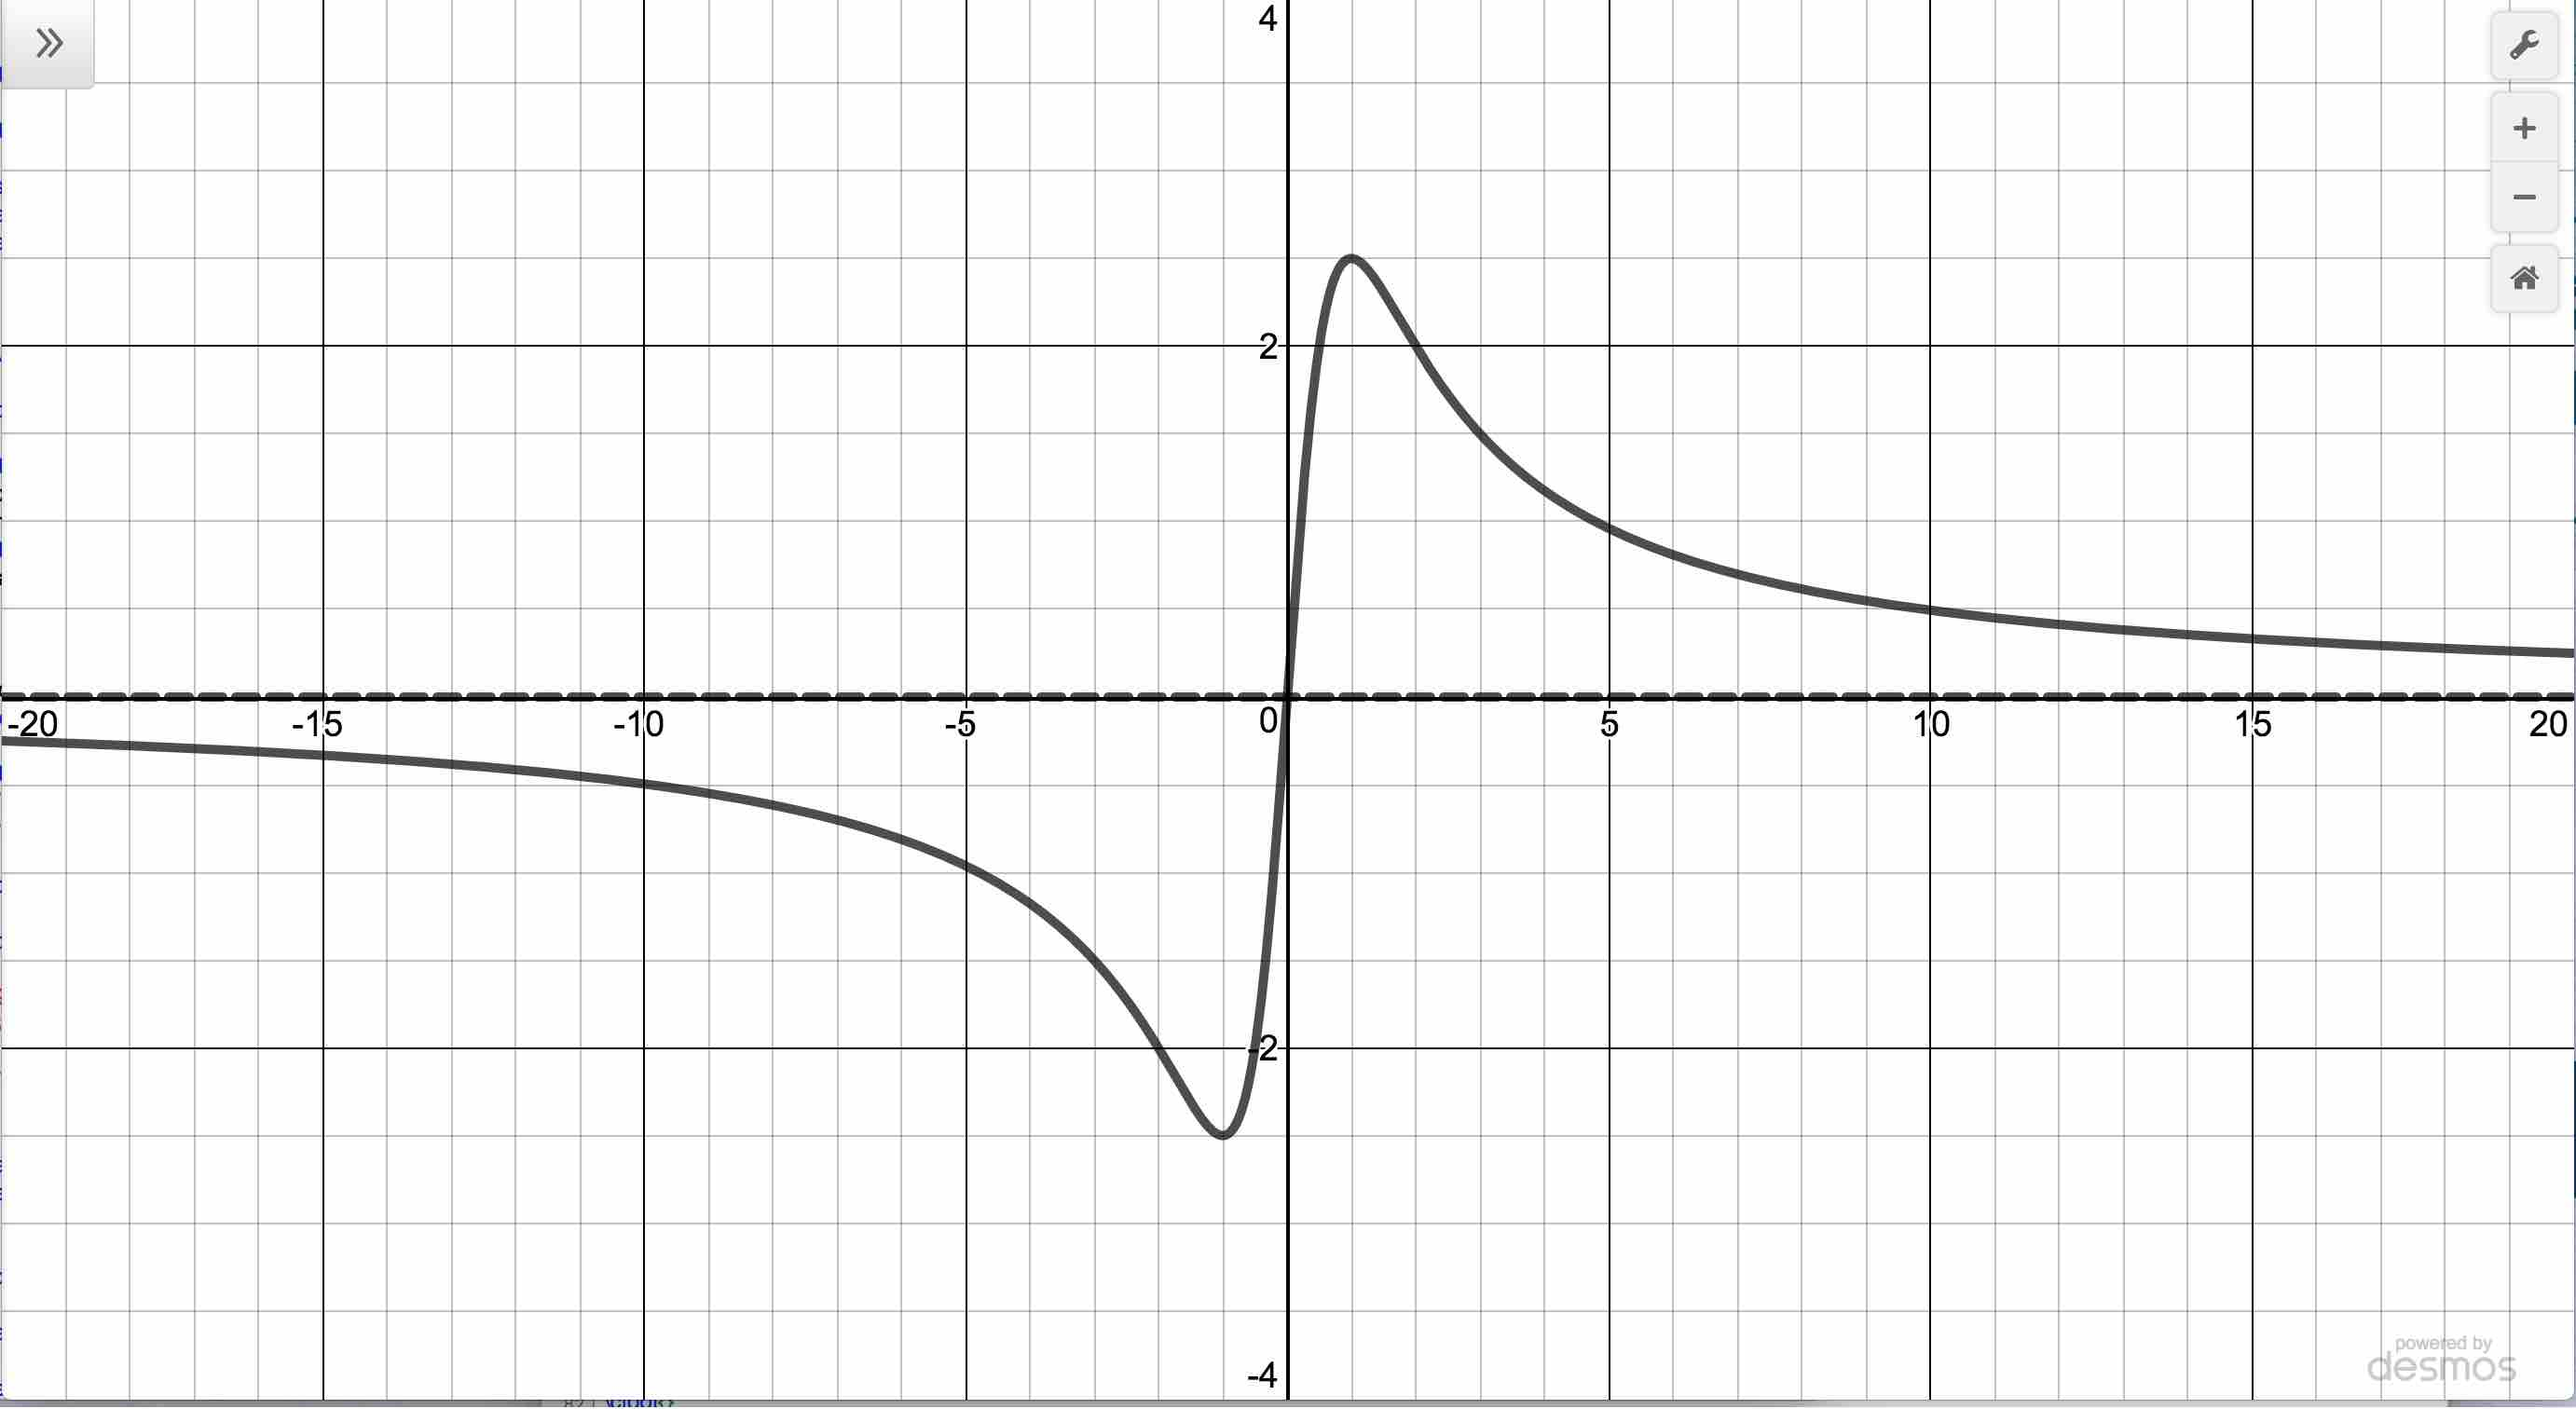
\includegraphics[width=3in]{./IntroRationalGraphics/HAEx01.jpg}  & 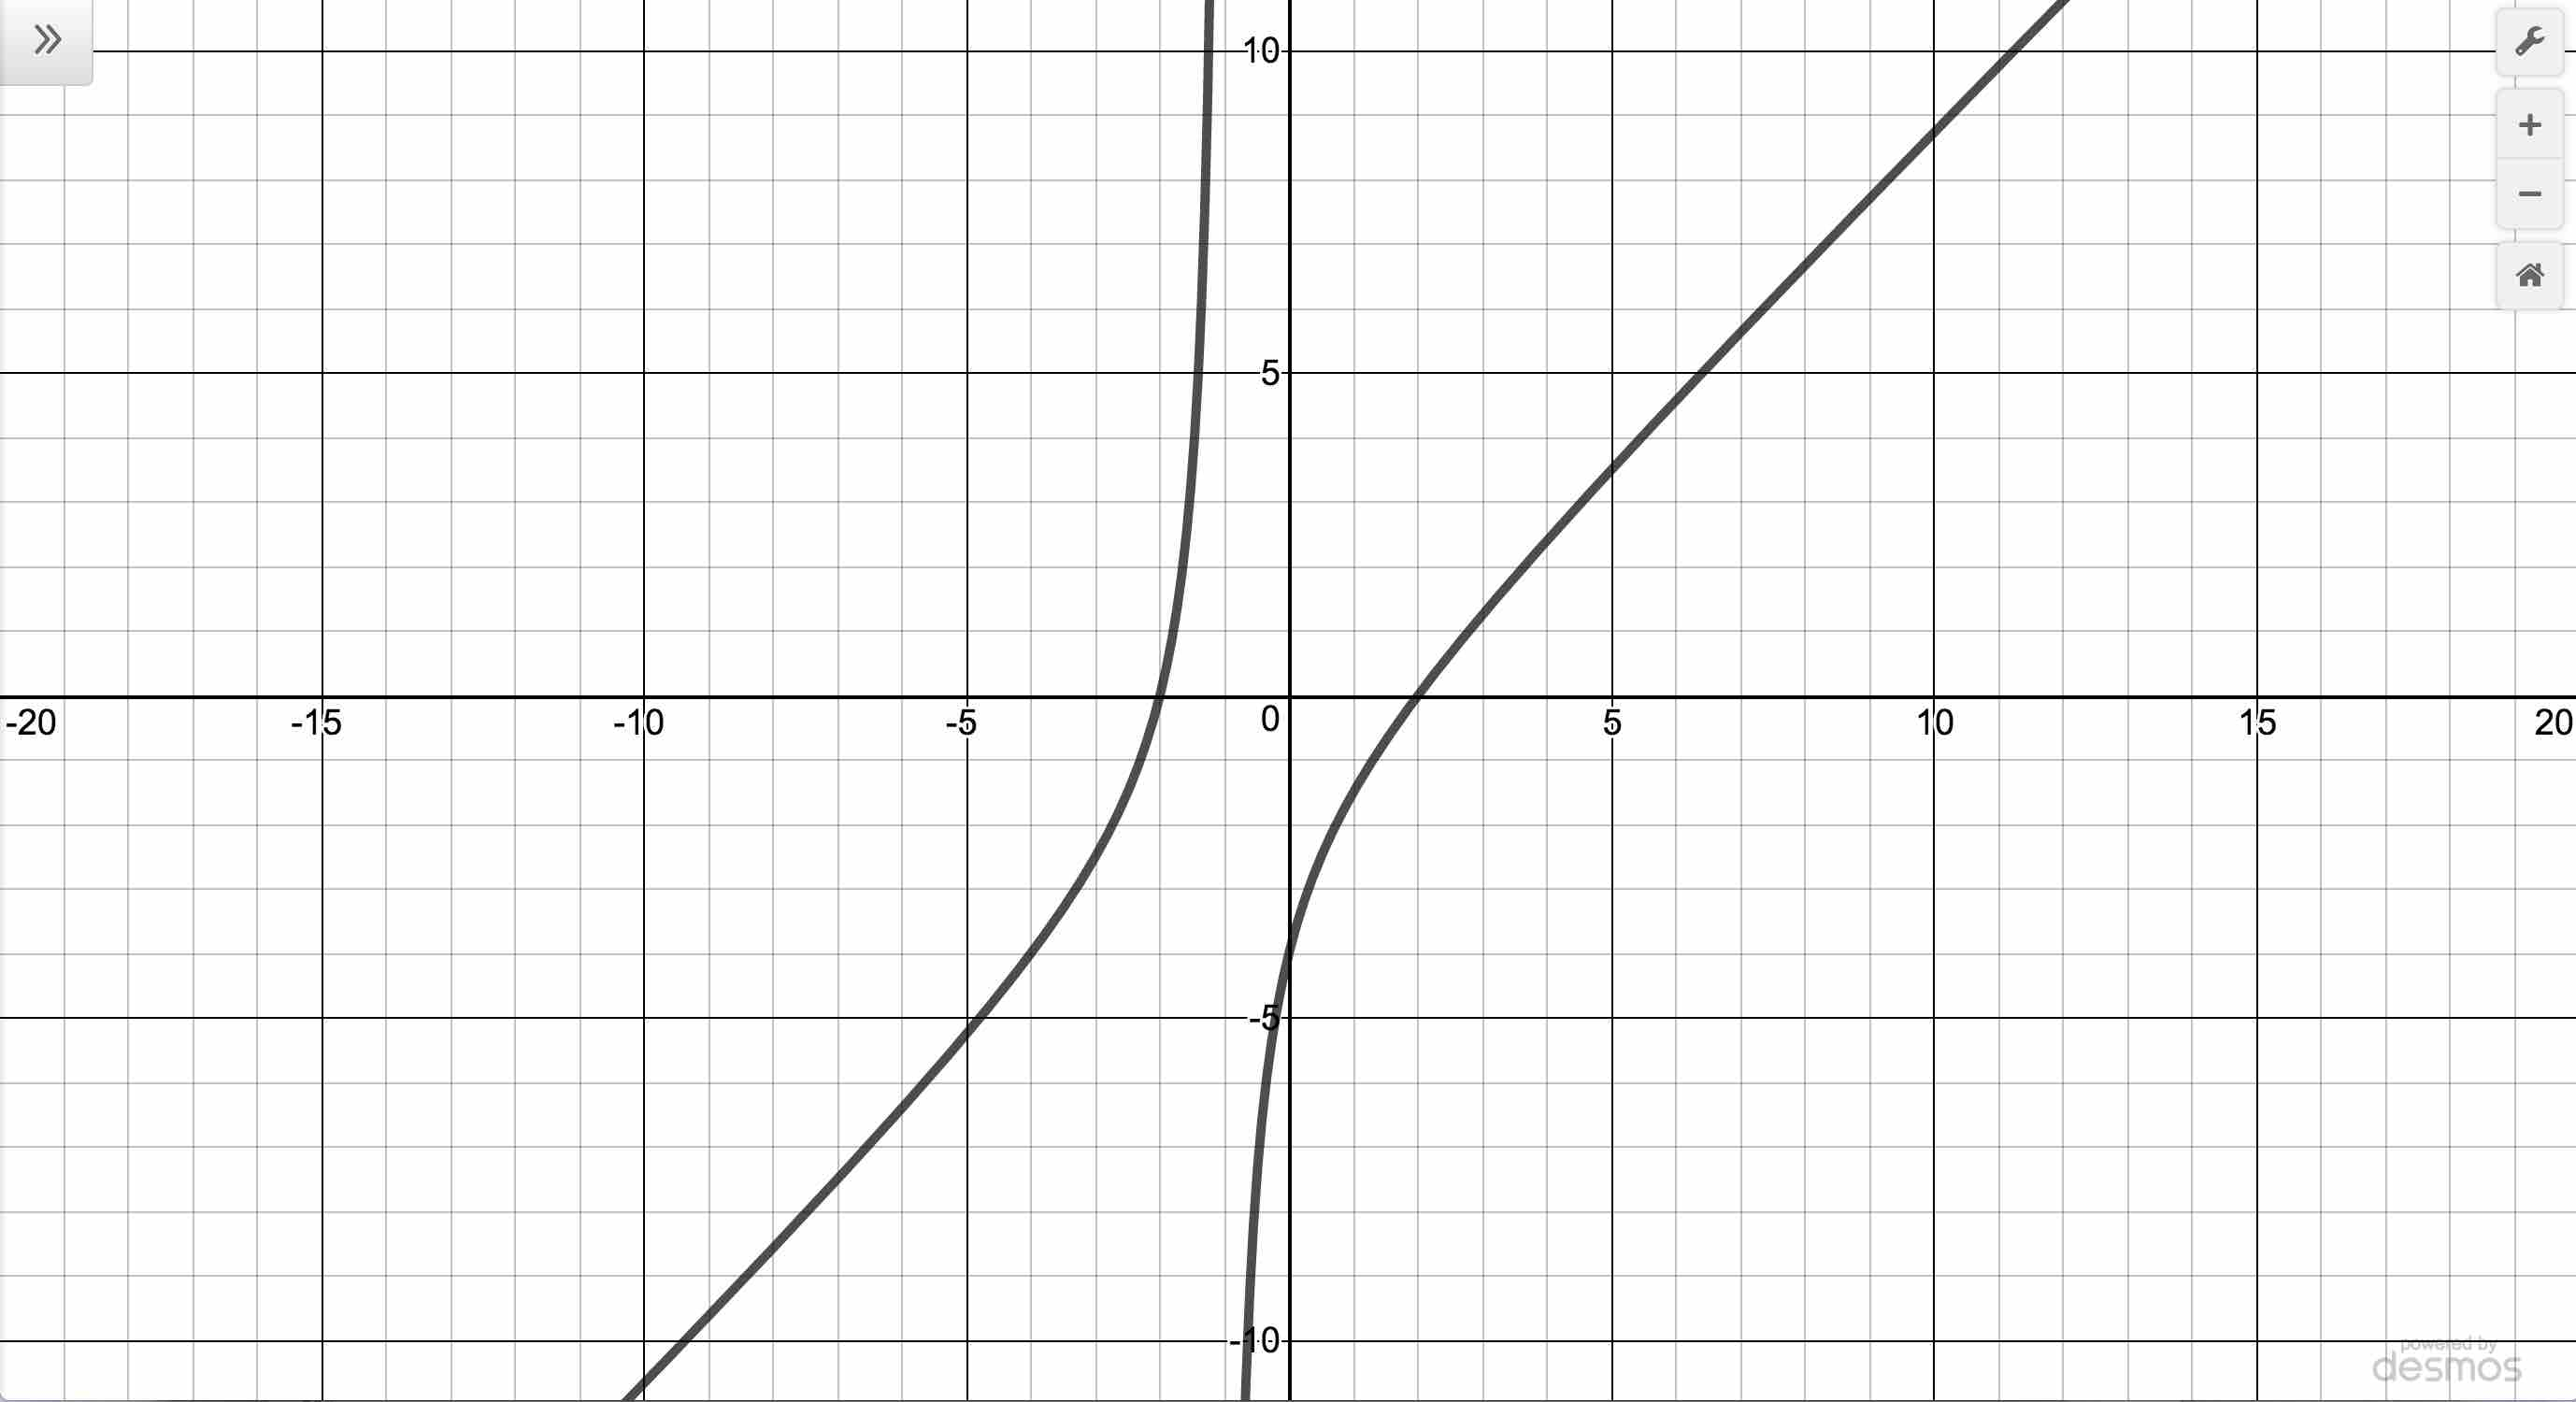
\includegraphics[width=3in]{./IntroRationalGraphics/HAEx02.jpg} \\
The graph of $y=F(s)$  & The graph of $y=g(x)$ \\


\end{tabular}
\end{center} 

\item  We have $h(t) = \frac{6t^3-3t+1}{5-2t^3} \approx  \frac{6t^3}{-2t^3} = -3$ as $t \rightarrow \pm \infty$, indicating a horizontal asymptote $y = -3$.  Sure enough, since the degrees of the numerator and denominator of $h(t)$ are both three,  Theorem \ref{hathm} tells us $y = \frac{6}{-2} = -3$ is the horizontal asymptote.  We see from the graph of $y = h(t)$ that as $t \rightarrow -\infty$, $h(t) \rightarrow -3^{+}$, and as $t \rightarrow \infty$, $h(t) \rightarrow -3^{-}$.

\item  If we apply Theorem \ref{EBPolynomials} to the term  $\frac{3x^2}{1-x^2}$ in the expression for $r(x)$, we find   $\frac{3x^2}{1-x^2} \approx \frac{3x^2}{-x^2} = -3$ as $x \rightarrow \pm \infty$.  It  seems reasonable to conclude, then, that  $r(x) = 2 - \frac{3x^2}{1-x^2} \approx 2 - (-3) = 5$ so $y = 5$ is our horizontal asymptote.  In order to use Theorem \ref{hathm} as stated, however, we need to rewrite the expression $r(x)$ with a single denominator:  $r(x) = 2 - \frac{3x^2}{1-x^2} = \frac{2(1-x^2) - 3x^2}{1-x^2} = \frac{2-5x^2}{1-x^2}$.  Now we apply Theorem \ref{hathm}  and note since the numerator and denominator have the same degree, we are guaranteed the horizontal asymptote is $y = \frac{-5}{-1} = 5$.  These calculations are borne out graphically below where it appears as if as $x \rightarrow \pm \infty$, $r(x) \rightarrow 5^{+}$.  As a final note, the graph of $r$ appears to be symmetric about the $y$ axis.  We find $r(-x) = 2 - \frac{3(-x)^2}{1-(-x)^2} = 2 - \frac{3x^2}{1-x^2} = r(x)$, proving $r$ is even.

\begin{center}
\begin{tabular}{cc}

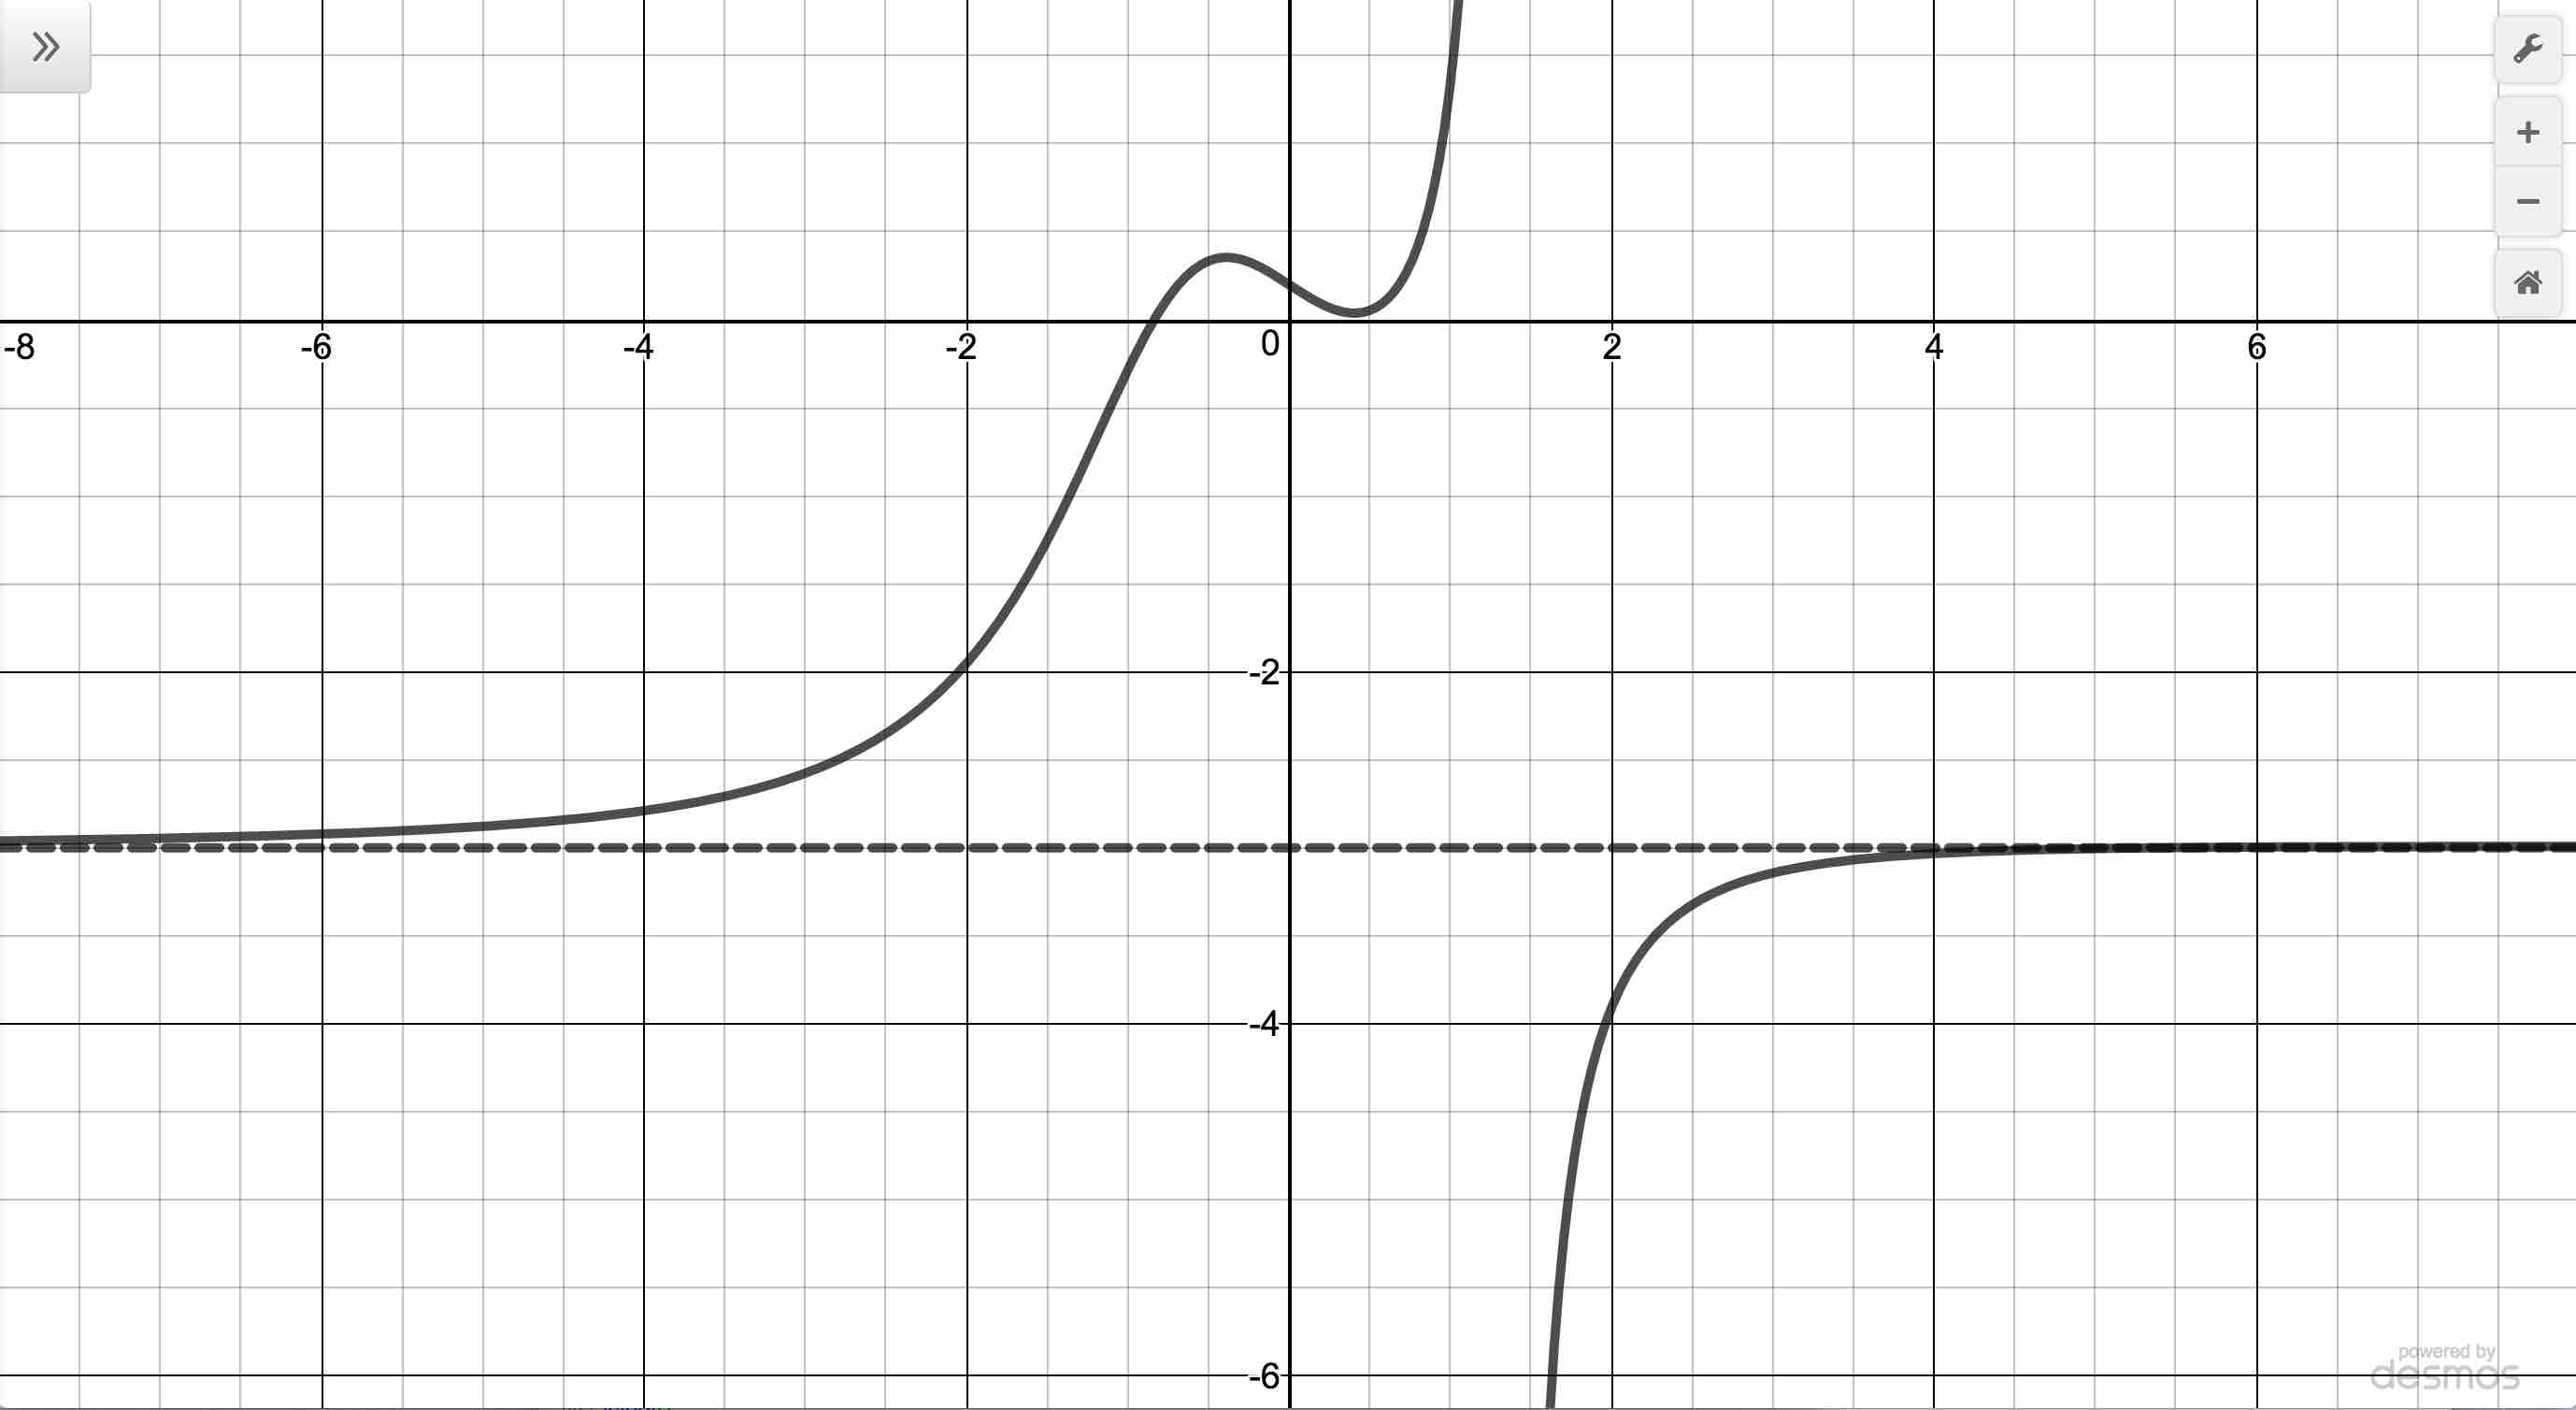
\includegraphics[width=3in]{./IntroRationalGraphics/HAEx03.jpg}  & 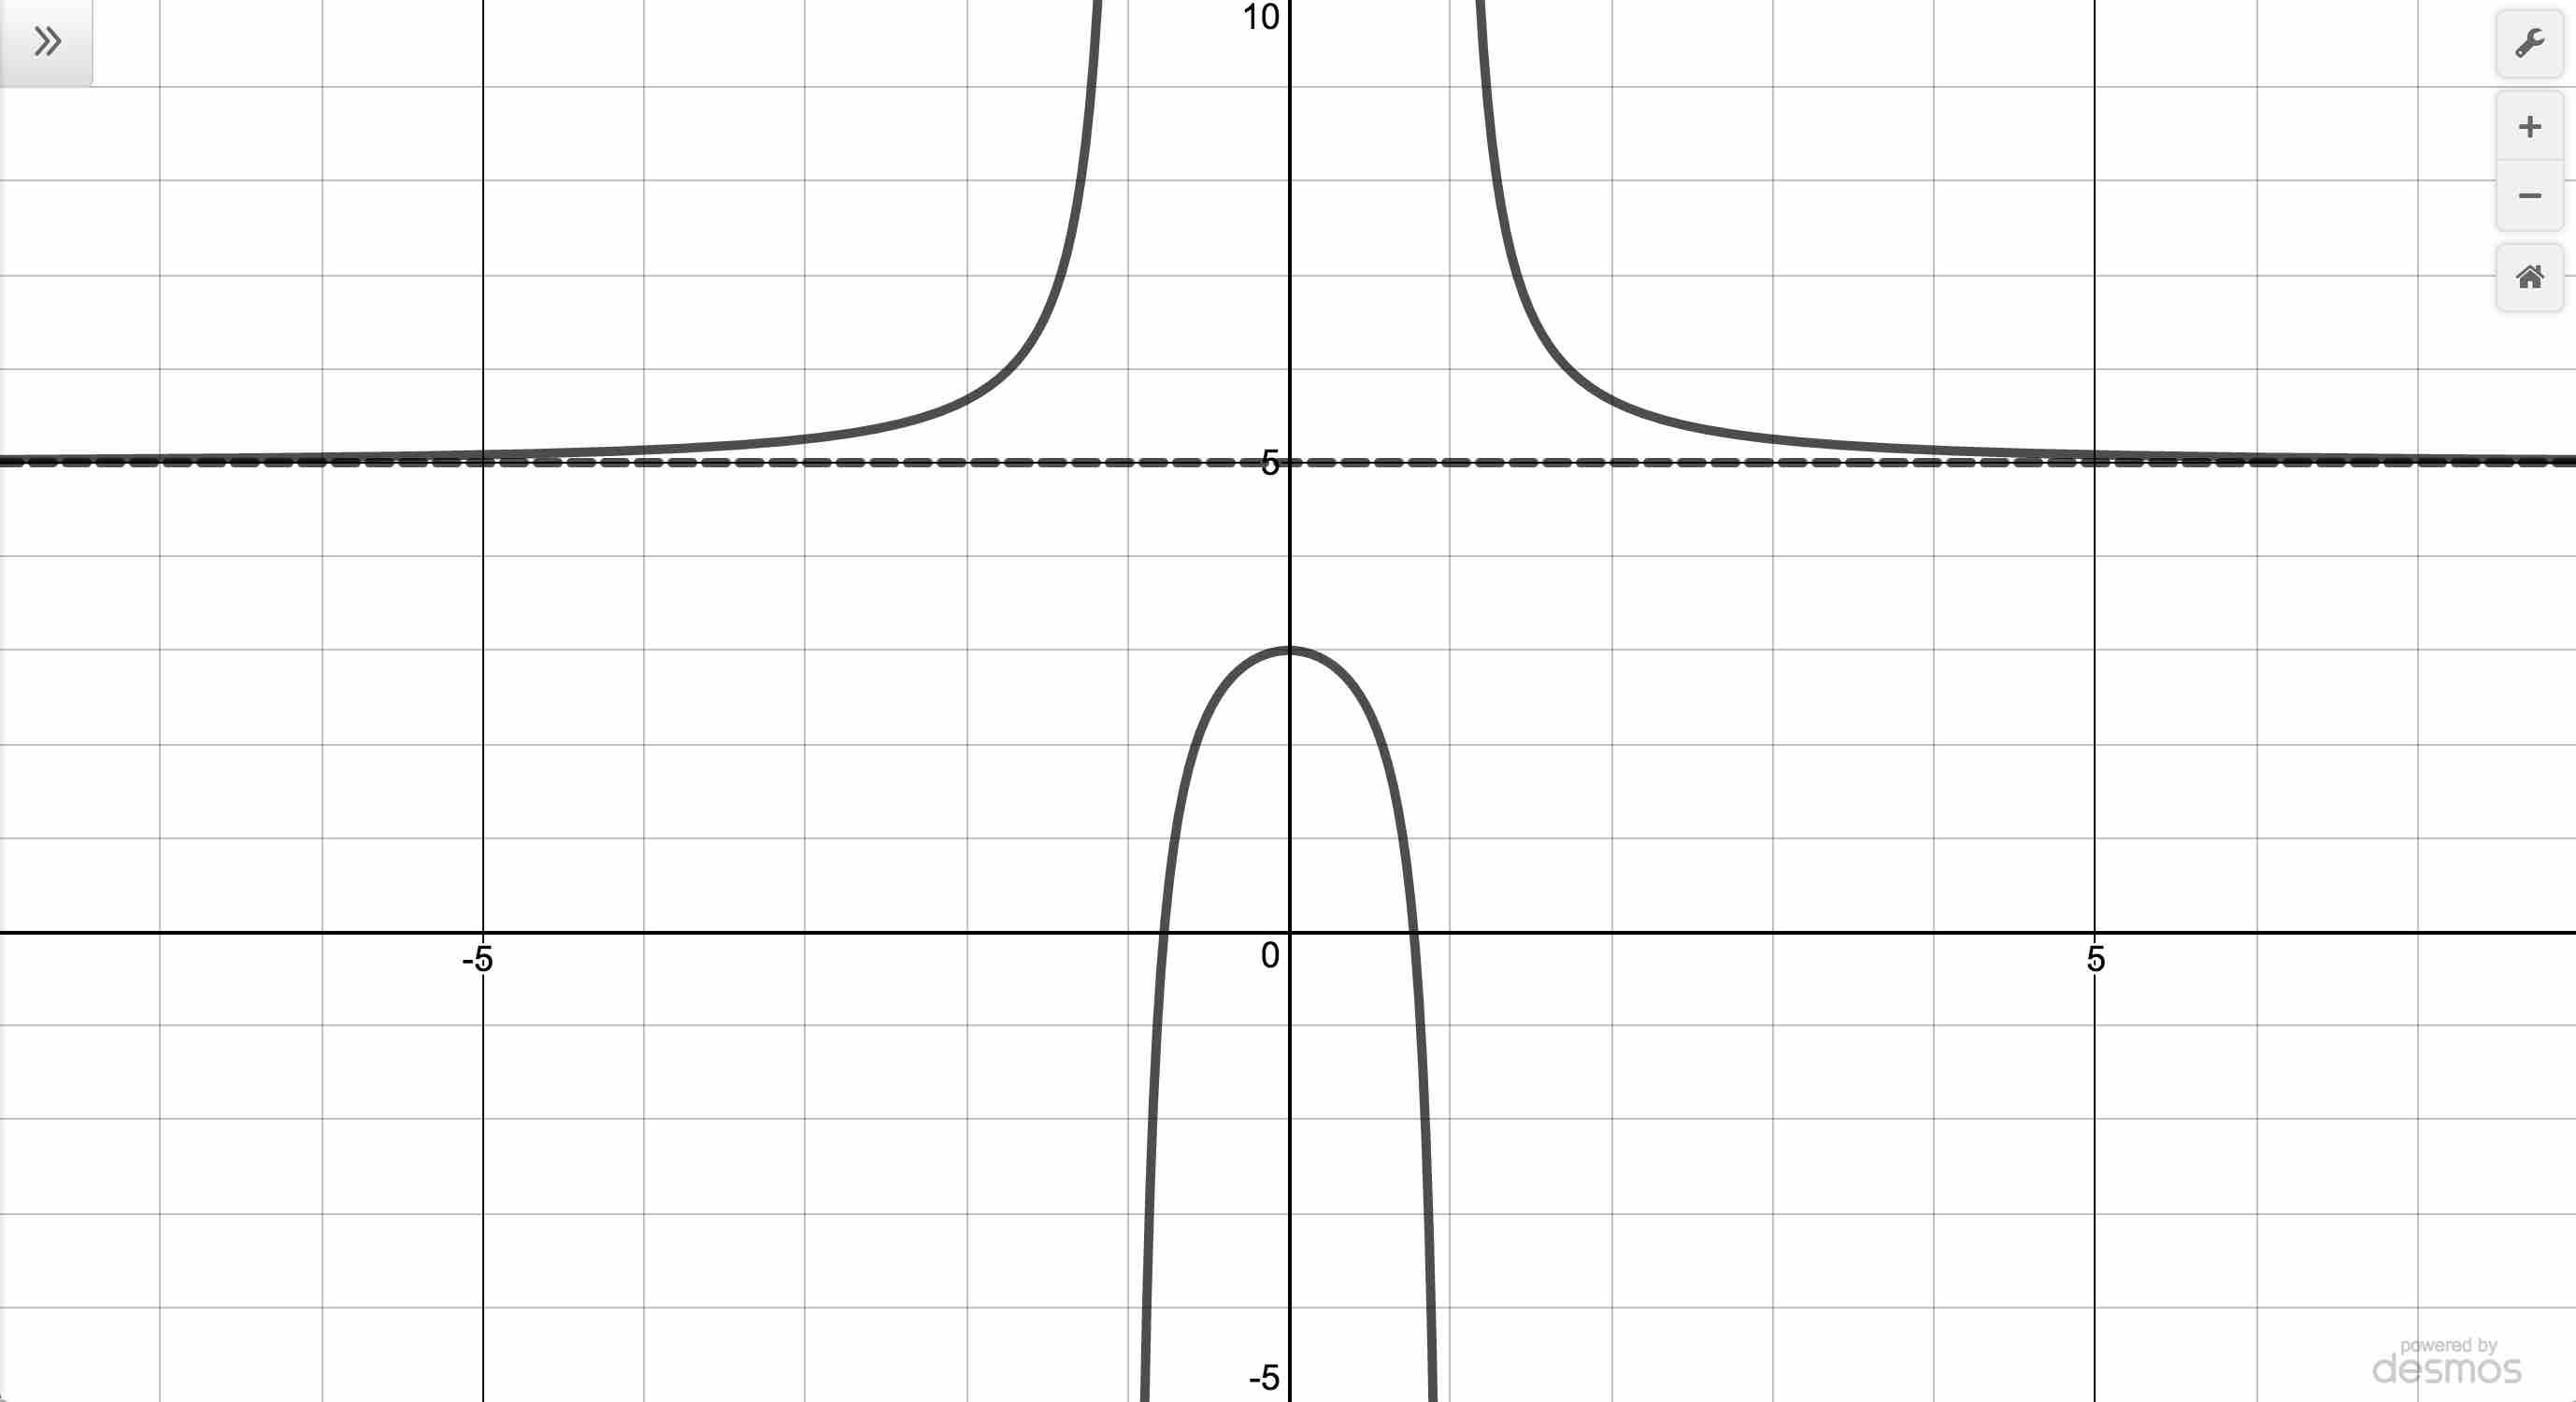
\includegraphics[width=3in]{./IntroRationalGraphics/HAEx04.jpg} \\
The graph of $y=h(t)$  & The graph of $y=r(x)$ \\


\end{tabular}
\end{center} 

\end{enumerate}

\qed

\end{ex}


We close this section with a discussion of the \textit{third} (and final!) kind of asymptote which can be associated with the graphs of rational functions. Let us return to the function $g(x) = \frac{x^2-4}{x+1}$ in Example \ref{haexample}. Performing long division,\footnote{See the remarks following Theorem \ref{hathm}.} we get $g(x) = \frac{x^2-4}{x+1} = x-1 - \frac{3}{x+1}$.  Since the term $\frac{3}{x+1} \rightarrow 0$ as $x \rightarrow \pm \infty$, it stands to reason that as $x$ becomes unbounded, the function values   $g(x) = x-1 - \frac{3}{x+1} \approx x-1$.  Geometrically, this means that the graph of $y=g(x)$ should resemble the line $y = x-1$ as $x \rightarrow \pm \infty$.  We see this play out both numerically and graphically below. (As usual, we the asymptote $y = x-1$ is denoted by a dashed line.)

\begin{center}
\begin{tabular}{cc}

$\begin{array}{|r||c|c|}  \hline

  x & g(x) & x-1 \\ \hline
 -10 & \approx -10.6667 & -11 \\  \hline
 -100 & \approx -100.9697 & -101 \\  \hline 
 -1000 &  \approx -1000.9970&   -1001 \\ \hline 
  -10000 &  \approx -10000.9997 &  -10001 \\ \hline 
  \end{array} $ & 

$\begin{array}{|r||c|c|}  \hline

  x & g(x) & x-1 \\ \hline
 10 & \approx 8.7273 &    9 \\\hline
 100 & \approx 98.9703 &   99 \\ \hline 
 1000 &  \approx 998.9970 &  999 \\ \hline 
  10000 &  \approx 9998.9997 &   9999 \\ \hline 
  \end{array} $ \\
  
  \end{tabular}
  \end{center}
  
  
\begin{center}
   
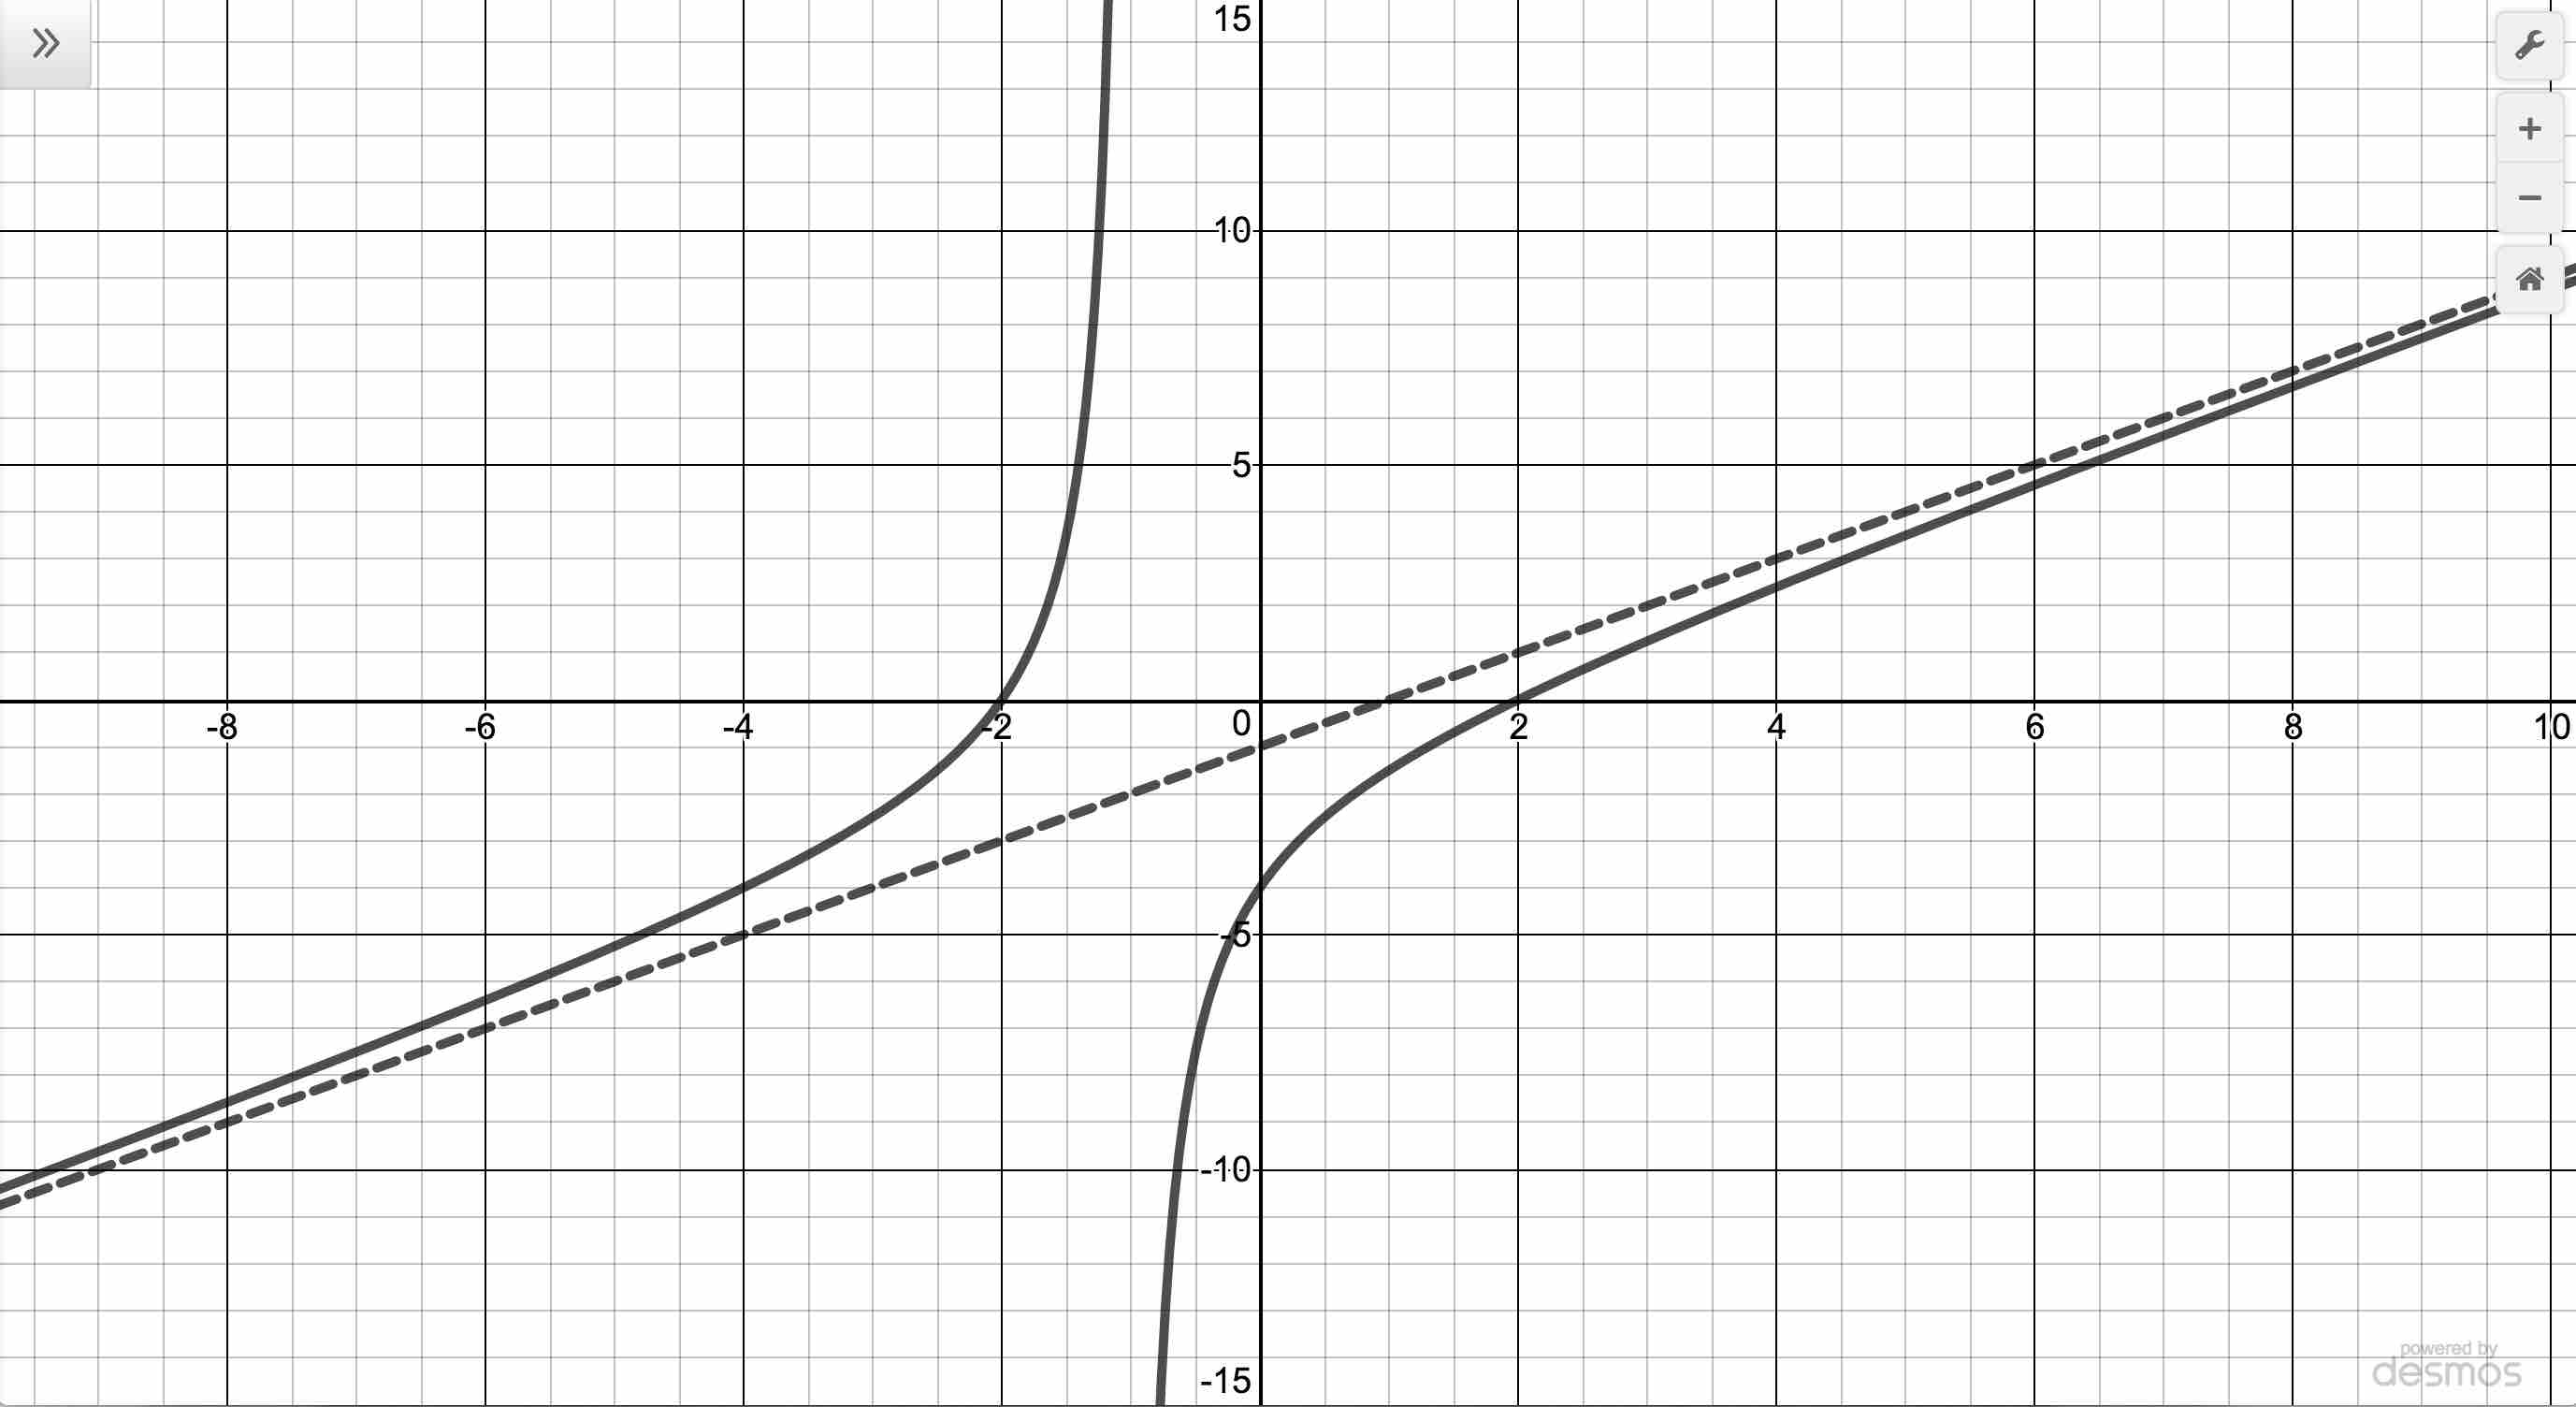
\includegraphics[width=4in]{./IntroRationalGraphics/SAEx01.jpg}

\end{center}
 
The way we symbolize the relationship between the end behavior of $y=g(x)$ with that of the line $y=x-1$ is to write `as $x \rightarrow \pm \infty$, $g(x) \rightarrow x-1$' in order to have some notational consistency with what we have done earlier in this section when it comes to end behavior.\footnote{Other notations include $g(x) \asymp x-1$ or $g(x) \sim x-1$.}  In this case, we say the line $y=x-1$ is a \index{asymptote ! slant (oblique)} \index{slant asymptote} \index{oblique asymptote} \textbf{slant asymptote}\footnote{Also called an `oblique' asymptote in some, ostensibly higher class (and more expensive), texts.}  to the graph of $y=g(x)$.  Informally, the graph of a rational function has a slant asymptote if, as $x \rightarrow \infty$ or as $x \rightarrow -\infty$, the graph resembles a non-horizontal, or `slanted' line.  Formally, we define a slant asymptote as follows.


\medskip


\colorbox{ResultColor}{\bbm

\begin{defn} \label{sa} The line $y = mx+b$ where $m \neq 0$  is called a \index{asymptote ! slant ! formal definition of}\index{slant asymptote ! formal definition of}\textbf{slant asymptote} of the graph of a function $y=f(x)$ if as $x \rightarrow -\infty$ or as $x \rightarrow \infty$, $f(x)  \rightarrow mx+b$.


\end{defn}
\ebm}

\medskip


A few remarks are in order.  First, note that the stipulation $m \neq 0$ in Definition \ref{sa} is what makes the `slant' asymptote `slanted' as opposed to the case when $m=0$ in which case we'd have a horizontal asymptote.  Secondly, while we have motivated what me mean intuitively by the notation `$f(x)  \rightarrow mx+b$,' like so many ideas in this section, the formal definition requires Calculus.  Another way to express this sentiment, however, is to rephrase `$f(x)  \rightarrow mx+b$' as `$[f(x) - (mx+b)] \rightarrow 0$.'  In other words, the graph of $y=f(x)$ has the \textit{slant} asymptote $y = mx+b$ if and only if the graph of $y = f(x) - (mx+b)$ has a \textit{horizontal} asymptote $y=0$.  If we wanted to, we could introduce the notations $f(x) \rightarrow (mx+b)^{+}$ to mean $[f(x)-(mx+b)] \rightarrow 0^{+}$ and $f(x) \rightarrow (mx+b)^{-}$ to mean $[f(x)-(mx+b)] \rightarrow 0^{-}$, but these non-standard notations.\footnote{With the introduction of the symbol `\textinterrobang' in the next section, the authors feel we are in enough trouble already.}



Our next task is to determine the conditions under which the graph of a rational function has a slant asymptote, and if it does, how to find it.  In the case of $g(x) = \frac{x^2-4}{x+1}$, the degree of the numerator $x^2-4$ is $2$, which is \textit{exactly one more} than the degree if its denominator $x+1$ which is $1$.  This results in a \textit{linear} quotient polynomial, and it is this quotient polynomial which is the slant asymptote.  Generalizing this situation gives us the following theorem.\footnote{Once again, this theorem is brought to you courtesy of Theorem \ref{polydiv} and Calculus.}

\medskip

\colorbox{ResultColor}{\bbm

\begin{thm} \textbf{Determination of Slant Asymptotes:} \label{sathm} Suppose $r$ is a rational function and $r(x) = \frac{p(x)}{q(x)}$, where the degree of $p$ is \textit{exactly} one more than the degree of $q$.  Then the graph of $y=r(x)$ has \index{asymptote ! slant ! determination of}\index{slant asymptote ! determination of} the slant asymptote $y=L(x)$ where $L(x)$ is the quotient obtained by dividing $p(x)$ by $q(x)$.

\end{thm}
\ebm}

\medskip

In the same way that Theorem \ref{hathm} gives us an easy way to see if the graph of a rational function $r(x) = \frac{p(x)}{q(x)}$ has a horizontal asymptote by comparing the degrees of the numerator and denominator, Theorem \ref{sathm} gives us an easy way to check for slant asymptotes.  Unlike Theorem \ref{hathm}, which gives us a quick way to \textit{find} the horizontal asymptotes (if any exist), Theorem \ref{sathm} gives us no such `short-cut'.  If a slant asymptote exists, we have no recourse but to use long division to find it.\footnote{That's OK, though.  In the next section, we'll use long division to analyze end behavior and it's worth the effort!}  

\begin{ex} \label{saexample}  For each of the following functions:

\begin{itemize}

\item find the slant asymptote, if it exists.

\item  verify your answer using a graphing utility.

\item  investigate any apparent symmetry of the graph about the $y$-axis or origin.

\end{itemize}


\begin{multicols}{2}
\begin{enumerate}

\item  $f(x) = \dfrac{x^2-4x+2}{1-x}$  

\item  \label{sacancel} $g(t) = \dfrac{t^2-4}{t-2}$

\setcounter{HW}{\value{enumi}}
\end{enumerate}
\end{multicols}

\begin{multicols}{2}
\begin{enumerate}
\setcounter{enumi}{\value{HW}}


\item  $h(x) = \dfrac{x^3+1}{x^2-4}$

\item  $r(t) = 2t-1+\dfrac{4t^3}{1-t^2}$ \vphantom{$h(x) = \dfrac{x^3+1}{x^2-4}$}

\setcounter{HW}{\value{enumi}}
\end{enumerate}
\end{multicols}



{\bf Solution.}

\begin{enumerate}

\item  The degree of the numerator is $2$ and the degree of the denominator is $1$, so Theorem \ref{sathm} guarantees us a slant asymptote.  To find it, we divide $1-x = -x+1$ into $x^2-4x+2$ and get a quotient of $-x+3$, so our slant asymptote is $y=-x+3$.  We confirm this graphically below.

\item  As with the previous example, the degree of the numerator $g(t) = \frac{t^2-4}{t-2}$ is $2$ and the degree of the denominator is $1$, so Theorem \ref{sathm} applies.  In this case, 

\[ g(t) = \frac{t^2-4}{t-2} = \frac{(t+2)(t-2)}{(t-2)} = \frac{(t+2) \cancel{(t-2)}}{\cancelto{1}{(t-2)}} = t+2, \quad t \neq 2\]

so we have that the slant asymptote $y=t+2$ is identical to the graph of $y=g(t)$ except at $t=2$ (where the latter has a `hole' at $(2,4)$.) While the word `asymptote' has the connotation of `approaching but not equaling,' Definitions \ref{sa} and  \ref{ha} allow for these extreme cases.

\begin{center}
\begin{tabular}{cc}

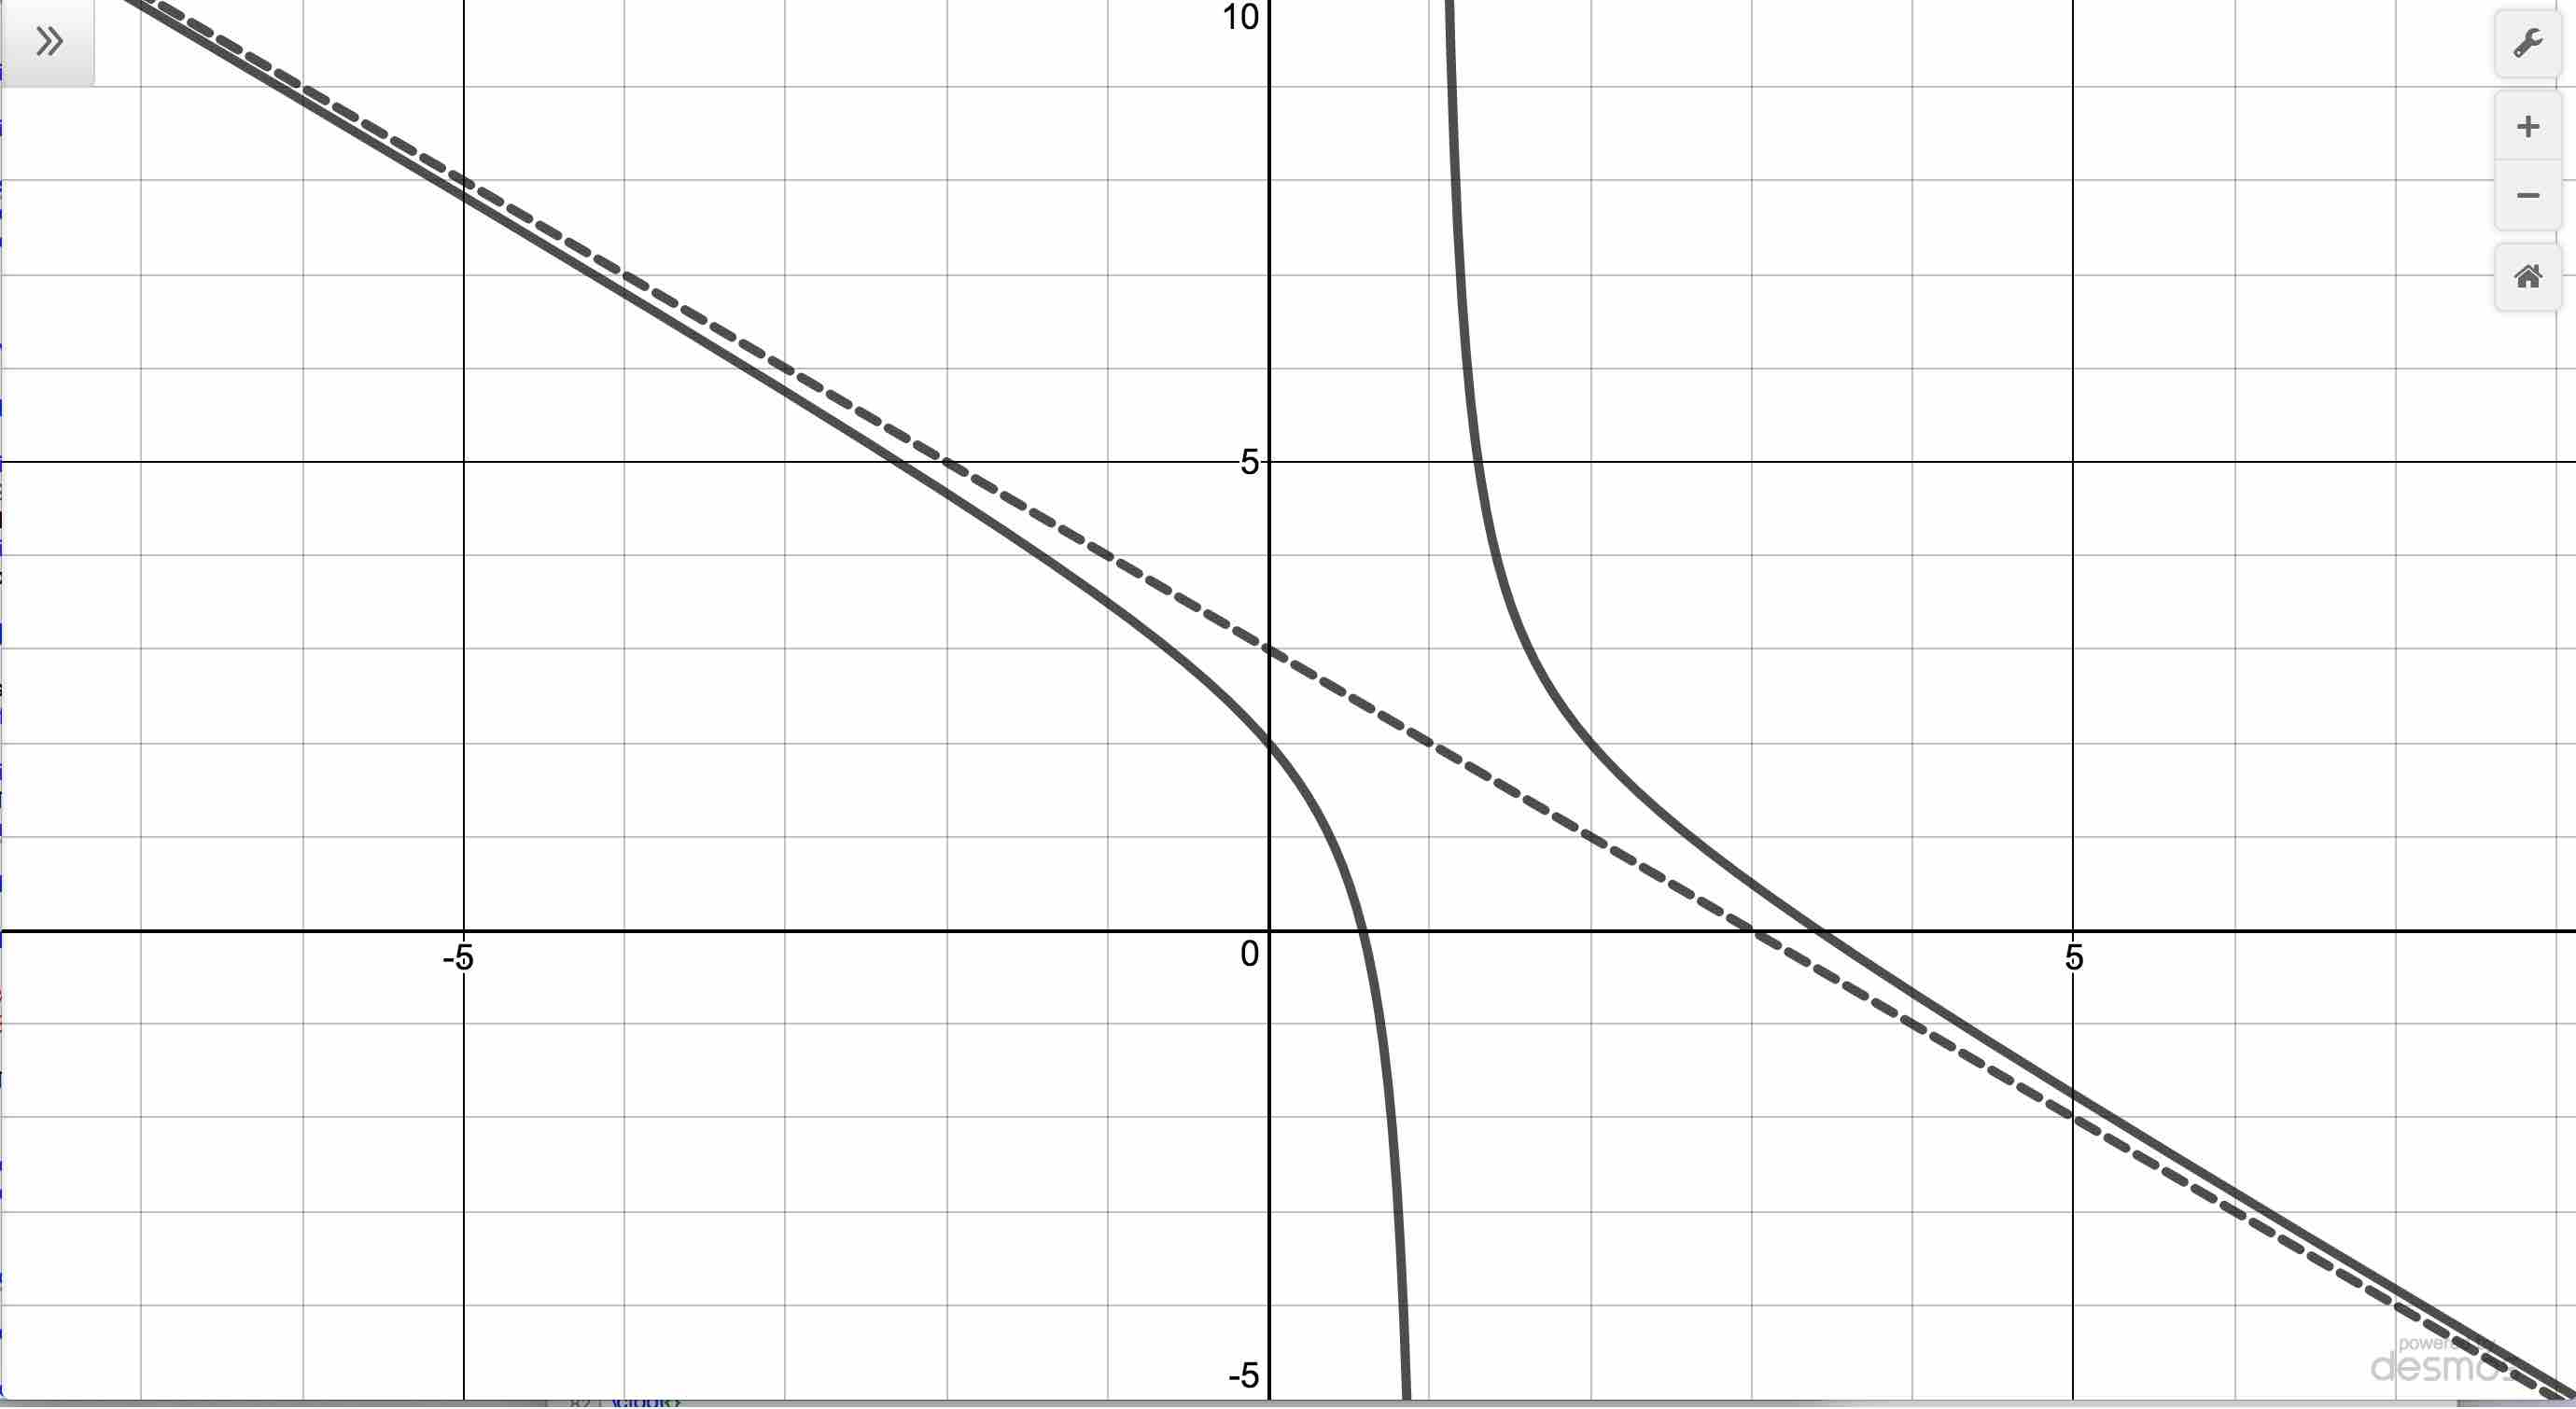
\includegraphics[width=3in]{./IntroRationalGraphics/SAEx02.jpg}  & 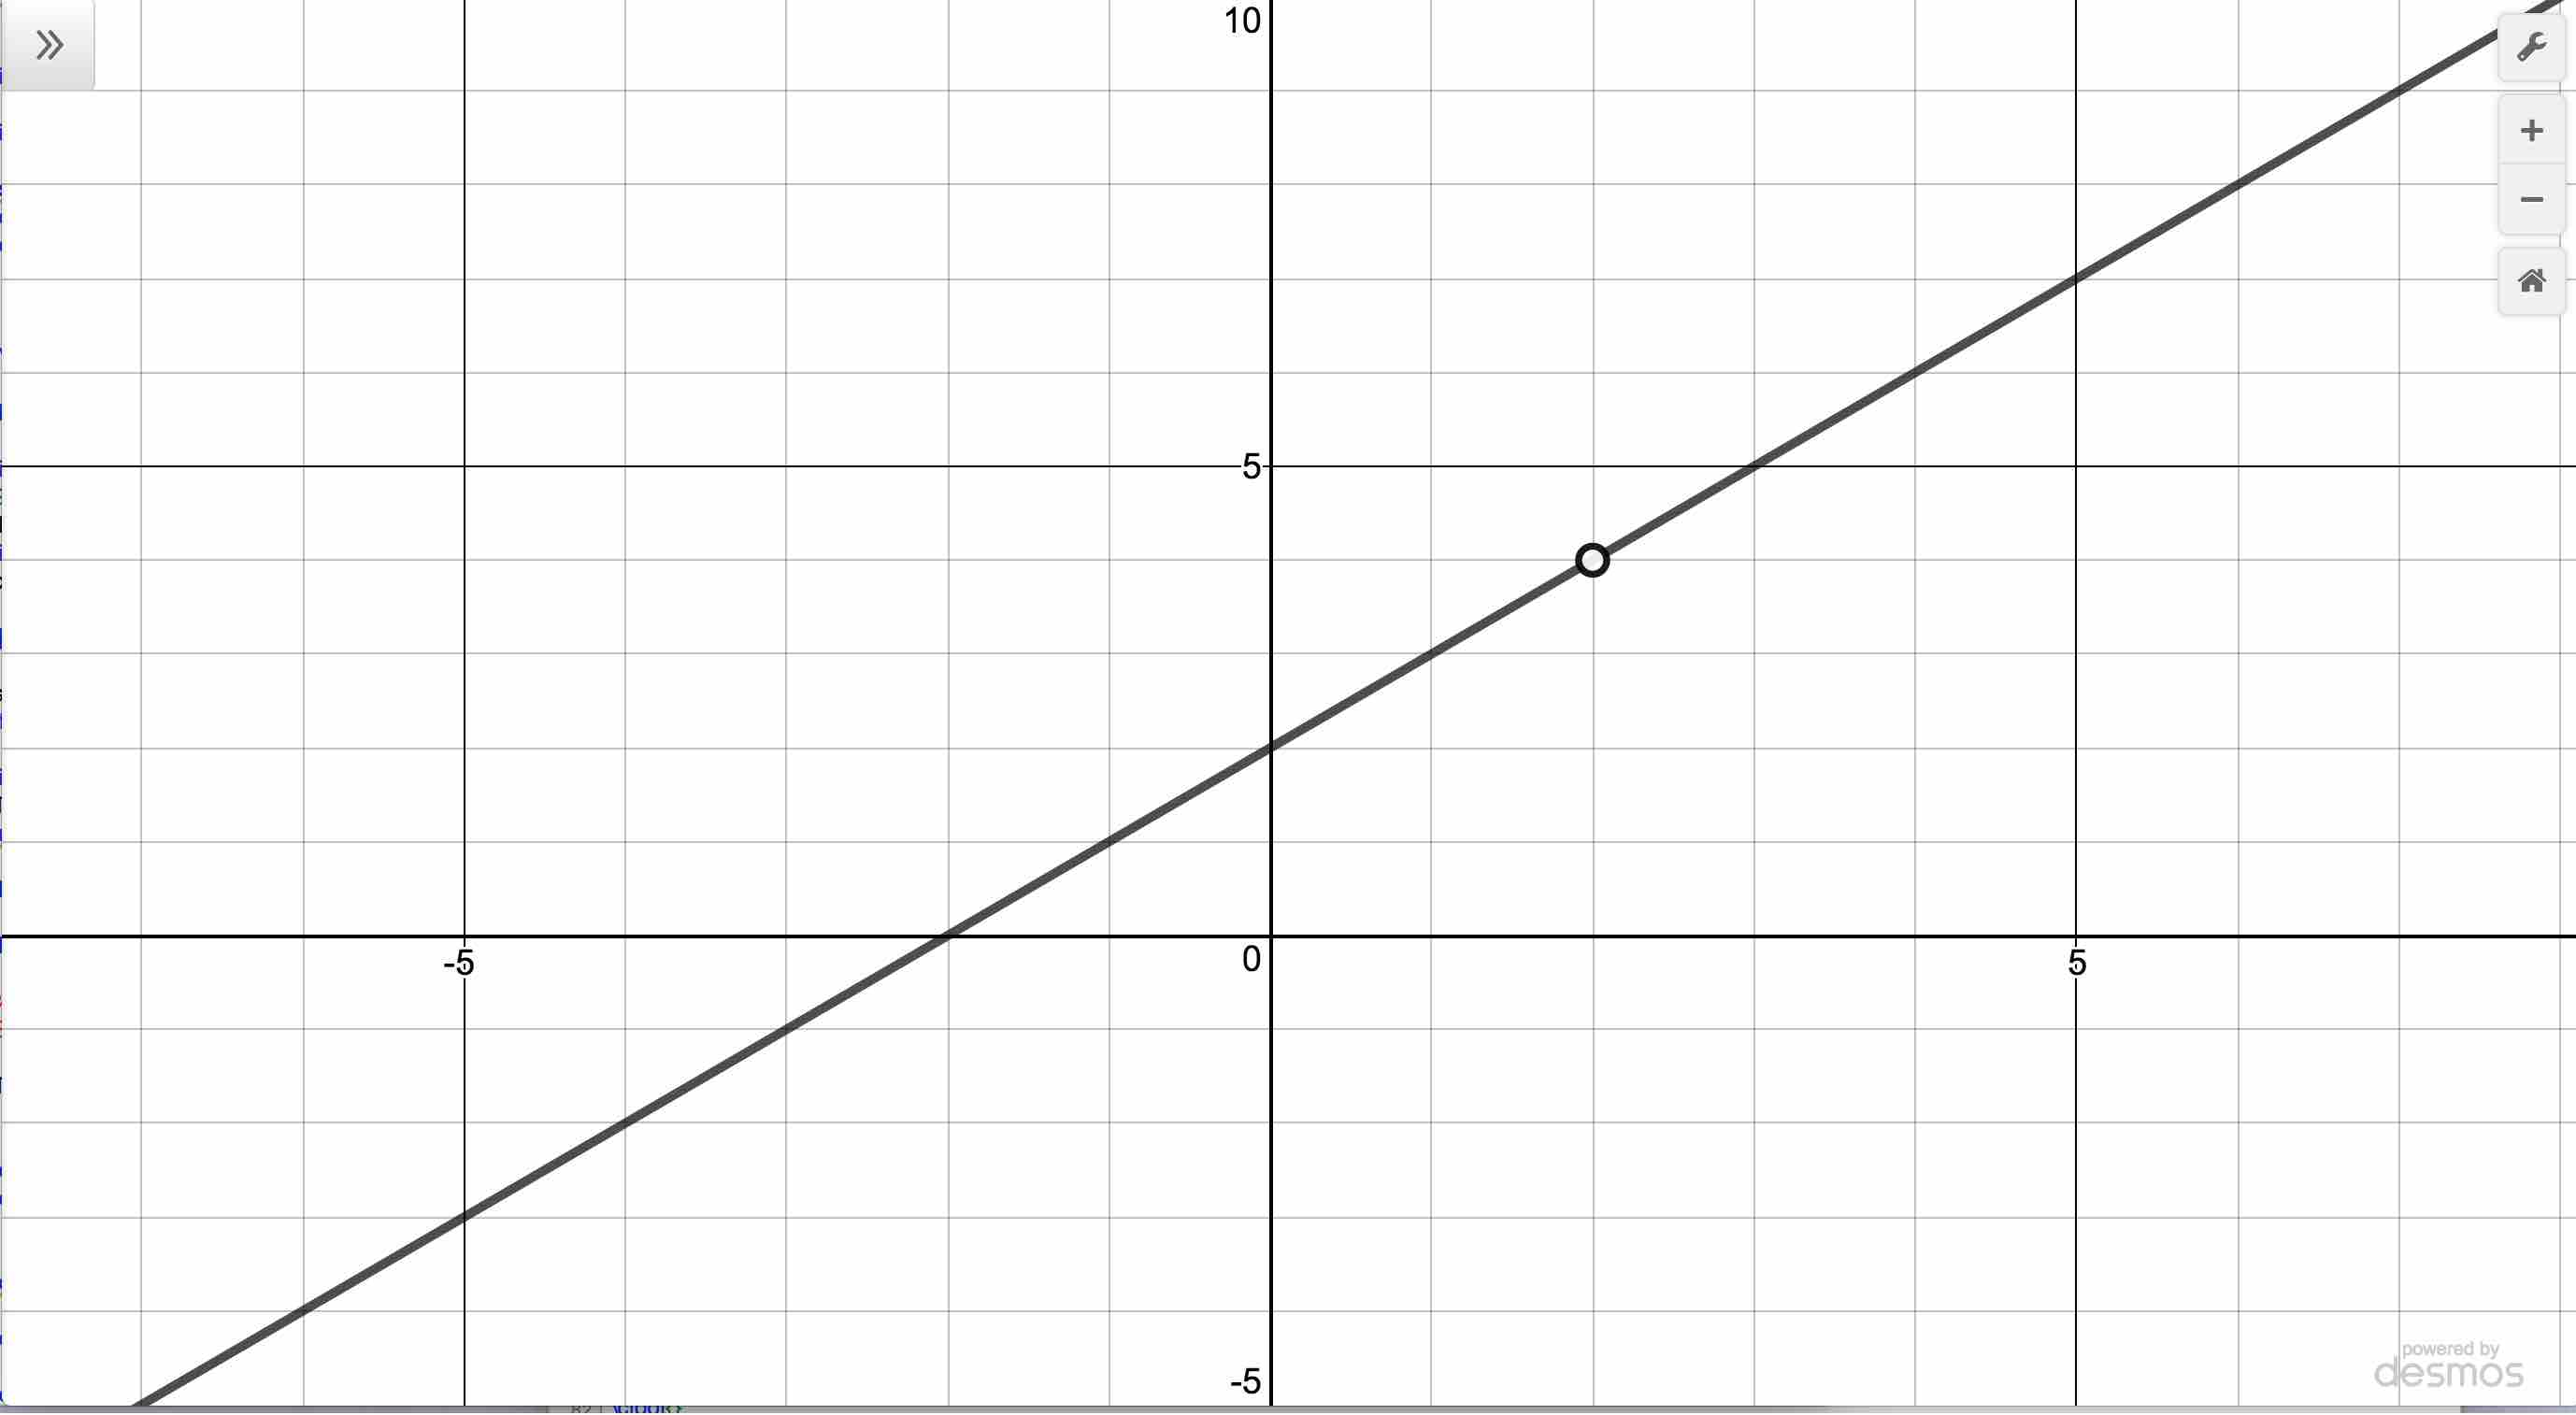
\includegraphics[width=3in]{./IntroRationalGraphics/SAEx03.jpg} \\
The graph of $y=f(x)$  & The graph of $y=g(t)$ \\


\end{tabular}
\end{center} 

\item   For $h(x) = \frac{x^3+1}{x^2-4}$, the degree of the numerator is $3$ and the degree of the denominator is $2$ so again, we are guaranteed the existence of a slant asymptote.  The long division $\left(x^3+1 \right) \div \left(x^2-4\right)$ gives a quotient of just $x$, so our slant asymptote is the line $y=x$.  The graphing utility confirms this.  Note the graph of $h$ appears to be symmetric about the origin.  We check $h(-x) = \frac{(-x)^3+1}{(-x)^2-4} = \frac{-x^3+1}{x^2-4} = - \frac{x^3-1}{x^2-4}$.  However, $-h(x) = - \frac{x^3+1}{x^2-4}$, so it appears as if $h(-x) \neq -h(x)$ for all $x$.  Checking $x=1$, we find $h(1) = -\frac{2}{3}$ but $h(-1) = 0$ which shows the graph of $h$, is in fact,  \textit{not} symmetric about the origin.

\item  For our last example,  $r(t) = 2t-1+\frac{4t^3}{1-t^2}$, the expression $r(t)$ is not in the form to apply Theorem \ref{sathm} directly.  We can, nevertheless, appeal to the spirit of the theorem and use long division to rewrite the term $\frac{4t^3}{1-t^2} = -4t + \frac{4t}{1-t^2}$.  We then get:

 \[ \begin{array}{rcl}
 
 r(t) & = & 2t-1+\dfrac{4t^3}{1-t^2} \\
       &= &  2t-1-4t+\dfrac{4t}{1-t^2} \\
       & = & -2t-1 + \dfrac{4t}{1-t^2} \\ \end{array}\]
       
As $t \rightarrow \pm \infty$,  Theorem \ref{EBPolynomials} gives  $\frac{4t}{1-t^2} \approx \frac{4t}{-t^2} = -\frac{4}{t} \rightarrow 0$.  Hence, as $t \rightarrow \pm \infty$, $r(t) \rightarrow -2t-1$, so $y = -2t-1$ is the slant asymptote to the graph as confirmed by the graphing utility below.  from a distance, the graph of $r$ appears to be symmetric about the origin.  However, if we look carefully, we see the $y$-intercept is $(0,-1)$, as borne out by the computation $r(0) = -1$.  Hence $r$ cannot be odd.  (Do you see why?)

\begin{center}
\begin{tabular}{cc}

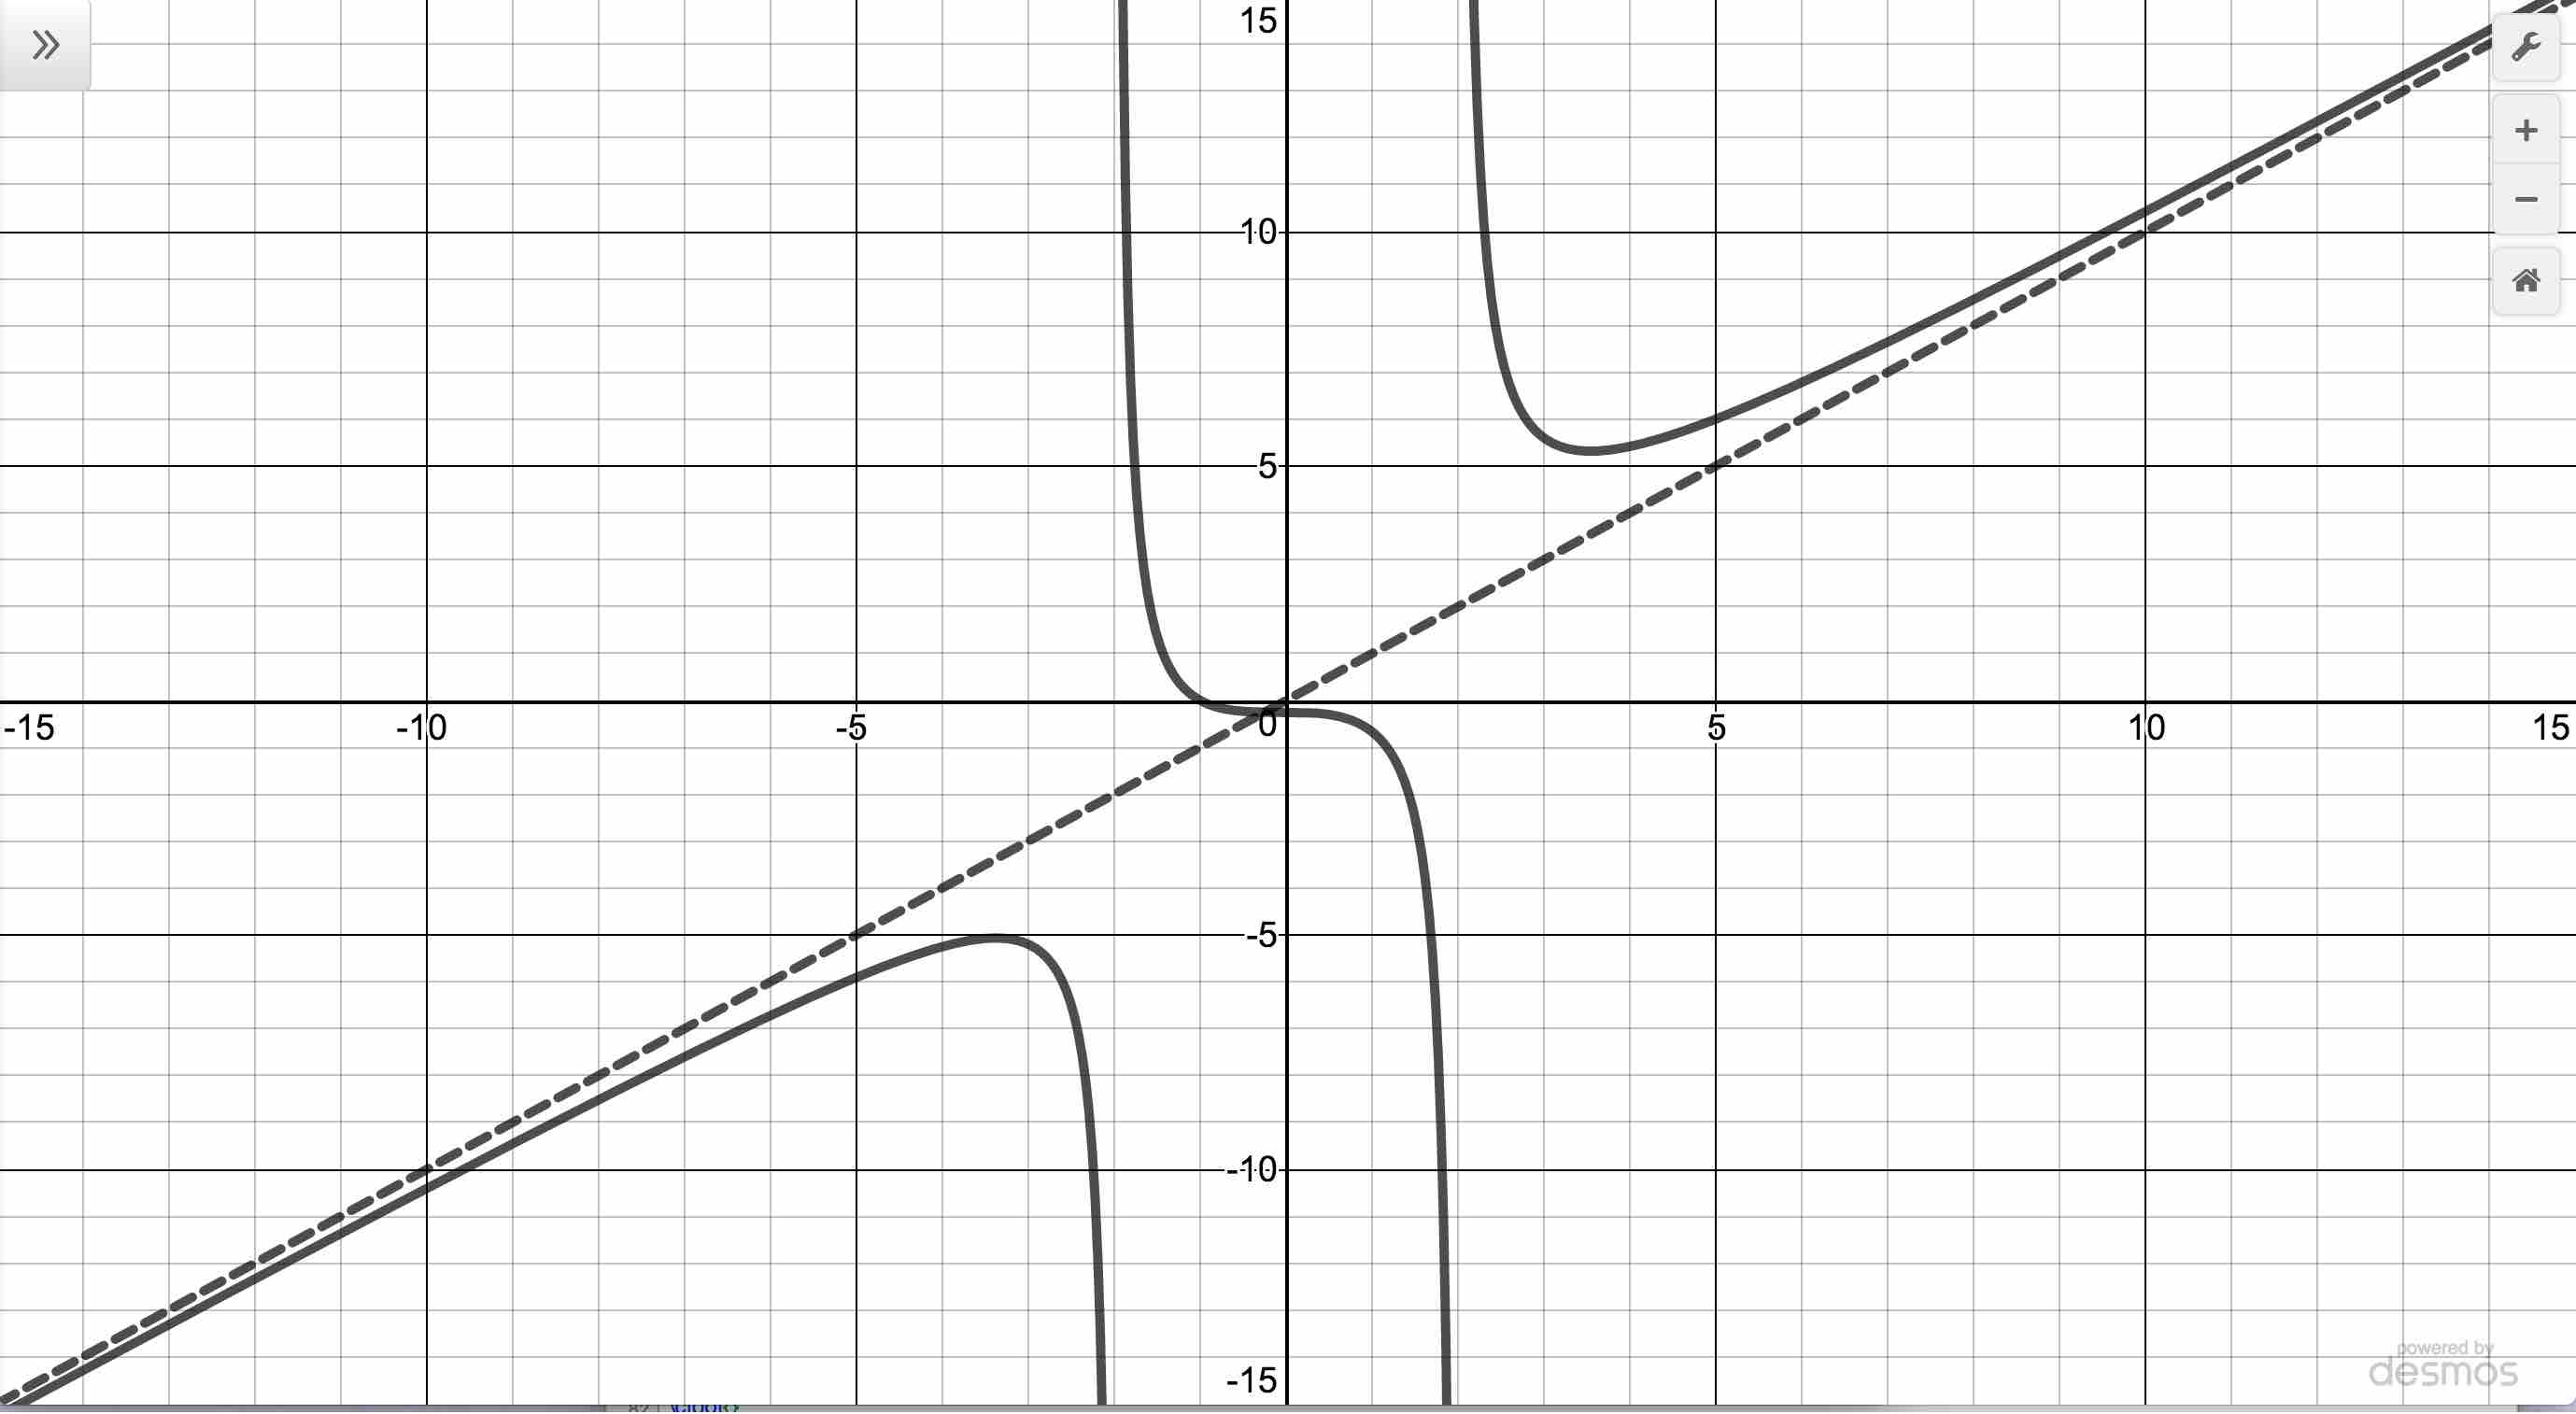
\includegraphics[width=3in]{./IntroRationalGraphics/SAEx04.jpg}  & 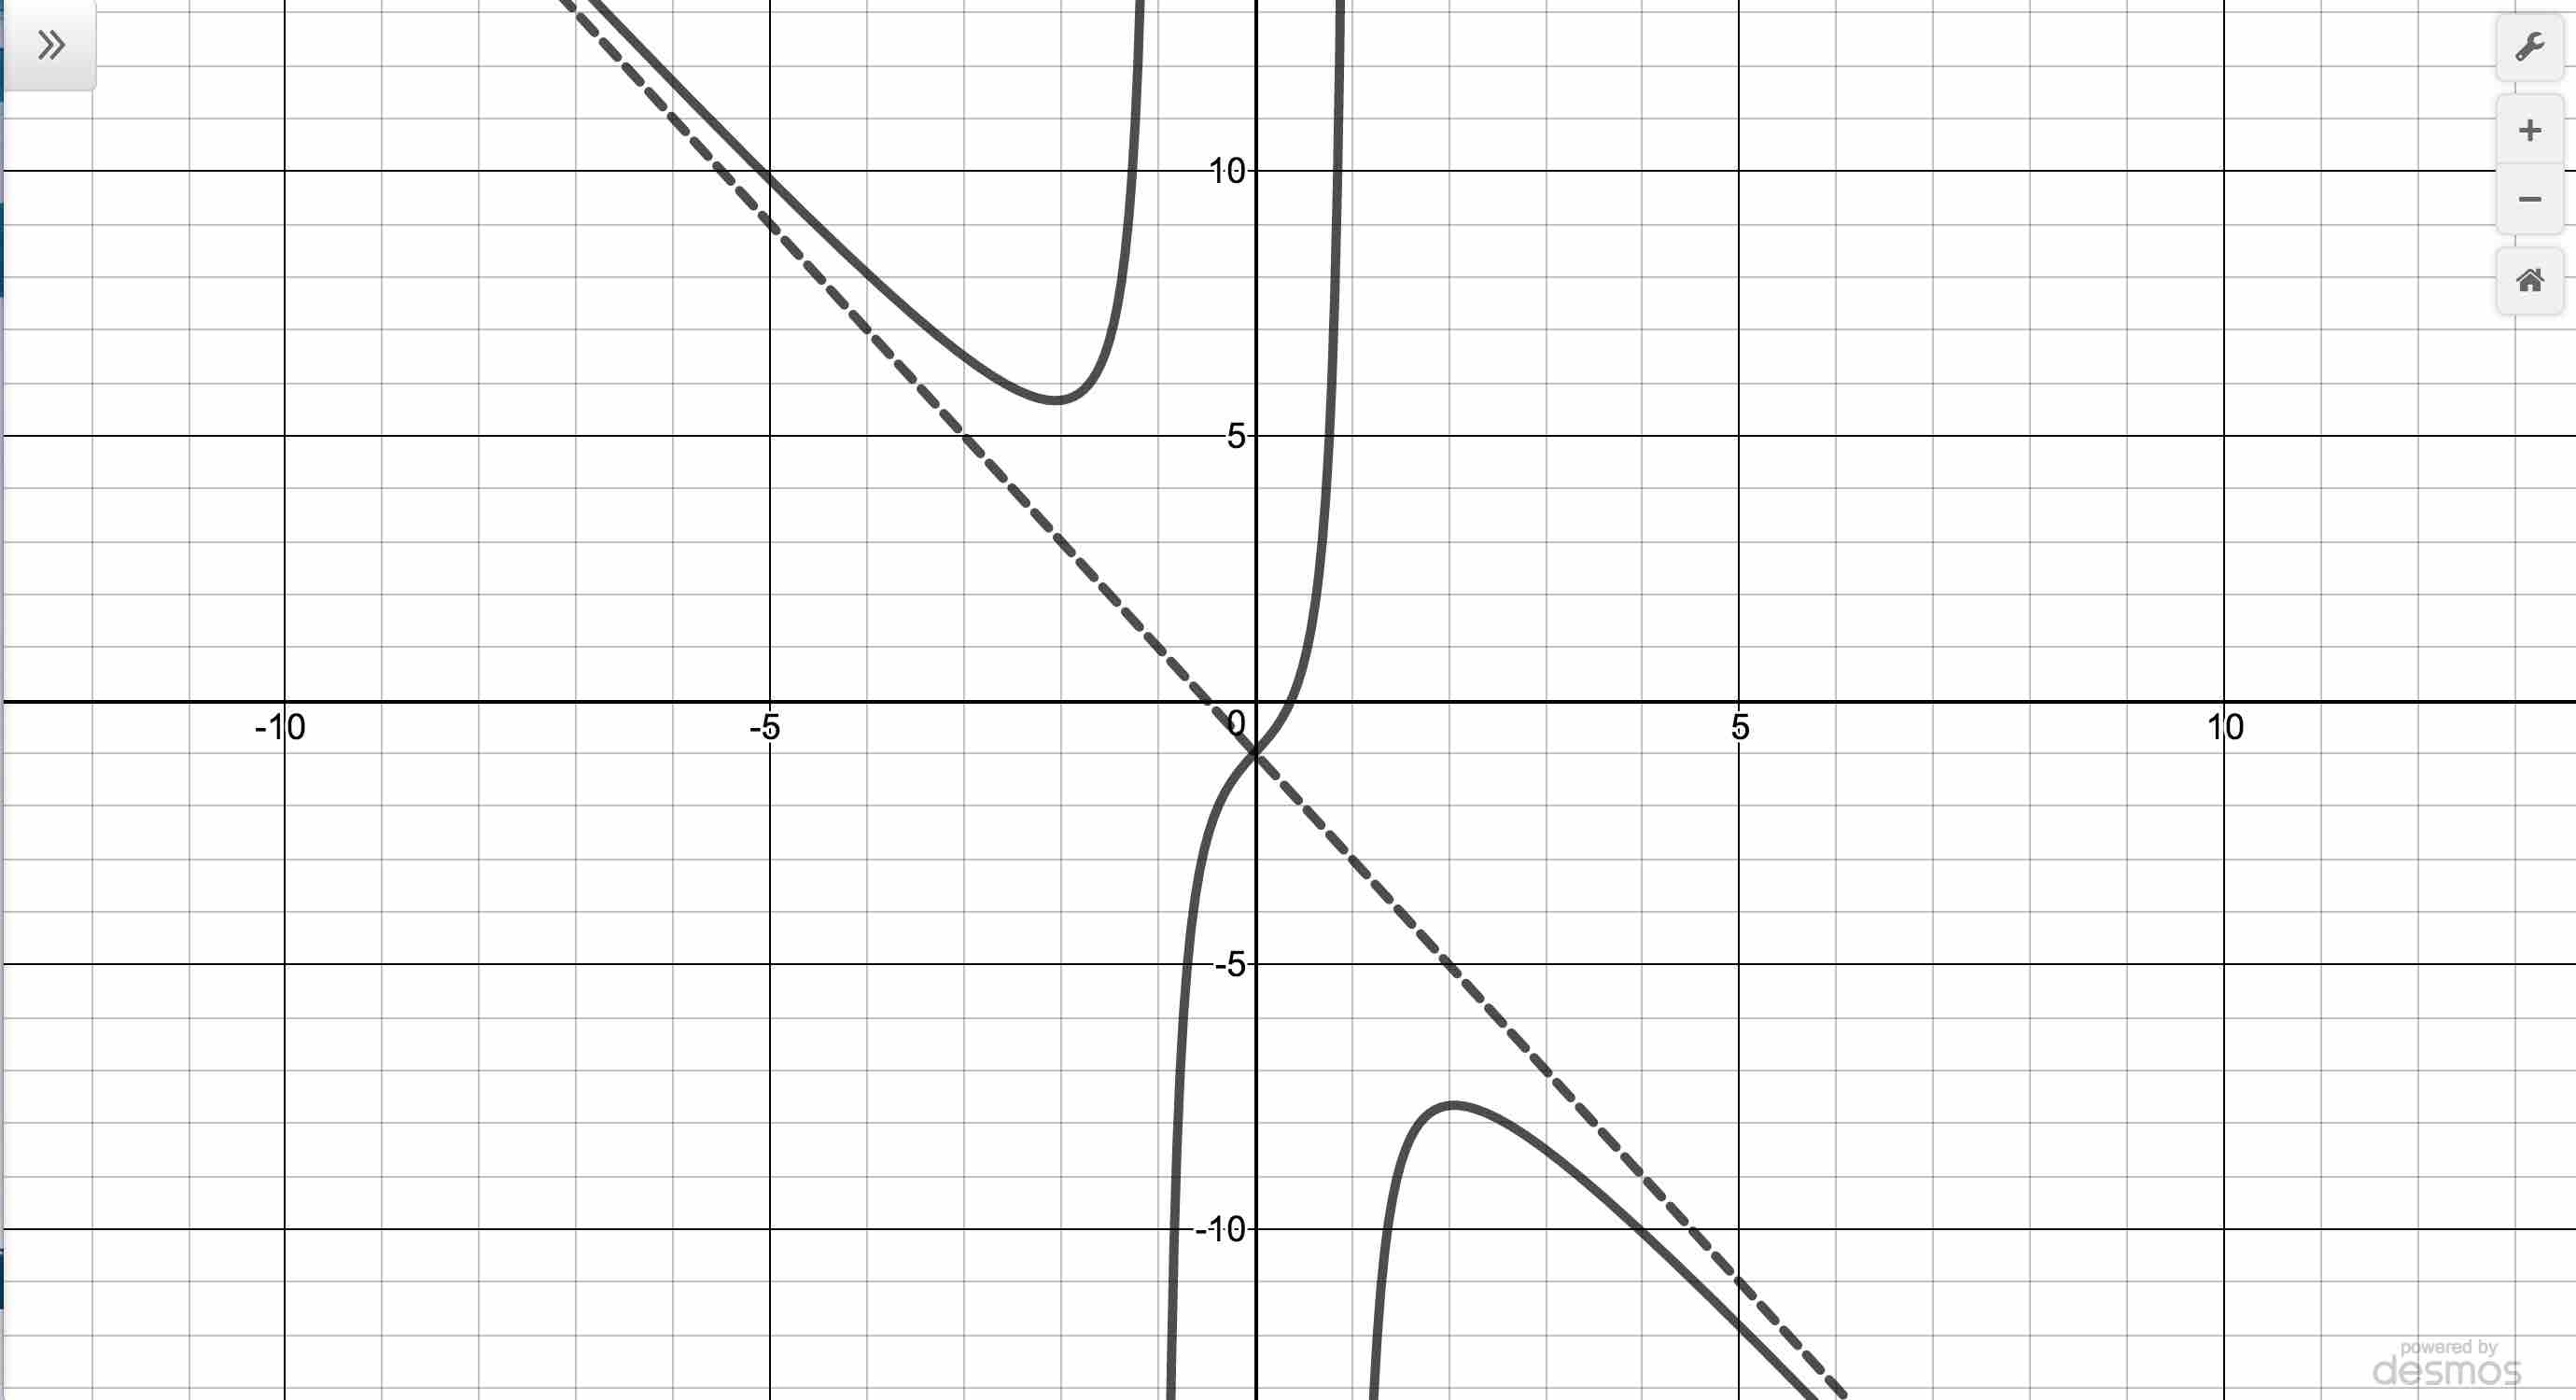
\includegraphics[width=3in]{./IntroRationalGraphics/SAEx05.jpg} \\
The graph of $y=h(x)$  & The graph of $y=r(t)$ \\


\end{tabular}
\end{center}

\qed

\end{enumerate}

\end{ex}

Our last example gives a real-world application of a slant asymptote. The problem features the concept of \textbf{average profit}. The average profit, denoted $\overline{P}(x)$,  is the total profit, $P(x)$,  divided by the number of items sold, $x$. In English, the average profit tells us the profit made per item sold. It, along with average cost, is defined below.

\colorbox{ResultColor}{\bbm

\begin{defn} \label{averagecostprofit} Let $C(x)$ and $P(x)$ represent the cost and profit to make and sell $x$ items, respectively.

\begin{itemize}

\item    The \index{average cost}\index{cost ! average} \textbf{average cost}, $\overline{C}(x) = \dfrac{C(x)}{x}$, $x > 0$.  

\textbf{NOTE:}  The average cost is the cost per item produced.

\item   The \index{average profit}\index{profit ! average} \textbf{average profit}, $\overline{P}(x) = \dfrac{P(x)}{x}$, $x > 0$.  

\textbf{NOTE:}  The average profit is the profit  per item sold.

\end{itemize}

\end{defn}

\ebm}

You'll explore average cost (and its relation to variable cost) in Exercise \ref{averagevariablecostexercise}.  For now, we refer the reader to to Example \ref{PortaBoyProfit}  in Section \ref{QuadraticFunctions}.

\begin{ex} \label{PortaBoyAverageProfit}  Recall the profit (in dollars) when $x$ PortaBoy game systems are produced and sold is given by $P(x) =  -1.5x^2+170x-150$, $0 \leq x \leq 166$.

\begin{enumerate}

\item  Find and simplify an expression for the average profit, $\overline{P}(x)$.  What is the domain of $\overline{P}$?

\item Find and interpret $\overline{P}(50)$.

\item Determine the slant asymptote to the graph of $y = \overline{P}(x)$.  Check your answer using a graphing utility.

\item  Interpret the slope of the slant asymptote.


\end{enumerate}

{\bf Solution.}

\begin{enumerate}

\item  We find $\overline{P}(x)  = \frac{P(x)}{x} = \frac{ -1.5x^2+170x-150}{x} = -1.5x + 170 + \frac{150}{x}$.  Since the domain of $P$ is $[0, 166]$ but $x \neq 0$, the domain of $\overline{P}$ is $(0, 166]$.

\item  We find $\overline{P}(50) = -1.5(50)+170 + \frac{150}{50} = 98$.  This means that when $50$ PortaBoy systems are sold, the average profit is $\$ 98$ per system.

\item  Technically, the graph of $y = \overline{P}(x)$ has no slant asymptote since the domain of the function is restricted to $(0, 166]$.  That being said, if we were to let $x \rightarrow \infty$, the term $\frac{150}{x} \rightarrow 0$, so we'd  have $\overline{P}(x)  \rightarrow -1.5x + 170$.  This means the slant asymptote would be $y = -1.5x + 170$.  We graph $y = \overline{P}(x)$ and $y = -1.5x+170$.

  
\begin{center}
   
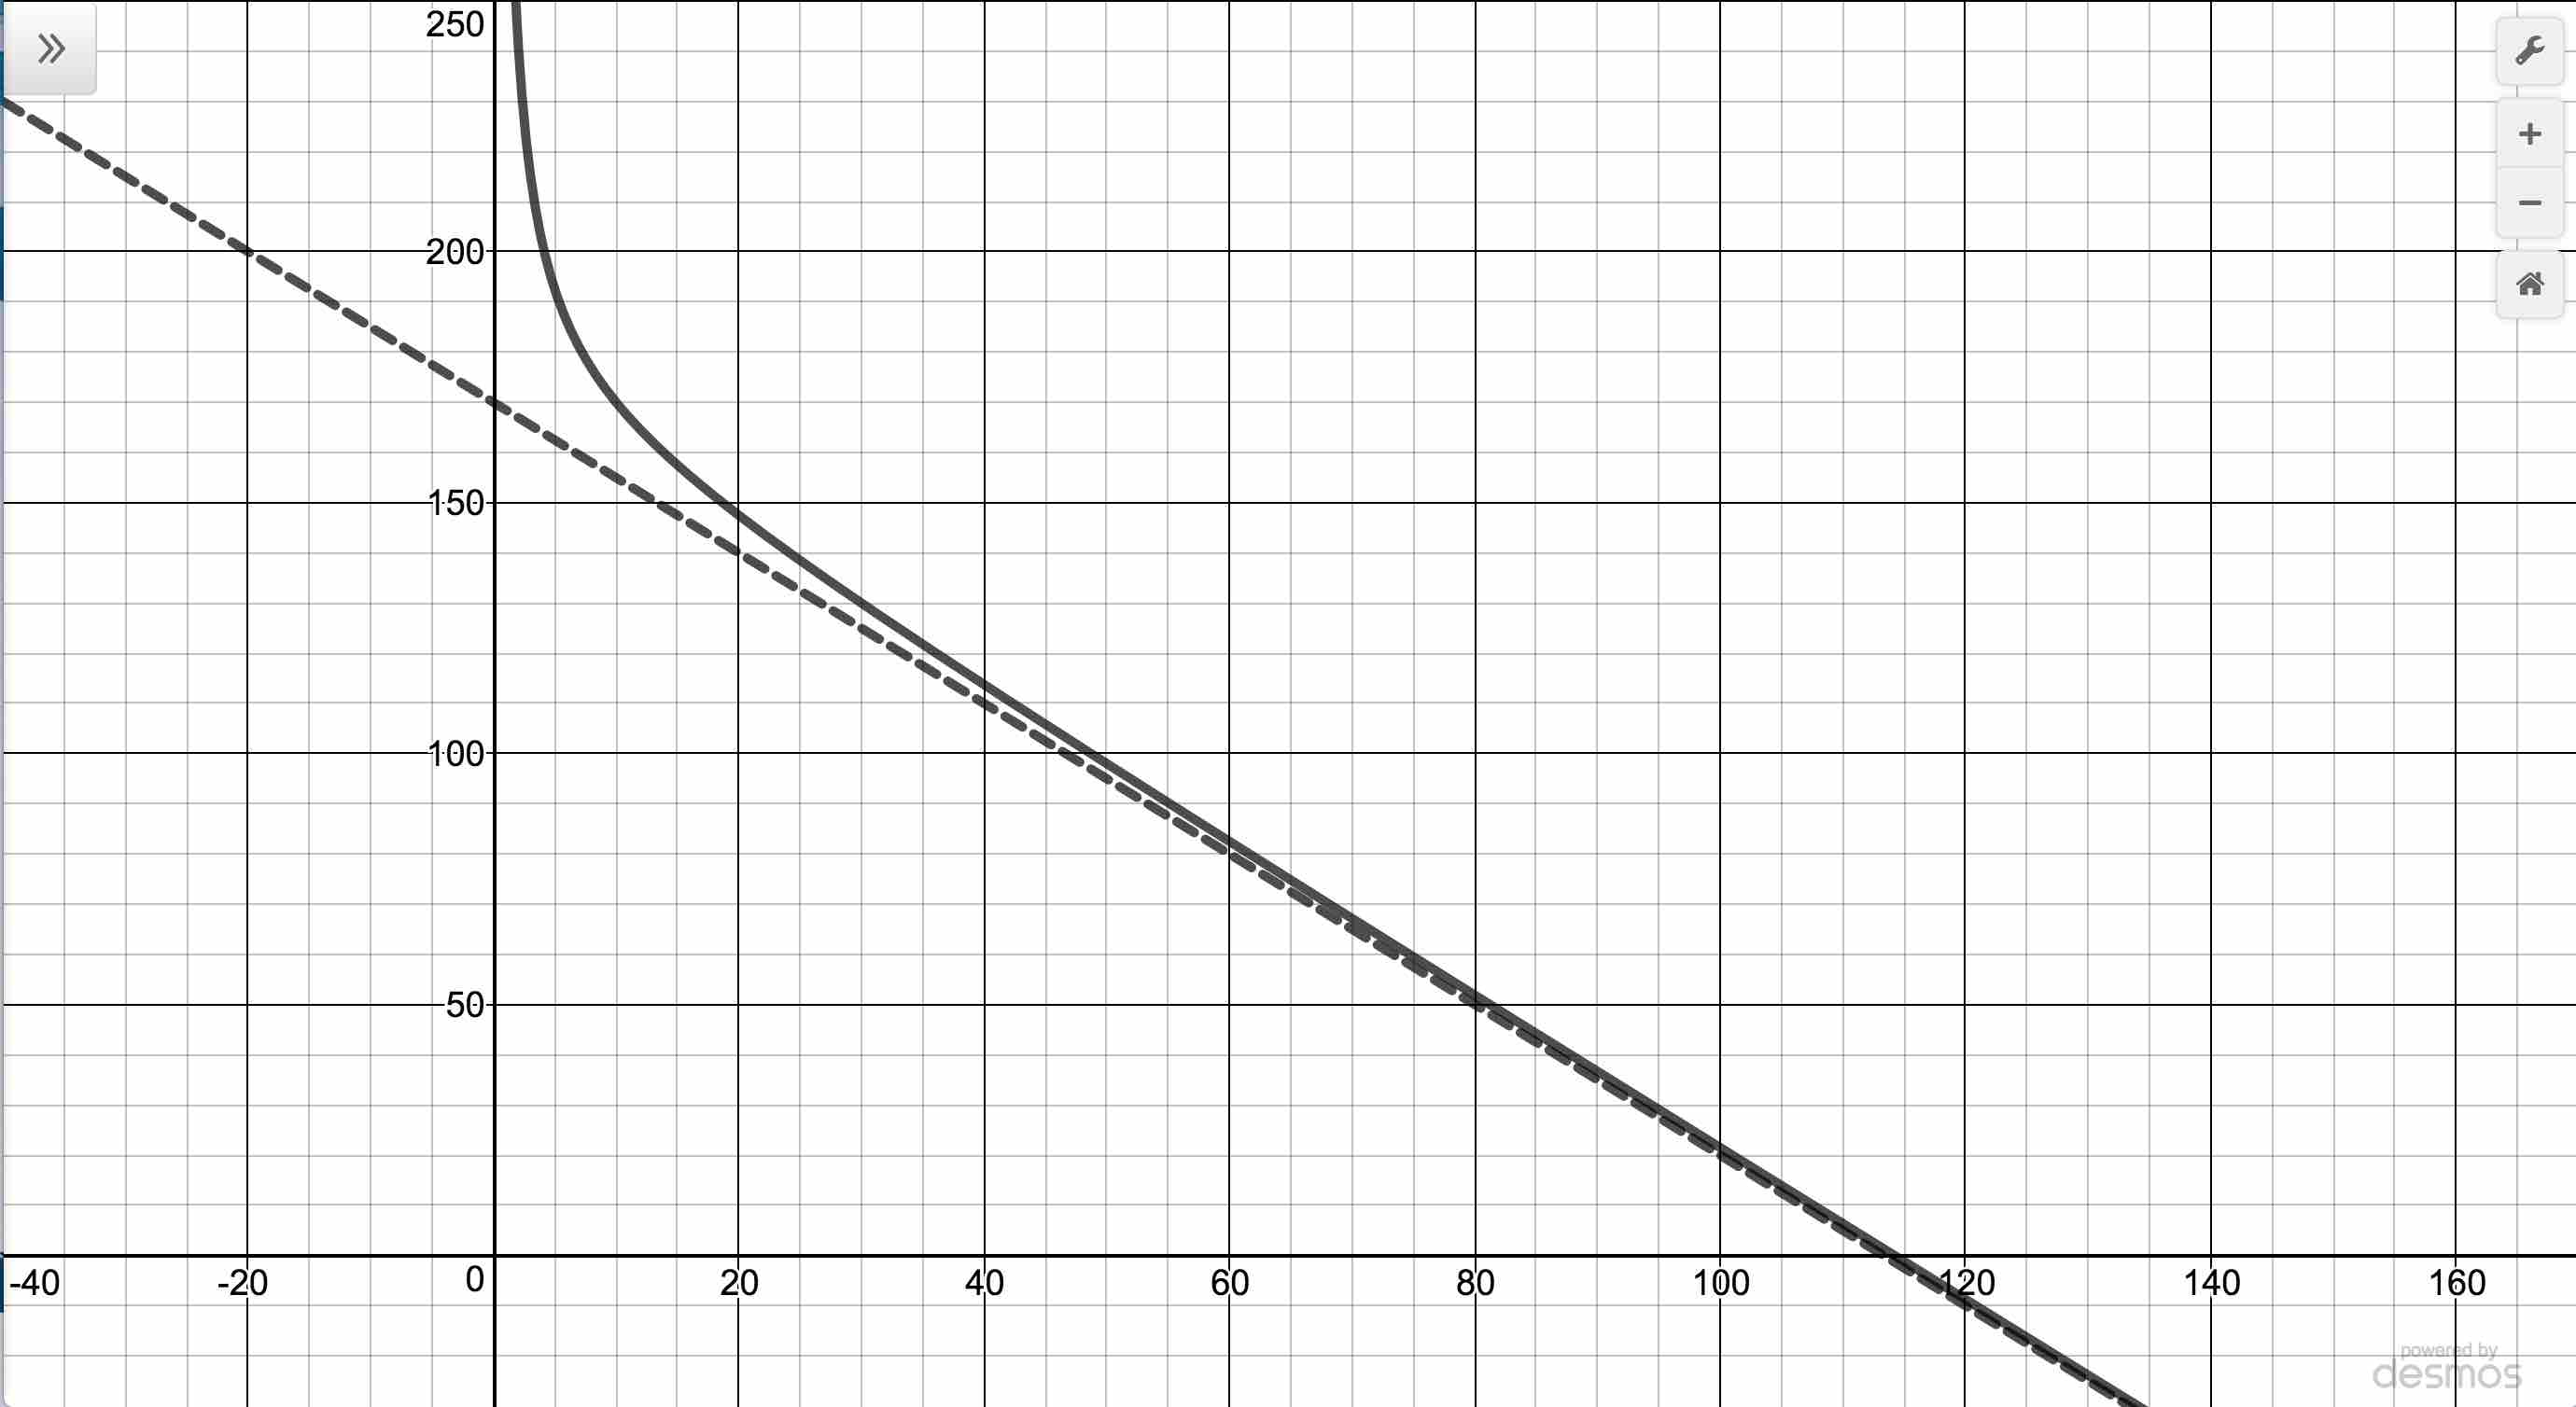
\includegraphics[width=4in]{./IntroRationalGraphics/SAEx06.jpg}

\end{center}

\item The slope of the slant asymptote $y = -1.5x+170$ is $-1.5$.  Since, ostensibly $\overline{P}(x) \approx -1.5 x + 170$, this means that, as we sell more systems, the average profit is decreasing at about a rate of $\$ 1.50$ per system.  If the number $1.5$ sounds familiar to this problem situation, it should.  In Example \ref{PortaBoyDemand} in Section \ref{ConstantandLinearFunctions}, we determined the slope of the demand function to be $-1.5$. In that situation, the $-1.5$ meant that in order to sell an additional system, the price had to drop by $\$ 1.50$.  The fact the average profit is decreasing at more or less this same rate means the loss in profit per system can be attributed to the reduction in price needed to sell each additional system.\footnote{We generalize this result in Exercise \ref{slantyintaverageprofitexercise}.)} \qed

\end{enumerate}


\end{ex}
}

\newpage

\subsection{Exercises}

(Review of Long Division):\footnote{For more review, see Section \ref{polylongdiv}.}  In Exercises \ref{longpolydivreviewfirst} - \ref{longpolydivreviewlast}, use polynomial long division to perform the indicated division.  Write the polynomial in the form $p(x) = d(x)q(x) + r(x)$.

\begin{multicols}{2}
\begin{enumerate}
\item $\left(4x^2+3x-1 \right) \div (x-3)$ \label{longpolydivreviewfirst}
\item $\left(2x^3-x+1 \right) \div \left(x^{2} +x+1 \right)$ 

\setcounter{HW}{\value{enumi}}
\end{enumerate}
\end{multicols}

\begin{multicols}{2}
\begin{enumerate}
\setcounter{enumi}{\value{HW}}

\item $\left(5x^{4} - 3x^{3} + 2x^{2} - 1 \right) \div \left(x^{2} + 4 \right)$
\item $\left(-x^{5} + 7x^{3} - x \right) \div \left(x^{3} - x^{2} + 1 \right)$

\setcounter{HW}{\value{enumi}}
\end{enumerate}
\end{multicols}

\begin{multicols}{2}
\begin{enumerate}
\setcounter{enumi}{\value{HW}}

\item $\left(9x^{3} + 5 \right) \div \left(2x - 3 \right)$
\item $\left(4x^2 - x - 23 \right) \div \left(x^{2} - 1 \right)$ \label{longpolydivreviewlast}

\setcounter{HW}{\value{enumi}}
\end{enumerate}
\end{multicols}


In Exercises \ref{rationaltransfirst} - \ref{rationaltranslast}, given the pair of functions $f$ and $F$, sketch the graph of $y=F(x)$ by starting with the graph of $y = f(x)$ and using Theorem \ref{linearlaurentlgraphs}.   Track at least two points and the asymptotes.  State the domain and range using interval notation.


\begin{multicols}{2}
\begin{enumerate}
\setcounter{enumi}{\value{HW}}
\item $f(x) = \dfrac{1}{x}$,  $F(x) = \dfrac{1}{x-2}+1$ \label{rationaltransfirst}
\item $f(x) =\dfrac{1}{x}$, $F(x) = \dfrac{2x}{x+1}$

\setcounter{HW}{\value{enumi}}
\end{enumerate}
\end{multicols}

\begin{multicols}{2}
\begin{enumerate}
\setcounter{enumi}{\value{HW}}

\item $f(x) =x^{-1}$, $F(x)=4x(2x+1)^{-1}$
\item $f(x) = x^{-2}$, $F(x)=-(x-1)^{-2}+3$  \label{rationaltranslast}

\setcounter{HW}{\value{enumi}}
\end{enumerate}
\end{multicols}


In Exercises \ref{findformulafor1overxgraphfirst} - \ref{findformulafor1overxgraphlast}, find a formula for each function below in the form $F(x) = \dfrac{a}{x-h}+k$.

\begin{multicols}{2}

\begin{enumerate}
\setcounter{enumi}{\value{HW}}

\item $~$ \label{findformulafor1overxgraphfirst}  $y=F(x)$ %$F(x) = \dfrac{1}{x+2}-1$

\begin{mfpic}[15]{-5}{5}{-5}{5}
\axes
\tlabel[cc](5,-0.5){\scriptsize $x$}
\tlabel[cc](0.5,5){\scriptsize $y$}
%\tlabel[cc](-1.5, 0.5){\scriptsize $(-1,0)$}
%\tlabel[cc](-0.5,-1){\scriptsize $\left(0, \frac{1}{2} \right)$}
\xmarks{-4,-3,-2,-1,1,2,3,4}
\ymarks{-4,-3,-2, -1, 1,2,3,4}
\tlpointsep{4pt}
\scriptsize
\axislabels {x}{ {$-4 \hspace{7pt}$} -4, {$-3 \hspace{7pt}$} -3, {$-2 \hspace{7pt}$} -2, {$-1 \hspace{7pt}$} -1, {$1$} 1, {$2$} 2, {$3$} 3, {$4$} 4}
\axislabels {y}{{$-1$} -1,{$1$} 1, {$2$} 2, {$3$} 3, {$4$} 4, {$-2$} -2, {$-3$} -3, {$-4$} -4}
\dashed \polyline{(-4.75,-1), (4.75,-1)}
\dashed \polyline{(-2,-4.75), (-2,4.75)}
\penwd{1.25pt}
\arrow \reverse \arrow \function{-5,-2.25,0.1}{1/(x+2)-1}
\arrow \reverse \arrow \function{-1.83,5,0.1}{1/(x+2)-1}
\point[4pt]{(-1,0), (0,-0.5)}
\tcaption{ \scriptsize $x$-intercept $(-1,0)$, $y$-intercept $\left(0, -\frac{1}{2}\right)$}
\normalsize
\end{mfpic} 



\item $~$ \label{findformulafor1overxgraphlast} $y = F(x)$ %$F(x) = -\dfrac{2}{x-1}+1$

\begin{mfpic}[15]{-5}{5}{-5}{5}
\axes
\tlabel[cc](5,-0.5){\scriptsize $x$}
\tlabel[cc](0.5,5){\scriptsize $y$}
%\tlabel[cc](-1.5, 0.5){\scriptsize $(-1,0)$}
%\tlabel[cc](-0.5,-1){\scriptsize $\left(0, \frac{1}{2} \right)$}
\xmarks{-4,-3,-2,-1,1,2,3,4}
\ymarks{-4,-3,-2, -1, 1,2,3,4}
\tlpointsep{4pt}
\scriptsize
\axislabels {x}{ {$-4 \hspace{7pt}$} -4, {$-3 \hspace{7pt}$} -3, {$-2 \hspace{7pt}$} -2, {$-1 \hspace{7pt}$} -1, {$1$} 1, {$2$} 2, {$3$} 3, {$4$} 4}
\axislabels {y}{{$-1$} -1,{$1$} 1, {$2$} 2, {$3$} 3, {$4$} 4, {$-2$} -2, {$-3$} -3, {$-4$} -4}
\dashed \polyline{(-4.75,1), (4.75,1)}
\dashed \polyline{(1,-4.75), (1,4.75)}
\penwd{1.25pt}
\arrow \reverse \arrow \function{-5,0.45,0.1}{1-2/(x-1)}
\arrow \reverse \arrow \function{1.35,5,0.1}{1-2/(x-1)}
\point[4pt]{(3,0), (0,3)}
\tcaption{ \scriptsize $x$-intercept $(3,0)$, $y$-intercept $\left(0, 3 \right)$}
\normalsize
\end{mfpic} 


\setcounter{HW}{\value{enumi}}

\end{enumerate}

\end{multicols}

\newpage

In Exercises \ref{findformulafor1overxsquaredgraphfirst} - \ref{findformula1overxsquaredgraphlast}, find a formula for each function below in the form $F(x) = \dfrac{a}{(x-h)^2}+k$.


\begin{multicols}{2}

\begin{enumerate}

\setcounter{enumi}{\value{HW}}

\item $~$ \label{findformulafor1overxsquaredgraphfirst} $y = F(x)$ %$F(x) = -\dfrac{4}{(x+2)^2}+4$

\begin{mfpic}[15]{-5}{5}{-5}{5}
\axes
\tlabel[cc](5,-0.5){\scriptsize $x$}
\tlabel[cc](0.5,5){\scriptsize $y$}
%\tlabel[cc](-1.5, 0.5){\scriptsize $(-1,0)$}
%\tlabel[cc](-0.5,-1){\scriptsize $\left(0, \frac{1}{2} \right)$}
\xmarks{-4,-3,-2,-1,1,2,3,4}
\ymarks{-4,-3,-2, -1, 1,2,3,4}
\tlpointsep{4pt}
\scriptsize
\axislabels {x}{ {$-4 \hspace{7pt}$} -4,{$-2 \hspace{7pt}$} -2,  {$1$} 1, {$2$} 2, {$3$} 3, {$4$} 4}
\axislabels {y}{{$-1$} -1,{$1$} 1, {$2$} 2, {$3$} 3, {$4$} 4, {$-2$} -2, {$-3$} -3, {$-4$} -4}
\dashed \polyline{(-4.75,4), (4.75,4)}
\dashed \polyline{(-2,-4.75), (-2,4.75)}
\penwd{1.25pt}
\arrow \reverse \arrow \function{-5,-2.7,0.1}{4-4/((x+2)**2)}
\arrow \reverse \arrow \function{-1.3,5,0.1}{4-4/((x+2)**2)}
\point[4pt]{(-3,0), (-1,0), (0,3)}
\tcaption{\scriptsize $x$-intercepts $(-3,0)$,  $(-1,0)$, $y$-intercept $(0,3)$}
\normalsize
\end{mfpic} 


\item $~$  \label{findformula1overxsquaredgraphlast}$y = F(x)$ %$F(x) = \dfrac{4}{(2x-1)^2}-4$

\begin{mfpic}[15]{-5}{5}{-5}{5}
\axes
\tlabel[cc](5,-0.5){\scriptsize $x$}
\tlabel[cc](0.5,5){\scriptsize $y$}
%\tlabel[cc](-1.5, 0.5){\scriptsize $(-1,0)$}
%\tlabel[cc](-0.5,-1){\scriptsize $\left(0, \frac{1}{2} \right)$}
\xmarks{-4,-3,-2,-1,1,2,3,4}
\ymarks{-4,-3,-2, -1, 1,2,3,4}
\tlpointsep{4pt}
\scriptsize
\axislabels {x}{ {$-4 \hspace{7pt}$} -4, {$-3 \hspace{7pt}$} -3, {$-2 \hspace{7pt}$} -2, {$-1 \hspace{7pt}$} -1, {$1$} 1, {$2$} 2, {$3$} 3, {$4$} 4}
\axislabels {y}{{$-1$} -1,{$1$} 1, {$2$} 2, {$3$} 3, {$4$} 4, {$-2$} -2, {$-4$} -4}
\dashed \polyline{(-4.75,-4), (4.75,-4)}
\dashed \polyline{(0.5,-4.75), (0.5,4.75)}
\penwd{1.25pt}
\arrow \reverse \arrow \function{-5, 0.16, 0.1}{4/((2*x-1)**2) - 4}
\arrow \reverse \arrow \function{0.84, 5, 0.1}{4/((2*x-1)**2) - 4}
\point[4pt]{(0,0), (1,0)}
\tcaption{\scriptsize $x$-intercepts $(0,0)$,  $(1,0)$, Vertical Asymptote:  $x = \frac{1}{2}$}
\normalsize
\end{mfpic} 



\setcounter{HW}{\value{enumi}}

\end{enumerate}

\end{multicols}



In Exercises \ref{alltheasympfirst} - \ref{alltheasymplast}, for the given rational function:

\begin{multicols}{2}
\begin{itemize}

\item State the domain.
\item Identify any vertical asymptotes of the graph.

\end{itemize}
\end{multicols}

\begin{multicols}{2}
\begin{itemize}

\item Identify any holes in the graph.
\item Find the horizontal asymptote, if it exists.

\end{itemize}
\end{multicols}

\begin{multicols}{2}
\begin{itemize}

\item Find the slant asymptote, if it exists.
\item Graph the function using a graphing utility and describe the behavior near the asymptotes.

\end{itemize}
\end{multicols}

\begin{multicols}{3}
\begin{enumerate}
\setcounter{enumi}{\value{HW}}

\item $f(x) = \dfrac{x}{3x - 6}$ \label{alltheasympfirst}
\item $f(x) = \dfrac{3 + 7x}{5 - 2x}$
\item $f(x) = \dfrac{x}{x^{2} + x - 12}$

\setcounter{HW}{\value{enumi}}
\end{enumerate}
\end{multicols}

\begin{multicols}{3}
\begin{enumerate}
\setcounter{enumi}{\value{HW}}

\item $g(t) = \dfrac{t}{t^{2} + 1}$
\item $g(t) = \dfrac{t + 7}{(t + 3)^{2}}$
\item $g(t) = \dfrac{t^{3} + 1}{t^{2} - 1}$

\setcounter{HW}{\value{enumi}}
\end{enumerate}
\end{multicols}

\begin{multicols}{3}
\begin{enumerate}
\setcounter{enumi}{\value{HW}}

\item $r(z) = \dfrac{4z}{z^2+4}$
\item $r(z) = \dfrac{4z}{z^2-4}$
\item $r(z) = \dfrac{z^2-z-12}{z^2+z-6}$

\setcounter{HW}{\value{enumi}}
\end{enumerate}
\end{multicols}

\begin{multicols}{3}
\begin{enumerate}
\setcounter{enumi}{\value{HW}}

\item $f(x) = \dfrac{3x^2-5x-2}{x^2-9}$
\item $f(x) = \dfrac{x^3+2x^2+x}{x^2-x-2}$
\item $f(x) = \dfrac{x^{3} - 3x + 1}{x^{2} + 1}$

\setcounter{HW}{\value{enumi}}
\end{enumerate}
\end{multicols}

\begin{multicols}{3}
\begin{enumerate}
\setcounter{enumi}{\value{HW}}

\item $g(t) = \dfrac{2t^{2} + 5t - 3}{3t + 2}$
\item $g(t) = \dfrac{-t^{3} + 4t}{t^{2} - 9}$
\item \small $g(t) = \dfrac{-5t^{4} - 3t^{3} + t^{2} - 10}{t^{3} - 3t^{2} + 3t - 1}$ \normalsize 

\setcounter{HW}{\value{enumi}}
\end{enumerate}
\end{multicols}


\begin{multicols}{3}
\begin{enumerate}
\setcounter{enumi}{\value{HW}}

\item $r(z) = \dfrac{z^3}{1-z}$
\item $r(z) = \dfrac{18-2z^2}{z^2-9}$
\item $r(z) = \dfrac{z^3-4z^2-4z-5}{z^2+z+1}$ \label{alltheasymplast}


\setcounter{HW}{\value{enumi}}
\end{enumerate}
\end{multicols}

\newpage

\begin{enumerate}
\setcounter{enumi}{\value{HW}}



\item The cost $C(p)$ in dollars to remove $p$\% of the invasive  Ippizuti fish species from Sasquatch Pond is: \[C(p) = \frac{1770p}{100 - p}, \quad 0 \leq p < 100 \]

\begin{enumerate}

\item Find and interpret $C(25)$ and $C(95)$.
\item What does the vertical asymptote at $x = 100$ mean within the context of the problem?  
\item What percentage of the Ippizuti fish can you remove for  \$40000?

\end{enumerate}

\item  \co{In the scenario of  Example \ref{averagevelocityrocketex},} $s(t) = -5t^2+100t$, $0 \leq t \leq 20$ gives the height of a model rocket above the Moon's surface, in feet,  $t$ seconds after liftoff.  For each of the times $t_{0}$ listed below, find and simplify a the formula for the average velocity $\overline{v}(t)$ between $t$ and $t_{0}$ \co{(see Definition \ref{averagevelocitydefn})} and use $\overline{v}(t)$ to find and interpret the instantaneous velocity of the rocket at $t = t_{0}$.

\begin{multicols}{4}

\begin{enumerate}

\item  $t_{0} = 5$

\item $t_{0} = 9$

\item $t_{0} = 10$

\item  $t_{0} = 11$

\end{enumerate}

\end{multicols}


\item \label{squatchpop} The population of Sasquatch in Portage County $t$ years after the year 1803 is modeled by the function \[P(t) = \frac{150t}{t + 15}.\] Find and interpret the horizontal asymptote of the graph of $y = P(t)$ and explain what it means.

\item  The cost in dollars, $C(x)$ to make $x$ dOpi media players is $C(x) = 100x+2000$, $x \geq 0$.  You may wish to review the concepts of fixed and variable costs introduced in  Example \ref{PortaBoyCost} in Section \ref{LinearFunctions}.

\begin{enumerate}

\item  Find a formula for the average cost $\overline{C}(x)$.

\item  Find and interpret $\overline{C}(1)$ and $\overline{C}(100)$.

\item  How many dOpis need to be produced so that the average cost per dOpi is $\$ 200$?

\item  Interpret the behavior of $\overline{C}(x)$ as $x \rightarrow 0^{+}$.  

\item  Interpret the behavior of $\overline{C}(x)$ as $x \rightarrow \infty$.  

\end{enumerate}

\item  \label{averagevariablecostexercise}   This exercise explores the relationships between fixed cost, variable cost, and average cost.  The reader is encouraged to revisit Example \ref{PortaBoyCost} in Section \ref{LinearFunctions} as needed.  Suppose the cost in dollars $C(x)$ to make $x$ items is given by $C(x) = mx + b$ where $m$ and $b$ are positive real numbers.

\begin{enumerate}

\item  Show the fixed cost (the money spent even if no items are made) is $b$.
\item  Show the variable cost (the increase in cost per item made) is $m$.
\item  Find a formula for the average cost when making $x$ items, $\overline{C}(x)$.
\item  Show $\overline{C}(x) > m$ for all $x>0$ and, moreover,   $\overline{C}(x)  \rightarrow m^{+}$ as $x \rightarrow \infty$. 
\item  Interpret $\overline{C}(x)  \rightarrow m^{+}$ both geometrically and in terms of fixed, variable, and average costs.

\end{enumerate}

\item  \label{slantyintaverageprofitexercise} Suppose the price-demand function for a particular product is given by $p(x) = mx + b$  where $x$ is the number of items made and sold for $p(x)$ dollars.  Here,  $m<0$ and $b>0$.  If the cost (in dollars) to make $x$ of these products is also a linear  function $C(x)$, show that the graph of the average profit function $\overline{P}(x)$ has a slant asymptote with slope $m$ and interpret.

\item In Exercise \ref{circuitexercisepoly} in Section \ref{GraphsofPolynomials}, we fit a few polynomial models to the following electric circuit data. The circuit was built with a variable resistor.  For each of the following resistance values (measured in kilo-ohms, $k \Omega$),  the corresponding power to the load (measured in milliwatts, $mW$) is given below.\footnote{The authors wish to thank Don Anthan and Ken White of Lakeland Community College for devising this problem and generating the accompanying data set.}


\smallskip

\noindent \begin{tabular}{|l|r|r|r|r|r|r|} \hline
Resistance: ($k \Omega$) & 1.012 & 2.199 & 3.275 & 4.676 & 6.805 & 9.975 \\ \hline
Power: ($mW$) & 1.063 & 1.496 & 1.610 & 1.613 & 1.505 & 1.314 \\ \hline
\end{tabular}

\smallskip

\noindent Using some fundamental laws of circuit analysis mixed with a healthy dose of algebra, we can derive the actual formula relating power $P(x)$ to resistance $x$:   \[P(x) = \frac{25x}{(x + 3.9)^2}, \quad x \geq 0.\]

\begin{enumerate}

\item Graph the data along with the function $y = P(x)$ using a graphing utility.

\item Use a graphing utility to approximate the maximum power that can be delivered to the load.  What is the corresponding resistance value?

\item Find and interpret the end behavior of $P(x)$ as $x \rightarrow \infty$.

\end{enumerate}


\item  Let $f(x) = \dfrac{ax^2-c}{x+3}$.  Find values  for $a$ and  $c$ so  the graph of $f$ has a hole  at $(-3, 12)$.

\item  Let  $f(x) = \dfrac{ax^{n} -4}{2x^2+1}$.

\begin{enumerate}

\item  Find values for $a$ and $n$ so the graph of $y = f(x)$  has the horizontal asymptote $y = 3$.

\item  Find values for $a$ and $n$ so the graph of  $y=f(x)$ has the slant asymptote $y = 5x$.

\end{enumerate}


\item  Suppose $p$ is a polynomial function and $a$ is a real number.  Define $r(x)= \dfrac{p(x) - p(a)}{x-a}$.  Use the Factor Theorem\co{, Theorem \ref{factorthm}}, to prove the graph of $y = r(x)$ has a hole at $x =a$.  


\item \label{laurentarcexercise}For each function $f(x)$ listed below, compute the average rate of change over the indicated interval.\co{\footnote{See Definition \ref{arc} in Section \ref{AverageRateofChange} for a review of this concept, as needed.}}  What trends do you observe?  How do your answers manifest themselves graphically?  How do you results compare with those of Exercise \ref{monomialarcexercise} in Section \ref{GraphsofPolynomials}?

\vspace*{-0.2in}

\[ \begin{array}{|r||c|c|c|c|}  \hline

 f(x) &  [0.9, 1.1] & [0.99, 1.01] &[0.999, 1.001] & [0.9999, 1.0001]  \\ \hline
 x^{-1} &&&&   \\  \hline
 x^{-2} &&&&    \\  \hline
 x^{-3} &&&&   \\  \hline
 x^{-4} &&&&   \\  \hline
\end{array} \]

\item \index{Learning Curve Equation} \index{Thurstone, Louis Leon} In his now famous 1919 dissertation \underline{The Learning Curve Equation}, Louis Leon Thurstone presents a rational function which models the number of words a person can type in four minutes as a function of the number of pages of practice one has completed.\footnote{This paper, which is now in the public domain and can be found  \href{http://bit.ly/2uNaUBa}{\underline{here}}, is from a bygone era when students at business schools took typing classes on manual typewriters.} Using his original notation and original language, we have $Y = \frac{L(X + P)}{(X + P) + R}$ where $L$ is the predicted practice limit in terms of speed units, $X$ is pages written, $Y$ is writing speed in terms of words in four minutes, $P$ is equivalent previous practice in terms of pages and $R$ is the rate of learning. In Figure 5 of the paper, he graphs a scatter plot and the curve $Y = \frac{216(X + 19)}{X + 148}$.  Discuss this equation with your classmates.  How would you update the notation?  Explain what the horizontal asymptote of the graph means.  You should take some time to look at the original paper. Skip over the computations you don't understand yet and try to get a sense of the time and place in which the study was conducted.

\end{enumerate}

\newpage

\subsection{Answers}

\begin{enumerate}
\item $4x^2+3x-1 = (x-3)(4x+15) + 44$
\item $2x^3-x+1 = \left(x^2+x+1\right)(2x-2)+(-x+3)$
\item $5x^{4} - 3x^{3} + 2x^{2} - 1 = \left(x^{2} + 4 \right) \left(5x^{2} - 3x - 18 \right) + (12x + 71)$
\item $-x^{5} + 7x^{3} - x = \left(x^{3} - x^{2} + 1 \right) \left(-x^{2} - x + 6 \right) + \left(7x^{2} - 6 \right)$
\item $9x^{3} + 5 =(2x - 3) \left(\frac{9}{2}x^{2} + \frac{27}{4}x + \frac{81}{8} \right) + \frac{283}{8}$
\item $4x^2 - x - 23 = \left(x^{2} - 1 \right)(4) + (-x - 19)$
\setcounter{HW}{\value{enumi}}
\end{enumerate}


\begin{multicols}{2}
\begin{enumerate}
\setcounter{enumi}{\value{HW}}

\item $F(x) = \dfrac{1}{x-2}+1$ \\ [10pt]
Domain: $(-\infty, 2) \cup (2, \infty)$ \\ 
Range: $(-\infty, 1) \cup (1, \infty)$ \\
Vertical asymptote:  $x = 2$\\
Horizontal asymptote:  $y = 1$ \\

\begin{mfpic}[15]{-5}{5}{-5}{5}
\axes
\tlabel[cc](5,-0.5){\scriptsize $x$}
\tlabel[cc](0.5,5){\scriptsize $y$}
%\tlabel[cc](-1.5, 0.5){\scriptsize $(-1,0)$}
%\tlabel[cc](-0.5,-1){\scriptsize $\left(0, \frac{1}{2} \right)$}
\xmarks{-4,-3,-2,-1,1,2,3,4}
\ymarks{-4,-3,-2, -1, 1,2,3,4}
\tlpointsep{4pt}
\scriptsize
\axislabels {x}{ {$-4 \hspace{7pt}$} -4, {$-3 \hspace{7pt}$} -3, {$-2 \hspace{7pt}$} -2, {$-1 \hspace{7pt}$} -1, {$1$} 1, {$2$} 2, {$3$} 3, {$4$} 4}
\axislabels {y}{{$-1$} -1,{$1$} 1, {$2$} 2, {$3$} 3, {$4$} 4, {$-2$} -2, {$-3$} -3, {$-4$} -4}
\dashed \polyline{(-4.75,1), (4.75,1)}
\dashed \polyline{(2,-4.75), (2,4.75)}
\penwd{1.25pt}
\arrow \reverse \arrow \function{-5,1.8,0.1}{1+1/(x-2)}
\arrow \reverse \arrow \function{2.3,5,0.1}{1+1/(x-2)}
\point[4pt]{(1,0), (3,2)}
\normalsize
\end{mfpic} 


\vfill

\columnbreak

\item $F(x) = \dfrac{2x}{x+1} = \dfrac{-2}{x+1}+2$\\ [10pt]
Domain: $(-\infty, -1) \cup (-1, \infty)$ \\ 
Range: $(-\infty, 2) \cup (2, \infty)$ \\
Vertical asymptote:  $x = -1$\\
Horizontal asymptote:  $y = 2$ \\

\begin{mfpic}[15]{-5}{5}{-5}{5}
\axes
\tlabel[cc](5,-0.5){\scriptsize $x$}
\tlabel[cc](0.5,5){\scriptsize $y$}
%\tlabel[cc](-1.5, 0.5){\scriptsize $(-1,0)$}
%\tlabel[cc](-0.5,-1){\scriptsize $\left(0, \frac{1}{2} \right)$}
\xmarks{-4,-3,-2,-1,1,2,3,4}
\ymarks{-4,-3,-2, -1, 1,2,3,4}
\tlpointsep{4pt}
\scriptsize
\axislabels {x}{ {$-4 \hspace{7pt}$} -4, {$-3 \hspace{7pt}$} -3, {$-2 \hspace{7pt}$} -2, {$-1 \hspace{7pt}$} -1, {$1$} 1, {$2$} 2, {$3$} 3, {$4$} 4}
\axislabels {y}{{$1$} 1, {$2$} 2, {$3$} 3, {$4$} 4}
\dashed \polyline{(-4.75,2), (4.75,2)}
\dashed \polyline{(-1,-4.75), (-1,4.75)}
\penwd{1.25pt}
\arrow \reverse \arrow \function{-5,-1.7,0.1}{2x/(x+1)}
\arrow \reverse \arrow \function{-0.7,5,0.1}{2x/(x+1)}
\point[4pt]{(0,0), (-2,4)}
\normalsize
\end{mfpic} 

\setcounter{HW}{\value{enumi}}
\end{enumerate}
\end{multicols}



\begin{multicols}{2}
\begin{enumerate}
\setcounter{enumi}{\value{HW}}

\item $F(x)=4x(2x+1)^{-1} = \dfrac{4x}{2x+1} = \dfrac{-1}{x+\frac{1}{2}}+2$ \\ [10pt]
Domain: $\left(-\infty, -\frac{1}{2} \right) \cup \left(-\frac{1}{2},  \infty \right)$ \\ 
Range: $(-\infty, 2) \cup (2, \infty)$ \\
Vertical asymptote:  $y= 2$\\
Horizontal asymptote:  $x  = -\frac{1}{2}$ \\

\begin{mfpic}[15]{-5}{5}{-5}{5}
\axes
\tlabel[cc](5,-0.5){\scriptsize $x$}
\tlabel[cc](0.5,5){\scriptsize $y$}
%\tlabel[cc](-1.5, 0.5){\scriptsize $(-1,0)$}
%\tlabel[cc](-0.5,-1){\scriptsize $\left(0, \frac{1}{2} \right)$}
\xmarks{-4,-3,-2,-1,1,2,3,4}
\ymarks{-4,-3,-2, -1, 1,2,3,4}
\tlpointsep{4pt}
\scriptsize
\axislabels {x}{ {$-4 \hspace{7pt}$} -4, {$-3 \hspace{7pt}$} -3, {$-2 \hspace{7pt}$} -2, {$-1 \hspace{7pt}$} -1, {$1$} 1, {$2$} 2, {$3$} 3, {$4$} 4}
\axislabels {y}{{$1$} 1, {$2$} 2, {$3$} 3, {$4$} 4}
\dashed \polyline{(-4.75,2), (4.75,2)}
\dashed \polyline{(-0.5,-4.75), (-0.5,4.75)}
\penwd{1.25pt}
\arrow \reverse \arrow \function{-5,-0.84,0.1}{4*x/(2*x+1)}
\arrow \reverse \arrow \function{-0.35,5,0.1}{4*x/(2*x+1)}
\point[4pt]{(-1.5,3), (0.5,1)}
\normalsize
\end{mfpic} 


\vfill

\columnbreak

\item $F(x)=-(x-1)^{-2}+3 = \dfrac{-1}{(x-1)^2} + 3$\\[10pt]
Domain: $(-\infty, 1) \cup (1, \infty)$ \\ 
Range: $(-\infty, 3) \cup (3, \infty)$ \\
Vertical asymptote:  $x = 1$\\
Horizontal asymptote:  $y = 3$ \\

\begin{mfpic}[15]{-5}{5}{-5}{5}
\axes
\tlabel[cc](5,-0.5){\scriptsize $x$}
\tlabel[cc](0.5,5){\scriptsize $y$}
%\tlabel[cc](-1.5, 0.5){\scriptsize $(-1,0)$}
%\tlabel[cc](-0.5,-1){\scriptsize $\left(0, \frac{1}{2} \right)$}
\xmarks{-4,-3,-2,-1,1,2,3,4}
\ymarks{-4,-3,-2, -1, 1,2,3,4}
\tlpointsep{4pt}
\scriptsize
\axislabels {x}{ {$-4 \hspace{7pt}$} -4, {$-3 \hspace{7pt}$} -3, {$-2 \hspace{7pt}$} -2, {$-1 \hspace{7pt}$} -1,  {$2$} 2, {$3$} 3, {$4$} 4}
\axislabels {y}{{$1$} 1, {$2$} 2, {$3$} 3, {$4$} 4, {$-1$} -1, {$-2$} -2, {$-3$} -3, {$-4$} -4}
\dashed \polyline{(-4.75,3), (4.75,3)}
\dashed \polyline{(1,-4.75), (1,4.75)}
\penwd{1.25pt}
\arrow \reverse \arrow \function{-5,0.64,0.1}{3-1/((x-1)**2)}
\arrow \reverse \arrow \function{1.36,5,0.1}{3-1/((x-1)**2)}
\point[4pt]{(0,2), (2,2)}
\normalsize
\end{mfpic} 

\setcounter{HW}{\value{enumi}}
\end{enumerate}
\end{multicols}

\begin{multicols}{2}
\begin{enumerate}
\setcounter{enumi}{\value{HW}}

\item $F(x) = \dfrac{1}{x+2}-1$

\item  $F(x) = \dfrac{-2}{x-1}+1$

\setcounter{HW}{\value{enumi}}
\end{enumerate}
\end{multicols}


\begin{multicols}{2}

\begin{enumerate}

\setcounter{enumi}{\value{HW}}

\item  $F(x) = \dfrac{-4}{(x+2)^2}+4$  \vphantom{$F(x) = \dfrac{1}{\left(x-\frac{1}{2}\right)^2}-4$}

\item $F(x) = \dfrac{1}{\left(x-\frac{1}{2}\right)^2}-4$

\setcounter{HW}{\value{enumi}}
\end{enumerate}
\end{multicols}



\begin{multicols}{2}
\begin{enumerate} 
\setcounter{enumi}{\value{HW}}

\item $f(x) = \dfrac{x}{3x - 6}$ \vphantom{$\dfrac{7x}{7x}$}\\ 
Domain: $(-\infty, 2) \cup (2, \infty)$\\
Vertical asymptote: $x = 2$\\
As $x \rightarrow 2^{-}, f(x) \rightarrow -\infty$\\
As $x \rightarrow 2^{+}, f(x) \rightarrow \infty$\\
No holes in the graph\\
Horizontal asymptote: $y = \frac{1}{3}$ \\
As $x \rightarrow -\infty, f(x) \rightarrow \frac{1}{3}^{-}$\\
As $x \rightarrow \infty, f(x) \rightarrow \frac{1}{3}^{+}$\\

\vfill

\columnbreak

\item $f(x) = \dfrac{3 + 7x}{5 - 2x}$\\
Domain: $(-\infty, \frac{5}{2}) \cup (\frac{5}{2}, \infty)$\\
Vertical asymptote: $x = \frac{5}{2}$\\
As $x \rightarrow \frac{5}{2}^{-}, f(x) \rightarrow \infty$\\
As $x \rightarrow \frac{5}{2}^{+}, f(x) \rightarrow -\infty$\\
No holes in the graph\\
Horizontal asymptote: $y = -\frac{7}{2}$ \\
As $x \rightarrow -\infty, f(x) \rightarrow -\frac{7}{2}^{+}$\\
As $x \rightarrow \infty, f(x) \rightarrow -\frac{7}{2}^{-}$\\

\setcounter{HW}{\value{enumi}}
\end{enumerate}
\end{multicols}

\begin{multicols}{2}
\begin{enumerate}
\setcounter{enumi}{\value{HW}}

\item $f(x) = \dfrac{x}{x^{2} + x - 12} = \dfrac{x}{(x + 4)(x - 3)}$\\
Domain: $(-\infty, -4) \cup (-4, 3) \cup (3, \infty)$\\
Vertical asymptotes: $x = -4, x = 3$\\
As $x \rightarrow -4^{-}, f(x) \rightarrow -\infty$\\
As $x \rightarrow -4^{+}, f(x) \rightarrow \infty$\\
As $x \rightarrow 3^{-}, f(x) \rightarrow -\infty$\\
As $x \rightarrow 3^{+}, f(x) \rightarrow \infty$\\
No holes in the graph\\
Horizontal asymptote: $y = 0$ \\
As $x \rightarrow -\infty, f(x) \rightarrow 0^{-}$\\
As $x \rightarrow \infty, f(x) \rightarrow 0^{+}$\\

\vfill

\columnbreak


\item $g(t) = \dfrac{t}{t^{2} + 1}$\\
Domain: $(-\infty, \infty)$\\
No vertical asymptotes\\
No holes in the graph\\
Horizontal asymptote: $y = 0$ \\
As $t \rightarrow -\infty, g(t) \rightarrow 0^{-}$\\
As $t \rightarrow \infty, g(t) \rightarrow 0^{+}$\\

\setcounter{HW}{\value{enumi}}
\end{enumerate}
\end{multicols}

\begin{multicols}{2}
\begin{enumerate}
\setcounter{enumi}{\value{HW}}

\item $g(t) = \dfrac{t + 7}{(t + 3)^{2}}$ \vphantom{$\dfrac{t^{3}}{t^{2}}$}\\
Domain: $(-\infty, -3) \cup (-3, \infty)$\\
Vertical asymptote: $t = -3$\\
As $t \rightarrow -3^{-}, g(t) \rightarrow \infty$\\
As $t \rightarrow -3^{+}, g(t) \rightarrow \infty$\\
No holes in the graph\\
Horizontal asymptote: $y = 0$ \\
\footnote{This is hard to see on the calculator, but trust me, the graph is below the $t$-axis to the left of $t = -7$.}As $t \rightarrow -\infty, g(t) \rightarrow 0^{-}$\\
As $t \rightarrow \infty, g(t) \rightarrow 0^{+}$\\

\vfill

\columnbreak

\item $g(t) = \dfrac{t^{3} + 1}{t^{2} - 1} = \dfrac{t^{2} - t+ 1}{t-1}$\\
Domain: $(-\infty, -1) \cup (-1, 1) \cup (1, \infty)$\\
Vertical asymptote: $t = 1$\\
As $t \rightarrow 1^{-}, g(t) \rightarrow -\infty$\\
As $t \rightarrow 1^{+}, g(t) \rightarrow \infty$\\
Hole at $(-1, -\frac{3}{2})$\\
Slant asymptote: $y=t$  \\
As $t \rightarrow -\infty$, the graph is below $y=t$\\
As $t \rightarrow \infty$, the graph is above $y=t$\\

\setcounter{HW}{\value{enumi}}
\end{enumerate}
\end{multicols}

\begin{multicols}{2}
\begin{enumerate}
\setcounter{enumi}{\value{HW}}

\item $r(z) = \dfrac{4z}{z^{2} + 4}$\\
Domain: $(-\infty,  \infty)$\\
No vertical asymptotes \\
No holes in the graph\\
Horizontal asymptote: $y = 0$ \\
As $z \rightarrow -\infty, r(z) \rightarrow 0^{-}$\\
As $z \rightarrow \infty, r(z) \rightarrow 0^{+}$\\


\vfill

\columnbreak

\item $r(z) = \dfrac{4z}{z^{2} -4} = \dfrac{4z}{(z + 2)(z - 2)}$\\
Domain: $(-\infty, -2) \cup (-2, 2) \cup (2, \infty)$\\
Vertical asymptotes: $z = -2, z = 2$\\
As $z \rightarrow -2^{-}, r(z) \rightarrow -\infty$\\
As $z \rightarrow -2^{+}, r(z) \rightarrow \infty$\\
As $z \rightarrow 2^{-}, r(z) \rightarrow -\infty$\\
As $z \rightarrow 2^{+}, r(z) \rightarrow \infty$\\
No holes in the graph\\
Horizontal asymptote: $y = 0$ \\
As $z \rightarrow -\infty, r(z) \rightarrow 0^{-}$\\
As $z \rightarrow \infty, r(z) \rightarrow 0^{+}$\\

\setcounter{HW}{\value{enumi}}
\end{enumerate}
\end{multicols}

\begin{multicols}{2}
\begin{enumerate}
\setcounter{enumi}{\value{HW}}

\item $r(z) = \dfrac{z^2-z-12}{z^{2} +z - 6} = \dfrac{z-4}{z - 2}$\\
Domain: $(-\infty, -3) \cup (-3, 2) \cup (2, \infty)$\\
Vertical asymptote: $z = 2$\\
As $z \rightarrow 2^{-}, r(z) \rightarrow \infty$\\
As $z \rightarrow 2^{+}, r(z) \rightarrow -\infty$\\
Hole at $\left(-3, \frac{7}{5} \right)$ \\
Horizontal asymptote: $y = 1$ \\
As $z \rightarrow -\infty, r(z) \rightarrow 1^{+}$\\
As $z \rightarrow \infty, r(z) \rightarrow 1^{-}$\\


\vfill

\columnbreak

\item $f(x) = \dfrac{3x^2-5x-2}{x^{2} -9} = \dfrac{(3x+1)(x-2)}{(x + 3)(x - 3)}$\\
Domain: $(-\infty, -3) \cup (-3, 3) \cup (3, \infty)$\\
Vertical asymptotes: $x = -3, x = 3$\\
As $x \rightarrow -3^{-}, f(x) \rightarrow \infty$\\
As $x \rightarrow -3^{+}, f(x) \rightarrow -\infty$\\
As $x \rightarrow 3^{-}, f(x) \rightarrow -\infty$\\
As $x \rightarrow 3^{+}, f(x) \rightarrow \infty$\\
No holes in the graph\\
Horizontal asymptote: $y = 3$ \\
As $x \rightarrow -\infty, f(x) \rightarrow 3^{+}$\\
As $x \rightarrow \infty, f(x) \rightarrow 3^{-}$\\

\setcounter{HW}{\value{enumi}}
\end{enumerate}
\end{multicols}

\begin{multicols}{2}
\begin{enumerate}
\setcounter{enumi}{\value{HW}}


\item $f(x) = \dfrac{x^3+2x^2+x}{x^{2} -x-2} = \dfrac{x(x+1)}{x - 2}$\\
Domain: $(-\infty, -1) \cup (-1, 2) \cup (2, \infty)$\\
Vertical asymptote: $x = 2$\\
As $x \rightarrow 2^{-}, f(x) \rightarrow -\infty$\\
As $x \rightarrow 2^{+}, f(x) \rightarrow \infty$\\
Hole at $(-1,0)$ \\
Slant asymptote: $y=x+3$ \\
As $x \rightarrow -\infty$, the graph is below $y=x+3$\\
As $x \rightarrow \infty$, the graph is above $y=x+3$\\

\vfill

\columnbreak

\item $f(x) = \dfrac{x^3-3x+1}{x^2+1}$\\
Domain: $(-\infty, \infty)$\\
No vertical asymptotes \\
No holes in the graph \\
Slant asymptote: $y=x$ \\
As $x \rightarrow -\infty$, the graph is above $y=x$ \\
As $x \rightarrow \infty$, the graph is below $y=x$  \\


\setcounter{HW}{\value{enumi}}
\end{enumerate}
\end{multicols}


\begin{multicols}{2}
\begin{enumerate}
\setcounter{enumi}{\value{HW}}

\item $g(t) = \dfrac{2t^{2} + 5t - 3}{3t + 2}$\\
Domain: $\left(-\infty, -\frac{2}{3}\right) \cup \left(-\frac{2}{3}, \infty\right)$\\
Vertical asymptote: $t = -\frac{2}{3}$\\
As $t \rightarrow -\frac{2}{3}^{-}, g(t) \rightarrow \infty$\\
As $t \rightarrow -\frac{2}{3}^{+}, g(t) \rightarrow -\infty$\\
No holes in the graph \\
Slant asymptote:  $y = \frac{2}{3}t + \frac{11}{9}$ \\
As $t \rightarrow  -\infty$, the graph is above \small $y = \frac{2}{3}t + \frac{11}{9}$\\
\normalsize As $t \rightarrow \infty$, the graph is below \small $y = \frac{2}{3}t + \frac{11}{9}$ \normalsize \\

\vfill

\columnbreak

\item $g(t) = \dfrac{-t^{3} + 4t}{t^{2} - 9} = \dfrac{-t^{3} + 4t}{(t-3)(t+3)} $\\
Domain: $(-\infty, -3) \cup (-3, 3) \cup (3, \infty)$\\
Vertical asymptotes: $t = -3$, $t=3$\\
As $t \rightarrow -3^{-}, g(t) \rightarrow \infty$\\
As $t \rightarrow -3^{+}, g(t) \rightarrow -\infty$\\
As $t \rightarrow 3^{-}, g(t) \rightarrow \infty$\\
As $t \rightarrow 3^{+}, g(t) \rightarrow -\infty$\\
No holes in the graph \\
Slant asymptote: $y=-t$ \\
As $t \rightarrow -\infty$, the graph is above $y=-t$\\
As $t \rightarrow \infty$, the graph is below $y=-t$\\


\setcounter{HW}{\value{enumi}}
\end{enumerate}
\end{multicols}

\begin{multicols}{2}
\begin{enumerate}
\setcounter{enumi}{\value{HW}}

\item \small $g(t) = \dfrac{-5t^{4} - 3t^{3} + t^{2} - 10}{t^{3} - 3t^{2} + 3t - 1} \\ \phantom{g(t)} = \dfrac{-5t^{4} - 3t^{3} + t^{2} - 10}{(t-1)^3} $ \normalsize \\
Domain: $(-\infty, 1) \cup (1, \infty)$\\
Vertical asymptotes: $t = 1$\\
As $t \rightarrow 1^{-}, g(t) \rightarrow \infty$\\
As $t \rightarrow 1^{+}, g(t) \rightarrow -\infty$\\
No holes in the graph \\
Slant asymptote: $y=-5t-18$ \\
 \small  As $t \rightarrow -\infty$, the graph is above $y=-5t-18$ \normalsize\\
 \small  As $t \rightarrow \infty$, the graph is below $y=-5t-18$ \normalsize \\
 
 \vfill
 
 \columnbreak

\item $r(z) = \dfrac{z^3}{1-z}$\\
Domain: $(-\infty, 1) \cup (1, \infty)$\\
Vertical asymptote: $z=1$\\
As $z \rightarrow 1^{-}, r(z) \rightarrow \infty$\\
As $z \rightarrow 1^{+}, r(z) \rightarrow -\infty$\\
No holes in the graph \\
No horizontal or slant asymptote \\
As $z \rightarrow -\infty$, $r(z) \rightarrow -\infty$\\
As $z \rightarrow \infty$, $r(z) \rightarrow -\infty$\\


\setcounter{HW}{\value{enumi}}
\end{enumerate}
\end{multicols}

\begin{multicols}{2}
\begin{enumerate}
\setcounter{enumi}{\value{HW}}

\item $r(z) = \dfrac{18-2z^2}{z^2-9} = -2$\\
Domain: $(-\infty, -3) \cup (-3,3) \cup (3, \infty)$\\
No vertical asymptotes \\
Holes in the graph at $(-3,-2)$ and $(3,-2)$ \\
Horizontal asymptote $y = -2$ \\
As $z \rightarrow \pm \infty$, $r(z) = -2$ \\

\vfill
\columnbreak

\item $r(z) = \dfrac{z^3-4z^2-4z-5}{z^2+z+1} = z-5$\\
Domain: $(-\infty, \infty)$\\
No vertical asymptotes \\
No holes in the graph \\
Slant asymptote:  $y = z-5$ \\
$r(z) = z-5$ everywhere. \\


\setcounter{HW}{\value{enumi}}
\end{enumerate}
\end{multicols}

\begin{enumerate}
\setcounter{enumi}{\value{HW}}


\item \begin{enumerate}

\item $C(25) = 590$ means it costs \$590 to remove 25\% of the fish and and $C(95)= 33630$ means it would cost \$33630 to remove 95\% of the fish from the pond.
\item The vertical asymptote at $x = 100$ means that as we try to remove 100\% of the fish from the pond, the cost increases without bound; i.e., it's impossible to remove all of the fish.  
\item For \$40000 you could remove about 95.76\% of the fish.

\end{enumerate}

\item  \begin{enumerate}

\item  $\overline{v}(t) = \frac{s(t) - s(5)}{t - 5} = \frac{-5t^2+100t-375}{t-5} = -5t+75$, $t \neq 5$.  The instantaneous velocity of the rocket when $t_{0} = 5$ is $-5(5)+75 = 50$ meaning it is traveling $50$ feet per second upwards.

\item  $\overline{v}(t) = \frac{s(t) - s(9)}{t - 9} = \frac{-5t^2+100t-495}{t-9} = -5t+55$, $t \neq 9$.  The instantaneous velocity of the rocket when $t_{0} = 9$ is $-5(9)+55 = 10$, so the rocket has slowed to $10$ feet per second (but still heading up.)

\item $\overline{v}(t) = \frac{s(t) - s(10)}{t - 10} = \frac{-5t^2+100t-495}{t-10} = -5t+50$, $t \neq 10$.  The instantaneous velocity of the rocket when $t_{0} = 10$ is $-5(10)+50 = 0$, so the rocket has momentarily stopped!  \co{In Example \ref{ARCRocketExample}, we learned t}The rocket reaches its maximum height when $t = 10$ seconds, which means the rocket must change direction from heading up to coming back down, so it makes sense that for this instant, its velocity is $0$.

\item  $\overline{v}(t) = \frac{s(t) - s(11)}{t - 11} = \frac{-5t^2+100t-495}{t-11} = -5t+45$, $t \neq 11$.  The instantaneous velocity of the rocket when $t_{0} = 11$ is $-5(11)+45 = -10$ meaning the rocket has, indeed, changed direction and is heading downwards at a rate of $10$ feet per second.  (Note the symmetry here between this answer and our answer when $t=9$.)

\end{enumerate}

\item The horizontal asymptote of the graph of $P(t) = \frac{150t}{t + 15}$ is $y = 150$ and it means that the model predicts the population of Sasquatch in Portage County will never exceed 150.

\item  \begin{enumerate}

\item $\overline{C}(x) = \frac{100x+2000}{x} = 100 + \frac{2000}{x}$, $x > 0$.

\item  $\overline{C}(1) = 2100$ and $\overline{C}(100) = 120$. When just $1$ dOpi is produced, the cost per dOpi is $\$2100$, but when $100$ dOpis are produced, the cost per dOpi is $\$120$.  

\item  $\overline{C}(x) = 200$ when $x = 20$.  So to get the cost per dOpi to $\$200$, $20$ dOpis need to be produced.

\item  As $x \rightarrow 0^{+}$, $\overline{C}(x) \rightarrow \infty$.  This means that as fewer and fewer dOpis are produced, the cost per dOpi becomes unbounded.  In this situation, there is a fixed cost of $\$2000$ ($C(0) = 2000$), we are trying to spread that $\$2000$ over fewer and fewer dOpis.

\item   As $x \rightarrow \infty$,  $\overline{C}(x) \rightarrow 100^{+}$.  This means that as more and more dOpis are produced, the cost per dOpi approaches $\$100$, but is always a little more than $\$100$.  Since $\$100$ is the variable cost per dOpi ($C(x) = \underline{100}x+2000$), it means that no matter how many dOpis are produced, the average cost per dOpi will always be a bit higher than the variable cost to produce a dOpi.  As before, we can attribute this to the $\$2000$ fixed cost, which factors into the average cost per dOpi no matter how many dOpis are produced.

\end{enumerate}

\item  \begin{enumerate}

\item  The cost to make $0$ items is $C(0) = m(0)+b = b$.  Hence,  so the fixed costs are $b$.
\item $C(x) = mx+b$ is a linear function with slope $m>0$.  Hence, the cost increases at a rate of $m$ dollars per item made.  Hence, the variable cost is $m$.
\item  $\overline{C}(x) = \frac{C(x)}{x} = \frac{mx+b}{x} = m + \frac{b}{x}$ for $x > 0$.
\item  Since $b>0$,  $\overline{C}(x)  = m + \frac{b}{x} > m$ for $x > 0$. As $x \rightarrow \infty$, $\frac{b}{x} \rightarrow 0$ so $\overline{C}(x)  = m + \frac{b}{x} \rightarrow m$.
\item Geometrically, the graph of $y = \overline{C}(x)$ has a horizontal asymptote $y = m$, the variable cost.  In terms of costs, as more items are produced, the affect of the fixed cost on the average cost, $\frac{b}{x}$ falls away so that the average cost per item approaches the variable cost to make each item.

\end{enumerate}

\item   If $p(x) = mx + b$ and $C(x)$ is linear, say $C(x) = rx+s$, then we can compute the the profit function (in general) as: $P(x) = xp(x) - C(x) = x(mx+b) - (rx+s)$ which simplifies to $P(x) = mx^2 + (b-r)x -s$.  Hence, the average profit $\overline{P}(x) = \frac{P(x)}{x} = \frac{mx^2 + (b-r)x -s}{x} = mx + (b-r) - \frac{s}{x}$.  We see that as $x \rightarrow \infty$, $\frac{s}{x} \rightarrow 0$ so $\overline{P}(x) \approx mx  + (b-r)$.  Hence, $y = mx + (b-r)$ is the slant asymptote  to $y = \overline{P}(x)$.  This means that as more items are sold, the average profit is decreasing at approximately the same rate as the price function is decreasing, $m$ dollars per item.  That is, to sell one additional item, we drop the price $p(x)$ by $m$ dollars which results in a drop in the average profit by approximately $m$ dollars.

\item \begin{enumerate}

\item $~$

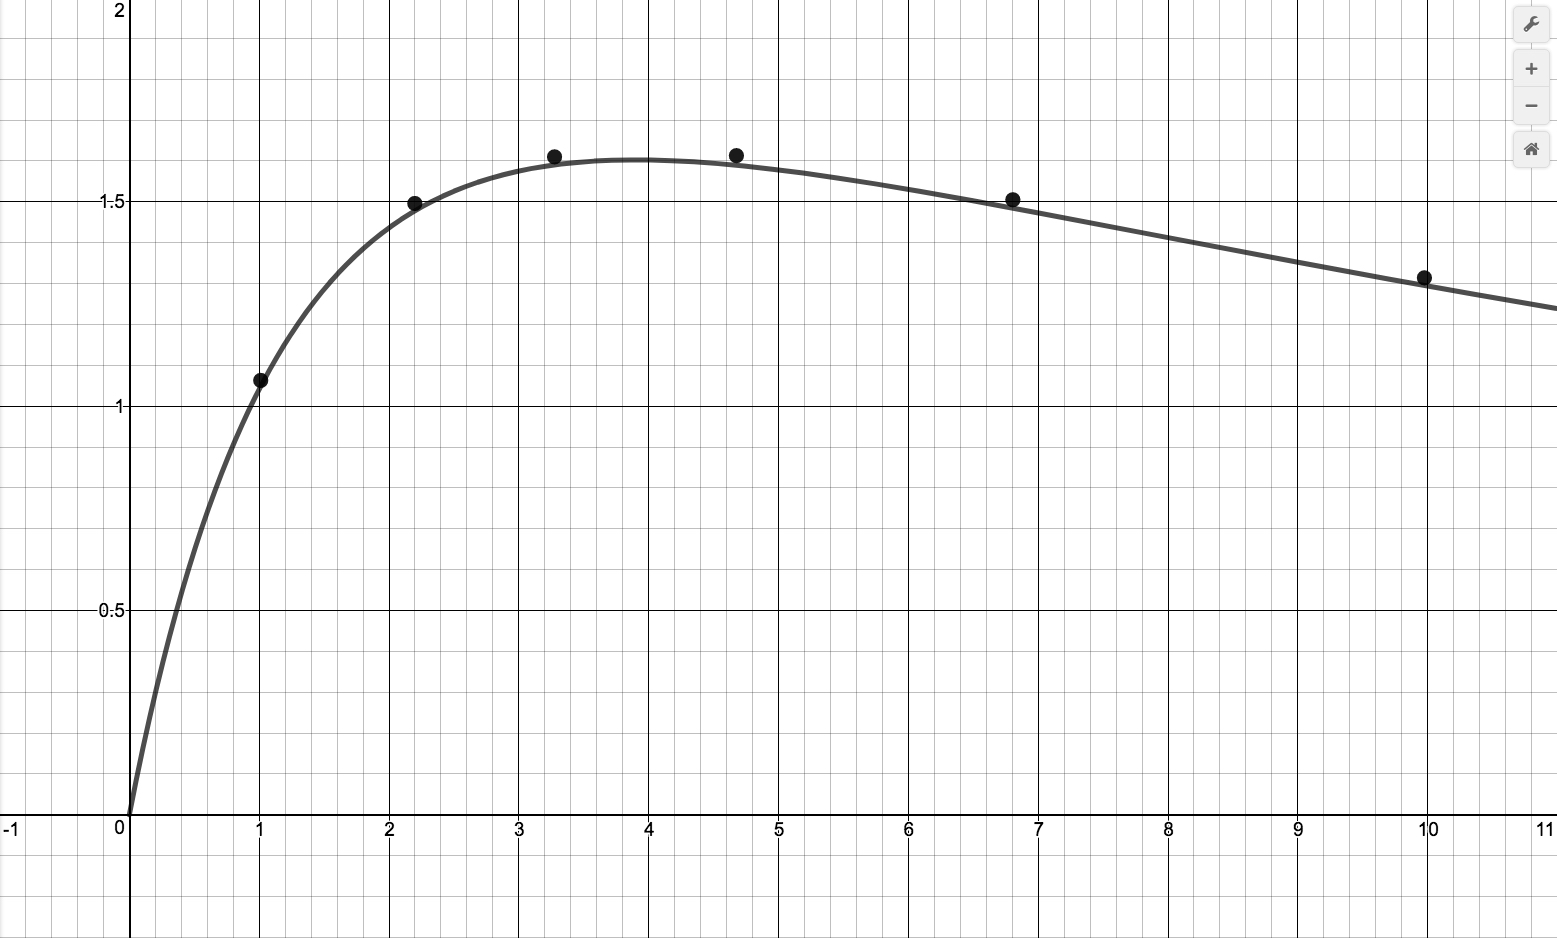
\includegraphics[height=2in]{./IntroRationalGraphics/MaxPowerRegression.jpg}

\item The maximum power is approximately $1.603 \; mW$ which corresponds to $3.9 \; k\Omega$.

\item As $x \rightarrow \infty, \; P(x) \rightarrow 0^{+}$ which means as the resistance increases without bound, the power diminishes to zero.

\end{enumerate}

\item  $a = -2$ and $c = -18$ so $f(x) = \dfrac{-2x^2+18}{x+3}$.  

\item  \begin{multicols}{2}

 \begin{enumerate}

\item   $a=6$ and $n=2$ so $f(x) = \dfrac{6x^{2} -4}{2x^2+1}$

\item  $a=10$ and $n = 3$ so $f(x) = \dfrac{10x^{3} -4}{2x^2+1}$ .

\end{enumerate}
\end{multicols}


\item  If we define $f(x) = p(x) - p(a)$ then $f$ is a polynomial function with $f(a) = p(a) - p(a) = 0$.  The Factor Theorem guarantees $(x-a)$ is a factor of $f(x)$, that is, $f(x) = p(x) - p(a) = (x-a)q(x)$ for some polynomial $q(x)$. Hence, $r(x) = \frac{p(x)-p(a)}{x-a} = \frac{(x-a)q(x)}{x-a} = q(x)$ so the graph of $y = r(x)$ is the same as the graph of the polynomial $y = q(x)$ except for a hole when $x = a$.

\item  The slope of the curves near $x=1$ matches the exponent on $x$.  This exactly what we saw in  Exercise \ref{monomialarcexercise} in Section \ref{GraphsofPolynomials}.

\[ \begin{array}{|r||c|c|c|c|}  \hline

 f(x) &  [0.9, 1.1] & [0.99, 1.01] &[0.999, 1.001] & [0.9999, 1.0001]  \\ \hline
 x^{-1} & -1.0101 & -1.0001 & \approx -1 & \approx -1  \\  \hline
 x^{-2}& -2.0406& -2.0004 & \approx -2 & \approx -2   \\  \hline
 x^{-3} &-3.1021 & -3.0010 & \approx -3 & \approx -3   \\  \hline
 x^{-4} &-4.2057 & -4.0020 &\approx -4 & \approx -4   \\   \hline


\end{array} \]

\end{enumerate}

\closegraphsfile

\newpage

\begin{comment}

\section{Graphs of Rational Functions}

\mfpicnumber{1}
\opengraphsfile{RationalGraphs}

\setcounter{footnote}{0}

\label{RationalGraphs}

In Section \ref{IntroRational}, we learned about the types of behaviors to expect from graphs of rational functions: vertical asymptotes, holes in graph, horizontal and slant asymptotes.   Moreover,  Theorems \ref{vavshole}, \ref{hathm} and \ref{sathm} tell us exactly when and where these behaviors will occur.  We used graphing technology extensively in the last section to help us verify results. In this section, we delve more deeply into graphing rational functions with the goal of sketching relatively accurate graphs without the aid of a graphing utility.  Your instructor will ultimately communicate the level of detail expected out of you when it comes to producing graphs of rational functions;  what we provide here is an attempt to glean as much information about the graph as possible given the analytical tools at our disposal.  

  \smallskip

One of the standard tools we will use is the sign diagram which was first introduced in Section \ref{QuadraticFunctions}, and then revisited in Section \ref{RealZeros}. In these sections,  to construct a sign diagram for a function $f$, we first found the zeros of $f$.  The zeros broke  the domain of $f$ into a series of intervals.  We determined the sign of $f(x)$ over the \textit{entire} interval by finding the sign of $f(x)$ for just \textit{one} test value per interval.  The theorem that justified this approach was the Intermediate Value Theorem, Theorem \ref{IVT}, which says that \textit{continuous} functions cannot change their sign between two values unless there is a zero  between those two values. 

This strategy fails in  general with rational functions.  Indeed, the very first  function we studied in Section \ref{IntroRational}, $r(x) = \frac{1}{x}$ changes sign between $x=-1$ and $x=1$, but there is no zero between these two values - instead, the graph changes sign across a vertical asymptote.  We could also well imagine the graph of a rational function having a hole where an $x$-intercept should be\footnote{Take $f(x) = \frac{x^2}{x}$, for instance.}  It turns out that with Calculus we can show rational functions are continuous on their domains.  What this means for us is when we construct sign diagrams, we need to choose test values on either side of values excluded from the domain in addition to checking around zeros.\footnote{Since excluded values are zeros of the denominator, we can think of this as really just generalizing what we already do.}


\phantomsection
\label{rationalsigndiagram}

\colorbox{ResultColor}{\bbm

\centerline{\textbf{Steps for Constructing a Sign Diagram for a  Rational Function}} 

\medskip

\hspace{.17in} Suppose $f$ is a rational function. \index{sign diagram ! rational function}

\begin{enumerate}

\item  Place any values excluded from the domain of  $f$ on the number line with an `\textinterrobang' above them.\footnote{ `\textinterrobang' is a nonstandard symbol called the \href{http://en.wikipedia.org/wiki/Interrobang}{\underline{interrobang}}.  \index{interrobang} We use this symbol to convey a sense of surprise, caution and wonderment - an appropriate attitude to take when approaching these points.}   

\item  Find the zeros of $f$ and place them on the number line with the number $0$ above them.

\item  Choose a test value in each of the intervals determined in steps 1 and 2.

\item  Determine and record the sign of $f(x)$ for each test value in step 3.

\end{enumerate}

\ebm}

\medskip 

We now present our procedure for graphing rational functions and apply it to a few exhaustive examples.  Please note that we decrease the amount of detail given in the explanations as we move through the examples.  The reader should be able to fill in any details in those steps which we have abbreviated.

\medskip

\colorbox{ResultColor}{\bbm

\centerline{\textbf{Steps for Graphing Rational Functions}}

\medskip

\hspace{.17in} Suppose $r$ is a rational function. \index{graph ! rational function}

\begin{enumerate}

\item  Find the domain of $r$.

\item  Reduce $r(x)$ to lowest terms, if applicable.

\item  Determine the location of any vertical asymptotes or holes in the graph, if they exist. 

\item  Find the axis intercepts, if they exist.

\item  Analyze the end behavior of $r$.  Find the horizontal or slant asymptote, if one exists.

\item  Use a sign diagram and plot additional points, as needed, to sketch the graph.\footnote{It doesn't hurt to check for symmetry at this point, if convenient.}

\end{enumerate}

\ebm}

\bigskip

\begin{ex}  Sketch a detailed graph of $f(x) = \dfrac{3x}{x^2-4}$.

\smallskip

{\bf Solution.}  We follow the six step procedure outlined above.

\begin{enumerate}

\item  To find the domain, we first find the excluded values.  To that end, we solve  $x^2 - 4 = 0$ and find $x = \pm 2$. Our domain is $\{ x \in \mathbb{R} \, | \,  x \neq \pm 2\}$, or, using interval notation,  $(-\infty, -2) \cup (-2,2) \cup (2,\infty)$.

\item  We check if  $f(x)$ is in lowest terms by factoring: $f(x) = \frac{3x}{(x-2)(x+2)}$.  There are no common factors which means $f(x)$ is already in lowest terms.

\item  Per Theorem \ref{vavshole}, vertical asymptotes and holes in the graph come from values excluded from the domain of $f$.  The two numbers excluded from the domain of $f$ are $x = -2$ and $x=2$ and since  $f(x)$ didn't reduce,  Theorem \ref{vavshole} tells us $x=-2$ and $x=2$ are vertical asymptotes of the graph.  We can actually go a step further at this point and determine exactly how the graph approaches the asymptote near each of these values. Though not absolutely necessary,\footnote{The sign diagram in step 6 will also determine the behavior near the vertical asymptotes.} it is good practice for those heading off to Calculus.  For the discussion that follows,  we use the factored form of $f(x) = \frac{3x}{(x-2)(x+2)}$.

\begin{itemize}

\item  \textit{The behavior of $y=f(x)$ as $x \rightarrow -2$:}  Suppose $x \rightarrow -2^{-}$.  If we were to build a table of values, we'd use $x$-values a little less than $-2$, say $-2.1$, $-2.01$ and $-2.001$.  While there is no harm in actually building a table like we did in Section \ref{IntroRational}, we want to develop a `number sense' here.  Let's think about each factor in the formula of $f(x)$ as we imagine substituting a number like $x=-2.000001$ into $f(x)$. The quantity $3x$ would be very close to $-6$, the quantity $(x-2)$ would be very close to $-4$, and the factor $(x+2)$ would be very close to $0$.  More specifically, $(x+2)$ would be a little less than $0$, in this case, $-0.000001.$  We will call such a number a `very small $(-)$', `very small' meaning close to zero in absolute value. So, mentally, as $x \rightarrow -2^{-}$, \[ f(x)   = \dfrac{3x}{(x-2)(x+2)} \approx \dfrac{-6}{(-4)\left( \text{very small $(-)$}\right)} = \dfrac{3}{2 \left( \text{very small $(-)$}\right)} \]  Now, the closer $x$ gets to $-2$, the smaller $(x+2)$ will become, so even though we are multiplying our `very small $(-)$' by $2$, the denominator will continue to get smaller and smaller, and remain negative.  The result is a fraction whose numerator is positive, but whose denominator is very small and negative.  Mentally, \[f(x) \approx \dfrac{3}{2 \left( \text{very small $(-)$}\right)} \approx \dfrac{3}{\text{very small $(-)$}} \approx \text{very big $(-)$}\]  The term `very big $(-)$' means a number with a large absolute value which is negative.\footnote{The actual retail value of $f(-2.000001)$ is approximately $-1,\!500,\!000$.}  What all of this means is that as $x \rightarrow -2^{-}$, $f(x) \rightarrow -\infty$.  Now suppose we wanted to determine the behavior of $f(x)$ as $x \rightarrow -2^{+}$.  If we imagine substituting something a little larger than $-2$ in for $x$, say $-1.999999$, we mentally estimate \[ f(x) \approx \dfrac{-6}{(-4)\left( \text{very small $(+)$}\right)} = \dfrac{3}{2 \left( \text{very small $(+)$}\right)}  \approx \dfrac{3}{\text{very small $(+)$}} \approx \text{very big $(+)$}\]  We conclude that as $x \rightarrow -2^{+}$, $f(x) \rightarrow \infty$.

\item  \textit{The behavior of $y=f(x)$ as $x \rightarrow 2$:} Consider $x \rightarrow 2^{-}$. We imagine substituting $x = 1.999999$.  Approximating $f(x)$ as we did above, we get \[ f(x) \approx \dfrac{6}{\left( \text{very small $(-)$}\right)(4)} = \dfrac{3}{2 \left( \text{very small $(-)$}\right)}  \approx \dfrac{3}{\text{very small $(-)$}} \approx \text{very big $(-)$}\]  We conclude that as $x \rightarrow 2^{-}$, $f(x) \rightarrow -\infty$.  Similarly, as $x \rightarrow 2^{+}$, we imagine substituting $x = 2.000001$ to get $f(x) \approx \frac{3}{\text{\scriptsize very small $(+)$}} \approx \text{very big (+)}$.  So as $x \rightarrow 2^{+}, f(x) \rightarrow \infty$.
\end{itemize}

We interpret this graphically below on the left.


\item  To find the $x$-intercepts of the graph, we set $y=f(x) = 0$.  Solving $ \frac{3x}{(x-2)(x+2)} = 0$ results in $x=0$.  Since $x=0$ is in our domain, $(0,0)$ is the $x$-intercept.   This is also the $y$-intercept,\footnote{Per Exercise \ref{onlyoneyintexercise}, functions can have at most one $y$-intercept. Since $(0,0)$ is on the graph,  it is \textit{the} $y$-intercept.} as we can quickly verify since $f(0) = \frac{3(0)}{0^2-4} = 0$.


\item  Next, we determine the end behavior of the graph of $y=f(x)$.  Since the degree of the numerator is $1$, and the degree of the denominator is $2$, Theorem \ref{hathm} tells us that $y=0$ is the horizontal asymptote.  As with the vertical asymptotes, we can glean more detailed information using `number sense'. For the discussion below, we use the formula $f(x) = \frac{3x}{x^2-4}$. 

\begin{itemize}

\item  \textit{The behavior of $y=f(x)$ as $x \rightarrow -\infty$:}  If we were to make a table of values to discuss the behavior of $f$ as $x \rightarrow -\infty$, we would substitute very `large' negative numbers in for $x$, say for example, $x = \text{$-1$ billion}$.  The numerator $3x$ would then be $-3 \, \text{billion}$, whereas the denominator $x^2-4$ would be $(\text{$-1$ billion})^2 - 4$, which is pretty much the same as  $1(\text{billion})^2$.  Hence, \[f\left(\text{$-1$ billion}\right) \approx \dfrac{-3 \, \text{billion}}{1(\text{billion})^2} \approx - \dfrac{3}{\text{billion}} \approx \text{very small $(-)$} \]

Notice that if we substituted in $x = \text{$-1$ trillion}$, essentially the same kind of cancellation would happen, and we would be left with an even `smaller' negative number.  This not only confirms the fact that as $x \rightarrow -\infty$, $f(x) \rightarrow 0$, it tells us that $f(x) \rightarrow 0^{-}$. In other words, the graph of $y=f(x)$ is a little bit \textit{below} the $x$-axis as we move to the far left.


\item  \textit{The behavior of $y=f(x)$ as $x \rightarrow \infty$:}  On the flip side, we can imagine substituting very large positive numbers in for $x$ and looking at the behavior of $f(x)$.   For example, let $x = \text{$1$ billion}$. Proceeding as before, we get \[f\left(\text{$1$ billion}\right) \approx \dfrac{3 \, \text{billion}}{1(\text{billion})^2} \approx \dfrac{3}{\text{billion}} \approx \text{very small $(+)$} \]  The larger the number we put in, the smaller the positive number we would get out.  In other words, as $x \rightarrow \infty$, $f(x) \rightarrow 0^{+}$, so the graph of $y=f(x)$ is a little bit \emph{above} the $x$-axis as we look toward the far right.  

\end{itemize}

We interpret these findings graphically below on the right.

\begin{center}

\begin{tabular}{cc}

\begin{mfpic}[15]{-4}{4}{-5}{5}

\dashed \polyline{(-2,-4.5), (-2,4.5)}
\dashed \polyline{(2,-4.5), (2,4.5)}
\tlabel[cc](4,-0.5){\scriptsize $x$}
\tlabel[cc](0.5,5){\scriptsize $y$}
\axes
\xmarks{-3 step 1 until 3}
\tiny
\tlpointsep{4pt}
\axislabels {x}{ {$-3\hspace{7pt}$} -3, {$-1\hspace{7pt}$} -1,  {$1$} 1, {$3$} 3}
\normalsize
\penwd{1.25pt}
\arrow \curve{(-2.75,-3),(-2.5,-3.25), (-2.25,-4)}
\arrow \reverse \curve{(-1.75,4),(-1.5,3.25), (-1.25,3)}
\arrow \curve{(1.25,-3), (1.5,-3.25) , (1.75,-4)}
\arrow \curve{(2.75,3),(2.5,3.25), (2.25,4)}
\end{mfpic}

&

\begin{mfpic}[15]{-4.75}{4.75}{-2}{2}
\tlabel[cc](4.75,-0.5){\scriptsize $x$}
\tlabel[cc](0.5,2){\scriptsize $y$}
\axes
\ymarks{-1 step 1 until 1}
\tiny
\tlpointsep{4pt}
\axislabels {y}{{$-1$} -1, {$1$} 1}
\normalsize
\penwd{1.25pt}
\arrow \curve{(2.5,0.85), (3,0.35), (4.25, 0.15)}
\arrow \curve{(-2.5,-0.85), (-3,-0.35), (-4.25, -0.15)}
\end{mfpic} \\

behavior near $x = \pm 2$  & end behavior

\end{tabular}

\end{center}

\item  Lastly, we construct a sign diagram for $f(x)$.  The $x$-values excluded from the domain of $f$ are $x = \pm 2$, and the only zero of $f$ is $x=0$.  Displaying these appropriately on the number line gives us four test intervals, and we choose the test values\footnote{In this particular case, we don't need test values since our analysis of the behavior of $f$ near the vertical asymptotes and our end behavior analysis have given us the signs on each of the test intervals.  In general, however, this won't always be the case, so for demonstration purposes, we continue with our usual construction.} $x=-3$, $x=-1$, $x=1$ and $x=3$.  We find $f(-3)$ is $(-)$, $f(-1)$ is $(+)$, $f(1)$ is $(-)$ and $f(3)$ is $(+)$.  As we begin our sketch, it certainly appears as if the graph could be symmetric about the origin.  Taking a moment to check for symmetry, we find $f(-x) = \frac{3(-x)}{(-x)^2-4} = -\frac{3x}{x^2-4} = -f(x)$.  Hence, $f$ is odd and the graph of $y = f(x)$ is symmetric about the origin. Putting all of our work together, we get the graph below.

\begin{tabular}{m{0.5in}m{2in}m{2.5in}}

&

\begin{mfpic}[10]{-6}{6}{-2}{2}
\arrow \reverse \arrow \polyline{(-6,0),(6,0)}
\xmarks{-3,0,3}
\arrow \polyline{(-4.5,-1.5),(-4.5,-0.5)}
\arrow \polyline{(-1.5,-1.5),(-1.5,-0.5)}
\arrow \polyline{(1.5,-1.5),(1.5,-0.5)}
\arrow \polyline{(4.5,-1.5),(4.5,-0.5)}
\tlpointsep{4pt}
\axislabels {x}{{$-2$} -3, {$0$} 0, {$2$} 3 }
\tlabel[cc](-4.5,1){$(-)$}
\tlabel[cc](-4.5,-2.25){$-3$}
\tlabel[cc](-3,1){\textinterrobang}
\tlabel[cc](-1.5,1){$(+)$}
\tlabel[cc](-1.75,-2.25){$-1$}
\tlabel[cc](0,1){$0$}
\tlabel[cc](1.5,1){$(-)$}
\tlabel[cc](1.5,-2.25){$1$}
\tlabel[cc](3,1){\textinterrobang}
\tlabel[cc](4.5,1){$(+)$}
\tlabel[cc](4.5,-2.25){$3$}
\end{mfpic} 

&

\begin{mfpic}[16]{-6}{6}{-4}{4}

\dashed \polyline{(-2,-4), (-2,4)}
\dashed \polyline{(2,-4), (2,4)}
\tlabel[cc](6,-0.5){\scriptsize $x$}
\tlabel[cc](0.5,4){\scriptsize $y$}
\axes
\xmarks{-5 step 1 until 5}
\ymarks{-3 step 1 until 3}
\tiny
\tlpointsep{4pt}
 \axislabels {x}{ {$-5\hspace{7pt}$} -5, {$-4 \hspace{7pt}$} -4 ,{$-3\hspace{7pt}$} -3, {$-1\hspace{7pt}$} -1,  {$1$} 1, {$3$} 3,  {$4$} 4, {$5$} 5}
\axislabels {y}{ {$-3$} -3, {$-2$} -2,{$-1$} -1, {$1$} 1, {$2$} 2,{$3$} 3}
\normalsize
\penwd{1.25pt}
\arrow \reverse \arrow \function{-6, -2.5, 0.1}{(3*x)/((x**2)-4)}
\arrow \reverse \arrow \function{-1.5, 1.5, 0.1}{(3*x)/((x**2)-4)}
\arrow \reverse \arrow \function{2.5, 6, 0.1}{(3*x)/((x**2)-4)}
\point[4pt]{(0,0)}
\end{mfpic}

\end{tabular}

\end{enumerate}

\qed

\end{ex}

Something important to note about the above example is that while $y=0$ is the horizontal asymptote, the graph of $f$ actually crosses the $x$-axis at $(0,0)$.  The myth that graphs of rational functions can't cross their horizontal asymptotes is completely false,\footnote{That's why we called it a MYTH!} as we shall see again in our next example.

\begin{ex}  Sketch a detailed graph of $g(t) = \dfrac{2t^2-3t-5}{t^2-t-6}$.

{\bf Solution.}

\begin{enumerate}

\item  To find the values excluded from the domain of $g$, we solve  $t^2-t-6 = 0$ and find $t = -2$ and $t=3$.  Hence, our domain is $\{ t \in \mathbb{R} \, | \, t \neq -2 3 \}$, or using interval notation: $(-\infty, -2) \cup (-2,3) \cup (3,\infty)$.

\item  To check if $g(t)$ is in lowest terms, we factor:  $g(t) = \frac{(2t-5)(t+1)}{(t-3)(t+2)}$.  There is no cancellation, so $g(t)$ is in lowest terms.

\item  Since $g(t)$ was given to us in lowest terms, we have, once again by Theorem \ref{vavshole} vertical asymptotes $t=-2$ and $t=3$.  Keeping in mind $g(t) = \frac{(2t-5)(t+1)}{(t-3)(t+2)}$, we proceed to our analysis near each of these values.

\begin{itemize}

\item  \textit{The behavior of $y=g(t)$ as $t \rightarrow -2$:}  As $t \rightarrow -2^{-}$, we imagine substituting a number a little bit less than $-2$. We have \[g(t) \approx \frac{(-9)(-1)}{(-5)(\text{very small $(-)$})} \approx \frac{9}{\text{very small $(+)$}} \approx \text{very big (+)}\] so as $t \rightarrow -2^{-}$, $g(t) \rightarrow \infty$. On the flip side, as $t \rightarrow -2^{+}$, we get \[g(t) \approx \frac{9}{\text{ very small $(-)$}} \approx \text{very big $(-)$}\] so $g(t) \rightarrow -\infty$.

\item  \textit{The behavior of $y=g(t)$ as $x \rightarrow 3$:}  As $t \rightarrow 3^{-}$, we imagine plugging in a number just shy  of $3$. We have \[g(t) \approx \frac{(1)(4)}{(\text{ very small $(-)$}) (5)} \approx \frac{4}{\text{very small $(-)$}} \approx \text{very big $(-)$}\] Hence, as $t \rightarrow 3^{-}$, $g(t) \rightarrow -\infty$. As $t \rightarrow 3^{+}$, we get \[g(t) \approx \frac{4}{\text{ very small $(+)$}} \approx \text{very big $(+)$}\] so $g(x) \rightarrow \infty$.

\end{itemize}

We interpret this analysis graphically below on the left.


\item  To find the $t$-intercepts  we set $y = g(t) = 0$.  Using the factored form of $g(t)$ above, we find the zeros to be the solutions of $(2t-5)(t+1)=0$.  We obtain $t = \frac{5}{2}$ and $t=-1$. Since both of these numbers are in the domain of $g$, we have two $t$-intercepts, $\left( \frac{5}{2},0\right)$ and $(-1,0)$.  To find the $y$-intercept, we find $y = g(0) = \frac{5}{6}$, so our $y$-intercept is $\left(0, \frac{5}{6}\right)$.

\item  Since the degrees of the numerator and denominator of $g(t)$ are the same, we know from Theorem \ref{hathm} that we can find the horizontal asymptote of the graph of $g$ by taking the ratio of the leading terms coefficients, $y = \frac{2}{1} = 2$.  However, if we take the time to do a more detailed analysis, we will be able to reveal some `hidden' behavior which would be lost otherwise.  Using long division, we may rewrite $g(t)$ as $g(t) = 2 - \frac{t-7}{t^2-t-6}.$  We focus our attention on the term $\frac{t-7}{t^2-t-6}$.  

\begin{itemize}

\item  \textit{The behavior of $y=g(t)$ as $t \rightarrow -\infty$:} If imagine substituting $t = \text{$-1$ billion}$ into $\frac{t-7}{t^2-t-6}$, we estimate $\frac{t-7}{t^2-t-6} \approx \frac{\text{\scriptsize $-1$ billion}}{1 \text{\scriptsize billion}^2}  = \frac{-1}{\text{\scriptsize billion}} \approx \text{very small $(-)$}$.\footnote{We are once again using the fact that for polynomials, end behavior is determined by the leading term, so in the denominator, the $t^2$ term dominates the $t$ and constant terms.}  Hence, \[g(t) =  2 - \frac{t-7}{t^2-t-6} \approx 2 - \text{very small $(-)$} = 2 + \text{very small $(+)$}\]  Hence, as $t \rightarrow -\infty$, the graph is a little bit \textit{above} the line $y=2$.

\item  \textit{The behavior of $y=g(t)$ as $t \rightarrow \infty$.}  To consider $\frac{t-7}{t^2-t-6}$ as $t \rightarrow \infty$, we imagine substituting $t= \text{$1$ billion}$ and, going through the usual mental routine, find \[\frac{t-7}{t^2-t-6} \approx \text{very small $(+)$}\]  Hence, $g(t) \approx 2 - \ \text{very small $(+)$}$, so the graph is just \textit{below} the line $y=2$ as $t \rightarrow \infty$.

\end{itemize}

We sketch the end behavior below on the right.




\begin{center}

\begin{tabular}{cc}

\begin{mfpic}[15]{-5}{5}{-5}{5}
\dashed \polyline{(-2,-4.5), (-2,4.5)}
\dashed \polyline{(3,-4.5), (3,4.5)}
\tlabel[cc](5,-0.5){\scriptsize $t$}
\tlabel[cc](0.5,5){\scriptsize $y$}
\axes
\xmarks{-4 step 1 until 4}
\tiny
\tlpointsep{4pt}
\axislabels {x}{ {$-3\hspace{7pt}$} -3, {$-1\hspace{7pt}$} -1,  {$1$} 1, {$2$} 2, {$4$} 4}
\normalsize
\penwd{1.25pt}
\arrow \curve{(-2.75,3),(-2.5,3.25), (-2.25,4)}
\arrow \reverse \curve{(-1.75,-4),(-1.5,-3.25), (-1.25,-3)}
\arrow \curve{(2.25,-3), (2.5,-3.25) , (2.75,-4)}
\arrow \curve{(3.75,3),(3.5,3.25), (3.25,4)}
\end{mfpic}

&

\begin{mfpic}[15]{-4.75}{4.75}{-1}{3}
\dashed \polyline{(-4.75,2), (4.75,2)}
\tlabel[cc](4.75,-0.5){\scriptsize $t$}
\tlabel[cc](0.5,3){\scriptsize $y$}
\axes
\ymarks{-1 step 1 until 1}
\tiny
\tlpointsep{4pt}
\axislabels {y}{{$-1$} -1, {$1$} 1}
\normalsize
\penwd{1.25pt}
\arrow \curve{(2.5,1.15), (3,1.65), (4.25, 1.85)}
\arrow \curve{(-2.5,2.85), (-3,2.35), (-4.25, 2.15)}
\end{mfpic} \\

behavior near $t = -2$ and $t = 3$ & end behavior \\

\end{tabular}

\end{center}

\item  Finally we construct our sign diagram.  We place an `\textinterrobang' above $t=-2$ and $t=3$, and a `$0$' above $t = \frac{5}{2}$ and $t=-1$.  Choosing test values in the test intervals gives us $g(t)$ is $(+)$ on the intervals $(-\infty, -2)$, $\left(-1, \frac{5}{2}\right)$ and $(3, \infty)$, and $(-)$ on the intervals $(-2,-1)$ and $\left(\frac{5}{2}, 3\right)$.  As we piece together all of the information, it stands to reason the graph must cross the horizontal asymptote at some point after $t=3$ in order for it to approach $y=2$ from underneath.\footnote{This subtlety would have been missed had we skipped the long division and subsequent end behavior analysis.}   To find where $y = g(t)$ intersects $y = 2$, we solve $g(t) =  2 - \frac{t-7}{t^2-t-6} = 2$ and get $t-7= 0$, or $t=7$.  Note that $t-7$ is the remainder when $2t^2-3t-5$ is divided by $t^2-t-6$, so it makes sense that for $g(t)$ to equal the quotient $2$, the remainder from the division must be $0$.  Sure enough, we find $g(7)=2$.  The location of the $t$-intercepts alone dashes all hope of the function being even or odd (do you see why?) so we skip the symmetry check in this case.

\begin{tabular}{m{0.05in}m{2.5in}m{2.5in}}

&

\begin{mfpic}[10]{-8}{7}{-2}{2}
\arrow \reverse \arrow \polyline{(-8,0),(7,0)}
\xmarks{-5,-2,1,4}
\tlpointsep{4pt}
\axislabels {x}{{$-2$} -5, {$-1$} -2, {$\frac{5}{2}$} 1, {$3$} 4}
\tlabel[cc](-6.5,1){$(+)$}
\tlabel[cc](-5,1){\textinterrobang}
\tlabel[cc](-3.5,1){$(-)$}
\tlabel[cc](-2,1){$0$}
\tlabel[cc](-0.5,1){$(+)$}
\tlabel[cc](1,1){$0$}
\tlabel[cc](2.5,1){$(-)$}
\tlabel[cc](4,1){\textinterrobang}
\tlabel[cc](5.5,1){$(+)$}
\end{mfpic}

& 

\begin{mfpic}[10]{-10}{10}{-5}{9}

\dashed \polyline{(-2,-5), (-2,9)}
\dashed \polyline{(3,-5), (3,9)}
\dashed \polyline{(-10,2), (10,2)}
\tlabel[cc](10,-0.5){\scriptsize $t$}
\tlabel[cc](0.5,9){\scriptsize $y$}
\axes
\xmarks{-9 step 1 until 9}
\ymarks{-4 step 1 until 8}
\tiny
\tlpointsep{4pt}
\axislabels {x}{ {$-9\hspace{7pt}$} -9, {$-8 \hspace{7pt}$} -8 ,{$-7 \hspace{7pt}$} -7, {$-6 \hspace{7pt}$} -6,{$-5\hspace{7pt}$} -5, {$-4 \hspace{7pt}$} -4 ,{$-3\hspace{7pt}$} -3, {$-1\hspace{7pt}$} -1,  {$1$} 1, {$2$} 2,  {$4$} 4, {$5$} 5, {$6$} 6,  {$7$} 7, {$8$} 8, {$9$} 9}
\axislabels {y}{ {$-4$} -4,{$-3$} -3, {$-2$} -2,{$-1$} -1, {$1$} 1, {$3$} 3, {$4$} 4, {$5$} 5, {$6$} 6, {$7$} 7, {$8$} 8}
\normalsize
\penwd{1.25pt}
\arrow \reverse \arrow \function{-9, -2.29, 0.1}{(2*(x**2)-3*x-5)/((x**2)-x-6)}
\arrow \reverse \arrow \function{-1.69, 2.86, 0.1}{(2*(x**2)-3*x-5)/((x**2)-x-6)}
\arrow \reverse \arrow \function{3.12, 9, 0.1}{(2*(x**2)-3*x-5)/((x**2)-x-6)}
\point[4pt]{(-1,0), (2.5,0), (0, 0.83333)}
\end{mfpic}

\end{tabular}

\end{enumerate}

\qed

\end{ex}

More can be said about the graph of $y = g(t)$ above.   It stands to reason that $g$ must attain a local  minimum at some point past $t=7$ since the graph of $g$ crosses through $y=2$  at $(2,7)$ but approaches $y=2$ from below as $t \rightarrow \infty$.  Calculus verifies a local minimum at $(13, 1.96)$.  We invite the reader to verify this claim using a graphing utility. 

\begin{ex}  Sketch a detailed graph of $h(x) = \dfrac{2x^3+5x^2+4x+1}{x^2+3x+2}$.

{ \bf Solution.}  

\begin{enumerate}

\item   Solving $x^2+3x+2 = 0$ gives $x = -2$ and $x=-1$ as our excluded values.  Hence, the domain is $\{ x \in \mathbb{R} \, | \, x \neq -1, -2 \}$ or, using interval notation,  $(-\infty, -2) \cup (-2, -1) \cup (-1, \infty)$.

\item  To reduce $h(x)$, we need to factor the numerator and denominator.  To factor the numerator, we use the techniques\footnote{Bet you never thought you'd never see \textit{that} stuff again before the Final Exam!} set forth in Section \ref{RealZeros} and get  \[h(x) =  \dfrac{2x^3+5x^2+4x+1}{x^2+3x+2} = \dfrac{(2x+1)(x+1)^2}{(x+2)(x+1)} = \dfrac{ (2x+1) (x+1)^{\cancelto{1}{2}}  }{(x+2)\cancel{(x+1)}} = \dfrac{(2x+1)(x+1)}{x+2} \]

Note we can use this formula for $h(x)$ in our analysis of the graph of $h$ as long as we are not substituting $x=-1$.  To make this exclusion specific, we write $h(x) = \frac{(2x+1)(x+1)}{x+2}$, $x \neq -1$.

\item  From Theorem \ref{vavshole}, we know that since $x=-2$ is a zero of the denominator of the reduced form of $h(x)$, we have a vertical asymptote there.  As for $x=-1$, the factor $(x+1)$ was canceled from the denominator when we reduced $h(x)$, so there will be a hole when $x=-1$.  To find the $y$-coordinate of the hole, we substitute $x=-1$ into $\frac{(2x+1)(x+1)}{x+2}$, per Theorem \ref{vavshole} and get $0$.  Hence, we have a hole on the $x$-axis at $(-1,0)$.  It should make you uncomfortable plugging $x=-1$ into the reduced formula for $h(x)$, especially since we've made such a big deal about the stipulation  `$x \neq -1$' that goes along with that formula.  What we are really doing is taking a Calculus short-cut to the more detailed kind of analysis near $x=-1$ which we will show below. 
\begin{itemize}

\item  \textit{The behavior of $y=h(x)$ as $x \rightarrow -2$:}  As $x \rightarrow -2^{-}$, we imagine substituting a number a little bit less than $-2$. We have $h(x) \approx \frac{(-3)(-1)}{(\text{\scriptsize very small $(-)$})} \approx \frac{3}{(\text{\scriptsize very small $(-)$})}\approx \text{very big $(-)$}$ thus as $x \rightarrow -2^{-}$, $h(x) \rightarrow -\infty$. On the other side of $-2$, as $x \rightarrow -2^{+}$, we find that $h(x) \approx \frac{3}{\text{\scriptsize very small $(+)$}} \approx \text{very big $(+)$}$, so $h(x) \rightarrow \infty$.

\item  \textit{The behavior of $y=h(x)$ as $x \rightarrow -1$.}  As $x \rightarrow -1^{-}$, we imagine plugging in a number a bit less than $x=-1$. We have $h(x) \approx \frac{(-1)(\text{\scriptsize very small $(-)$})}{1} = \text{very small $(+)$}$ Hence, as $x \rightarrow -1^{-}$, $h(x) \rightarrow 0^{+}$. This means that as $x \rightarrow -1^{-}$, the graph is a bit above the point $(-1,0)$.  As $x \rightarrow -1^{+}$, we get $h(x) \approx \frac{(-1)(\text{\scriptsize very small $(+)$})}{1} = \text{very small $(-)$}$.  This gives us that as $x \rightarrow -1^{+}$, $h(x) \rightarrow 0^{-}$, so the graph is a little bit lower than $(-1,0)$ here.  

\end{itemize}

We interpret this graphically below on the left.

\item  To find the $x$-intercepts, as usual, we set $h(x) = 0$ and solve.  Solving $\frac{(2x+1)(x+1)}{x+2}=0$ yields $x=-\frac{1}{2}$ and $x=-1$.  The latter isn't in the domain of $h$, in fact, we know there is a hole at $(-1,0)$,  so we exclude it.  Our only $x$-intercept is $\left(-\frac{1}{2}, 0\right)$.  To find the $y$-intercept, we set $x=0$.  Since $0 \neq -1$, we can use the reduced formula for $h(x)$ and we get $h(0) = \frac{1}{2}$ for a $y$-intercept of $\left(0,\frac{1}{2}\right)$.


\item  For end behavior, we note that the degree of the numerator of $h(x)$, $2x^3+5x^2+4x+1$, is $3$ and the degree of the denominator, $x^2+3x+2$, is $2$ so by Theorem \ref{sathm}, the graph of $y = h(x)$ has a slant asymptote.  For $x\rightarrow \pm \infty$, we are far enough away from $x=-1$ to use the reduced formula, $h(x) = \frac{(2x+1)(x+1)}{x+2}$, $x \neq -1$.  To perform long division, we multiply out the numerator and get $h(x) = \frac{2x^2+3x+1}{x+2}$, $x \neq -1$, and rewrite $h(x) = 2x-1+\frac{3}{x+2}$, $x \neq -1$.  By Theorem \ref{sathm}, the slant asymptote is $y = 2x-1$, and to better see \textit{how} the graph approaches the asymptote, we focus our attention on the term generated from the remainder, $\frac{3}{x+2}$.

\begin{itemize}

\item  \textit{The behavior of $y=h(x)$ as $x \rightarrow -\infty$:} Substituting  $x = \text{$-1$ billion}$ into $\frac{3}{x+2}$, we get the estimate $\frac{3}{\text{\scriptsize $-1$ billion}} \approx \text{very small $(-)$}$.  Hence, $h(x) = 2x-1+\frac{3}{x+2} \approx 2x-1 + \text{very small $(-)$}$.  This means the graph of $y=h(x)$ is a little bit \textit{below} the line $y=2x-1$ as $x \rightarrow -\infty$.

\item  \textit{The behavior of $y=h(x)$ as $x \rightarrow \infty$:}  If $x \rightarrow \infty$, then $\frac{3}{x+2} \approx \text{very small $(+)$}$.  This means $h(x) \approx 2x-1 + \text{very small $(+)$}$, or that the graph of $y=h(x)$ is a little bit \textit{above} the line $y=2x-1$ as $x \rightarrow \infty$.

\end{itemize}

We sketch the end behavior below on the right.
 
 \begin{center}
 
 \begin{tabular}{cc}

\begin{mfpic}[15]{-4}{1}{-5}{5}

\dashed \polyline{(-2,-4.5), (-2,4.5)}
\tlabel[cc](1,-0.5){\scriptsize $x$}
\tlabel[cc](0.5,5){\scriptsize $y$}
\axes
\xmarks{-2,-1}
\tiny
\tlpointsep{4pt}
\axislabels {x}{ {$-3\hspace{7pt}$} -3}
\normalsize
\penwd{1.25pt}
\arrow \curve{(-2.75,-3),(-2.5,-3.25), (-2.25,-4)}
\arrow \reverse \curve{(-1.75,4),(-1.5,3.25), (-1.25,3)}
\curve{(-1.25,0.5), (-1,0), (-0.75,-0.5)}
\pointfillfalse
\point[4pt]{(-1,0)}
\end{mfpic}

&

\begin{mfpic}[15]{-4.75}{4.75}{-4.75}{4.75}

\dashed \function{-1.7,2.7,0.1}{2*x-1}
\tlabel[cc](4.75,-0.5){\scriptsize $x$}
\tlabel[cc](0.5,4.75){\scriptsize $y$}
\axes
\ymarks{-4 step 4 until 1}
\tiny
\tlpointsep{4pt}
\axislabels {y}{{$-4$} -4,{$-3$} -3,{$-2$} -2,{$-1$} -1, {$1$} 1, {$2$} 2, {$3$} 3, {$4$} 4}
\normalsize
\penwd{1.25pt}
\arrow \curve{(-1.25,-4), (-1.5,-4.2), (-1.7, -4.75)}
\arrow \curve{(2.25,4), (2.5,4.2), (2.75, 4.75)}
\end{mfpic} \\

behavior near $x = -2$ and $x=-1$ & end behavior

\end{tabular}

\end{center}

\item  To make our sign diagram, we place an `\textinterrobang' above $x=-2$ and $x=-1$ and a `$0$' above $x=-\frac{1}{2}$.  On our four test intervals, we find $h(x)$ is $(+)$ on $(-2,-1)$ and $\left(-\frac{1}{2}, \infty\right)$ and $h(x)$ is $(-)$ on $(-\infty, -2)$ and $\left(-1,-\frac{1}{2}\right)$.  Putting all of our work together yields the graph below.

\end{enumerate}

\begin{tabular}{m{0.5in}m{2in}m{2.5in}}

&

\begin{mfpic}[10]{-8}{8}{-2}{2}
\arrow \reverse \arrow \polyline{(-8,0),(8,0)}
\xmarks{-4,0,4}
\tlpointsep{6pt}
\axislabels {x}{{$-2 \hspace{9pt}$} -4, {$-1 \hspace{9pt}$} 0, {$-\frac{1}{2} \hspace{9pt}$} 4}
\tlabel[cc](-6,1){$(-)$}
\tlabel[cc](-4,1){\textinterrobang}
\tlabel[cc](-2.25,1){$(+)$}
\tlabel[cc](0,1){\textinterrobang}
\tlabel[cc](2.25,1){$(-)$}
\tlabel[cc](4,1){$0$}
\tlabel[cc](6,1){$(+)$}
\end{mfpic} 

&

\begin{mfpic}[16][8]{-5}{5}{-15}{10}

\dashed \polyline{(-2,-15), (-2,10)}
\dashed \function{-7,5.5,0.1}{2*x-1}
\tlabel[cc](5,-0.5){\scriptsize $x$}
\tlabel[cc](0.5,10){\scriptsize $y$}
\axes
\xmarks{-4 step 1 until 4}
\ymarks{-14 step 1 until 9}
\tiny
\tlpointsep{4pt}
\axislabels {x}{{$-4 \hspace{7pt}$} -4 ,{$-3\hspace{7pt}$} -3, {$-1\hspace{7pt}$} -1,  {$1$} 1,{$2$} 2, {$3$} 3,  {$4$} 4}
\axislabels {y}{ {$-14$} -14, {$-13$} -13,{$-12$} -12,{$-11$} -11, {$-10$} -10,{$-9$} -9,{$-8$} -8, {$-7$} -7,{$-6$} -6,{$-5$} -5, {$-4$} -4,{$-3$} -3, {$-2$} -2,{$-1$} -1, {$1$} 1, {$2$} 2,{$3$} 3, {$4$} 4,{$5$} 5, {$6$} 6,{$7$} 7, {$8$} 8,{$9$} 9}
\normalsize
\penwd{1.25pt}
\arrow \reverse \arrow \function{-6.67, -2.32, 0.1}{(2*(x**2)+3*x+1)/(x+2)}
\arrow \reverse \arrow \function{-1.79, 5.29, 0.1}{(2*(x**2)+3*x+1)/(x+2)}
\point[4pt]{(-0.5,0)}
\pointfillfalse
\point[4pt]{(-1,0)}
\end{mfpic}

\end{tabular}

To find if the graph of $h$ ever crosses the slant asymptote, we solve $h(x) = 2x-1+\frac{3}{x+2}= 2x-1$.  This results in $\frac{3}{x+2} = 0$, which has no solution.\footnote{Alternatively, the remainder after the long division was $r=3$ which is never $0$.} Hence, the graph of $h$ never crosses its slant asymptote.\footnote{But rest assured, some graphs do!}
\qed


\end{ex}

Our last graphing example is challenging in that our six step process provides us little information to work with.

\begin{ex}   \label{carefulanalysisneeded} Sketch the graph of $r(x) = \dfrac{x^4+1}{x^2+1}$.

\smallskip

{\bf Solution.}

\begin{enumerate}

\item  The denominator $x^2+1$ is never zero which means there are no excluded values.  The domain is $\mathbb{R}$, or using interval notation,  $(-\infty, \infty)$.

\item  With no real zeros in the denominator, $x^2+1$ is an irreducible quadratic.  Our only hope of reducing $r(x)$ is if $x^2+1$ is a factor of $x^4+1$.  Performing long division gives us \[\frac{x^4+1}{x^2+1} = x^2-1+\frac{2}{x^2+1}\] The remainder is not zero so $r(x)$ is already reduced.

\item Since there are no numbers excluded from the domain of $r$, there are no vertical asymptotes or holes in the graph of $r$.

\item  To find the $x$-intercept, we'd set $r(x) = 0$.  Since there are no real solutions to $x^4+1=0$, we have no $x$-intercepts.  Since $r(0) = 1$, we do get $(0,1)$ as the $y$-intercept.

\item  For end behavior, we note that since the degree of the numerator is exactly \textit{two} more than the degree of the denominator, neither Theorems \ref{hathm} nor \ref{sathm} apply.\footnote{This won't stop us from giving it the old community college try, however!} We know from our attempt to reduce $r(x)$ that we can rewrite $r(x) = x^2-1+\frac{2}{x^2+1}$, so we focus our attention on the term corresponding to the remainder, $\frac{2}{x^2+1}$  It should be clear that as $x \rightarrow \pm \infty$, $\frac{2}{x^2+1} \approx \text{very small $(+)$}$, which means $r(x) \approx x^2-1 + \text{very small $(+)$}$.  So the graph $y=r(x)$ is a little bit \textit{above} the graph of the parabola $y=x^2-1$ as $x \rightarrow \pm \infty$. Graphically,



\item  There isn't much work to do for a sign diagram for $r(x)$, since its domain is all real numbers and it has no zeros.  Our sole test interval is $(-\infty, \infty)$, and since we know $r(0) = 1$, we conclude $r(x)$ is $(+)$ for all real numbers.   We check for symmetry, and find $r(-x) = \frac{(-x)^4+1}{(-x)^2+1} = \frac{x^4+1}{x^2+1} = r(x)$, so $r$ is even and, hence, the graph is symmetric about the $y$-axis.  It may be tempting at this point to call it quits, reach for a graphing utility, or ask someone who knows Calculus.\footnote{This is exactly what the authors did in the Third Edition. Special thanks go to Erik Boczko from Ohio University for showing us that, in fact, we could do more with this example algeraically.}  It turns out, we can do a little bit better.  Recall from Section \ref{MonomialFunctions}, that when $|x| <1$ but $x \neq 0$, $x^4 < x^2$, hence $x^4+1 < x^2+1$.  This means for $-1<x<0$ and $0<x<1$, $r(x) = \frac{x^4+1}{x^2+1} < 1$. Since we know $r(0) = 1$, this means the graph of $y = r(x)$ must fall to either side before heading off to $\infty$.  This means $(0,1)$ is a local maximum and, moreover, there are at least two local minimums, one on either side of $(0,1)$.  We invite the reader to confirm this using a graphing utility. 



\end{enumerate}

\begin{center}

\begin{tabular}{cc}

\begin{mfpic}[15]{-3}{3}{-2}{6}
\dashed \function{-2.5,2.5,0.1}{x**2-1}
\axes
\ymarks{-1,1,2,3,4,5}
\tiny
\tlpointsep{4pt}
\axislabels {y}{ {$1$} 1, {$2$} 2,{$3$} 3, {$4$} 4,{$5$} 5}
\normalsize 
\penwd{1.25pt}
\arrow \curve{(-2,4), (-2.25,4.5), (-2.5,6)}
\arrow \curve{(2,4), (2.25,4.5), (2.5,6)}
\tlabel[cc](3,-0.5){\scriptsize $x$}
\tlabel[cc](0.5,6){\scriptsize $y$}
\end{mfpic}

&

\begin{mfpic}[15]{-4}{4}{-2}{6}
\tlabel[cc](4,-0.5){\scriptsize $x$}
\tlabel[cc](0.5,6){\scriptsize $y$}
\axes
\xmarks{-3 step 1 until 3}
\ymarks{-1 step 1 until 5}
\tiny
\tlpointsep{4pt}
\axislabels {x}{{$-3\hspace{7pt}$} -3, {$-1\hspace{7pt}$} -1,  {$1$} 1,{$2$} 2, {$3$} 3}
\axislabels {y}{ {$1$} 1, {$2$} 2,{$3$} 3, {$4$} 4,{$5$} 5}
\normalsize
\penwd{1.25pt}
\arrow \reverse \arrow \function{-2.5, 2.5, 0.1}{(x**4+1)/(x**2+1)}
\point[4pt]{(0,1)}
\end{mfpic} \\

end behavior & sketch of $y = r(x)$

\end{tabular}

\end{center}


\qed
\end{ex}

\pagebreak

Our last example turns the tables and invites us to write formulas for rational function given their graphs.

\begin{ex} \label{rationalfromgraph}  Write formulas for rational functions $r(x)$ and $F(x)$ given their graphs below:

\begin{center}

\begin{tabular}{cc}

\begin{mfpic}[15][10]{-4}{6}{-5}{10}
\axes
\dashed \polyline{(-4,3), (6,3)}
\dashed \polyline{(1, -5), (1,10)}
\xmarks{-3 step 1 until 5}
\ymarks{-4 step 1 until 9}
\scriptsize
\tlabel[cc](6, -0.5){$x$}
\tlabel[cc](0.5, 10){$y$}
\tlabel[cc](-1.25, 5){$(0,5)$}
\tlabel[cc](2.5, -1){$\left(\frac{5}{3}, 0 \right)$}
\gclear \tlabelrect(0, -4){$x=1$}
\tlabel[cc](4,3.5){$y=3$}
\normalsize
\penwd{1.25pt}
\arrow \reverse \arrow \function{-4,0.7,0.1}{3-2/(x-1)}
\arrow \reverse \arrow \function{1.25,6,0.1}{3-2/(x-1)}
\point[4pt]{(0,5), (1.667,0)}
\tcaption{\scriptsize $y=r(x)$}
\end{mfpic}

\begin{mfpic}[15][10]{-4}{6}{-5}{10}
\axes
\dashed \polyline{(-4,3), (6,3)}
\dashed \polyline{(1, -5), (1,10)}
\xmarks{-3 step 1 until 5}
\ymarks{-4 step 1 until 9}
\scriptsize
\tlabel[cc](6, -0.5){$x$}
\tlabel[cc](0.5, 10){$y$}
\tlabel[cc](-1.25, 5){$(0,5)$}
\tlabel[cc](2.5, -1){$\left(\frac{5}{3}, 0 \right)$}
\gclear \tlabelrect(0, -4){$x=1$}
\tlabel[cc](4,3.5){$y=3$}
\normalsize
\penwd{1.25pt}
\arrow \reverse \arrow \function{-4,0.7,0.1}{3-2/(x-1)}
\arrow \reverse \arrow \function{1.25,6,0.1}{3-2/(x-1)}
\point[4pt]{(0,5)}
\pointfillfalse
\point[4pt]{(1.667,0)}
\tcaption{\scriptsize $y=F(x)$}
\end{mfpic}

\end{tabular}

\end{center}

{\bf Solution.}  The good news is the graph of $r$ closely resembles the graph of $F$, so once we know an expression for $r(x)$, we should be able to modify it to obtain $F(x)$.    We are told $r$ is a rational function, so we know there are polynomial functions $p$ and $q$ so that $r(x) = \frac{p(x)}{q(x)}$.  We know from Theorem \ref{complexfactorization}  that we can factor $p(x)$ and $q(x)$ completely in terms of their leading coefficients and their zeros.  For simplicity's sake, we assume neither $p$ nor $q$ has any non-real zeros.  

We focus our attention first on finding an expression for $p(x)$.  When finding the $x$-intercepts, we look for the zeros of $r$ by solving $r(x) = \frac{p(x)}{q(x)} = 0$.  This equation quickly reduces to solving $p(x) =0$.  Since  $\left(\frac{5}{3}, 0 \right)$ is an $x$-intercept of the graph, we know $x = \frac{5}{3}$ is a zero of $r$, and, hence, a zero of $p$.  Since we are shown no other $x$-intercepts, we assume $r$, hence $p$ have no other real zeros (and no non-real zeros by our assumption.)  Theorem \ref{complexfactorization}  gives  $p(x) = a\left(x - \frac{5}{3}\right)^m$ where $a$ is the leading coefficient of $p(x)$ and $m$ is the multiplicity of the zero $x = \frac{5}{3}$.  Since the graph of $y = r(x)$ crosses through the $x$-axis in what appears to be a fairly linear fashion at  $\left(\frac{5}{3}, 0 \right)$, it seems reasonable to set $m=1$.  Hence, $p(x) = a \left(x - \frac{5}{3}\right)$.

Next, we focus our attention on finding $q(x)$.  Theorem \ref{vavshole} $x=1$ comes from a factor of $(x-1)$ in the denominator of $r(x)$.  This means $(x-1)$ is a factor of $q(x)$.  Since there are no other vertical asymptotes or holes in the graph, $x=1$ is the only real zero, hence (per our assumption) only zero of $q$.  At this point, we have $q(x) = b(x-1)^m$ where $b$ is the leading coefficient of $q(x)$ and $m$ is the multiplicity of the zero $x=1$.  Since the graph of  $r$ has the \textit{horizontal} asymptote $y = 3$,Theorem \ref{ha} tells us two  things:  first,  degree of $q$ must match the degree of $p$; second, the ratio $\frac{a}{b} = 3$.   Hence, the degree of $q$ is $1$ so that: 

\[ \begin{array}{rcl}

r(x) & = & \dfrac{a \left(x - \frac{5}{3}\right)}{b(x-1)} \\
       & = & \dfrac{a}{b} \left(\dfrac{x - \frac{5}{3}}{x-1}\right) \\
        & = & 3  \left(\dfrac{x - \frac{5}{3}}{x-1}\right) \\
        & = & \dfrac{3x-5}{x-1}. \end{array} \]

We have yet to use the $y$-intercept, $(0,5)$.  In this case, we use it as a partial check:  $r(0) = \frac{3(0)-5}{0-1} = 5$, as required.  We can sketch $y=r(x)$ by hand, or with a graphing utility, to give a better check of our work.

Now it is time to find a formula for $F(x)$.  The graphs of $r$ and $F$ look identical except the graph has a hole in the graph at $\left(\frac{5}{3}, 0 \right)$ instead of an $x$-intercept.  Theorem \ref{vavshole} tells us this happens because a factor of $\left(x - \frac{5}{3} \right)$ cancels from the denominator when the formula for $F(x)$ is reduced.  Hence, we reverse this process and multiply the numerator and denominator of our expression for $r(x)$ by $\left(x - \frac{5}{3} \right)$:

\[ \begin{array}{rclr}

F(x) & = &  r(x) \cdot \dfrac{\left(x - \frac{5}{3} \right)}{\left(x - \frac{5}{3} \right)} & \\
       & = &  \dfrac{3x-5}{x-1} \cdot \dfrac{\left(x - \frac{5}{3} \right)}{\left(x - \frac{5}{3} \right)} & \\
       & = & \dfrac{3x^2-10x+\frac{25}{3}}{x^2 - \frac{8}{3} x + \frac{5}{3}} & \text{expand}\\
       & = & \dfrac{9x^2-30x+25}{3x^2-8x+5} & \text{multiply by $1 = \frac{3}{3}$ to reduce complex fractions.}\\ \end{array} \]

Again, we can check our answer by applying the six step method to this function or, for a quick verification, we can use a graphing utility.\footnote{Be warned, however, a graphing utility may not show the hole at  $\left(\frac{5}{3}, 0 \right)$.} \qed
 

\end{ex}

Another way to approach Example \ref{rationalfromgraph} is to take a cue from Theorem \ref{linearlaurentlgraphs}.  The graph of $y=r(x)$ certainly \textit{appears} to be the result of moving around the graph of $f(x) = \frac{1}{x}$.  To that end, suppose $r(x) = \frac{a}{x-k} + k$.  Since the vertical asymptote is $x=1$ and the horizontal asymptote is $y=3$, we get $h=1$ and $k=3$.  At this point, we have $r(x) = \frac{a}{x-1}+3$.  We can determine $a$ by using the $y$-intercept, $(0,5)$:  $r(0) =5$ gives us $-a+3 = 5$ so $a = -2$.  Hence, $r(x) = \frac{-2}{x-1}+3$.  At this point we could check the $x$-intercept  $\left(\frac{5}{3}, 0 \right)$ is on the graph, check our answer using a graphing utility, or even better, get common denominators and write $r(x)$ as a single rational expression to compare with our answer in the above example.  

As usual, the authors offer no apologies for what may be construed as `pedantry' in this section.  We feel that the detail presented in this section is necessary to obtain a firm grasp of the concepts presented here and it also serves as an introduction to the methods employed in Calculus. In the end,  your instructor will decide how much, if any, of the kinds of details presented here are `mission critical' to your understanding of Precalculus. Without further delay, we present you with this section's Exercises.

\newpage

\subsection{Exercises}

In Exercises \ref{sixstepfirst} - \ref{sixsteplast}, use the six-step procedure to graph the rational function.  Be sure to draw any asymptotes as dashed lines.

\begin{multicols}{2}
\begin{enumerate}

\item $f(x) = \dfrac{4}{x + 2}$ \label{sixstepfirst}
\item $f(x) = 5x(6-2x)^{-1}$  \vphantom{$f(x) = \dfrac{4}{x + 2}$}

\setcounter{HW}{\value{enumi}}
\end{enumerate}
\end{multicols}

\begin{multicols}{2}
\begin{enumerate}
\setcounter{enumi}{\value{HW}}

\item $g(t) = t^{-2}$ \vphantom{$g(t) = \dfrac{1}{t^{2} + t - 12}$}
\item $g(t) = \dfrac{1}{t^{2} + t - 12}$

\setcounter{HW}{\value{enumi}}
\end{enumerate}
\end{multicols}

\begin{multicols}{2}
\begin{enumerate}
\setcounter{enumi}{\value{HW}}

\item $r(z) = \dfrac{2z - 1}{-2z^{2} - 5z + 3}$
\item $r(z) = \dfrac{z}{z^{2} + z - 12}$ \vphantom{$\dfrac{2z}{2z}$}

\setcounter{HW}{\value{enumi}}
\end{enumerate}
\end{multicols}

\begin{multicols}{2}
\begin{enumerate}
\setcounter{enumi}{\value{HW}}

\item $f(x) = 4x(x^2+4)^{-1}$
\item $f(x) = 4x(x^2-4)^{-1}$

\setcounter{HW}{\value{enumi}}
\end{enumerate}
\end{multicols}

\begin{multicols}{2}
\begin{enumerate}
\setcounter{enumi}{\value{HW}}

\item $g(t) = \dfrac{t^2-t-12}{t^2+t-6}$
\item $g(t) = 3- \dfrac{5t-25}{t^2-9}$  

\setcounter{HW}{\value{enumi}}
\end{enumerate}
\end{multicols}

\begin{multicols}{2}
\begin{enumerate}
\setcounter{enumi}{\value{HW}}

\item $r(z) = \dfrac{z^2-z-6}{z+1}$

\item $r(z) =-z-2+\dfrac{6}{3-z}$

\setcounter{HW}{\value{enumi}}
\end{enumerate}
\end{multicols}

\begin{multicols}{2}
\begin{enumerate}
\setcounter{enumi}{\value{HW}}

\item $f(x) = \dfrac{x^3+2x^2+x}{x^2-x-2}$

\item $f(x) = \dfrac{5x}{9-x^2} - x$

\setcounter{HW}{\value{enumi}}
\end{enumerate}
\end{multicols}

\begin{multicols}{2}
\begin{enumerate}
\setcounter{enumi}{\value{HW}}

\item  $g(t) =\dfrac{1}{2}t-1 + \dfrac{t+1}{t^2+1}$

\item \hspace{-0.1in}\footnote{Once you've done the six-step procedure, use a graphing utility to graph this function on the window $[0, 12] \times [0, 0.25]$ \ldots} $g(t) = \dfrac{t^{2} - 2t + 1}{t^{3} + t^{2} - 2t}$ \label{sixsteplast}

\setcounter{HW}{\value{enumi}}
\end{enumerate}
\end{multicols}

In Exercises \ref{rationalfromgraphfirst} - \ref{rationalfromgraphlast}, find a possible formula for the function whose graph is given.

\begin{multicols}{2}
\begin{enumerate}
\setcounter{enumi}{\value{HW}}

\item \label{rationalfromgraphfirst} $y = f(x)$

\begin{mfpic}[18]{-2}{6}{-4}{4}
\axes
\point[4pt]{(1,-1), (3,1)}
\dashed \polyline{(2,-4), (2,4)}
\tlabel[cc](6,-0.5){\scriptsize $x$}
\tlabel[cc](0.5,4){\scriptsize $y$}
\tlabel[cc](3.75,1.25){\scriptsize $(3,1)$}
\gclear \tlabelrect[cc](0.5,-1.5){\scriptsize $(1,-1)$}
\xmarks{-1 step 1 until 5}
\ymarks{-3 step 1 until 3}
\tiny
\tlpointsep{4pt}
\axislabels {x}{ {$1$} 1, {$2$} 2, {$3$} 3, {$4$} 4, {$5$} 5}
\axislabels {y}{{$-3$} -3, {$-2$} -2, {$-1$} -1, {$1$} 1, {$2$} 2, {$3$} 3}
\normalsize
\penwd{1.25pt}
\arrow \reverse \arrow \function{-2,1.75,0.1}{1/(x-2)}
\arrow \reverse \arrow  \function{2.25,6,0.1}{1/(x-2)}
\tcaption{\scriptsize Vertical asymptote: $x = 2$}
\end{mfpic}


\item $~$  $y = F(x)$

\begin{mfpic}[18]{-2}{6}{-4}{4}
\axes
\point[4pt]{(1,-1)}
\dashed \polyline{(2,-4), (2,4)}
\tlabel[cc](6,-0.5){\scriptsize $x$}
\tlabel[cc](0.5,4){\scriptsize $y$}
\tlabel[cc](4.25,1.25){\scriptsize hole at $(3,1)$}
\gclear \tlabelrect[cc](0.5,-1.5){\scriptsize $(1,-1)$}
\xmarks{-1 step 1 until 5}
\ymarks{-3 step 1 until 3}
\tiny
\tlpointsep{4pt}
\axislabels {x}{ {$1$} 1, {$2$} 2, {$3$} 3, {$4$} 4, {$5$} 5}
\axislabels {y}{{$-3$} -3, {$-2$} -2, {$-1$} -1, {$1$} 1, {$2$} 2, {$3$} 3}
\normalsize
\penwd{1.25pt}
\arrow \reverse \arrow \function{-2,1.75,0.1}{1/(x-2)}
\arrow \reverse \arrow  \function{2.25,6,0.1}{1/(x-2)}
\pointfillfalse
\point[4pt]{(3,1)}
\tcaption{\scriptsize Vertical asymptote: $x = 2$}
\end{mfpic}


\setcounter{HW}{\value{enumi}}
\end{enumerate}
\end{multicols}


\begin{multicols}{2}
\begin{enumerate}
\setcounter{enumi}{\value{HW}}


\item $y = g(t)$

\begin{mfpic}[18]{-5}{5}{-5}{5}
\point[4pt]{(-1,0), (1,0)}
\dashed \polyline{(-5,-5), (5,5)}
\tlabel[cc](5,-0.5){\scriptsize $t$}
\tlabel[cc](0.5,4){\scriptsize $y$}
\tlabel[cc](-2,0.5){\scriptsize $(-1,0)$}
\tlabel[cc](1.5,-0.5){\scriptsize $(1,0)$}
\axes
\xmarks{-4 step 1 until 4}
\ymarks{-4 step 1 until 4}
\tiny
\tlpointsep{4pt}
\axislabels {x}{  {$3$} 3, {$4$} 4, {$-2\hspace{7pt}$} -2,  {$-3\hspace{7pt}$} -3,  {$-4\hspace{7pt}$} -4 }
\axislabels {y}{{$-4$} -4, {$-3$} -3, {$-2$} -2, {$-1$} -1, {$1$} 1, {$2$} 2,}
\normalsize
\penwd{1.25pt}
\arrow \reverse \arrow \function{-5,-0.2,0.1}{x-1/x}
\arrow \reverse \arrow  \function{0.2,5,0.1}{x-1/x}
\tcaption{\scriptsize Slant asymptote: $y=t$}
\end{mfpic}


\item  \label{rationalfromgraphlast} $y = G(t)$

\begin{mfpic}[18]{-5}{5}{-5}{5}
\point[4pt]{(-1,0), (1,0)}
\dashed \polyline{(-5,-5), (5,5)}
\tlabel[cc](5,-0.5){\scriptsize $t$}
\tlabel[cc](0.5,4){\scriptsize $y$}
\tlabel[cc](-2.5,0.5){\scriptsize hole at $(-1,0)$}
\tlabel[cc](1.5,-0.5){\scriptsize $(1,0)$}
\axes
\xmarks{-4 step 1 until 4}
\ymarks{-4 step 1 until 4}
\tiny
\tlpointsep{4pt}
\axislabels {x}{  {$3$} 3, {$4$} 4, {$-2\hspace{7pt}$} -2,  {$-3\hspace{7pt}$} -3,  {$-4\hspace{7pt}$} -4 }
\axislabels {y}{{$-4$} -4, {$-3$} -3, {$-2$} -2, {$-1$} -1, {$1$} 1, {$2$} 2,}
\normalsize
\penwd{1.25pt}
\arrow \reverse \arrow \function{-5,-0.2,0.1}{x-1/x}
\arrow \reverse \arrow  \function{0.2,5,0.1}{x-1/x}
\pointfillfalse
\point[4pt]{(-1,0)}
\tcaption{\scriptsize Slant asymptote: $y=t$}
\end{mfpic}

\setcounter{HW}{\value{enumi}}
\end{enumerate}
\end{multicols}


\begin{enumerate}
\setcounter{enumi}{\value{HW}}


\item Let $g(x) = \displaystyle \frac{x^{4} - 8x^{3} + 24x^{2} - 72x + 135}{x^{3} - 9x^{2} + 15x - 7}.\;$  With the help of your classmates:

\begin{itemize}

\item  find the $x$- and $y$- intercepts of the graph of $g$.  

\item   find all of the asymptotes of the graph of $g$ and any holes in the graph, if they exist.  

\item find the intervals on which the function is increasing, the intervals on which it is decreasing and the local maximums and minimums, if any exist.

\item sketch the graph of $g$, using more than one picture if necessary to show all of the important features of the graph.

\end{itemize}

\setcounter{HW}{\value{enumi}}
\end{enumerate}

Example \ref{carefulanalysisneeded} showed us that the six-step procedure cannot tell us everything of importance about the graph of a rational function and that sometimes there are things that are easy to miss.  Without Calculus, we may need to use graphing utilities to reveal the hidden behavior of rational functions.  Working with your classmates, use a graphing utility to examine the graphs of the rational functions given in Exercises \ref{rationalneedcalcfirst} - \ref{rationalneedcalclast}.  Compare and contrast their features.  Which features can the six-step process reveal and which features cannot be detected by it?

\begin{multicols}{4}
\begin{enumerate}
\setcounter{enumi}{\value{HW}}

\item $f(x) = \dfrac{1}{x^{2} + 1}$ \vphantom{$\dfrac{2x^{3}}{2x^{2}}$}  \label{rationalneedcalcfirst}
\item $f(x) = \dfrac{x}{x^{2} + 1}$ \vphantom{$\dfrac{2x^{3}}{2x^{2}}$}
\item $f(x) = \dfrac{x^{2}}{x^{2} + 1}$ \vphantom{$\dfrac{2x^{3}}{2x^{2}}$}
\item $f(x) = \dfrac{x^{3}}{x^{2} + 1}$ \vphantom{$\dfrac{2x^{3}}{2x^{2}}$} \label{rationalneedcalclast}

\setcounter{HW}{\value{enumi}}
\end{enumerate}
\end{multicols}

\newpage

\subsection{Answers}

\begin{enumerate}

\item \begin{multicols}{2} \raggedcolumns
$f(x) = \dfrac{4}{x + 2}$\\[10pt]
Domain: $(-\infty, -2) \cup (-2, \infty)$\\
No $x$-intercepts\\
$y$-intercept: $(0, 2)$\\
Vertical asymptote: $x = -2$\\
As $x \rightarrow -2^{-}, \; f(x) \rightarrow -\infty$\\
As $x \rightarrow -2^{+}, \; f(x) \rightarrow \infty$\\
Horizontal asymptote: $y = 0$\\
As $x \rightarrow -\infty, \; f(x) \rightarrow 0^{-}$\\
As $x \rightarrow \infty, \; f(x) \rightarrow 0^{+}$\\

\begin{mfpic}[10]{-8}{6}{-6}{6}
\point[4pt]{(0,2)}
\dashed \polyline{(-2,-6), (-2,6)}
\tlabel[cc](6,-0.5){\scriptsize $x$}
\tlabel[cc](0.5,6){\scriptsize $y$}
\axes
\xmarks{-7 step 1 until 5}
\ymarks{-5 step 1 until 5}
\tiny
\tlpointsep{4pt}
\axislabels {x}{{$-7 \hspace{7pt}$} -7, {$-6 \hspace{7pt}$} -6, {$-5 \hspace{7pt}$} -5, {$-4 \hspace{7pt}$} -4, {$-3\hspace{7pt}$} -3, {$-2\hspace{7pt}$} -2, {$-1\hspace{7pt}$} -1,  {$1$} 1, {$2$} 2, {$3$} 3, {$4$} 4, {$5$} 5}
\axislabels {y}{{$-5$} -5, {$-4$} -4, {$-3$} -3, {$-2$} -2, {$-1$} -1, {$1$} 1, {$2$} 2, {$3$} 3, {$4$} 4, {$5$} 5}
\normalsize
\penwd{1.25pt}
\arrow \reverse \arrow \function{-8,-2.7,0.1}{4/(x+2)}
\arrow \reverse \arrow  \function{-1.3,6,0.1}{4/(x+2)}
\end{mfpic}

\end{multicols}

\item \begin{multicols}{2} \raggedcolumns 
$f(x) = 5x(6-2x)^{-1} = \dfrac{5x}{6 - 2x}$\\[10pt]
Domain: $(-\infty, 3) \cup (3, \infty)$\\
$x$-intercept: $(0, 0)$\\
$y$-intercept: $(0, 0)$\\
Vertical asymptote: $x = 3$\\
As $x \rightarrow 3^{-}, \; f(x) \rightarrow \infty$\\
As $x \rightarrow 3^{+}, \; f(x) \rightarrow -\infty$\\
Horizontal asymptote: $y = -\frac{5}{2}$\\
As $x \rightarrow -\infty, \; f(x) \rightarrow -\frac{5}{2}^{+}$\\
As $x \rightarrow \infty, \; f(x) \rightarrow -\frac{5}{2}^{-}$\\

\begin{mfpic}[10]{-4}{10}{-8}{4}
\point[4pt]{(0,0)}
\dashed \polyline{(3,-8), (3,4)}
\dashed \polyline{(-4,-2.5), (10,-2.5)}
\tlabel[cc](10,-0.5){\scriptsize $x$}
\tlabel[cc](0.5,4){\scriptsize $y$}
\axes
\xmarks{-3 step 1 until 9}
\ymarks{-7 step 1 until 3}
\tiny
\tlpointsep{4pt}
\axislabels {x}{{$-3\hspace{7pt}$} -3, {$-2\hspace{7pt}$} -2, {$-1\hspace{7pt}$} -1,  {$1$} 1, {$2$} 2, {$3$} 3, {$4$} 4, {$5$} 5, {$6$} 6, {$7$} 7, {$8$} 8, {$9$} 9}
\axislabels {y}{{$-7$} -7, {$-6$} -6, {$-5$} -5, {$-4$} -4, {$-3$} -3, {$-2$} -2, {$-1$} -1, {$1$} 1, {$2$} 2, {$3$} 3}
\normalsize
\penwd{1.25pt}
\arrow \reverse \arrow \function{-4,1.8,0.1}{(5*x)/(6 - (2*x))}
\arrow \reverse \arrow  \function{4.4,10,0.1}{(5*x)/(6 - (2*x))}
\end{mfpic}

\end{multicols}

\item \begin{multicols}{2} \raggedcolumns 
$g(t) = t^{-2} = \dfrac{1}{t^{2}}$\\[10pt]
Domain: $(-\infty, 0) \cup (0, \infty)$\\
No $t$-intercepts\\
No $y$-intercepts\\
Vertical asymptote: $t = 0$\\
As $t \rightarrow 0^{-}, \; g(t) \rightarrow \infty$\\
As $t \rightarrow 0^{+}, \; g(t) \rightarrow \infty$\\
Horizontal asymptote: $y = 0$\\
As $t \rightarrow -\infty, \; g(t) \rightarrow 0^{+}$\\
As $t \rightarrow \infty, \; g(t) \rightarrow 0^{+}$\\

\begin{mfpic}[15][20]{-5}{5}{-1}{6}
\tlabel[cc](5,-0.5){\scriptsize $t$}
\tlabel[cc](0.5,6){\scriptsize $y$}
\axes
\xmarks{-4 step 1 until 4}
\ymarks{1 step 1 until 5}
\tiny
\tlpointsep{4pt}
\axislabels {x}{{$-4 \hspace{7pt}$} -4, {$-3\hspace{7pt}$} -3, {$-2\hspace{7pt}$} -2, {$-1\hspace{7pt}$} -1,  {$1$} 1, {$2$} 2, {$3$} 3, {$4$} 4}
\axislabels {y}{{$1$} 1, {$2$} 2, {$3$} 3, {$4$} 4, {$5$} 5}
\normalsize
\penwd{1.25pt}
\arrow \reverse \arrow \function{-5,-0.42,0.1}{1/(x**2)}
\arrow \reverse \arrow  \function{0.42,5,0.1}{1/(x**2)}
\end{mfpic}

\end{multicols}

\pagebreak

\item \begin{multicols}{2} \raggedcolumns 
$g(t) = \dfrac{1}{t^{2} + t - 12} = \dfrac{1}{(t - 3)(t + 4)}$\\[10pt]
Domain: $(-\infty, -4) \cup (-4, 3) \cup (3, \infty)$\\
No $t$-intercepts\\
$y$-intercept: $(0, -\frac{1}{12})$\\
Vertical asymptotes: $t = -4$ and $t = 3$\\
As $t \rightarrow -4^{-}, \; g(t) \rightarrow \infty$\\
As $t \rightarrow -4^{+}, \; g(t) \rightarrow -\infty$\\
As $t \rightarrow 3^{-}, \; g(t) \rightarrow -\infty$\\
As $t \rightarrow 3^{+}, \; g(t) \rightarrow \infty$\\
Horizontal asymptote: $y = 0$\\
As $t \rightarrow -\infty, \; g(t) \rightarrow 0^{+}$\\
As $t \rightarrow \infty, \; g(t) \rightarrow 0^{+}$\\

\begin{mfpic}[13][50]{-7}{5}{-1.5}{1.5}
\point[4pt]{(0,-0.08333)}
\dashed \polyline{(3,-1.5), (3,1.5)}
\dashed \polyline{(-4,-1.5), (-4,1.5)}
\tlabel[cc](5,-0.1){\scriptsize $t$}
\tlabel[cc](0.5,1.5){\scriptsize $y$}
\axes
\xmarks{-6 step 1 until 4}
\ymarks{-1 step 1 until 1}
\tiny
\tlpointsep{4pt}
\axislabels {x}{{$-6 \hspace{7pt}$} -6, {$-5 \hspace{7pt}$} -5, {$-4 \hspace{7pt}$} -4, {$-3\hspace{7pt}$} -3, {$-2\hspace{7pt}$} -2, {$-1\hspace{7pt}$} -1,  {$1$} 1, {$2$} 2, {$3$} 3, {$4$} 4}
\axislabels {y}{{$-1$} -1, {$1$} 1}
\normalsize
\penwd{1.25pt}
\arrow \reverse \arrow \function{-6.5,-4.15,0.1}{1/((x**2) + x - 12)}
\arrow \reverse \arrow  \function{-3.85, 2.85,0.1}{1/((x**2) + x - 12)}
\arrow \reverse \arrow  \function{3.15,4.5,0.1}{1/((x**2) + x - 12)}
\end{mfpic}

\end{multicols}

\item \begin{multicols}{2} \raggedcolumns 
$r(z) = \dfrac{2z - 1}{-2z^{2} - 5z + 3} = -\dfrac{2z - 1}{(2z - 1)(z + 3)}$\\[10pt]
Domain: $(-\infty, -3) \cup (-3, \frac{1}{2}) \cup (\frac{1}{2}, \infty)$\\
No $z$-intercepts\\
$y$-intercept: $(0, -\frac{1}{3})$\\
$r(z) = \dfrac{-1}{z + 3}, \; z \neq \frac{1}{2}$\\
Hole in the graph at $(\frac{1}{2}, -\frac{2}{7})$\\
Vertical asymptote: $z = -3$\\
As $z \rightarrow -3^{-}, \; r(z) \rightarrow \infty$\\
As $z \rightarrow -3^{+}, \; r(z) \rightarrow -\infty$\\
Horizontal asymptote: $y = 0$\\
As $z \rightarrow -\infty, \; r(z) \rightarrow 0^{+}$\\
As $z \rightarrow \infty, \; r(z) \rightarrow 0^{-}$\\

\begin{mfpic}[15][45]{-8}{3}{-2}{2}
\dashed \polyline{(-3,-2), (-3,2)}
\point[4pt]{(0,-0.333)}
\tlabel[cc](3,0.1){\scriptsize $z$}
\tlabel[cc](0.5,2){\scriptsize $y$}
\axes
\xmarks{-7 step 1 until 2}
\ymarks{-1,1}
\tiny
\tlpointsep{4pt}
\axislabels {x}{{$-7 \hspace{7pt}$} -7, {$-6 \hspace{7pt}$} -6, {$-5 \hspace{7pt}$} -5, {$-4 \hspace{7pt}$} -4, {$-3\hspace{7pt}$} -3, {$-2\hspace{7pt}$} -2, {$-1\hspace{7pt}$} -1,  {$1$} 1, {$2$} 2}
\axislabels {y}{{$-1$} -1, {$1$} 1}
\normalsize
\penwd{1.25pt}
\arrow \reverse \arrow \function{-8,-3.5,0.1}{-1/(x+3)}
\arrow \reverse \arrow  \function{-2.5,3,0.1}{-1/(x+3)}
\pointfillfalse
\point[4pt]{(0.5, -0.2857)}
\end{mfpic}

\end{multicols}

\item \begin{multicols}{2} \raggedcolumns 
$r(z) = \dfrac{z}{z^{2} + z - 12} = \dfrac{z}{(z - 3)(z + 4)}$\\[10pt]
Domain: $(-\infty, -4) \cup (-4, 3) \cup (3, \infty)$\\
$z$-intercept: $(0, 0)$\\
$y$-intercept: $(0, 0)$\\
Vertical asymptotes: $z = -4$ and $z = 3$\\
As $z \rightarrow -4^{-}, \; r(z) \rightarrow -\infty$\\
As $z \rightarrow -4^{+}, \; r(z) \rightarrow \infty$\\
As $z \rightarrow 3^{-}, \; r(z) \rightarrow -\infty$\\
As $z \rightarrow 3^{+}, \; r(z) \rightarrow \infty$\\
Horizontal asymptote: $y = 0$\\
As $z \rightarrow -\infty, \; r(z) \rightarrow 0^{-}$\\
As $z \rightarrow \infty, \; r(z) \rightarrow 0^{+}$\\

\begin{mfpic}[13][50]{-7}{6}{-1.5}{1.5}
\point[4pt]{(0,0)}
\dashed \polyline{(3,-1.5), (3,1.5)}
\dashed \polyline{(-4,-1.5), (-4,1.5)}
\tlabel[cc](6,-0.1){\scriptsize $z$}
\tlabel[cc](0.5,1.5){\scriptsize $y$}
\axes
\xmarks{-6 step 1 until 5}
\ymarks{-1 step 1 until 1}
\tiny
\tlpointsep{4pt}
\axislabels {x}{{$-6 \hspace{7pt}$} -6, {$-5 \hspace{7pt}$} -5, {$-4 \hspace{7pt}$} -4, {$-3\hspace{7pt}$} -3, {$-2\hspace{7pt}$} -2, {$-1\hspace{7pt}$} -1,  {$1$} 1, {$2$} 2, {$3$} 3, {$4$} 4, {$5$} 5}
\axislabels {y}{{$-1$} -1, {$1$} 1}
\normalsize
\penwd{1.25pt}
\arrow \reverse \arrow \function{-6.5,-4.4,0.1}{x/((x**2) + x - 12)}
\arrow \reverse \arrow  \function{-3.6, 2.72,0.1}{x/((x**2) + x - 12)}
\arrow \reverse \arrow  \function{3.35,5.5,0.1}{x/((x**2) + x - 12)}
\end{mfpic}

\end{multicols}

\item \begin{multicols}{2} \raggedcolumns
$f(x) =  4x(x^2+4)^{-1} = \dfrac{4x}{x^{2} + 4}$\\[10pt]
Domain: $(-\infty,  \infty)$\\
$x$-intercept:  $(0,0)$\\
$y$-intercept:  $(0,0)$\\
No vertical asymptotes \\
No holes in the graph\\
Horizontal asymptote: $y = 0$ \\
As $x \rightarrow -\infty, f(x) \rightarrow 0^{-}$\\
As $x \rightarrow \infty, f(x) \rightarrow 0^{+}$\\

\begin{mfpic}[10][25]{-8}{8}{-2}{2}
\point[4pt]{(0,0)}
\tlabel[cc](8,-0.5){\scriptsize $x$}
\tlabel[cc](0.5,2){\scriptsize $y$}
\axes
\xmarks{-7 step 1 until 7}
\ymarks{-1 step 1 until 1}
\tiny
\tlpointsep{4pt}
\axislabels {x}{{$-7 \hspace{7pt}$} -7,{$-6 \hspace{7pt}$} -6,{$-5 \hspace{7pt}$} -5, {$-4 \hspace{7pt}$} -4, {$-3\hspace{7pt}$} -3, {$-2\hspace{7pt}$} -2, {$-1\hspace{7pt}$} -1,  {$1$} 1, {$2$} 2, {$3$} 3, {$4$} 4, {$5$} 5, {$6$} 6, {$7$} 7}
\axislabels {y}{{$-1$} -1, {$1$} 1}
\normalsize
\penwd{1.25pt}
\arrow \reverse \arrow \function{-8,8,0.1}{(4*x)/((x**2)+4)}
\end{mfpic}


\end{multicols}

\item \begin{multicols}{2} \raggedcolumns
$f(x) =  4x(x^2-4)^{-1} =  \dfrac{4x}{x^{2} -4} = \dfrac{4x}{(x + 2)(x - 2)}$\\[10pt]
Domain: $(-\infty, -2) \cup (-2, 2) \cup (2, \infty)$\\
$x$-intercept:  $(0,0)$\\
$y$-intercept:  $(0,0)$\\
Vertical asymptotes: $x = -2, x = 2$\\
As $x \rightarrow -2^{-}, f(x) \rightarrow -\infty$\\
As $x \rightarrow -2^{+}, f(x) \rightarrow \infty$\\
As $x \rightarrow 2^{-}, f(x) \rightarrow -\infty$\\
As $x \rightarrow 2^{+}, f(x) \rightarrow \infty$\\
No holes in the graph\\
Horizontal asymptote: $y = 0$ \\
As $x \rightarrow -\infty, f(x) \rightarrow 0^{-}$\\
As $x \rightarrow \infty, f(x) \rightarrow 0^{+}$\\

\begin{mfpic}[15]{-6}{6}{-6}{6}
\point[4pt]{(0,0)}
\dashed \polyline{(-2,-6), (-2,6)}
\dashed \polyline{(2,-6), (2,6)}
\tlabel[cc](6,-0.5){\scriptsize $x$}
\tlabel[cc](0.5,6){\scriptsize $y$}
\axes
\xmarks{-5 step 1 until 5}
\ymarks{-5 step 1 until 5}
\tiny
\tlpointsep{4pt}
\axislabels {x}{{$-5 \hspace{7pt}$} -5, {$-4 \hspace{7pt}$} -4, {$-3\hspace{7pt}$} -3, {$-2\hspace{7pt}$} -2, {$-1\hspace{7pt}$} -1,  {$1$} 1, {$2$} 2, {$3$} 3, {$4$} 4, {$5$} 5}
\axislabels {y}{{$-5$} -5, {$-4$} -4, {$-3$} -3, {$-2$} -2, {$-1$} -1, {$1$} 1, {$2$} 2, {$3$} 3, {$4$} 4, {$5$} 5}
\normalsize
\penwd{1.25pt}
\arrow \reverse \arrow \function{-6,-2.4,0.1}{(4*x)/((x**2)-4)}
\arrow \reverse \arrow \function{-1.64,1.64,0.1}{(4*x)/((x**2)-4)}
\arrow \reverse \arrow \function{-6,-2.4,0.1}{(4*x)/((x**2)-4)}
\arrow \reverse \arrow \function{2.4,6,0.1}{(4*x)/((x**2)-4)}
\end{mfpic}
\end{multicols}

\item \begin{multicols}{2} \raggedcolumns

$g(t) = \dfrac{t^2-t-12}{t^{2} +t - 6} = \dfrac{t-4}{t - 2}, \, t \neq -3$\\[10pt]
Domain: $(-\infty, -3) \cup (-3, 2) \cup (2, \infty)$\\
$t$-intercept:  $(4,0)$\\
$y$-intercept:  $(0,2)$\\
Vertical asymptote: $t = 2$\\
As $t \rightarrow 2^{-}, g(t) \rightarrow \infty$\\
As $t \rightarrow 2^{+}, g(t) \rightarrow -\infty$\\
Hole at $\left(-3, \frac{7}{5} \right)$ \\
Horizontal asymptote: $y = 1$ \\
As $t \rightarrow -\infty, g(t) \rightarrow 1^{+}$\\
As $t \rightarrow \infty, g(t) \rightarrow 1^{-}$\\


\begin{mfpic}[15]{-6}{6}{-6}{6}
\point[4pt]{(4,0), (0,2)}
\dashed \polyline{(2,-6), (2,6)}
\dashed \polyline{(-6,1), (6,1)}
\tlabel[cc](6,-0.5){\scriptsize $t$}
\tlabel[cc](0.5,6){\scriptsize $y$}
\axes
\xmarks{-5 step 1 until 5}
\ymarks{-5 step 1 until 5}
\tiny
\tlpointsep{4pt}
\axislabels {x}{{$-5 \hspace{7pt}$} -5, {$-4 \hspace{7pt}$} -4, {$-3\hspace{7pt}$} -3, {$-2\hspace{7pt}$} -2, {$-1\hspace{7pt}$} -1,  {$1$} 1, {$2$} 2, {$3$} 3, {$4$} 4, {$5$} 5}
\axislabels {y}{{$-5$} -5, {$-4$} -4, {$-3$} -3, {$-2$} -2, {$-1$} -1, {$1$} 1, {$2$} 2, {$3$} 3, {$4$} 4, {$5$} 5}
\normalsize
\penwd{1.25pt}
\arrow \reverse \arrow \function{-6,1.5,0.1}{(x-4)/(x-2)}
\arrow \reverse \arrow \function{2.333,6,0.1}{(x-4)/(x-2)}
\pointfillfalse
\point[4pt]{(-3, 1.4)}
\end{mfpic}

\end{multicols}

\pagebreak

\item \begin{multicols}{2} \raggedcolumns
$g(t) = 3- \dfrac{5t-25}{t^2-9} = \dfrac{3t^2-5t-2}{t^{2} -9}$\\[10pt]
 $\phantom{g(t)}= \dfrac{(3t+1)(t-2)}{(t + 3)(t - 3)}$\\[10pt]
Domain: $(-\infty, -3) \cup (-3, 3) \cup (3, \infty)$\\
$t$-intercepts: $\left(-\frac{1}{3}, 0 \right)$, $(2,0)$\\
$y$-intercept:  $\left(0, \frac{2}{9} \right)$\\
Vertical asymptotes: $t = -3, t = 3$\\
As $t \rightarrow -3^{-}, g(t) \rightarrow \infty$\\
As $t \rightarrow -3^{+}, g(t) \rightarrow -\infty$\\
As $t \rightarrow 3^{-}, g(t) \rightarrow -\infty$\\
As $t \rightarrow 3^{+}, g(t) \rightarrow \infty$\\
Horizontal asymptote: $y = 3$ \\
As $t \rightarrow -\infty, g(t) \rightarrow 3^{+}$\\
As $t \rightarrow \infty, g(t) \rightarrow 3^{-}$\\


\begin{mfpic}[9]{-10}{10}{-10}{10}
\point[4pt]{(-0.3333,0), (2,0), (0,0.2222)}
\dashed \polyline{(3,-10), (3,10)}
\dashed \polyline{(-3,-10), (-3,10)}
\dashed \polyline{(-10,3), (10,3)}
\tlabel[cc](10,-0.5){\scriptsize $t$}
\tlabel[cc](0.5,10){\scriptsize $y$}
\axes
\xmarks{-9 step 1 until 9}
\ymarks{-9 step 1 until 9}
\tiny
\tlpointsep{4pt}
\axislabels {x}{{$-9 \hspace{7pt}$} -9,{$-8 \hspace{7pt}$} -8,{$-7 \hspace{7pt}$} -7,{$-7 \hspace{7pt}$} -7,{$-6 \hspace{7pt}$} -6,{$-5 \hspace{7pt}$} -5, {$-4 \hspace{7pt}$} -4, {$-3\hspace{7pt}$} -3, {$-2\hspace{7pt}$} -2, {$-1\hspace{7pt}$} -1,  {$1$} 1, {$2$} 2, {$3$} 3, {$4$} 4, {$5$} 5, {$6$} 6, {$7$} 7, {$8$} 8, {$9$} 9}
\axislabels {y}{{$-9$} -9,{$-8$} -8,{$-7$} -7,{$-6$} -6,{$-5$} -5, {$-4$} -4, {$-3$} -3, {$-2$} -2, {$-1$} -1, {$1$} 1, {$2$} 2, {$3$} 3, {$4$} 4, {$5$} 5, {$6$} 6, {$7$} 7, {$8$} 8, {$9$} 9}
\normalsize
\penwd{1.25pt}
\arrow \reverse \arrow \function{-10,-3.9,0.1}{(3*(x**2)-5*x-2)/((x**2)-9)}
\arrow \reverse \arrow \function{-2.4,2.8,0.1}{(3*(x**2)-5*x-2)/((x**2)-9)}
\arrow \reverse \arrow \function{3.2,10,0.1}{(3*(x**2)-5*x-2)/((x**2)-9)}
\end{mfpic}

\end{multicols}

\item \begin{multicols}{2} \raggedcolumns 
$r(z) = \dfrac{z^2-z-6}{z+1} = \dfrac{(z-3)(z+2)}{z+1}$\\[10pt]
Domain: $(-\infty, -1) \cup (-1, \infty)$\\
$z$-intercepts:  $(-2,0)$, $(3,0)$\\
$y$-intercept:  $(0,-6)$\\
Vertical asymptote: $z = -1$\\
As $z \rightarrow -1^{-}, r(z) \rightarrow \infty$\\
As $z \rightarrow -1^{+}, r(z) \rightarrow -\infty$\\
Slant asymptote: $y = z-2$ \\
As $z \rightarrow -\infty$, the graph is above $y=z-2$\\
As $z \rightarrow \infty$, the graph is below $y=z-2$\\

\begin{mfpic}[10][8]{-5}{5}{-10}{10}
\dashed \function{-5,5,0.1}{x-2}
\point[4pt]{(0,-6), (3,0), (-2,0)}
\dashed \polyline{(-1,-10), (-1,10)}
\tlabel[cc](5,-0.5){\scriptsize $z$}
\tlabel[cc](0.5,10){\scriptsize $y$}
\axes
\xmarks{-4 step 1 until 4}
\ymarks{-9 step 1 until 9}
\tiny
\tlpointsep{4pt}
\axislabels {x}{{$-4 \hspace{7pt}$} -4, {$-3 \hspace{7pt}$} -3, {$-2 \hspace{7pt}$} -2,   {$-1 \hspace{7pt}$} -1,{$1$} 1, {$2$} 2, {$3$} 3, {$4$} 4}
\axislabels {y}{{$-6$} -6, {$-4$} -4, {$-2$} -2, {$2$} 2, {$4$} 4, {$6$} 6, {$8$} 8, {$9$} 9, {$1$} 1, {$3$} 3, {$5$} 5, {$7$} 7}
\normalsize
\penwd{1.25pt}
\arrow \reverse \arrow \function{-5,-1.3,0.1}{((x-3)*(x+2))/(x+1)}
\arrow \reverse \arrow \function{-0.45,5,0.1}{((x-3)*(x+2))/(x+1)}
\end{mfpic}

\end{multicols}

\item \begin{multicols}{2} \raggedcolumns 
$r(z) = -z-2+\dfrac{6}{3-z} = \dfrac{z^2-z}{3-z}$\\[10pt]
Domain: $(-\infty, 3) \cup (3, \infty)$\\
$z$-intercepts:   $(1,0)$\\
$y$-intercept:  None \\
Vertical asymptote: $z = 3$\\
As $z \rightarrow 3^{-}, r(z) \rightarrow \infty$\\
As $z \rightarrow 3^{+}, r(z) \rightarrow -\infty$\\
Slant asymptote: $y = -z-2$ \\
As $z \rightarrow -\infty$, the graph is above $y=-z-2$\\
As $z \rightarrow \infty$, the graph is below $y=-z-2$\\

\begin{mfpic}[8][6]{-9}{11}{-20}{11}
\dashed \function{-9,11,0.1}{-x-2}
\point[4pt]{(0,0),(1,0)}
\dashed \polyline{(3,-20), (3,11)}
\tlabel[cc](11,-0.5){\scriptsize $z$}
\tlabel[cc](0.5,11){\scriptsize $y$}
\axes
\xmarks{-8 step 1 until 9}
\ymarks{-19 step 1 until 10}
\tiny
\tlpointsep{4pt}
\axislabels {x}{{$-8 \hspace{7pt}$} -8,{$-7 \hspace{7pt}$} -7,{$-6 \hspace{7pt}$} -6,{$-5 \hspace{7pt}$} -5,{$-4 \hspace{7pt}$} -4, {$-3 \hspace{7pt}$} -3, {$-2 \hspace{7pt}$} -2,   {$-1 \hspace{7pt}$} -1,{$1$} 1, {$2$} 2, {$3$} 3, {$4$} 4, {$5$} 5, {$6$} 6, {$7$} 7, {$8$} 8, {$9$} 9, {$10$} 10}
\axislabels {y}{{$-12$} -12,{$-14$} -14,{$-16$} -16,{$-18$} -18,{$-10$} -10, {$-8$} -8, {$-6$} -6, {$-4$} -4, {$-2$} -2, {$2$} 2, {$4$} 4, {$6$} 6, {$8$} 8}
\normalsize
\penwd{1.25pt}
\arrow \reverse \arrow \function{-9,2.6,0.1}{(x*(x-1))/(3-x)}
\arrow \reverse \arrow \function{3.4,11,0.1}{(x*(x-1))/(3-x)}
\end{mfpic}

\end{multicols}


\item \begin{multicols}{2} \raggedcolumns
$f(x) = \dfrac{x^3+2x^2+x}{x^{2} -x-2} = \dfrac{x(x+1)}{x - 2}, \, x \neq -1$\\[10pt]
Domain: $(-\infty, -1) \cup (-1, 2) \cup (2, \infty)$\\
$x$-intercept:  $(0,0)$\\
$y$-intercept:  $(0,0)$\\
Vertical asymptote: $x = 2$\\
As $x \rightarrow 2^{-}, f(x) \rightarrow -\infty$\\
As $x \rightarrow 2^{+}, f(x) \rightarrow \infty$\\
Hole at $(-1,0)$ \\
Slant asymptote: $y = x+3$ \\
As $x \rightarrow -\infty$, the graph is below $y=x+3$ \\
As $x \rightarrow \infty$, the graph is above $y=x+3$\\

\begin{mfpic}[8][6]{-10}{10}{-11}{20}
\dashed \function{-10,10,0.1}{x+3}
\point[4pt]{(0,0)}
\dashed \polyline{(2,-11), (2,20)}
\tlabel[cc](10,-0.5){\scriptsize $x$}
\tlabel[cc](0.5,20){\scriptsize $y$}
\axes
\xmarks{-9 step 1 until 9}
\ymarks{-11 step 1 until 19}
\tiny
\tlpointsep{4pt}
\axislabels {x}{{$-9 \hspace{7pt}$} -9,{$-8 \hspace{7pt}$} -8,{$-7 \hspace{7pt}$} -7,{$-6 \hspace{7pt}$} -6,{$-5 \hspace{7pt}$} -5,{$-4 \hspace{7pt}$} -4, {$-3 \hspace{7pt}$} -3, {$-2 \hspace{7pt}$} -2,   {$-1 \hspace{7pt}$} -1,{$1$} 1, {$2$} 2, {$3$} 3, {$4$} 4, {$5$} 5, {$6$} 6, {$7$} 7, {$8$} 8, {$9$} 9}
\axislabels {y}{{$-10$} -10, {$-8$} -8, {$-6$} -6, {$-4$} -4, {$-2$} -2, {$2$} 2, {$4$} 4, {$6$} 6, {$8$} 8, {$10$} 10, {$12$} 12, {$14$} 14, {$16$} 16, {$18$} 18}
\normalsize
\penwd{1.25pt}
\arrow \reverse \arrow \function{-10,1.6,0.1}{(x*(x+1))/(x-2)}
\arrow \reverse \arrow \function{2.4,10,0.1}{(x*(x+1))/(x-2)}
\pointfillfalse
\point[4pt]{(-1,0)}
\end{mfpic}

\end{multicols}


\item \begin{multicols}{2} \raggedcolumns 
$f(x) = \dfrac{5x}{9-x^2} - x = \dfrac{x^{3} - 4x}{9-x^{2}}$\\[10pt]
$\phantom{f(x)} = \dfrac{x(x-2)(x+2)}{-(x-3)(x+3)}$\\[10pt]
Domain: $(-\infty, -3) \cup (-3, 3) \cup (3, \infty)$\\
$x$-intercepts: $(-2, 0), (0, 0), (2, 0)$\\
$y$-intercept: $(0, 0)$\\
Vertical asymptotes: $x = -3, x = 3$\\
As $x \rightarrow -3^{-}, \; f(x) \rightarrow \infty$\\
As $x \rightarrow -3^{+}, \; f(x) \rightarrow -\infty$\\
As $x \rightarrow 3^{-}, \; f(x) \rightarrow \infty$\\
As $x \rightarrow 3^{+}, \; f(x) \rightarrow -\infty$\\
Slant asymptote: $y = -x$\\
As $x \rightarrow -\infty$, the graph is above $y=-x$\\
As $x \rightarrow \infty$, the graph is below $y=-x$\\

\begin{mfpic}[10]{-7}{7}{-8}{8}
\point[4pt]{(-2,0), (0,0), (2, 0)}
\dashed \polyline{(-3,-8), (-3,8)}
\dashed \polyline{(3,-8), (3,8)}
\dashed \function{-7,7,0.1}{-x}
\tlabel[cc](7,-0.5){\scriptsize $x$}
\tlabel[cc](0.5,8){\scriptsize $y$}
\axes
\xmarks{-6 step 1 until 6}
\ymarks{-7 step 1 until 7}
\tiny
\tlpointsep{4pt}
\axislabels {x}{{$-6 \hspace{7pt}$} -6, {$-5 \hspace{7pt}$} -5, {$-4 \hspace{7pt}$} -4, {$-3\hspace{7pt}$} -3, {$-2\hspace{7pt}$} -2, {$-1\hspace{7pt}$} -1,  {$1$} 1, {$2$} 2, {$3$} 3, {$4$} 4, {$5$} 5, {$6$} 6}
\axislabels {y}{{$-7$} -7, {$-6$} -6, {$-5$} -5, {$-4$} -4, {$-3$} -3, {$-2$} -2, {$-1$} -1, {$1$} 1, {$2$} 2, {$3$} 3, {$4$} 4, {$5$} 5, {$6$} 6, {$7$} 7}
\normalsize
\penwd{1.25pt}
\arrow \reverse \arrow \function{-7,-3.7,0.1}{((4*x) - (x**3))/((x**2) - 9)}
\arrow \reverse \arrow \function{-2.76,2.76,0.1}{((4*x) - (x**3))/((x**2) - 9)}
\arrow \reverse \arrow  \function{3.7,7,0.1}{((4*x) - (x**3))/((x**2) - 9)}
\end{mfpic}

\end{multicols}

\item \begin{multicols}{2} \raggedcolumns 
$g(t) = \dfrac{1}{2}t-1 + \dfrac{t+1}{t^2+1} = \dfrac{t(t^2-2t+3)}{2t^2+2}$\\[10pt]
Domain: $(-\infty,\infty)$\\
$t$-intercept: $(0,0)$\\
$y$-intercept:  $(0,0)$\\
Slant asymptote: $y = \frac{1}{2}t-1$\\
As $t \rightarrow -\infty$, the graph is below $y = \frac{1}{2}t-1$\\
As $t \rightarrow \infty$, the graph is above $y = \frac{1}{2}t-1$\\

\begin{mfpic}[15]{-5}{5}{-3}{3}
\dashed \polyline{(-5,-3.5), (5,1.5)}
\tlabel[cc](5,-0.5){\scriptsize $t$}
\tlabel[cc](0.5,3){\scriptsize $y$}
\axes
\xmarks{-4,-3,-2,-1,2,3,4}
\ymarks{-2 step 1 until 2}
\tiny
\tlpointsep{4pt}
\axislabels {x}{{$-4 \hspace{7pt}$} -4, {$-3\hspace{7pt}$} -3, {$-2\hspace{7pt}$} -2, {$-1\hspace{7pt}$} -1, {$1$} 1, {$2$} 2, {$3$} 3, {$4$} 4}
\axislabels {y}{{$-2$} -2, {$-1$} -1, {$1$} 1, {$2$} 2}
\normalsize
\penwd{1.25pt}
\arrow \reverse \arrow \function{-5,5,0.1}{(x*((x**2)-2*x+3))/(2*(x**2)+2)}
\end{mfpic}

\end{multicols}

\newpage

\item \begin{multicols}{2} \raggedcolumns 
$g(t) = \dfrac{t^{2} - 2t + 1}{t^{3} + t^{2} - 2t}=\dfrac{t - 1}{t(t + 2)}, \; t \neq 1$\\[10pt]
Domain: $(-\infty, -2) \cup (-2, 0) \cup (0, 1) \cup (1, \infty)$\\
No $t$-intercepts\\
No $y$-intercepts\\
Vertical asymptotes: $t = -2$ and $t = 0$\\
As $t \rightarrow -2^{-}, \; g(t) \rightarrow -\infty$\\
As $t \rightarrow -2^{+}, \; g(t) \rightarrow \infty$\\
As $t \rightarrow 0^{-}, \; g(t) \rightarrow \infty$\\
As $t \rightarrow 0^{+}, \; g(t) \rightarrow -\infty$\\
Hole in the graph at $(1, 0)$\\
Horizontal asymptote: $y = 0$\\
As $t \rightarrow -\infty, \; g(t) \rightarrow 0^{-}$\\
As $t \rightarrow \infty, \; g(t) \rightarrow 0^{+}$\\

\begin{mfpic}[15]{-6}{6}{-6}{6}
\dashed \polyline{(-2,-6), (-2,6)}
\tlabel[cc](6,-0.5){\scriptsize $t$}
\tlabel[cc](0.5,6){\scriptsize $y$}
\axes
\xmarks{-5,-4,-3,-2,-1,2,3,4,5}
\ymarks{-5 step 1 until 5}
\tiny
\tlpointsep{4pt}
\axislabels {x}{{$-5 \hspace{7pt}$} -5, {$-4 \hspace{7pt}$} -4, {$-3\hspace{7pt}$} -3, {$-2\hspace{7pt}$} -2, {$-1\hspace{7pt}$} -1, {$1$} 1, {$2$} 2, {$3$} 3, {$4$} 4, {$5$} 5}
\axislabels {y}{{$-5$} -5, {$-4$} -4, {$-3$} -3, {$-2$} -2, {$-1$} -1, {$1$} 1, {$2$} 2, {$3$} 3, {$4$} 4, {$5$} 5}
\normalsize
\penwd{1.25pt}
\arrow \reverse \arrow \function{-6,-2.25,0.1}{(x-1)/((x**2) + (2*x))}
\arrow \reverse \arrow  \function{-1.73,-0.1,0.1}{(x-1)/((x**2) + (2*x))}
\arrow \reverse \arrow  \function{0.08,6,0.1}{(x-1)/((x**2) + (2*x))}
\pointfillfalse
\point[4pt]{(1,0)}
\end{mfpic}
\end{multicols}

\setcounter{HW}{\value{enumi}}
\end{enumerate}

\begin{multicols}{2}
\begin{enumerate}
\setcounter{enumi}{\value{HW}}

\item $f(x) = \dfrac{1}{x - 2}$
\item $F(x) = \dfrac{x-3}{(x-2)(x-3)} = \dfrac{x-3}{x^2-5x+6}$

\setcounter{HW}{\value{enumi}}
\end{enumerate}
\end{multicols}

\begin{multicols}{2}
\begin{enumerate}
\setcounter{enumi}{\value{HW}}


\item $g(t) =\dfrac{t^2-1}{t}$
\item $G(t) = \dfrac{(t^2-1)(t+1)}{t(t+1)} = \dfrac{t^3+t^2-t-1}{t^2+t}$ 


\setcounter{HW}{\value{enumi}}
\end{enumerate}
\end{multicols}


\closegraphsfile

\newpage

\section{Inequalities involving Rational Functions and Applications}

\mfpicnumber{1}
\opengraphsfile{RationalIneq}

\setcounter{footnote}{0}

\label{RationalIneq}

In this section, we solve equations and inequalities involving rational functions and explore associated application problems. Our first example showcases the critical difference in procedure between solving equations and inequalities.

\begin{ex} \label{rationalinequalityex}  $~$

\begin{multicols}{2}
\begin{enumerate}

\item  Solve $\dfrac{x^3-2x+1}{x-1} = \dfrac{1}{2}x-1$.

\item  Solve $\dfrac{x^3-2x+1}{x-1} \geq \dfrac{1}{2}x-1$.

\setcounter{HW}{\value{enumi}}
\end{enumerate}
\end{multicols}

\begin{enumerate}
\setcounter{enumi}{\value{HW}}

\item  Verify your solutions using a graphing utility.

\end{enumerate}

{ \bf Solution.} 

\begin{enumerate}

\item  To solve the equation, we clear denominators

\[ \begin{array}{rclr}

\dfrac{x^3-2x+1}{x-1} & = & \dfrac{1}{2}x-1 & \\ [10pt]

\left(\dfrac{x^3-2x+1}{x-1}\right) \cdot 2(x-1) & = & \left( \dfrac{1}{2}x-1 \right) \cdot 2(x-1) & \\ [10pt]

2x^3 - 4x + 2 & = & x^2-3x+2 & \text{expand} \\

2x^3 -x^2 - x & = & 0 & \\

x(2x+1)(x-1) & = & 0 & \text{factor}\\

x & = & -\frac{1}{2}, \, 0, \, 1 & \\


\end{array}\]

Since we cleared denominators, we need to check for extraneous solutions.  Sure enough, we see that $x=1$ does not satisfy the original equation, so  our only solutions are $x=-\frac{1}{2}$ and $x=0$.

\item  To solve the inequality, it may be tempting to begin as we did with the equation $-$ namely by multiplying both sides by the quantity $(x-1)$.  The problem is that, depending on $x$, $(x-1)$ may be positive (which doesn't affect the inequality) or $(x-1)$ could be negative (which would reverse the inequality).  Instead of working by cases, we collect all of the terms on one side of the inequality with $0$ on the other and make a sign diagram using the technique given on page \pageref{rationalsigndiagram} in Section \ref{RationalGraphs}.

\[ \begin{array}{rclr}

\dfrac{x^3-2x+1}{x-1} & \geq & \dfrac{1}{2}x-1 & \\ [10pt]

\dfrac{x^3-2x+1}{x-1}  - \dfrac{1}{2} x + 1& \geq & 0& \\ [10pt]

\dfrac{2 \left(x^3-2x+1\right)}{2(x-1)}  - \dfrac{x(x-1)}{2(x-1)} + \dfrac{2(x-1)}{2(x-1)}& \geq & 0&\text{get a common denominator} \\ [10pt]

\dfrac{2\left(x^3-2x+1\right)-x(x-1)+2(x-1)}{2(x-1)} & \geq & 0 & \\ [10pt]

\dfrac{2x^3-x^2-x}{2x-2} & \geq & 0 & \text{expand} \\

\end{array} \]

Viewing the left hand side as a rational function $r(x)$ we make a sign diagram.  The only value excluded from the domain of $r$ is $x=1$ which is the solution to $2x-2=0$.  The zeros of $r$ are the solutions to $2x^3-x^2-x=0$, which we have already found to be $x=0$, $x=-\frac{1}{2}$ and $x=1$, the latter was discounted as a zero because it is not in the domain.  Choosing test values in each test interval, we construct the sign diagram below. 

\begin{center}

\begin{mfpic}[10]{-6}{6}{-2}{2}
\arrow \reverse \arrow \polyline{(-6,0),(6,0)}
\xmarks{-3,0,3}
\tlpointsep{6pt}
\axislabels {x}{{$-\frac{1}{2} \hspace{7pt}$ } -3, {$0$} 0, {$1$} 3 }
\tlabel[cc](-4.5,1){$(+)$}
\tlabel[cc](-3,1){$0$}
\tlabel[cc](-1.5,1){$(-)$}
\tlabel[cc](0,1){$0$}
\tlabel[cc](1.5,1){$(+)$}
\tlabel[cc](3,1){\textinterrobang}
\tlabel[cc](4.5,1){$(+)$}
\end{mfpic} 

\end{center}

We are interested in where $r(x) \geq 0$.  We see  $r(x) > 0$, or $(+)$, on the intervals $\left(-\infty, -\frac{1}{2}\right)$, $(0,1)$ and $(1, \infty)$.  We know $r(x) = 0$ when  $x = -\frac{1}{2}$ and $x = 0$.   Hence, $r(x) \geq 0$ on  $\left( - \infty, -\frac{1}{2} \right] \cup [0,1) \cup (1, \infty)$.

\item  To check our answers graphically,  let $f(x) = \frac{x^3-2x+1}{x-1}$ and $g(x) = \frac{1}{2} x -1$. The solutions to $f(x)=g(x)$ are the $x$-coordinates of the points where the graphs of $y=f(x)$ and $y=g(x)$ intersect.  We graph both $f$ and $g$ below (the graph of $g$ is the line and is slightly lighter in color.) We find only two intersection points, $(-0.5, -1.25)$ and $(0,-1)$ which correspond to our solutions $x = -\frac{1}{2}$ and $x = 0$.   The solution to $f(x) \geq g(x)$ represents not only where the graphs meet, but the intervals over which the graph of $y=f(x)$ is above ($>$) the graph of $g(x)$.  From the graph, this \textit{appears} to happen on on $\left( - \infty, -\frac{1}{2} \right] \cup [0, \infty)$ which \textit{almost} matches the answer we found analytically.  We have to remember that $f$ is not defined at $x=1$,  so it cannot be included in our solution.\footnote{We invite the reader to show there is a hole in the graph of $y = f(x)$ at $(1,1)$.}
\begin{center}

\begin{tabular}{cc}

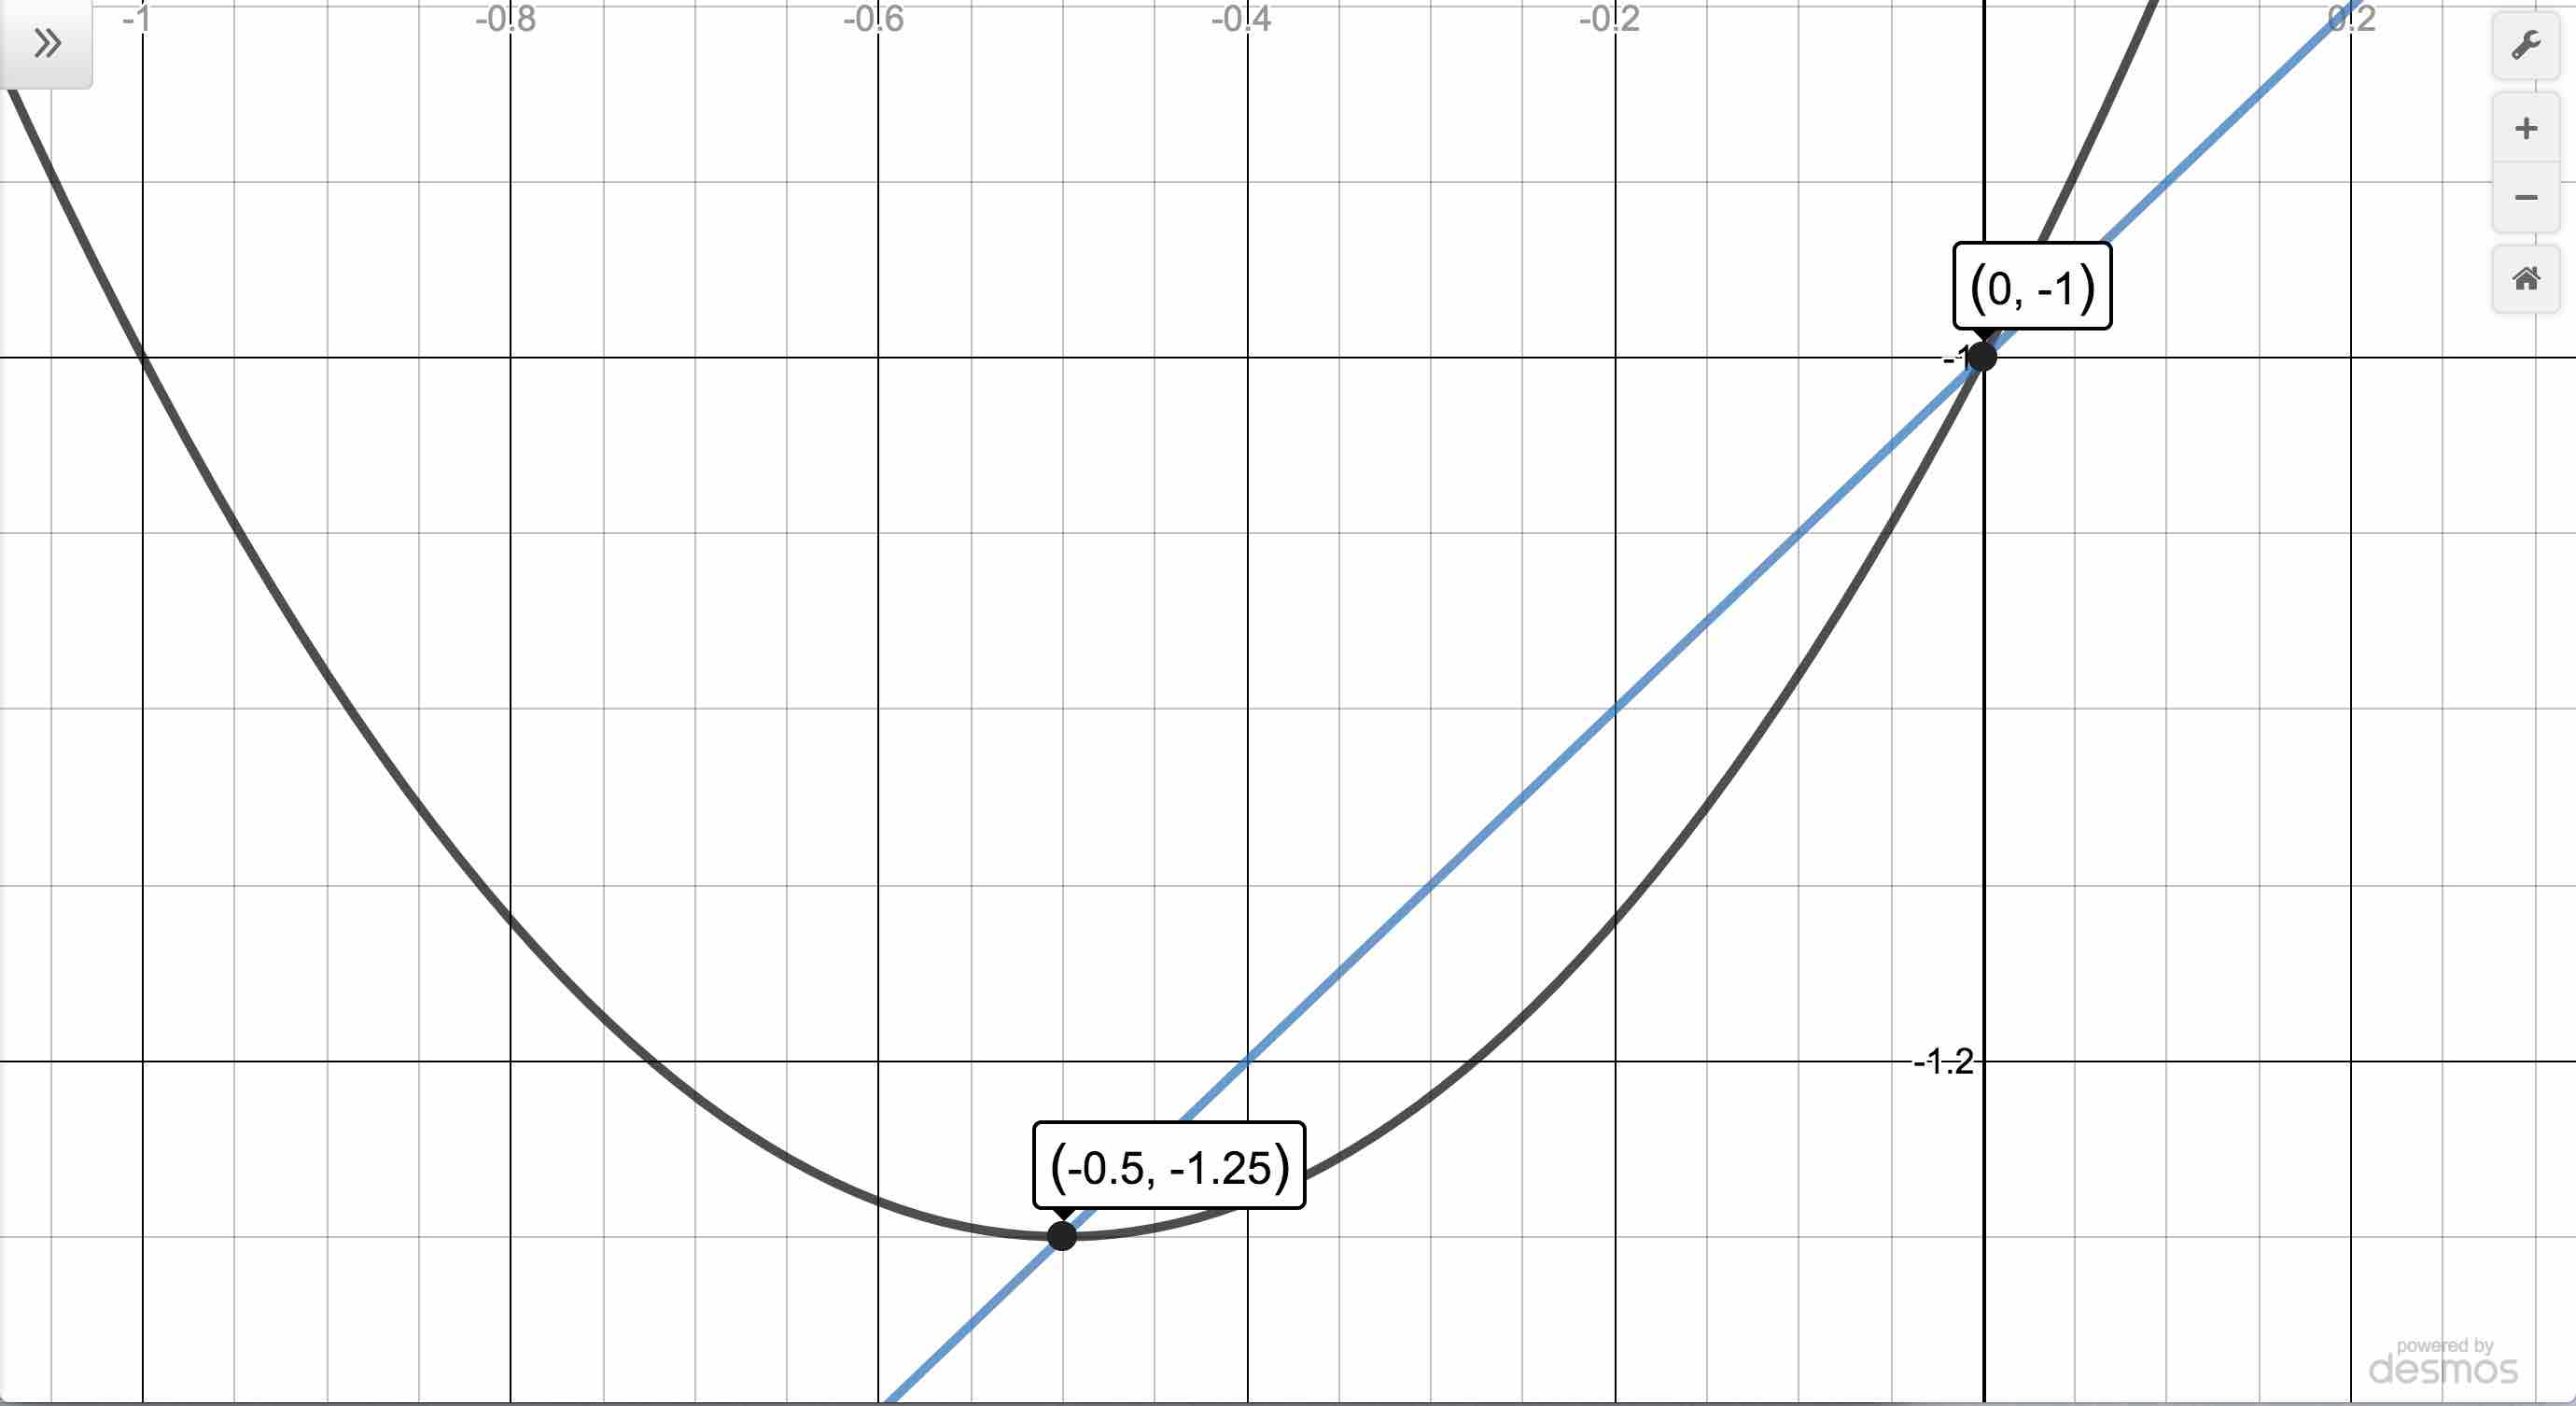
\includegraphics[width=2.75in]{./RationalIneqGraphics/RatIneqEx01.jpg} & 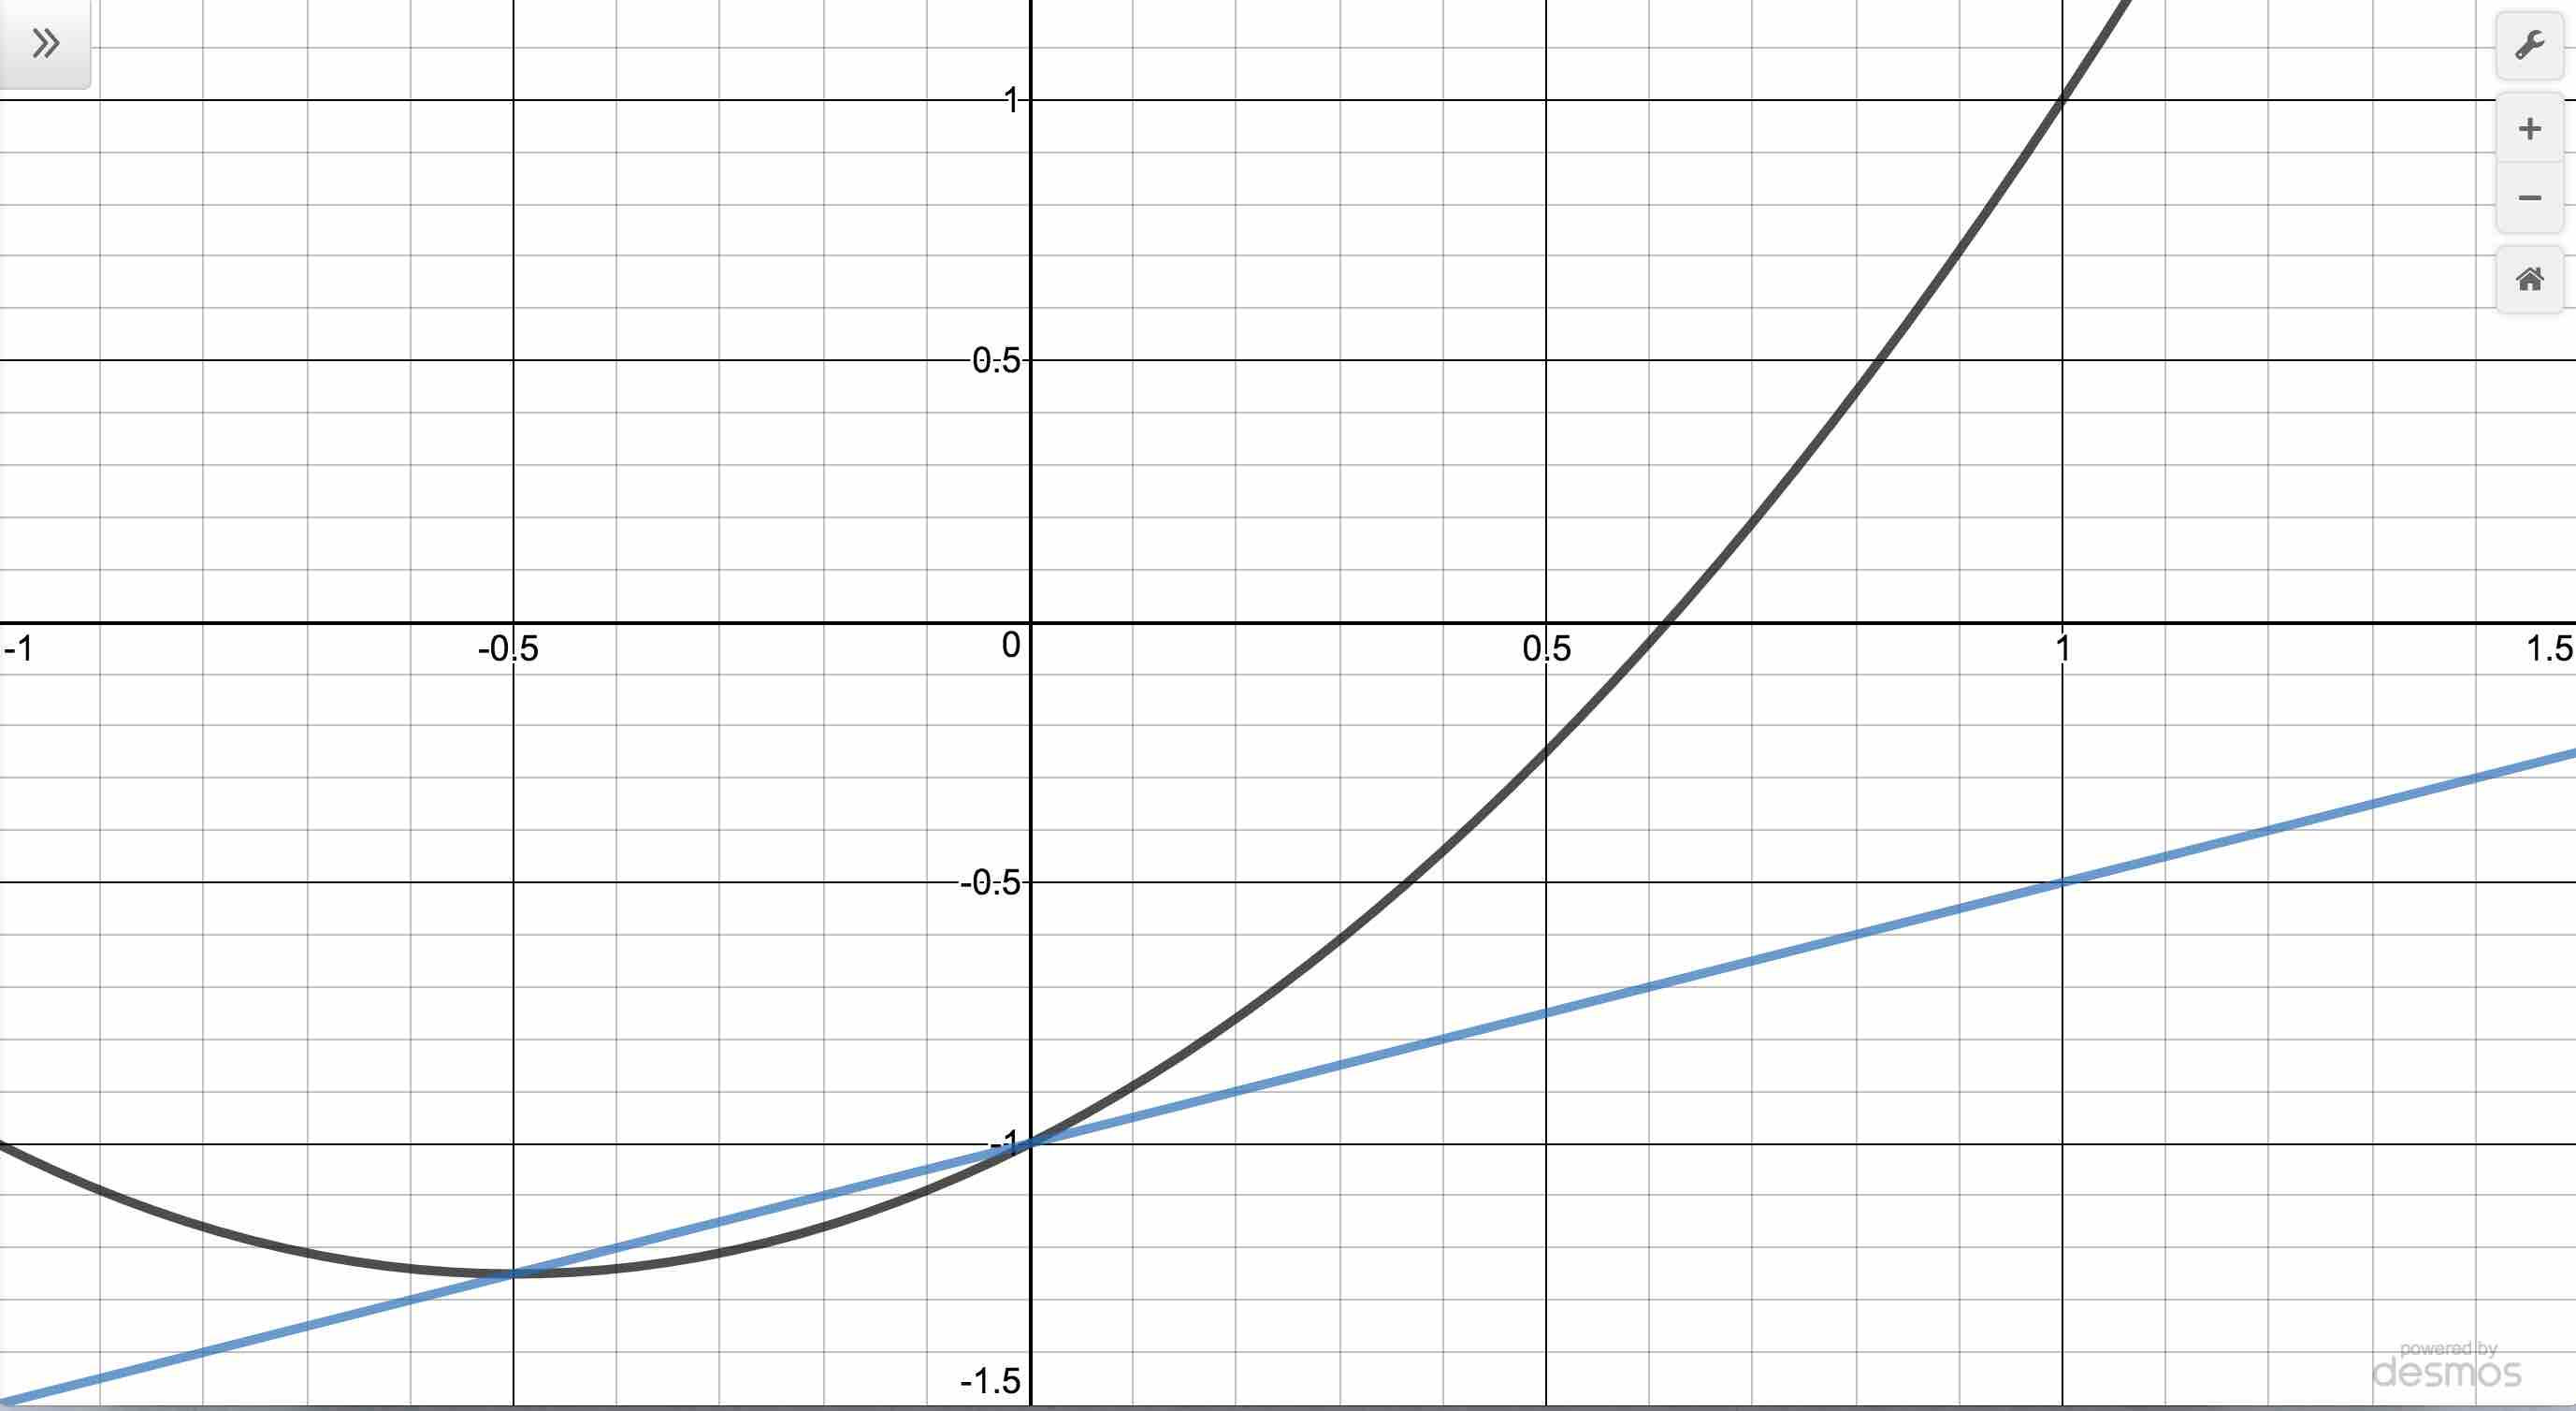
\includegraphics[width=2.75in]{./RationalIneqGraphics/RatIneqEx02.jpg}


\end{tabular}

\end{center} 

 \qed

\end{enumerate}
\end{ex}  

The important take-away from Example \ref{rationalinequalityex} is not to clear fractions when working with an inequality unless you know for certain the sign of the denominators. We offer another example.

\begin{ex} \label{morerationalineq} Solve:  $2t (3t-2)^{-1} \leq 3t^2 (3t-2)^{-2}$. Check your answer using a graphing utility.


{\bf Solution.} We begin by rewriting the terns with negative exponents as fractions and gathering all nonzero terms to one side of the inequality:

\[ \begin{array}{rclr}

2t (3t-2)^{-1} &  \leq & 3t^2 (3t-2)^{-2} & \\ [10pt]

\dfrac{2t}{3t-2} & \leq & \dfrac{3t^2}{(3t-2)^2} & \\ [10pt]


\dfrac{2t}{3t-2}  - \dfrac{3t^2}{(3t-2)^2}  & \leq & 0 &  \\ [10pt]

\dfrac{2t(3t-2)}{(3t-2)^2}  - \dfrac{3t^2}{(3t-2)^2}  & \leq & 0  & \text{get a common denominator} \\ [10pt]

\dfrac{2t(3t-2) - 3t^2}{(3t-2)^2}  & \leq & 0  &\\ [10pt]

\dfrac{3t^2-4t}{(3t-2)^2}  & \leq & 0  & \text{expand} \\ [10pt]

\end{array} \]

We define $r(t) = \frac{3t^2-4t}{(3t-2)^2}$ and set about constructing a sign diagram for $r$.  Solving  $(3t-2)^2 = 0$ gives $t = \frac{2}{3}$, our sole excluded value.  To find the zeros of $r$, we set $r(t) = \frac{3t^2-4t}{(3t-2)^2} = 0$ and solve $3t^2-4t = 0$.  Factoring gives $t(3t-4) = 0$ so our solutions are $t = 0$ and $t = \frac{4}{3}$. After choosing test values, we  get the sign diagram below on the left.   Since we are looking for where $r(t) \leq 0$, we are looking for where $r(t)$ is $(-)$ or $r(t) = 0$. Hence,  our final answer is $\left[0, \frac{2}{3} \right) \cup \left(\frac{2}{3}, \frac{4}{3} \right]$.  Below on the right,  we graph $f(t) = 2t(3t-1)^{-1}$ (the darker curve),   $g(t) = 3t^2(3t-2)^{-2}$, and  vertical asymptote $x = \frac{2}{3}$, the dashed line.  Sure enough, the graph of $f$ intersects the graph of $g$ when $t = 0$ and $t = \frac{4}{3}$.  Moreover, the graph of $f$ is below the graph of $g$ everywhere they are defined between these values, in accordance with our algebraic solution.

\begin{tabular}{m{2.5in}m{2.5in}}

\begin{mfpic}[10]{-6}{6}{-2}{2}
\arrow \reverse \arrow \polyline{(-6,0),(6,0)}
\xmarks{-3,0,3}
\tlpointsep{6pt}
\axislabels {x}{{$0 \hspace{7pt}$ } -3, {$\frac{2}{3}$} 0, {$\frac{4}{3}$} 3 }
\tlabel[cc](-4.5,1){$(+)$}
\tlabel[cc](-3,1){$0$}
\tlabel[cc](-1.5,1){$(-)$}
\tlabel[cc](0,1){\textinterrobang}
\tlabel[cc](1.5,1){$(-)$}
\tlabel[cc](3,1){$0$}
\tlabel[cc](4.5,1){$(+)$}
\end{mfpic} 

&

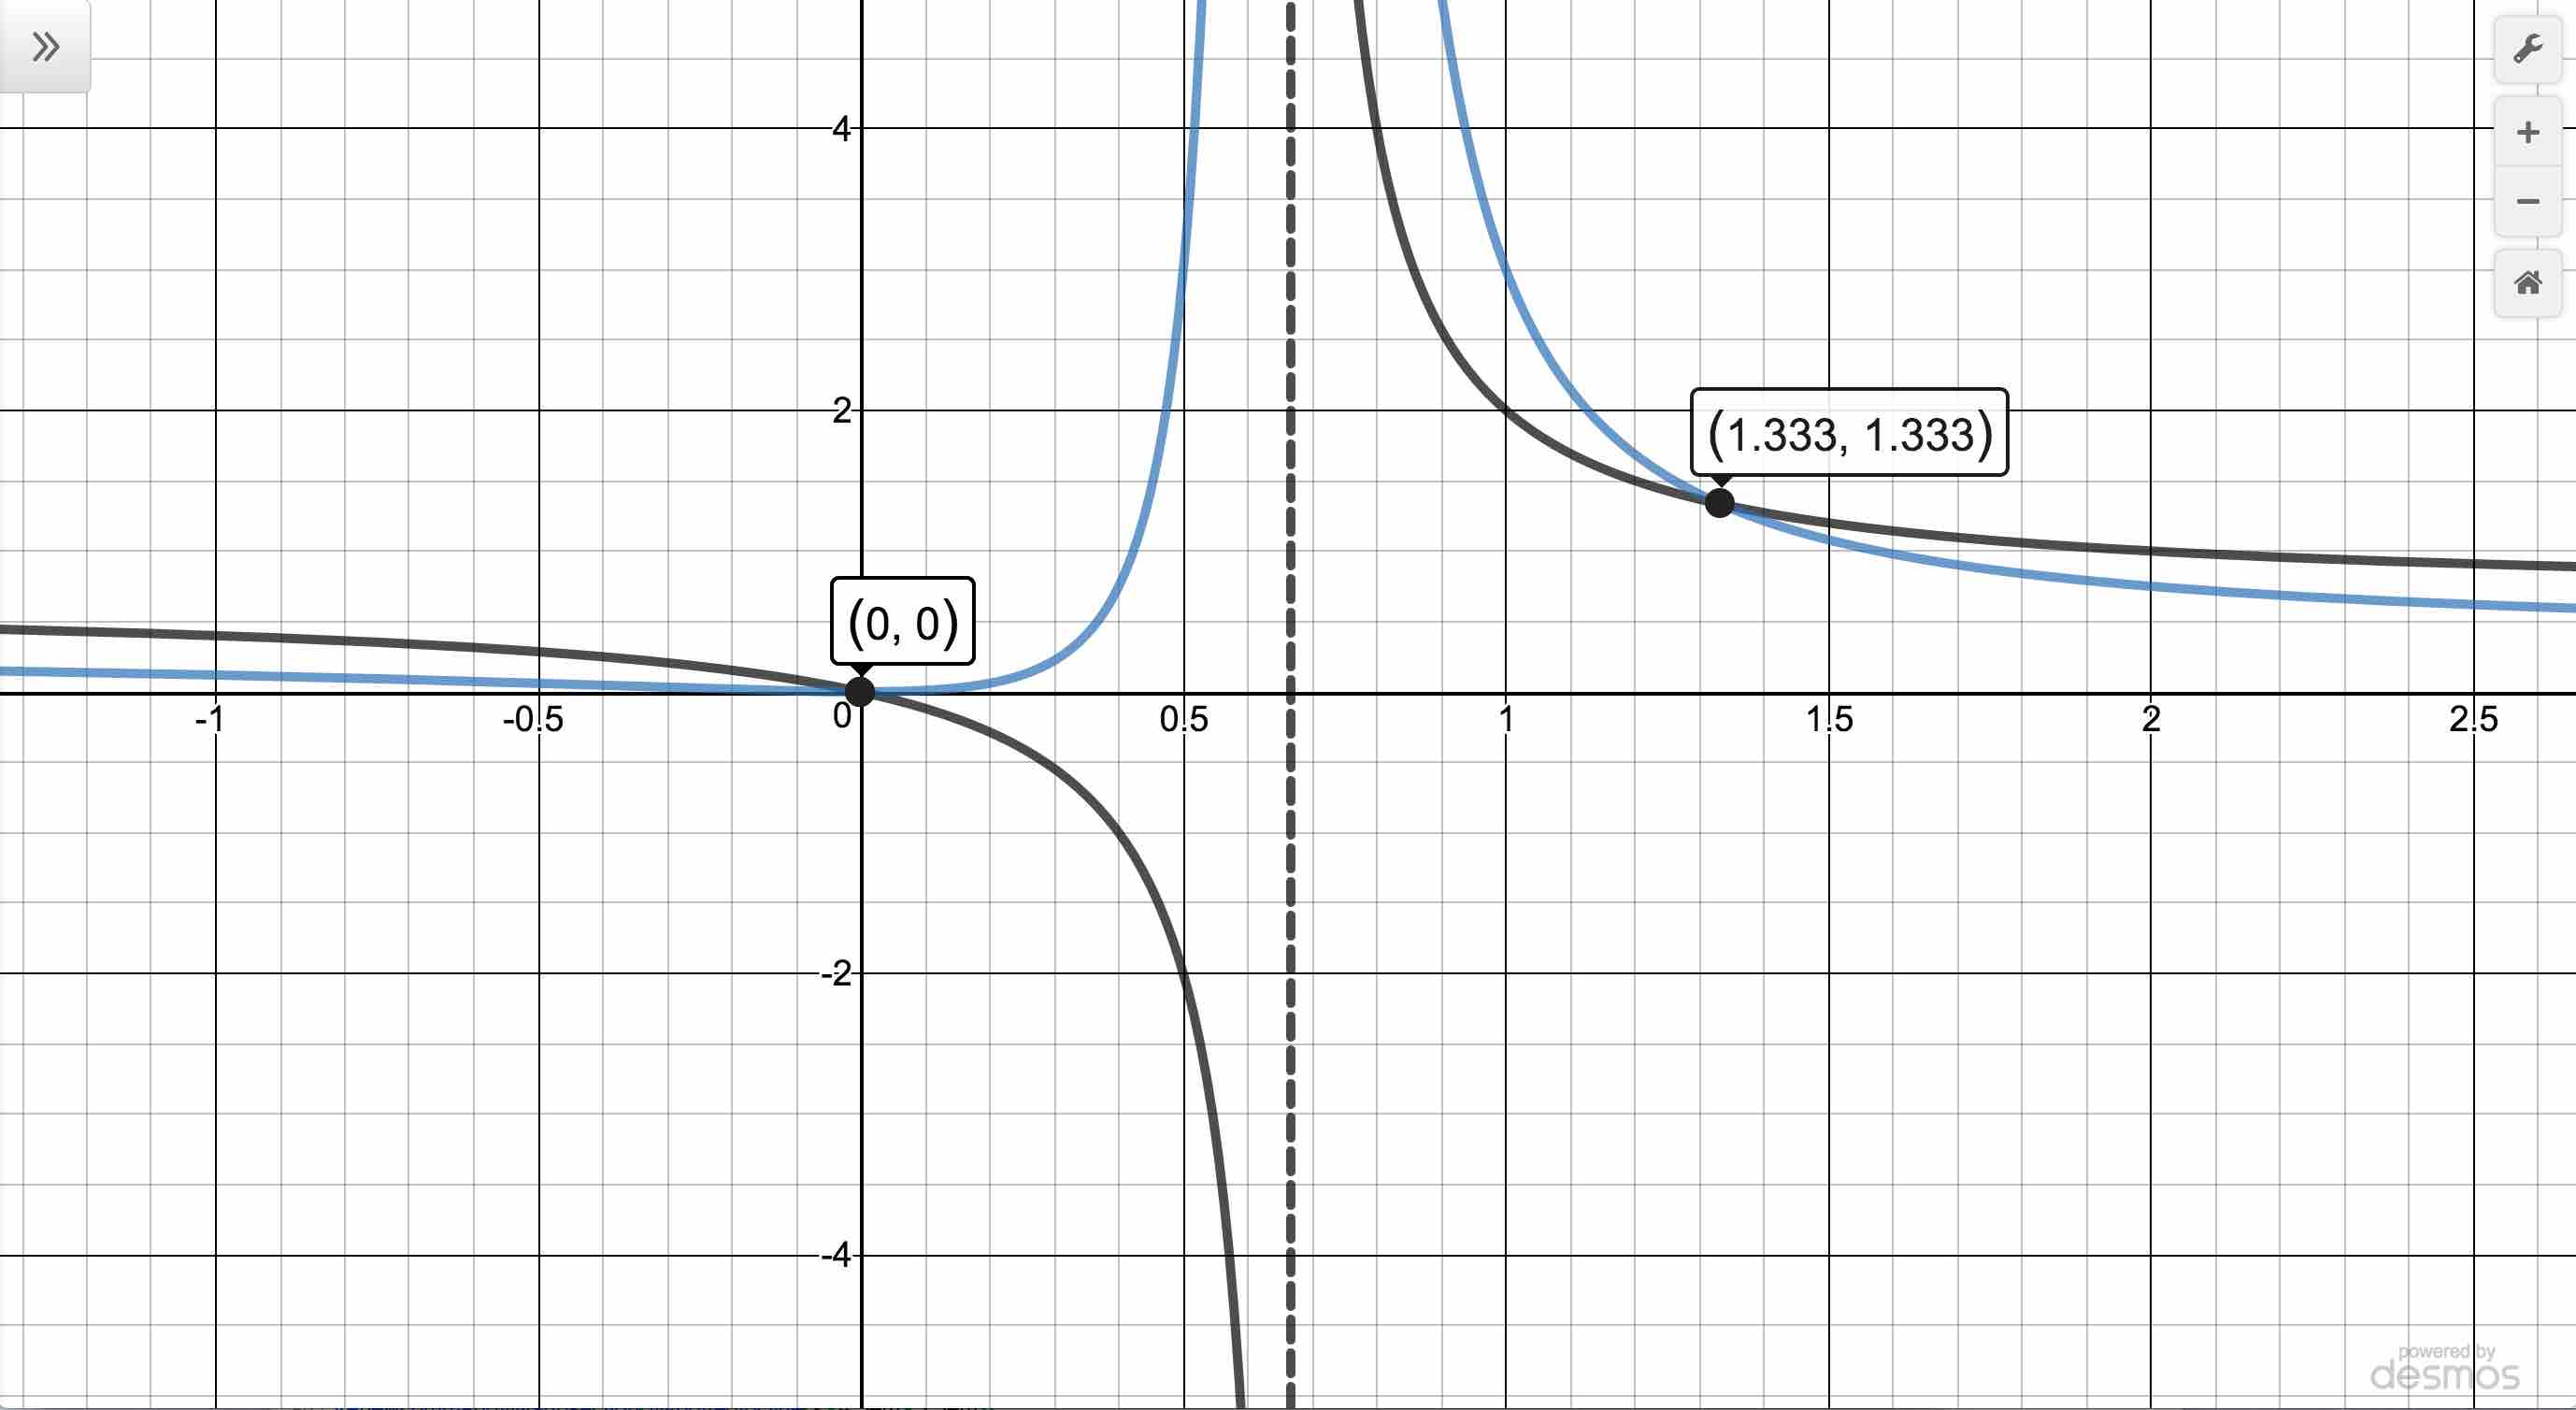
\includegraphics[width=2.75in]{./RationalIneqGraphics/RatIneqEx03.jpg} \\

\end{tabular}


\qed
\end{ex}

One thing to note about Example \ref{morerationalineq} is that the quantity $(3t-2)^2 \geq 0$ for all values of $t$.  Hence, as long as we remember $t = \frac{2}{3}$ is excluded from consideration, we could actually multiply both sides of the inequality in  Example \ref{morerationalineq} by $(3t-2)^2$ to obtain $2t(3t-2) \leq 3t^2$.  We could then solve this (slightly easier) inequality using the methods of Section \ref{QuadraticFunctions} as long as we remember to exclude $t = \frac{2}{3}$  from our solution. Once again, the more you \textit{understand}, the less you have to \textit{memorize}.  If you know the `\textit{why}' behind an algorithm instead of just the `\textit{how},' you will know when you can short-cut it.

Our next example is an application of average cost.  Recall from Definition \ref{averagecostprofit} if $C(x)$ represents the cost to make $x$ items then the average cost per item  is given by $\overline{C}(x) = \frac{C(x)}{x}$, for $x>0$. 

\begin{ex} \label{averagecostapp} Recall from Example \ref {PortaBoyCost} that the cost,  $C(x)$, in dollars, to produce $x$ PortaBoy game systems for a local retailer is $C(x) = 80x + 150$, $x \geq 0$.

\begin{enumerate}

\item  Find an expression for the average cost function, $\overline{C}(x)$. 

\item  \label{costlessthan} Solve $\overline{C}(x) < 100$ and interpret.

\item  Determine the behavior of $\overline{C}(x)$ as $x \rightarrow \infty$ and interpret.


\end{enumerate}

{\bf Solution.}

\begin{enumerate}

\item  From $\overline{C}(x) = \frac{C(x)}{x}$, we obtain $\overline{C}(x) = \frac{80x+150}{x}$.  The domain of $C$ is $x \geq 0$, but since $x=0$ causes problems for $\overline{C}(x)$, we get our domain to be $x>0$, or $(0, \infty)$.

\item  Solving $\overline{C}(x) < 100$ means we solve $\frac{80x+150}{x} < 100$.  We proceed as in the previous example.

\[ \begin{array}{rclr}

\dfrac{80x+150}{x} & < & 100 & \\ [10pt]

\dfrac{80x+150}{x} - 100 & < & 0 & \\ [10pt]

\dfrac{80x + 150 - 100x}{x} & < & 0 & \text{common denominator} \\ [10pt]

\dfrac{150 - 20x}{x} & < & 0 & \\

\end{array} \]

If we take the left hand side to be a rational function $r(x)$, we need to keep in mind that the applied domain of the problem is $x > 0$.  This means we consider only the positive half of the number line for our sign diagram.  On $(0, \infty)$, $r$ is defined everywhere so we need only look for zeros of $r$.  Setting $r(x)=0$ gives $150-20x =0$, so that $x = \frac{15}{2}= 7.5$.  The test intervals on our domain are $(0, 7.5)$ and $(7.5, \infty)$.  We find $r(x) < 0$ on $(7.5, \infty)$.  

\begin{center}

\begin{mfpic}[10]{0}{8}{-2}{2}
\arrow \polyline{(0,0), (8,0)}
\xmarks{0,4}
\tlabel[cc](0,-1){$0$}
\tlabel[cc](0,1){\textinterrobang}
\tlabel[cc](4,-1){$7.5$}
\tlabel[cc](2,1){$(+)$}
\tlabel[cc](4,1){$0$}
\tlabel[cc](6,1){$(-)$}
\end{mfpic}

\end{center}

In the context of the problem, $x$ represents the number of PortaBoy games systems produced and $\overline{C}(x)$ is the average cost to produce each system.  Solving $\overline{C}(x) < 100$ means we are trying to find how many systems we need to produce so that the average cost is less than $\$100$ per system.  Our solution, $(7.5, \infty)$ tells us that we need to produce more than $7.5$ systems to achieve this.  Since it doesn't make sense to produce half a system, our final answer is $[8, \infty)$.

\item  When we apply Theorem \ref{hathm} to $\overline{C}(x)$ we find that $y=80$ is a horizontal asymptote to the graph of $y=\overline{C}(x)$.  To more precisely determine the behavior of $\overline{C}(x)$ as $x \rightarrow \infty$, we first use long division\footnote{In this case, long division amounts to term-by-term division.} and rewrite $\overline{C}(x) = 80+\frac{150}{x}$.  As $x \rightarrow \infty$, $\frac{150}{x} \rightarrow 0^{+}$, which means $\overline{C}(x) \approx 80 + \text{very small $(+)$}$.  Thus the average cost per system is getting closer to $\$ 80$ per system.  If we set $\overline{C}(x) = 80$, we get $\frac{150}{x} = 0$, which is impossible, so we conclude that $\overline{C}(x) > 80$ for all $x > 0$.  This means that the average cost per system is always greater than $\$ 80$ per system, but the average cost is approaching this amount as more and more systems are produced.  Looking back at Example \ref{PortaBoyCost}, we realize $\$ 80$ is the variable cost per system $-$ the cost per system above and beyond the fixed initial cost of $\$150$.  Another way to interpret our answer is that `infinitely' many systems would need to be produced to effectively `zero out'  the fixed cost. \qed

\end{enumerate}

\end{ex}

Note that number \ref{costlessthan} in Example \ref{averagecostapp} is another opportunity to short-cut the standard algorithm and obtain the solution more quickly if we take stock of the situation.  Since the applied domain is $x>0$, we can multiply through the inequality $\frac{80x+150}{x}  <  100$ by $x$ without worrying about changing the sense of the inequality.  This reduces the problem to  $80x+150 < 100x$, a basic linear inequality whose solution is readily seen to be $x > 7.5$.   It is absolutely critical here that $x>0$. Indeed, any time you decide to multiply an inequality by a variable expression, it is necessary to justify why the inequality is preserved.  Our next example is another classic `box with no top' problem.  The reader is encouraged to compare and contrast this problem with  Example \ref{boxnotopex} in Section \ref{GraphsofPolynomials}.

\begin{ex}  \label{boxnotopfixedvolume} A box with a square base and no top is to be constructed so that it has a volume of $1000$ cubic centimeters.  Let $x$ denote the width of the box, in centimeters as seen below.

\begin{center}

\begin{mfpic}[15]{-2}{8}{-2}{4}
\polyline{(0,0),(0,1)}
\polyline{(4,0), (4,1)}
\polyline{(0,1),(2,3)}
\polyline{(4,1),(6,3)}
\polyline{(0,0),(4,0)}
\polyline{(0,1),(4,1)}
\polyline{(2,3),(6,3)}
\polyline{(4,0),(6,2)}
\polyline{(6,3),(6,2)}
\polyline{(2,3),(2,2)}
\polyline{(2,2),(5,2)}
\dotted \polyline{(5,2),(6,2)}
\polyline{(2,2),(1,1)}
\dotted \polyline{(1,1),(0,0)}
\arrow \reverse \arrow \polyline{(0,-0.5),(4,-0.5)}
\tlabel[cc](2,-1.5){\scriptsize width, $x$}
\arrow \reverse \arrow \polyline{(-0.5,0), (-0.5,1)}
\tlabel[cc](-1.5,0.5){\scriptsize height}
\arrow \reverse \arrow \polyline{(4.5, -0.25), (6.5,1.75)}
\tlabel[cc](6,0.25){\scriptsize depth}
\end{mfpic}


\end{center}


\begin{enumerate}

\item  Explain why the height of the box (in centimeters) is a function of the width $x$. Call this function $h$ and find an expression for $h(x)$, complete with an appropriate applied domain.

\item  Solve $h(x) \geq x$ and interpret.

\item  Find and interpret the behavior of $h(x)$ as $x \rightarrow 0^{+}$ and as $x \rightarrow \infty$.

\item  Express the surface area of the box as a function of $x$, $S(x)$ and state the applied domain.

\item  Use a graphing utility  to approximate (to two decimal places) the dimensions of the box which minimize the surface area.

\end{enumerate}

{ \bf Solution.}

\begin{enumerate}

\item  We are told that the volume of the box is $1000$ cubic centimeters and that $x$ represents the width, in centimeters.  Since $x$ represents a physical dimension of a box, we have that $x>0$.  From geometry, we know $\text{volume} = \text{width} \times \text{height} \times \text{depth}$.  Since the base of the box is a square, the width and the depth are both $x$ centimeters.  Hence,  $1000 = x^2 (\text{height})$. Solving for the height, we get $\text{height} = \frac{1000}{x^2}$.   In other words, for each width $x>0$, we are able to compute \textit{the}\footnote{that is, the one and only one} corresponding height using the formula $\frac{1000}{x^2}$.  Hence, the height is a function of $x$.    Using function notation, we write $h(x) = \frac{1000}{x^2}$.  As mentioned before, our only restriction is $x>0$ so the domain of $h$ is $(0, \infty)$.

\item  To solve $h(x) \geq x$, we proceed as before and collect all nonzero terms on one side of the inequality in order to use a sign diagram.

\[ \begin{array}{rclr}

h(x) & \geq & x & \\ [10pt]

\dfrac{1000}{x^2} & \geq & x & \\ [10pt]

\dfrac{1000}{x^2} - x & \geq & 0 \\ [10pt]

\dfrac{1000-x^3}{x^2} & \geq & 0 & \text{common denominator} \\[10pt]

\end{array} \]

We consider the left hand side of the inequality as our rational function $r(x)$.  We see immediately the only value excluded from the domain of $r$ is $0$, but since our applied domain is $x>0$, we restrict our attention to the interval  $(0, \infty)$.  The sole zero of $r$ comes when $1000-x^3 = 0$,  or when $x=10$.  Choosing test values in the intervals $(0,10)$ and $(10, \infty)$ gives the following:

\begin{center}

\begin{mfpic}[10]{0}{8}{-2}{2}

\arrow \polyline{(0,0), (8,0)}

\xmarks{0,4}

\tlabel[cc](0,-1){$0$}

\tlabel[cc](0,1){\textinterrobang}

\tlabel[cc](2,1){$(+)$}

\tlabel[cc](4,-1){$10$}

\tlabel[cc](4,1){$0$}

\tlabel[cc](6,1){$(-)$}

\end{mfpic}

\end{center}

We see $r(x) > 0$ on $(0,10)$, and since $r(x) = 0$ at $x=10$, our solution is $(0,10]$.  In the context of the problem, $h(x)$ represents the height of the box while $x$ represents the width (and depth) of the box.  Solving $h(x) \geq x$ is tantamount to finding the values of $x$ which result in a box where the height is at least as big as the width (and, in this case, depth.)  Our answer tells us the width of the box can be at most $10$ centimeters for this to happen.\footnote{As with the previous example, knowing $x>0$ means  $x^2>0$ so we can clear denominators right away and solve $x^3 \leq 1000$, or $x \leq 10$.  Coupled with our applied domain, $x>0$, we would arrive at the same solution, $(0, 10]$.}

\item As $x \rightarrow 0^{+}$, $h(x) = \frac{1000}{x^2} \rightarrow \infty$.  This means that the smaller the width $x$  (and, in this case, depth), the larger the height $h$ has to be in order to maintain a volume of $1000$ cubic centimeters. As $x \rightarrow \infty$, we find $h(x) \rightarrow 0^{+}$, which means that in order to maintain a volume of $1000$ cubic centimeters, the width and depth must get bigger as the height becomes smaller.

\item  Since the box has no top, the surface area can be found by adding the area of each of the sides to the area of the base.  The base is a square of dimensions $x$ by $x$, and each side has dimensions $x$ by $h(x)$.  We get the surface area, $S(x) = x^2+4xh(x)$.  Since $h(x) = \frac{1000}{x^2}$, we have  $S(x) = x^2+4x \left( \frac{1000}{x^2}\right)= x^2 + \frac{4000}{x}$.  The domain of $S$ is the same as $h$, namely $(0, \infty)$, for the same reasons as above.

\item   To graph $y = S(x)$, we create a table of values to help us define a good viewing window.  Doing so, we find a local minim when $x \approx 12.60$.  As far as we can tell,\footnote{without Calculus, that is...} this is the only local extremum, so it is the (absolute) minimum as well. This means that the width and depth of the box should each measure approximately $12.60$ centimeters.  To determine the height, we find $h(12.60) \approx 6.30$, so the height of the box should be approximately $6.30$ centimeters.\footnote{The $y$-coordinate here, $476.22$ means the minimum surface area possible is $476.22$ square centimeters.  Minimizing the surface area minimizes the material required to make the box, therein helping to reduce the cost of the box.}

\begin{center}


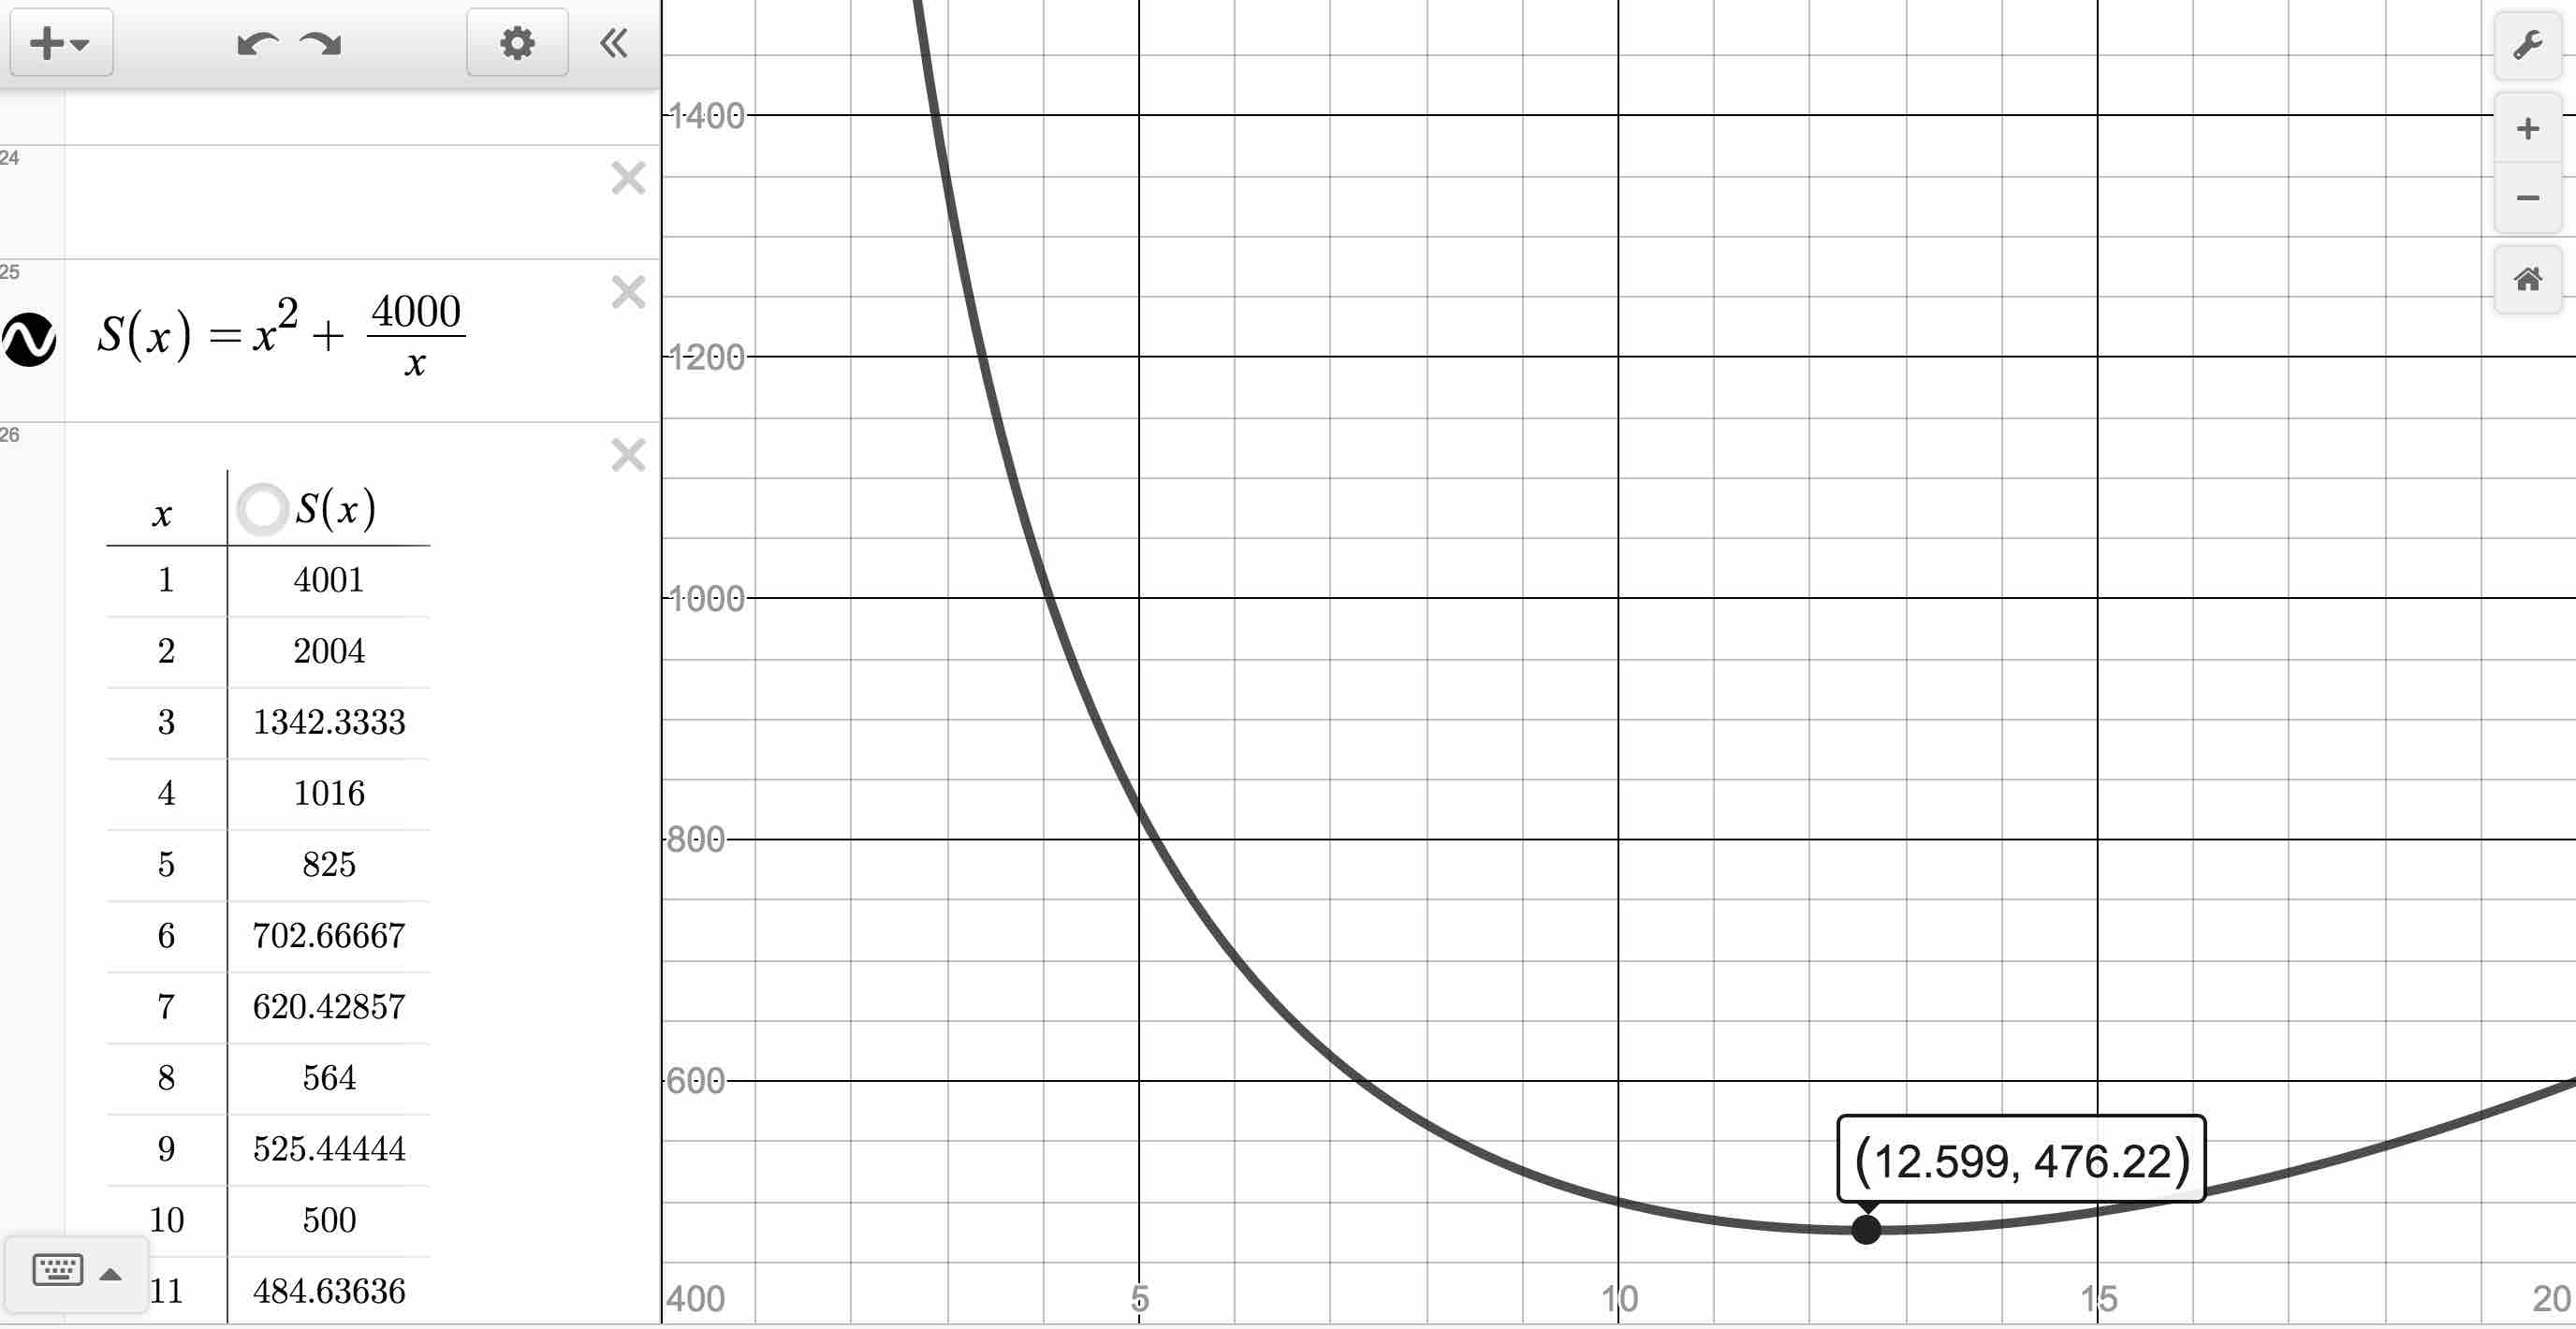
\includegraphics[width=4in]{./RationalIneqGraphics/RatIneqEx04.jpg} 


\end{center} 

\end{enumerate}
\qed

\end{ex}

Our last example uses regression to verify a very famous scientific law.

\begin{ex}  \label{BoyleslawRational} Boyle's Law states that when temperature is held constant, the pressure of a gas is inversely proportional to the volume of the gas.\footnote{For a review of what this means, see Section \ref{AppVariation}.}  According to this \href{http://web.lemoyne.edu/~giunta/classicalcs/boyleverify.html}{\underline{website}} the actual data relating the volume $V$ of a gas and its pressure $P$ used by Boyle and his assistant in 1662 to formulate this law is given below. (NOTE: both pressure and volume here are given in `arbitrary units.')

\[ \begin{array}{|c||c|c|c|c|c|c|c|c|c|c|c|c|c|}  \hline

V & 48 & 46 & 44 & 42 & 40 & 38 & 36 & 34 & 32 & 30 & 28 & 26 & 24  \\ \hline

P & 29.13 & 30.56 & 31.94 & 33.5 & 35.31 & 37 & 39.31 & 41.63 & 44.19 & 47.06 & 50.31 & 54.31 & 58.81  \\ \hline \end{array} \]


\[\begin{array}{|c||c||c|c|c|c|c|c|c|c|c|c|c|c|} \hline

V & 23 & 22 & 21 & 20 & 19 & 18 & 17 & 16 & 15 & 14 & 13 & 12  \\ \hline 

P & 61.31 & 64.06 & 67.06 & 70.69 & 74.13 & 77.88 & 82.75 & 87.88 & 93.06 & 100.44 & 107.81 & 117.56   \\ \hline \end{array} \]

\begin{enumerate}

\item Assuming  $P$ and $V$ are inversely proportional, estimate  the constant of proportionality, $k$.

\item Use a graphing utility to fit a curve of the form $P = \dfrac{k}{V}$ to these data.  

\end{enumerate}
 
{\bf Solution.}

\begin{enumerate}

\item Recall if $P$ and $V$ are inversely proportional, there is a real number $k$ so $PV = k$ for all values of $P$ and $V$.  Multiplying the corresponding $P$ and $V$ values from the data together result in numbers which are consistently approximately $1400$.  This gives us confidence in the claim $P$ and $V$ are inversely proportional and suggests $k \approx 1400$.

\item  We plot the pairs $(V, P)$ and run a regression, the results of which are below.  To our amazement, the graphing utility reports $k \approx 1406.9$ with  $R^2 \approx 1$.  This means the data are a very good fit to the model $P = \frac{k}{V}$, or $PV = k$, hence verifying Boyle's Law for this set of data.

\begin{center}

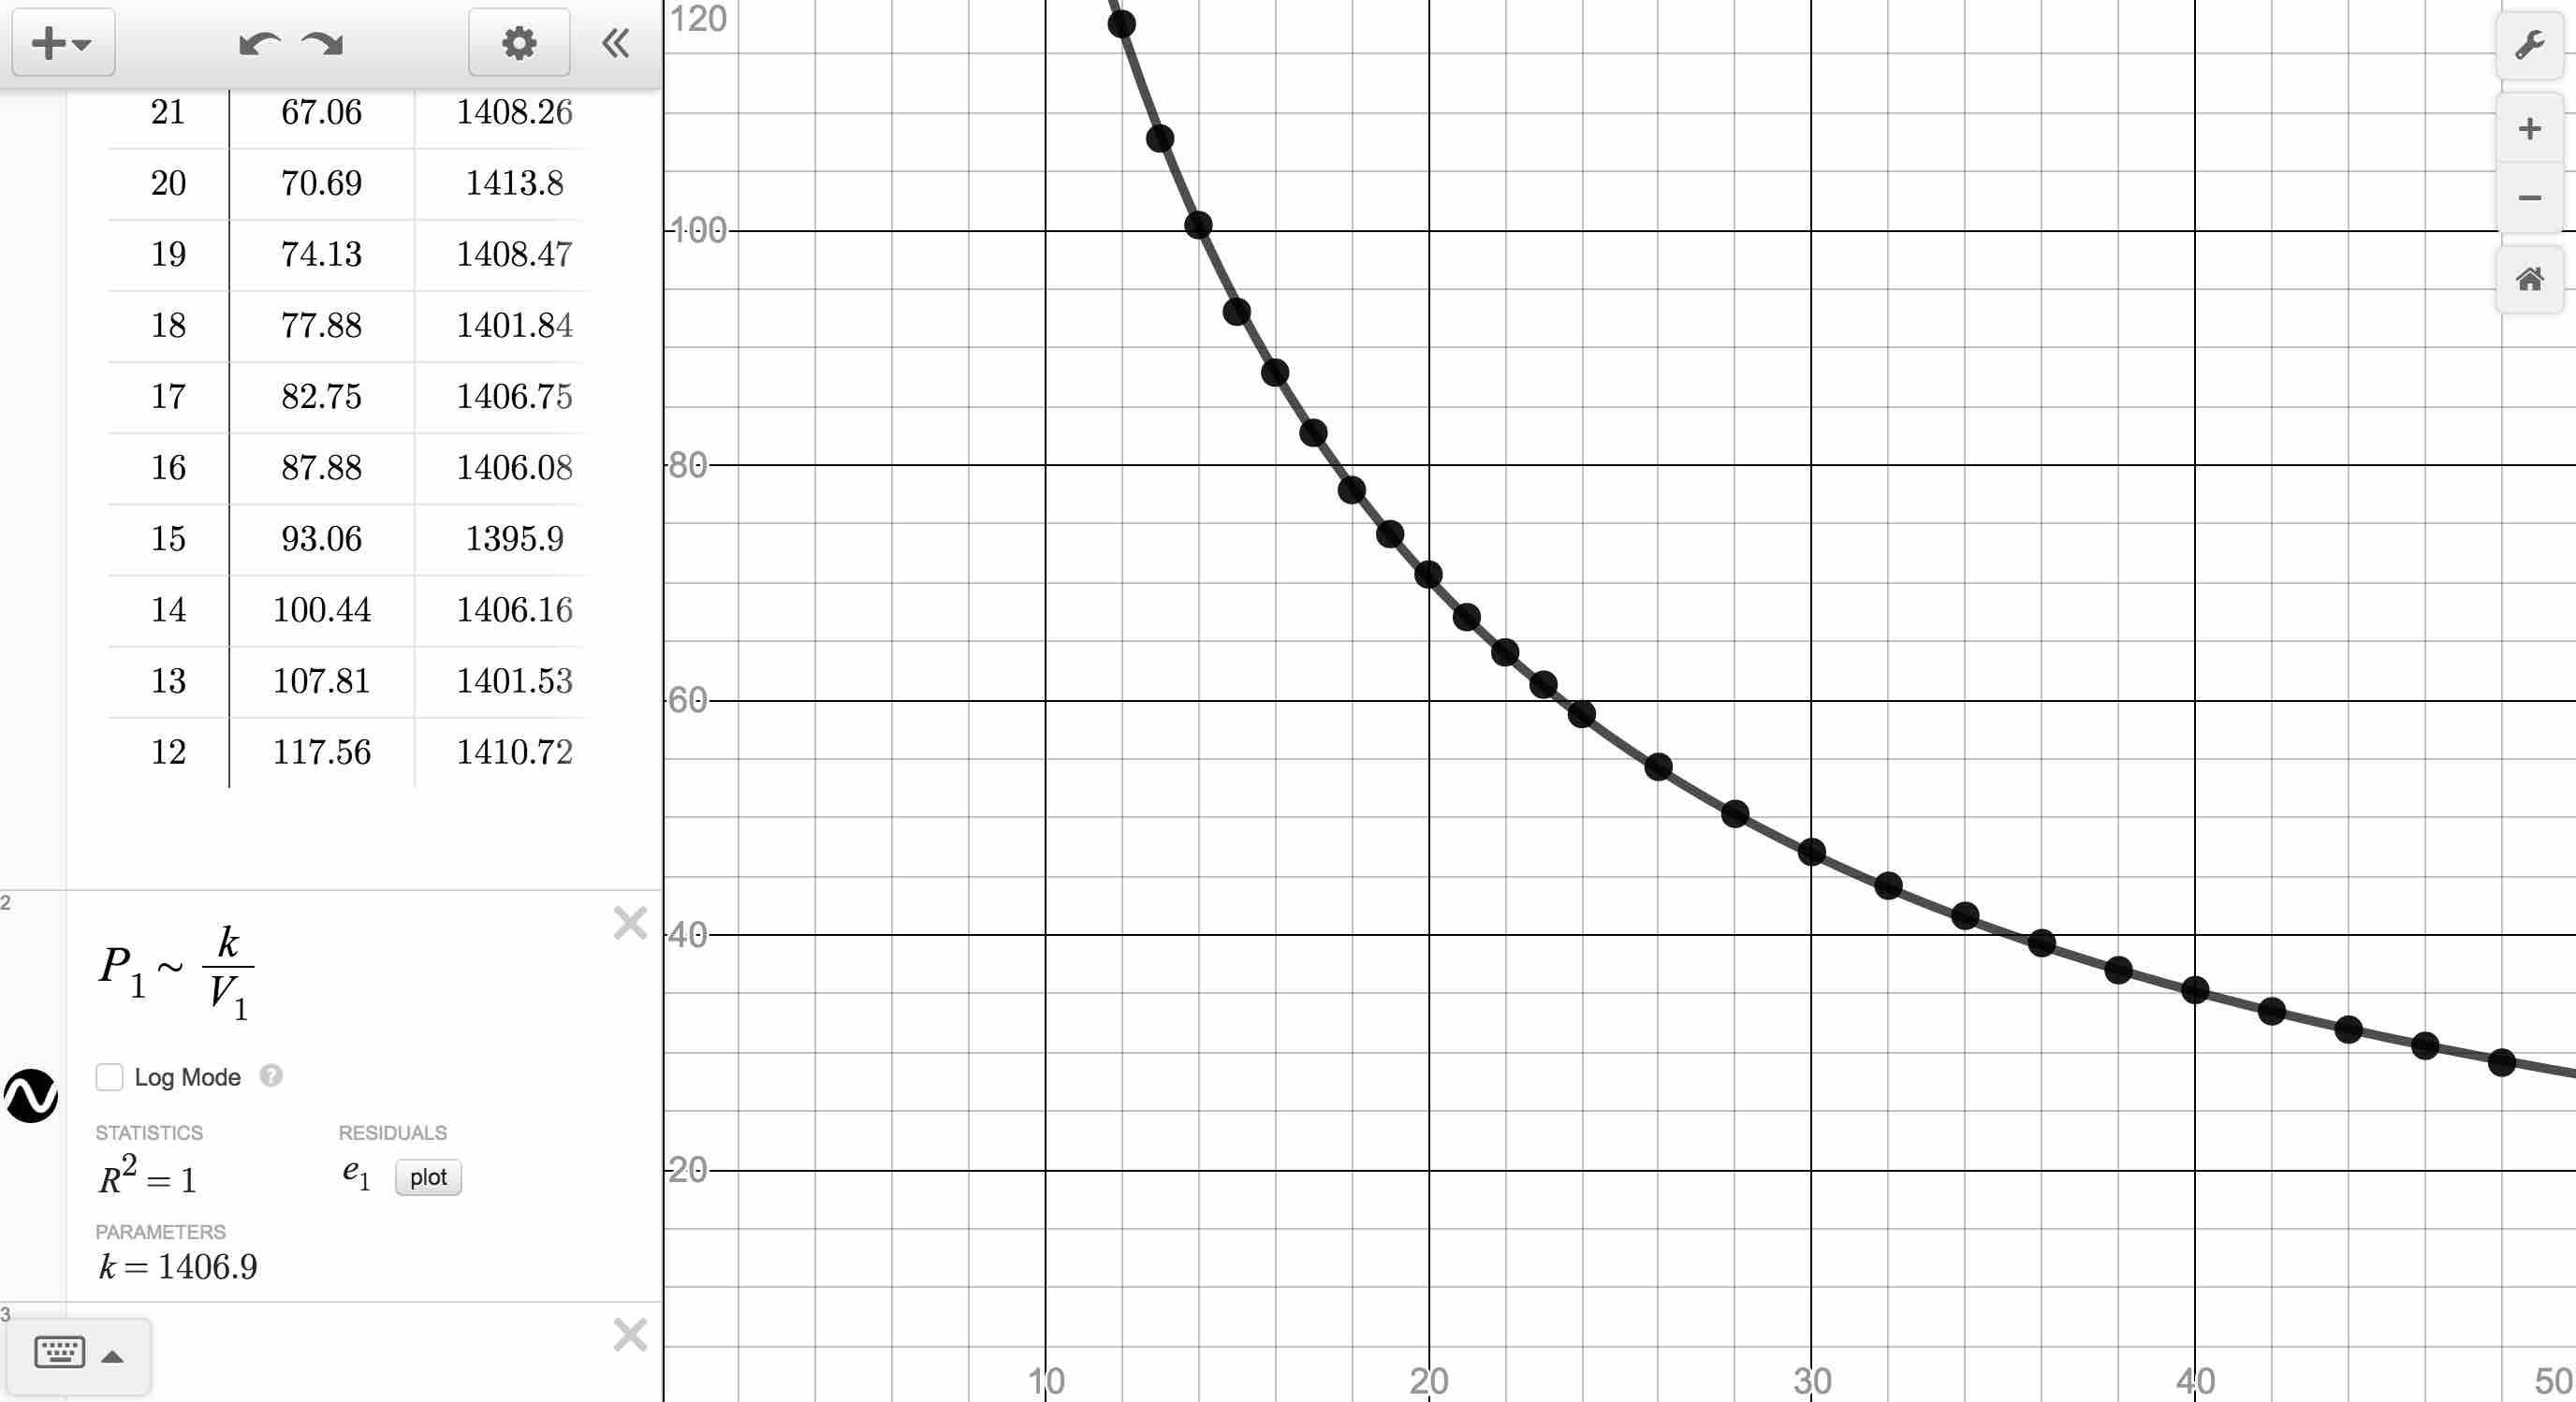
\includegraphics[width=6in]{./RationalIneqGraphics/BoylesLawEx.jpg} 

\end{center}


\end{enumerate}
\qed

\end{ex}

\newpage

\subsection{Exercises}

(Review of Solving Equations):\footnote{For more review, see Section \ref{AppRatExpEqus}.} In Exercises \ref{ratleqnexercisefirst} - \ref{ratleqnexerciselast},  solve the rational equation.  Be sure to check for extraneous solutions.

\begin{multicols}{2}
\begin{enumerate}

\item $\dfrac{x}{5x + 4} = 3$ \label{ratleqnexercisefirst}
\item $\dfrac{3x - 1}{x^{2} + 1} = 1$

\setcounter{HW}{\value{enumi}}
\end{enumerate}
\end{multicols}

\begin{multicols}{2}
\begin{enumerate}
\setcounter{enumi}{\value{HW}}

\item $\dfrac{1}{t + 3} + \dfrac{1}{t - 3} = \dfrac{t^{2} - 3}{t^{2} - 9}$
\item $\dfrac{2t + 17}{t + 1} = t + 5$

\setcounter{HW}{\value{enumi}}
\end{enumerate}
\end{multicols}

\begin{multicols}{2}
\begin{enumerate}
\setcounter{enumi}{\value{HW}}
\item $\dfrac{z^{2} - 2z + 1}{z^{3} + z^{2} - 2z} = 1$
\item $\dfrac{4z- z^3}{z^{2} - 9} = 4z$  \label{ratleqnexerciselast}

\setcounter{HW}{\value{enumi}}
\end{enumerate}
\end{multicols}

In Exercises \ref{ratlineqexercisefirst} - \ref{ratlineqexerciselast}, solve the rational inequality.  Express your answer using interval notation.

\begin{multicols}{3}
\begin{enumerate}
\setcounter{enumi}{\value{HW}}

\item $\dfrac{1}{x + 2} \geq 0$ \label{ratlineqexercisefirst}
\item $\dfrac{5}{x + 2} \geq 1$
\item $\dfrac{x}{x^{2} - 1} <  0$

\setcounter{HW}{\value{enumi}}
\end{enumerate}
\end{multicols}

\begin{multicols}{3}
\begin{enumerate}
\setcounter{enumi}{\value{HW}}


\item  $\dfrac{4t}{t^2+4} \geq 0$
\item  $\dfrac{2t+6}{t^2+t-6} < 1$
\item  $\dfrac{5}{t-3} + 9 < \dfrac{20}{t+3}$

\setcounter{HW}{\value{enumi}}
\end{enumerate}
\end{multicols}

\begin{multicols}{3}
\begin{enumerate}
\setcounter{enumi}{\value{HW}}


\item  $\dfrac{6z+6}{2+z-z^2} \leq z+3$
\item $\dfrac{6}{z-1} + 1 > \dfrac{1}{z+1}$
\item $\dfrac{3z - 1}{z^{2} + 1} \leq 1$

\setcounter{HW}{\value{enumi}}
\end{enumerate}
\end{multicols}

\begin{multicols}{3}
\begin{enumerate}
\setcounter{enumi}{\value{HW}}

\item $(2x+17)(x+1)^{-1} > x + 5$
\item $(4x-x^3)(x^{2} - 9)^{-1} \geq 4x$
\item $(x^{2} + 1)^{-1} < 0$ 

\setcounter{HW}{\value{enumi}}
\end{enumerate}
\end{multicols}

\begin{multicols}{2}
\begin{enumerate}
\setcounter{enumi}{\value{HW}}

\item $(2t-8)(t+1)^{-1} \leq (t^2-8t)(t+1)^{-2}$ % $[-4, -1) \cup (-1,2]$
\item $(t-3)(2t+7)(t^2+7t+6)^{-2} \geq (t^2+7t+6)^{-1}$ % $(-\infty, -6) \cup (-6, -3] \cup [9, \infty)$

\setcounter{HW}{\value{enumi}}
\end{enumerate}
\end{multicols}

\begin{multicols}{2}
\begin{enumerate}
\setcounter{enumi}{\value{HW}}

\item $60z^{-2}+23z^{-1} \geq 7(z-4)^{-1}$
\item $2z+6(z-1)^{-1} \geq 11 - 8(z+1)^{-1}$ \label{ratlineqexerciselast}

\setcounter{HW}{\value{enumi}}
\end{enumerate}
\end{multicols}

In Exercises \ref{solverationalineqfromgraphfirst} - \ref{solverationalineqfromgraphlast}, use the the graph of the given rational function to  solve the stated inequality.

\begin{multicols}{2}
\begin{enumerate}
\setcounter{enumi}{\value{HW}}

\item \label{solverationalineqfromgraphfirst} Solve $f(x) \geq 0$.


\begin{mfpic}[10]{-7}{7}{-6}{8}
%\point[4pt]{(-3,2), (-1,4), (1,-2), (3,0)}
\point[4pt]{(3,0)}
\dashed \polyline{(-7,1), (7,1)}
\tlabel[cc](7,-0.5){\scriptsize $x$}
\tlabel[cc](0.5,8){\scriptsize $y$}
\tlabel[cc](3.5,-1){\scriptsize $(3,0)$}
\axes
\xmarks{-6 step 1 until 6}
\ymarks{-5 step 1 until 7}
\tiny
\tlpointsep{4pt}
\axislabels {x}{{$-6 \hspace{7pt}$} -6, {$-5 \hspace{7pt}$} -5, {$-4 \hspace{7pt}$} -4, {$-3\hspace{7pt}$} -3, {$-2\hspace{7pt}$} -2, {$-1\hspace{7pt}$} -1,  {$1$} 1, {$5$} 5, {$6$} 6}
\axislabels {y}{{$-5$} -5, {$-4$} -4, {$-3$} -3, {$-2$} -2, {$-1$} -1, {$1$} 1, {$2$} 2, {$3$} 3, {$4$} 4}
\normalsize
\penwd{1.25pt}
\arrow \reverse \arrow \function{-7,-0.45,0.1}{1 - (3/x)}
\arrow \reverse \arrow  \function{0.45,7,0.1}{1 - (3/x)}
\tcaption{\scriptsize  $y=f(x)$, asymptotes: $x = 0$, $y=1$.}
\end{mfpic}

\vfill

\columnbreak

\item  Solve $f(x) < 1$.


\begin{mfpic}[10]{-7}{7}{-6}{8}
%\point[4pt]{(-3,2), (-1,4), (1,-2), (3,0)}
\point[4pt]{(3,0)}
\dashed \polyline{(-7,1), (7,1)}
\tlabel[cc](7,-0.5){\scriptsize $x$}
\tlabel[cc](0.5,8){\scriptsize $y$}
\tlabel[cc](3.5,-1){\scriptsize $(3,0)$}
\axes
\xmarks{-6 step 1 until 6}
\ymarks{-5 step 1 until 7}
\tiny
\tlpointsep{4pt}
\axislabels {x}{{$-6 \hspace{7pt}$} -6, {$-5 \hspace{7pt}$} -5, {$-4 \hspace{7pt}$} -4, {$-3\hspace{7pt}$} -3, {$-2\hspace{7pt}$} -2, {$-1\hspace{7pt}$} -1,  {$1$} 1, {$5$} 5, {$6$} 6}
\axislabels {y}{{$-5$} -5, {$-4$} -4, {$-3$} -3, {$-2$} -2, {$-1$} -1, {$1$} 1, {$2$} 2, {$3$} 3, {$4$} 4}
\normalsize
\penwd{1.25pt}
\arrow \reverse \arrow \function{-7,-0.45,0.1}{1 - (3/x)}
\arrow \reverse \arrow  \function{0.45,7,0.1}{1 - (3/x)}
\tcaption{\scriptsize  $y=f(x)$, asymptotes: $x = 0$, $y=1$.}
\end{mfpic}


\setcounter{HW}{\value{enumi}}
\end{enumerate}
\end{multicols}


\begin{multicols}{2}
\begin{enumerate}
\setcounter{enumi}{\value{HW}}

\item   Solve $g(t) \geq  -1 $. 

\begin{mfpic}[18]{-2}{6}{-4}{4}
\axes
\xmarks{-1 step 1 until 5}
\ymarks{-3,-2,1,2,3}
\point[4pt]{(1,-1), (3,1)}
\dashed \polyline{(2,-4), (2,4)}
\tlabel[cc](6,-0.5){\scriptsize $t$}
\tlabel[cc](0.5,4){\scriptsize $y$}
\tlabel[cc](3.75,1.25){\scriptsize $(3,1)$}
\gclear \tlabelrect(0, -1.25){\scriptsize $(1,-1)$}

\tiny
\tlpointsep{4pt}
\axislabels {x}{{$-1\hspace{7pt}$} -1,  {$1$} 1, {$2$} 2, {$3$} 3, {$4$} 4}
\axislabels {y}{{$-3$} -3, {$-2$} -2, {$1$} 1,  {$2$} 2, {$3$} 3}
\normalsize
\penwd{1.25pt}
\arrow \reverse \arrow \function{-2,1.75,0.1}{1/(x-2)}
\arrow \reverse \arrow  \function{2.25,6,0.1}{1/(x-2)}
\tcaption{\scriptsize  $y=g(t)$, asymptotes: $t = 2$, $y=0$.}
\end{mfpic}

\vfill

\columnbreak

\item  Solve $-1 \leq g(t)  < 1$. 

\begin{mfpic}[18]{-2}{6}{-4}{4}
\axes
\xmarks{-1 step 1 until 5}
\ymarks{-3,-2,1,2,3}
\point[4pt]{(1,-1), (3,1)}
\dashed \polyline{(2,-4), (2,4)}
\tlabel[cc](6,-0.5){\scriptsize $t$}
\tlabel[cc](0.5,4){\scriptsize $y$}
\tlabel[cc](3.75,1.25){\scriptsize $(3,1)$}
\gclear \tlabelrect(0, -1.25){\scriptsize $(1,-1)$}
\tiny
\tlpointsep{4pt}
\axislabels {x}{{$-1\hspace{7pt}$} -1,  {$1$} 1, {$2$} 2, {$3$} 3, {$4$} 4}
\axislabels {y}{{$-3$} -3, {$-2$} -2, {$1$} 1,  {$2$} 2, {$3$} 3}
\normalsize
\penwd{1.25pt}
\arrow \reverse \arrow \function{-2,1.75,0.1}{1/(x-2)}
\arrow \reverse \arrow  \function{2.25,6,0.1}{1/(x-2)}
\tcaption{\scriptsize  $y=g(t)$, asymptotes: $t = 2$, $y=0$.}
\end{mfpic}

\setcounter{HW}{\value{enumi}}
\end{enumerate}
\end{multicols}


\begin{multicols}{2}
\begin{enumerate}
\setcounter{enumi}{\value{HW}}

\item  Solve $r(z) \leq 1$ 

\begin{mfpic}[15][20]{-5}{5}{-1}{6}
\tlabel[cc](5,-0.5){\scriptsize $z$}
\tlabel[cc](0.5,6){\scriptsize $y$}
\tlabel[cc](-2.5,1){\scriptsize $(-1,1)$}
\tlabel[cc](3,1){\scriptsize hole at $(1,1)$}
\axes
\xmarks{-4 step 1 until 4}
\ymarks{1 step 1 until 5}
\tiny
\tlpointsep{4pt}
\axislabels {x}{{$-4 \hspace{7pt}$} -4, {$-3\hspace{7pt}$} -3, {$-2\hspace{7pt}$} -2, {$-1\hspace{7pt}$} -1,  {$1$} 1, {$2$} 2, {$3$} 3, {$4$} 4}
\axislabels {y}{{$1$} 1, {$2$} 2, {$3$} 3, {$4$} 4, {$5$} 5}
\normalsize
\penwd{1.25pt}
\arrow \reverse \arrow \function{-5,-0.42,0.1}{1/(x**2)}
\arrow \reverse \arrow  \function{0.42,5,0.1}{1/(x**2)}
\point[4pt]{(-1,1)}
\pointfillfalse
\point[4pt]{(1,1)}
\tcaption{\scriptsize $y = r(z)$, asymptotes:  $z=0$, $y=0$.}
\end{mfpic}


\vfill

\columnbreak


\item \label{solverationalineqfromgraphlast} Solve $r(z) > 0$.


\begin{mfpic}[15][20]{-5}{5}{-1}{6}
\tlabel[cc](5,-0.5){\scriptsize $z$}
\tlabel[cc](0.5,6){\scriptsize $y$}
\tlabel[cc](-2.5,1){\scriptsize $(-1,1)$}
\tlabel[cc](3,1){\scriptsize hole at $(1,1)$}
\axes
\xmarks{-4 step 1 until 4}
\ymarks{1 step 1 until 5}
\tiny
\tlpointsep{4pt}
\axislabels {x}{{$-4 \hspace{7pt}$} -4, {$-3\hspace{7pt}$} -3, {$-2\hspace{7pt}$} -2, {$-1\hspace{7pt}$} -1,  {$1$} 1, {$2$} 2, {$3$} 3, {$4$} 4}
\axislabels {y}{{$1$} 1, {$2$} 2, {$3$} 3, {$4$} 4, {$5$} 5}
\normalsize
\penwd{1.25pt}
\arrow \reverse \arrow \function{-5,-0.42,0.1}{1/(x**2)}
\arrow \reverse \arrow  \function{0.42,5,0.1}{1/(x**2)}
\point[4pt]{(-1,1)}
\pointfillfalse
\point[4pt]{(1,1)}
\tcaption{\scriptsize $y = r(z)$, asymptotes:  $z=0$, $y=0$.}
\end{mfpic}


\setcounter{HW}{\value{enumi}}
\end{enumerate}
\end{multicols}

\begin{enumerate}
\setcounter{enumi}{\value{HW}}


\item  In Exercise \ref{newportaboycost} in Section \ref{GraphsofPolynomials},  the function $C(x) = .03x^{3} - 4.5x^{2} + 225x + 250$, for $x \geq 0$ was used to model the cost (in dollars) to produce $x$ PortaBoy game systems. Using this cost function, find the number of PortaBoys which should be produced to minimize the average cost $\overline{C}$.  Round your answer to the nearest number of systems. 

\item  Suppose we are in the same situation as Example \ref{boxnotopfixedvolume}.  If the volume of the box is to be $500$ cubic centimeters, use a graphing utility to find the dimensions of the box which minimize the surface area.  What is the minimum surface area?  Round your answers to two decimal places.

\item  The box for the new Sasquatch-themed cereal, `Crypt-Os', is to have a volume of $140$ cubic inches.  For aesthetic reasons, the height of the box needs to be $1.62$ times the width of the base of the box.\footnote{1.62 is a crude approximation of the so-called `Golden Ratio' $\phi = \frac{1 + \sqrt{5}}{2}$.}  Find the dimensions of the box which will minimize the surface area of the box.  What is the minimum surface area?  Round your answers to two decimal places.   

\item \label{fixedareaminperimetergarden} Sally is Skippy's neighbor from Exercise \ref{fixedperimetermaxareagarden} in Section \ref{QuadraticFunctions}.   Sally also wants to plant a vegetable garden along the side of her home.  She doesn't have any fencing, but wants to keep the size of the garden to 100 square feet.  What are the dimensions of the garden which will minimize the amount of fencing she needs to buy?  What is the minimum amount of fencing she needs to buy? Round your answers to the nearest foot. (Note:  Since one side of the garden will border the house, Sally doesn't need fencing along that side.)



\item Another Classic Problem: A can is made in the shape of a right circular cylinder and is to hold one pint. (For dry goods, one pint is equal to $33.6$ cubic inches.)\footnote{According to \href{http://dictionary.reference.com/browse/pint}{\underline{www.dictionary.com}}, there are different values given for this conversion. We use $33.6 \text{in}^{3}$ for this problem.}  

\begin{enumerate}

\item Find an expression for the volume $V$ of the can in terms of the height $h$ and the base radius $r$.
\item Find an expression for the surface area $S$ of the can in terms of the height $h$ and the base radius $r$.  (Hint: The top and bottom of the can are circles of radius $r$ and the side of the can is really just a rectangle that has been bent into a cylinder.)
\item Using the fact that $V = 33.6$, write $S$ as a function of $r$ and state its applied domain.
\item Use your graphing calculator to find the dimensions of the can which has minimal surface area.

\end{enumerate}

\item  A right cylindrical drum is to hold 7.35 cubic feet of liquid.  Find the dimensions (radius of the base and height) of the drum which would minimize the surface area.  What is the minimum surface area?  Round your answers to two decimal places.


\item In Exercise \ref{squatchpop} in Section \ref{IntroRational}, the population of Sasquatch in Portage County is modeled by  \[P(t) = \frac{150t}{t + 15}, \quad t \geq 0,\] where $t = 0$ corresponds to the year 1803.  According to this model, when were there fewer than 100 Sasquatch in Portage County?

\setcounter{HW}{\value{enumi}}
\end{enumerate}



\newpage

\subsection{Answers}

\begin{multicols}{3} 
\begin{enumerate}

\item $x = -\frac{6}{7}$
\item $x = 1, \; x = 2$
\item $t = -1$

\setcounter{HW}{\value{enumi}}
\end{enumerate}
\end{multicols}

\begin{multicols}{3}
\begin{enumerate}
\setcounter{enumi}{\value{HW}}

\item $t = -6, \; x = 2$
\item No solution
\item $z = 0, \; z = \pm 2\sqrt{2}$

\setcounter{HW}{\value{enumi}}
\end{enumerate}
\end{multicols}

\begin{multicols}{2}
\begin{enumerate}
\setcounter{enumi}{\value{HW}}

\item $(-2, \infty)$
\item $(-2, 3]$

\setcounter{HW}{\value{enumi}}
\end{enumerate}
\end{multicols}

\begin{multicols}{2}
\begin{enumerate}
\setcounter{enumi}{\value{HW}}


\item $(-\infty, -1) \cup (0, 1)$
\item $[0, \infty)$

\setcounter{HW}{\value{enumi}}
\end{enumerate}
\end{multicols}

\begin{multicols}{2}
\begin{enumerate}
\setcounter{enumi}{\value{HW}}

\item $(-\infty, -3) \cup (-3,2) \cup (4, \infty)$
\item $\left(-3, -\frac{1}{3} \right) \cup (2,3)$

\setcounter{HW}{\value{enumi}}
\end{enumerate}
\end{multicols}

\begin{multicols}{2}
\begin{enumerate}
\setcounter{enumi}{\value{HW}}

\item $(-1,0] \cup (2, \infty)$
\item $(-\infty, -3) \cup (-2, -1) \cup (1, \infty)$

\setcounter{HW}{\value{enumi}}
\end{enumerate}
\end{multicols}

\begin{multicols}{2}
\begin{enumerate}
\setcounter{enumi}{\value{HW}}

\item $(-\infty, 1] \cup [2, \infty)$
\item $(-\infty, -6) \cup (-1, 2)$

\setcounter{HW}{\value{enumi}}
\end{enumerate}
\end{multicols}

\begin{multicols}{2}
\begin{enumerate}
\setcounter{enumi}{\value{HW}}

\item $(-\infty, -3) \cup \left[-2\sqrt{2}, 0\right] \cup \left[2\sqrt{2}, 3\right)$
\item No solution

\setcounter{HW}{\value{enumi}}
\end{enumerate}
\end{multicols}

\begin{multicols}{2}
\begin{enumerate}
\setcounter{enumi}{\value{HW}}

\item  $[-4, -1) \cup (-1,2]$
\item   $(-\infty, -6) \cup (-6, -3] \cup [9, \infty)$

\setcounter{HW}{\value{enumi}}
\end{enumerate}
\end{multicols}

\begin{multicols}{2}
\begin{enumerate}
\setcounter{enumi}{\value{HW}}

\item $[-3,0) \cup (0,4) \cup [5, \infty)$
\item  $\left(-1,-\frac{1}{2}\right] \cup (1, \infty)$

\setcounter{HW}{\value{enumi}}
\end{enumerate}
\end{multicols}

\begin{multicols}{2}
\begin{enumerate}
\setcounter{enumi}{\value{HW}}

\item $f(x) \geq 0$ on $(-\infty, 0) \cup [3, \infty)$.

\item $f(x) < 1$ on $(0, \infty)$.

\setcounter{HW}{\value{enumi}}
\end{enumerate}
\end{multicols}

\begin{multicols}{2}
\begin{enumerate}
\setcounter{enumi}{\value{HW}}

\item  $g(t) \geq -1$ on $(-\infty, 1] \cup (2, \infty)$.
\item  $-1 \leq g(t) < 1$ on $(-\infty, 1] \cup (3, \infty)$.

\setcounter{HW}{\value{enumi}}
\end{enumerate}
\end{multicols}

\begin{multicols}{2}
\begin{enumerate}
\setcounter{enumi}{\value{HW}}

\item  $r(z) \leq 1$ on $(-\infty, -1] \cup (1, \infty)$.

\item  $r(z) > 0$ on $(-\infty, 0) \cup (0,1) \cup (1, \infty)$.


\setcounter{HW}{\value{enumi}}
\end{enumerate}
\end{multicols}


\begin{enumerate}
\setcounter{enumi}{\value{HW}}

\item  The absolute minimum of $y=\overline{C}(x)$ occurs at $\approx (75.73, 59.57)$.  Since $x$ represents the number of game systems, we check $\overline{C}(75) \approx 59.58$ and $\overline{C}(76) \approx 59.57$.  Hence, to minimize the average cost, $76$ systems should be produced at an average cost of $\$59.57$ per system.

\item The width (and depth) should be $10.00$ centimeters, the height should be $5.00$ centimeters.  The minimum surface area is $300.00$ square centimeters.

\item The width of the base of the box should be approximately $4.12$ inches, the height of the box should be approximately $ 6.67$ inches, and the depth of the base of the box should be approximately $5.09$ inches. The minimum surface area is approximately $164.91$ square inches.

\newpage

\item The dimensions are  approximately  $7$ feet by $14$ feet.  Hence, the minimum amount of fencing required is approximately  $28$ feet.

\item 

\begin{multicols}{2}
\begin{enumerate}

\item $V = \pi r^{2}h$
\item $S = 2 \pi r^{2} + 2\pi r h$

\setcounter{HWindent}{\value{enumii}}
\end{enumerate}
\end{multicols}



\begin{multicols}{2}
\begin{enumerate}
\setcounter{enumii}{\value{HWindent}}

\item $S(r) = 2\pi r^{2} + \frac{67.2}{r}, \;$  Domain $r > 0$
\item $r \approx 1.749\,$in. and $h \approx 3.498\,$in. 

\end{enumerate}
\end{multicols}

\item  The radius of the drum should be approximately $1.05$ feet and the height of the drum should be approximately  $2.12$ feet.  The minimum surface area of the drum is approximately $20.93$ cubic feet.

\item $P(t) < 100$ on $(-15, 30)$, and the portion of this which lies in the applied domain is $[0,30)$.  Since $t=0$ corresponds to the year 1803, from 1803 through the end of 1832, there were fewer than 100 Sasquatch in Portage County.

\setcounter{HW}{\value{enumi}}
\end{enumerate}



\closegraphsfile

\newpage
\end{comment}


\end{document}